\documentclass[english,letterpaper]{article}%{scrartcl}
%\setkomafont{disposition}{\normalfont}  %KOMA use serif font for sectioning
\usepackage[T1]{fontenc}
\usepackage[latin9]{inputenc}
\usepackage{geometry}
\geometry{verbose,tmargin=2cm,bmargin=2.5cm,lmargin=1cm,rmargin=1cm}
\setlength{\parskip}{\smallskipamount}
\setlength{\parindent}{0pt}
\usepackage{color}
\usepackage{babel}
\usepackage{mathtools}
\usepackage{amsmath}
\usepackage{amsthm}
%\usepackage[amsthm]{ntheorem}
\usepackage{amssymb}
\usepackage{wasysym}
\usepackage{cancel}
\usepackage{imakeidx}
\usepackage{wrapfig}
\usepackage[stable]{footmisc}

\usepackage{stmaryrd}
\expandafter\def\csname opt@stmaryrd.sty\endcsname{only,shortleftarrow,shortrightarrow} %fake options for stmaryd so that loading extpfeil later doesn't cause a clash
\usepackage{extpfeil} % lets define multiple long arrows
\newextarrow{\toto}{{20}{20}{20}{20}}{\bigRelbar\bigRelbar{\bigtwoarrowsleft\rightarrow\rightarrow}}

   

\makeindex
\usepackage[footnotesize]{caption}
\captionsetup{width=0.6\textwidth}
\DeclareCaptionLabelFormat{bf-parens}{\textbf{Fig. #2}}
\captionsetup{labelformat=bf-parens}

\usepackage{comment}
\includecomment{comment}
%\excludecomment{comment}

%%%%%% FONTS
%\usepackage[onlytext,lf]{MinionPro}      % enable all this to get custom fonts
%\usepackage[amsbb,subscriptcorrection,mtpcal,mtphrb]{mtpro2}
%OR
%\usepackage{pscyr}
%\usepackage[libertine]{newtxmath}
%OR
\usepackage{newtxtext}
\usepackage[varvw]{newtxmath}

\usepackage{tikz-cd}
%\usepackage{marginnote}

\usepackage[activate={true},step=1,tracking=true,kerning=true,spacing=false,factor=1100,stretch=20,shrink=20]{microtype}%text appearance improvements
\UseMicrotypeSet[protrusion]{basictext}
%\microtypecontext{spacing=nonfrench}
%\DisableLigatures[N]{encoding=*, family =*}

\usepackage{titlesec} %change title spacing for sections
\titlespacing*{\section}
{0pt}{0.7\baselineskip}{0.3\baselineskip}
\titlespacing*{\subsection}
{0pt}{0.7\baselineskip}{0.3\baselineskip}


%%%%%%%
\usepackage[unicode=true,pdfusetitle,
 bookmarks=true,bookmarksnumbered=false,bookmarksopen=false,
 breaklinks=false,pdfborder={0 0 1},backref=false,colorlinks=true]
 {hyperref}
\usepackage{tocbibind}

\usepackage{enumitem}
\setlist[enumerate]{leftmargin=2em}
\setlist[itemize]{leftmargin=2em}



\makeatletter

%%%%%%%%%%%%%%%%%%%%%%%%%%%%%% Defining environments
\usepackage{silence}
\usepackage{mdframed}                        %  for frames around theorem environments
\WarningFilter{mdframed}{You got a bad break}  %block mdframed warnings about page breaks

\usepackage{xcolor} % For using `gray!20` for example
%--------------------------------
% Redefinition of `\newmdtheoremenv` for accepting a starred version
\DeclareDocumentCommand\newmdtheoremenv{s O{} m o m o }{%
\IfBooleanTF{#1}{%
   \newtheorem*{#3}{#5}%
 }{%
 \ifboolexpr{ test {\IfNoValueTF {#4}} and test {\IfNoValueTF {#6}} }%
    {\newtheorem{#3}{#5}}{%
     \IfValueTF{#4}{\newtheorem{#3}[#4]{#5}}{}%
     \IfValueTF{#6}{\newtheorem{#3}{#5}[#6]}{}%
    }
  }%
  \BeforeBeginEnvironment{#3}{%
     \begin{mdframed}[#2]}%
  \AfterEndEnvironment{#3}{%
     \end{mdframed}}%
}
%--------------------------------
\mdfdefinestyle{myshadedthm}{backgroundcolor=gray!20,linewidth=0pt,innerleftmargin=1ex,innerrightmargin=0.5ex,%
%--------------------------------
% If you use `amsthm` can adjust `innertopmargin` to avoid extra space in top.
innertopmargin=-0.5ex% % Comment or remove this line if you use `ntheorem`.
%--------------------------------
}
\mdfdefinestyle{linedthm}{linewidth=1pt,topline=false,bottomline=false,rightline=false,innertopmargin=-1ex,innerbottommargin=-0.3ex,innerleftmargin=1ex,innerrightmargin=0ex}
\mdfdefinestyle{indentthm}{hidealllines=true,innertopmargin=-1ex,innerbottommargin=-0.3ex,innerleftmargin=1ex,innerrightmargin=0ex}

\numberwithin{equation}{section}
\numberwithin{figure}{section}
\numberwithin{table}{section}
\theoremstyle{definition}
%\newtheorem{defn}{\protect\definitionname}[section]
\newmdtheoremenv[style=linedthm]{defn}{Definition}[section]
\theoremstyle{definition}
%\newtheorem{example}{\protect\examplename}[section]
\newmdtheoremenv[style=indentthm]{example}{\protect\examplename}[section]
\theoremstyle{definition}
%\newtheorem{xca}{\protect\exercisename}[section]
\newmdtheoremenv[style=indentthm]{xca}{\protect\exercisename}[section]
\theoremstyle{plain}
%\newtheorem{prop}{\protect\propositionname}[section]
\newmdtheoremenv[style=myshadedthm]{prop}{\protect\propositionname}[section]
\theoremstyle{plain}
%\newtheorem{thm}[prop]{\protect\theoremname}%thm with counter inherited from prop
\newmdtheoremenv[style=myshadedthm]{thm}[prop]{\protect\theoremname}
\theoremstyle{plain}
%\newtheorem{lem}[prop]{Lemma}%lem with counter inherited from prop
\newmdtheoremenv[style=myshadedthm]{lem}[prop]{Lemma}
\theoremstyle{plain}
%\newtheorem{cor}[prop]{Corollary}%cor with counter inherited from prop
\newmdtheoremenv[style=myshadedthm]{cor}[prop]{Corollary}
\theoremstyle{remark}
%\newtheorem*{rem*}{\protect\remarkname}
\newmdtheoremenv*[style=linedthm]{rem*}{\protect\remarkname}
\theoremstyle{remark}
%\newtheorem{rem}{\protect\remarkname}[section]
\newmdtheoremenv[style=linedthm]{rem}{\protect\remarkname}[section]
%%%%%%%%%%%%%%%%%%%%%%%%%%%%%% User specified LaTeX commands.

\renewenvironment{align*}{\align}{\endalign}
\renewenvironment{alignat*}{\alignat}{\endalignat}
\renewenvironment{multline*}{\multline}{\endmultline}
\renewenvironment{gather*}{\gather}{\endgather}
\renewenvironment{equation*}{\equation}{\endequation}


\usepackage{color}
\def\white{\color{white}}
\def\black{\color{black}}
\def\red{\color{red}}
\def\green{\color{green}}
\def\blue{\color{blue}}
\def\cyan{\color{cyan}}
\def\magenta{\color{magenta}}
\def\yellow{\color{yellow}}



\newcommand{\bbR}{\mathbb{R}}
\newcommand{\bbN}{\mathbb{N}}
\newcommand{\bbC}{\mathbb{C}}
\newcommand{\bbZ}{\mathbb{Z}}
\newcommand{\bbH}{\mathbb{H}}
\newcommand{\bbQ}{\mathbb{Q}}
\newcommand{\calC}{\mathcal{C}}
\newcommand{\calD}{\mathcal{D}}
\newcommand{\calJ}{\mathcal{J}}
\newcommand{\calE}{\mathcal{E}}
\newcommand{\calU}{\mathcal{U}}
\newcommand{\calV}{\mathcal{V}}

\newcommand{\dd}{{\mathrm{d}}}
\newcommand{\bm}[1]{\boldsymbol{\mathrm{#1}}}
\renewcommand{\geq}{\geqslant}
\renewcommand{\leq}{\leqslant}
\renewcommand{\i}{\mathrm{i}}
\renewcommand{\Re}{\operatorname{Re}}
\renewcommand{\Im}{\operatorname{Im}}
\DeclareMathOperator{\sign}{sign}
\DeclareMathOperator{\mor}{Mor}
\DeclareMathOperator{\id}{id}
\DeclareMathOperator{\ob}{Ob}
\DeclareMathOperator{\Mat}{Mat}
\DeclareMathOperator{\Aut}{Aut}
\DeclareMathOperator{\End}{End}
\DeclareMathOperator{\Int}{int}
\DeclareMathOperator{\im}{im}
\DeclareMathOperator{\rank}{rank}
\DeclareMathOperator{\pr}{pr}
\DeclareMathOperator{\supp}{supp}
\DeclareMathOperator{\Hom}{Hom}
\DeclareMathOperator{\Diff}{Diff}
\DeclareMathOperator{\Hol}{Hol}
\DeclareMathOperator{\GL}{GL}
\DeclareMathOperator{\Tr}{Tr}
\DeclareMathOperator{\tr}{tr}
\DeclareMathOperator{\proj}{pr}
\DeclareMathOperator{\codim}{codim}
\DeclareMathOperator{\Alt}{Alt}
\DeclareMathOperator{\Sym}{Sym}
\DeclareMathOperator{\grad}{grad}
\DeclareMathOperator{\coker}{coker}
\DeclareMathOperator{\coim}{coim}
\DeclareMathOperator{\Ext}{Ext}
\DeclareMathOperator{\Tor}{Tor}
\let\div\relax
\DeclareMathOperator{\div}{div}
\DeclareMathOperator*{\res}{res}
\newcommand{\colimit}{\varinjlim}
\newcommand{\limit}{\varprojlim}
\newcommand{\Lie}{\mathcal{L}}
\newcommand{\fX}{\mathfrak{X}}
\newcommand{\sub}{\vartriangleleft}
\newcommand{\sube}{\trianglelefteqslant}
\newcommand{\bigslant}[2]{{\raisebox{.2em}{$#1$}\left/\raisebox{-.2em}{$#2$}\right.}}

\usepackage{xparse}
\DeclareDocumentCommand{\restr}{m m o}  
{%
  \IfNoValueTF{#3}
  {
  \left.\kern-\nulldelimiterspace % automatically resize the bar with \right
  #1 % the function
  \vphantom{\big|} % pretend it's a little taller at normal size
  \right|_{#2}
  }{
  \left.\kern-\nulldelimiterspace % automatically resize the bar with \right
  #1 % the function
  \vphantom{\big|} % pretend it's a little taller at normal size
  \right|_{#2}^{#3} }
}

\makeatletter  %define \xoverline, automatically sized overline
\newsavebox\myboxA
\newsavebox\myboxB
\newlength\mylenA
\newcommand*\xoverline[2][0.75]{%
    \sbox{\myboxA}{$\m@th#2$}%
    \setbox\myboxB\null% Phantom box
    \ht\myboxB=\ht\myboxA%
    \dp\myboxB=\dp\myboxA%
    \wd\myboxB=#1\wd\myboxA% Scale phantom
    \sbox\myboxB{$\m@th\overline{\copy\myboxB}$}%  Overlined phantom
    \setlength\mylenA{\the\wd\myboxA}%   calc width diff
    \addtolength\mylenA{-\the\wd\myboxB}%
    \ifdim\wd\myboxB<\wd\myboxA%
       \rlap{\hskip 0.5\mylenA\usebox\myboxB}{\usebox\myboxA}%
    \else
        \hskip -0.5\mylenA\rlap{\usebox\myboxA}{\hskip 0.5\mylenA\usebox\myboxB}%
    \fi}
\makeatother

\usepackage{graphicx}
\newcommand{\PRLsep}{   %decorative line used to separate sections
           \noindent\makebox[\linewidth]{
                \resizebox{0.5\linewidth}{1pt}{$\blacklozenge$}}}

\usepackage{graphicx,scalerel}
\newcommand\wh[1]{\hstretch{1.42}{\hat{\hstretch{.7}{#1\mkern2mu}}}\mkern-2mu} %requires \usepackage{graphicx,scalerel}
\newcommand\wt[1]{\hstretch{1.42}{\tilde{\hstretch{.7}{#1\mkern2mu}}}\mkern-2mu}
\newcommand\wb[1]{\hstretch{1.42}{\bar{\hstretch{.7}{#1\mkern2mu}}}\mkern-2mu}


\makeatother

\providecommand{\definitionname}{Definition}
\providecommand{\examplename}{Example}
\providecommand{\exercisename}{Exercise}
\providecommand{\propositionname}{Proposition}
\providecommand{\remarkname}{Remark}
\providecommand{\theoremname}{Theorem}



\usepackage[acronym]{glossaries}
\makeglossaries
% abbreviations:
\newacronym{pou}{POU}{partition of unity}
\newacronym{fb}{FB}{fiber bundle}
\newacronym{vb}{VB}{vector bundle}
\newacronym{pfb}{PFB}{principal fiber bundle}
\newacronym{wlog}{WLOG}{without loss of generality}
\newacronym{tfae}{TFAE}{the following are equivalent}
\newacronym{inmt}{InMT}{Inverse Mapping Theorem}
\newacronym{immt}{ImMT}{Implicit Mapping Theorem}
\newacronym{mv}{MV}{Mayer-Vietoris}









\begin{document}


\title{{\Large{}Mathematical Physics Seminar 2018/19:}\\
\textsc{Differential Geometry}}
\author{Alexander Bogatskiy and Umang Mehta\\
{Kadanoff Center For Theoretical Physics, University
of Chicago}}

\maketitle

\tableofcontents{}

\printglossary[type=\acronymtype,title=Abbreviations]

\newpage




\part{Basic Differential Geometry}




\section{Category Theory I}




\subsection{Categories}




\begin{defn}[Categories]
A category\index{Category} \textbf{$\mathcal{C}$} consists of
\begin{enumerate}
\item A class $\ob(\mathcal{C})$ of \emph{objects};
\item For any $X,Y\in\ob(\mathcal{C})$ there is a set $\mor_{\mathcal{C}}(X,Y)$ (also denoted by $\Hom_{\mathcal{C}}(X,Y)$) of \emph{morphisms}\index{Morphism} (arrows) from $X$ to $Y$ with the following properties:
\begin{enumerate}
\item The set of morphisms is closed under \emph{composition}: $\forall f\in\mor(A,B)$
and $\forall g\in\mor(B,C)$, $\exists h=fg=g\circ f\in\mor(A,C)$.
\item The composition is associative, $\left(fg\right)h=f\left(gh\right)$.
\item There is an identity morphism for every object: $\forall A\in\ob(\mathcal{C})$
$\exists\,\id_{A}\in\mor(A,A)$ such that for any morphisms $f,g$ with
appropriate domains and codomains, $\id_{A}f=f$ and $g\,\id_{A}=g$.
\end{enumerate}
\end{enumerate}
The set $\mor(A,A)=\Hom(A,A)$ is also denoted $\End(A,A)$, its elements are called \emph{endomorphisms}\index{Endomorphism} of $A$.
\end{defn}

Notice how the notation $fg$ for the composition where $f$ acts first and $g$ second is more natural for category theory than it is for set theory, because we usually don't refer to arguments of functions here, which means that we'll never have to write strange-looking formulas like $(fg)(x)=g(f(x))$. In the cases where we do need arguments, we will use the set-theoretical notation $g\circ f$. We will always use the set-theoretical notation outside of this section on categories.

A category can be visualized as a directed graph with the vertices
being the objects of the category and the arrows being the morphisms.
\begin{example}
\begin{enumerate}
    \item A category with no objects is called the empty, or trivial, category: $\calC=\varnothing$.
    \item A category with only identity morphisms is called \emph{discrete}.
    \item A category with only one object is called \emph{monoidal}.
\end{enumerate}
    
\end{example}

\begin{example}
The most basic example of a large category is the category $\mathsf{Set}$\index{Category!of sets},
whose objects are all sets and the morphisms are all maps between
sets, i.e.\ $\mor\left(A,B\right)=\mathrm{Map}\left(A,B\right)$. 

One \emph{subcategory} of $\mathsf{Set}$ is $\mathsf{FinSet}$,
i.e.\ the category of finite sets. $\mathsf{FinSet}$ is a \emph{full
subcategory} of $\mathsf{Set}$, meaning that $\mor_{\mathsf{FinSet}}(A,B)=\mor_{\mathsf{Set}}(A,B)$.
In other words, a full subcategory is a subcategory in which only
the class of objects is truncated and not the sets of morphisms.
\end{example}
%
\begin{example}
One can truncate the set of morphisms in $\mathsf{Set}$ to obtain
the categories $\mathsf{Bij}$, $\mathsf{Surj}$, $\mathsf{Inj}$,
where the morphisms are now bijections, surjections and injections,
respectively.
\end{example}
%
\begin{example}
We can also consider $\mathsf{Set}_{\bullet}$ \index{Category!of pointed sets}, the category of ``pointed
sets''. The objects of the category are doubles $(A,x)$ where $A$
is a set and $x\in A$ is an element of the set (a ``marked point'').
The morphisms $\mor((A,x),(B,y))$ are restricted to those maps $f:A\rightarrow B$
such that $f(x)=y$, i.e., maps that preserve marked points.
\end{example}
%
\begin{example}
A generalization of $\mathsf{Set}_{\bullet}$ is the category $\mathsf{SetPair}$\index{Category!of set pairs}
whose objects are pairs $(A,B)$ where $A$ is a set and $B\subset A$.
A morphism $f:(A,B)\rightarrow(C,D)$ must preserve this structure
in the sense that $f(B)\subset D$.
\end{example}
%
\begin{example}[Dual Category]
For any category $\mathcal{C}$ one can define its \emph{dual category}\index{Category!dual}
$\mathcal{C}^{\ast}$ by
\begin{align}
\ob\left(\mathcal{C}^{\ast}\right) & =\ob\left(\mathcal{C}\right),\nonumber \\
\mor_{\mathcal{C}^{\ast}}\left(A,B\right) & =\mor_{\mathcal{C}}\left(A,B\right).
\end{align}
In most cases, duals of categories are very difficult to interpret
in any other way than directed graphs. For instance, the dual of $\mathsf{Set}$
has $\mathrm{Mor}_{\mathsf{Set}^{\ast}}\left(\left\{ 1,2\right\} ,\left\{ 1\right\} \right)=\mathrm{Map}\left(\left\{ 1\right\} ,\left\{ 1,2\right\} \right)=\left\{ f_{1},f_{2}\right\} $,
but there aren't two maps from $\left\{ 1,2\right\} $ to $\left\{ 1\right\} $!
Thus the arrows in $\mathsf{Set}^{\ast}$ cannot be interpreted as
maps between sets.
\end{example}

\subsection{Functors}

We can construct ``maps'' from categories to categories as follows.
Crucially, we want these maps to preserve as much of the categorical
structure as possible, which is why they have to act not only on objects,
but also on morphisms, in a consistent way.
\begin{defn}[Functors]
A functor\index{Functor} $F:\mathcal{C}\rightarrow\mathcal{D}$ is a correspondence
between two categories $\mathcal{C}$ and $\mathcal{D}$ with the
following properties 
\begin{enumerate}
\item $\forall A\in\ob(\mathcal{C})$, $F(A)\in\ob(\mathcal{D})$.
\item $F$ maps objects to objects, \emph{and} morphisms between objects to
morphisms between their images:
\begin{equation}
\forall f\in\mor_{\mathcal{C}}(A,B),\quad F(f)\in\begin{cases}
\mor_{\mathcal{D}}(F(A),F(B)), & \text{if \textit{covariant} functor},\\
\mor_{\mathcal{D}}(F(B),F(A)), & \text{if \textit{contravariant} functor}.
\end{cases}
\end{equation}
 
\item $F$ respects compositions: $\forall~A\in\ob(\mathcal{C})$ we have $F(\id_{A})=\id_{F(A)}$
and
\begin{equation}
F(fg)=\begin{cases}
F(f)F(g), & \text{if covariant},\\
F(g)F(f), & \text{if contravariant}.
\end{cases}
\end{equation}
\end{enumerate}
Covariant functors can be thought of as functors that preserve the direction
of arrows between objects while contravariant functors reverse the
arrows.
\end{defn}

``Functoriality'' is a general adjective that expresses the idea
that many useful constructions in mathematics respect morphisms. Very
roughly, this ``principle of naturality'' can be stated as: 
\begin{gather*}
\boxed{\begin{array}{c}
\text{Isomorphic inputs must produce isomorphic outputs.}\\
\text{In particular, all constructions should not give preference to any specific representatives of isomorphism classes,}\\
\text{i.e.\ they must be \emph{natural}.}
\end{array}}
\end{gather*}

\begin{example}[Representable/hom- functors]\label{hom-functor example}
\label{Representable functors}\index{Functor!representable} One can always construct a functor
from any category $\mathcal{C}$ to $\mathsf{Set}$, as in the following
example: for a fixed object $A\in\ob(\mathcal{C})$ consider the quantity
\begin{equation}
h^{A}(\_)=\mor_{\mathcal{C}}(A,\_),
\end{equation}
where the $\_$ is where the argument of $h^{A}$ goes, i.e., $h_{A}(B)=\mor_{\mathcal{C}}(A,B)$.
Since the morphisms between any two objects by definition form a set,
$h^{A}$ is a map from $\ob(\mathcal{C})$ to $\ob(\mathsf{Set})$.
Can we extend $h^{A}$ to a functor by defining a correspondence between
morphisms? The answer is yes, and here's how.

Consider a morphism $f:B\rightarrow C$ in the category $\mathcal{C}$.
We require correspondingly a map $h^{A}(f):h^{A}(B)\rightarrow h^{A}(C)$.
$h^{A}(B)$ is the set of maps from $A$ to $B$ and $h^{A}(C)$ is
the set of maps from $A$ to $C$. Hence, what we require is the following:
Given a map from $B$ to $C$, how do we transform a map $g:A\rightarrow B$
into a map from $A$ to $C$? The answer is composition, of course! Hence the map $h^{A}(f)$ acts on $g$ by the action
\begin{equation}
h^{A}(f)(g)=gf=f\circ g.
\end{equation}

\begin{equation}
\begin{tikzcd}[column sep=small] 
B \arrow[rr, "f"] & & C\\
& A \arrow[lu, "g"] \arrow[ru, "gf"'] & 
\end{tikzcd}
\end{equation}

One can check that $h^{A}$ is now a \emph{covariant} functor (Exercise).

Similarly, we can also construct the \emph{contravariant} \emph{hom-functor}
by defining\begin{equation} 
h_A(\_) = \mor_\mathcal{C}(\_, A). 
\end{equation} In this case, its action on morphisms will be achieved by composition
in the opposite direction. These functors are called \emph{representable
functors}, or \emph{hom-functors}.
\end{example}
%
\begin{example}\label{poset example}
Any partially ordered set (``\emph{poset}'') $\left(I,\leq\right)$
can be represented by a directed graph where we draw an arrow from
$i\in I$ to $j\in I$ if and only if $i\leq j$. By reflexivity and
transitivity of inequality, this satisfies the definition of a category.
Therefore each poset $(I,\leq)$ is also a category $\mathcal{I}$.
\end{example}
%
\begin{defn}[Arrow category]\index{Category!of arrows}
For any category $\mathcal{C}$ we can construct its arrow category
$\mathsf{Arr}\left(\mathcal{C}\right)$ as follows:
\begin{enumerate}
\item Objects are all arrows in $\mathcal{C}$: 
\[
\mathsf{Ob}\left(\mathsf{Arr}\left(\mathcal{C}\right)\right)=\bigcup_{A,B\in\mathsf{Ob}\left(\mathcal{C}\right)}\mathrm{Mor}_{\mathcal{C}}\left(A,B\right).
\]
\item Morphisms between arrows are pairs of morphisms between their ends
that form \emph{commuting squares}:\[\begin{tikzcd}[every matrix/.append style={name=m},   
execute at end picture={\draw [<-] ([xshift=-2.2em,yshift=.3em]m-2-2.north) arc[start angle=-90,delta angle=270,radius=0.25cm];}]
   A_1\arrow[r,"f_1" ]\arrow[d,swap,"\alpha" ]& B_1 \arrow[d,"\beta" ] \\
   A_2\arrow[r,swap,"f_2" ]& B_2\\
\end{tikzcd}\]i.e.\ $f_{1}\beta=\alpha f_{2}$. The circular arrow is used to indicate
that the square commutes.
\end{enumerate}
\end{defn}
\begin{xca}
Check that this is a category.
\end{xca}
\begin{defn}[Categories of diagrams]\index{Category!of diagrams}\label{categories of diagrams}
We can generalize the definition of arrow categories to define \emph{categories
$\mathcal{J}\text{-}\mathsf{Diag}\left(\mathcal{C}\right)$ of $\mathcal{J}$-shaped
diagrams in} $\mathcal{C}$. First, let $\mathcal{J}$ be a so-called \emph{index
category}, which is an arbitrary, usually small (in most cases even finite), category.
It should be thought of as nothing but a directed graph. A \emph{$\mathcal{J}$-shaped
diagram} in $\mathcal{C}$ is defined as a covariant functor $F:\mathcal{J}\to\mathcal{C}$.
Note that we don't require this functor to be faithful (injective
on objects), so some of the ``vertices'' of $\mathcal{J}$ might
map to the same object in $\mathcal{C}$.

Now, the category of $\mathcal{J}$-shaped diagrams in $\mathcal{C}$
has all $\mathcal{J}$-shaped diagrams as its objects, and morphisms
between two $\mathcal{J}$-shaped diagrams $F_{1}$ and $F_{2}$ are
sets of pairwise morphisms $\alpha_{i}:F_{1}\left(i\right)\to F_{2}\left(i\right),$
$i\in\ob\left(\mathcal{J}\right)$, such that all ``vertical'' squares
commute: for $f_{1}:i\to j$ and $f_{2}:i\to j$, we have a commuting
square\[\begin{tikzcd}[every matrix/.append style={name=m},   
execute at end picture={\draw [<-] ([xshift=-2.7em,yshift=.3em]m-2-2.north) arc[start angle=-90,delta angle=270,radius=0.25cm];}]
   F_1(i)\arrow[r,"F_1(f_1)" ]\arrow[d,swap,"\alpha_i" ]& F_1(j) \arrow[d,"\alpha_j" ] \\
   F_2(i)\arrow[r,swap,"F_2(f_2)" ]& F_2(j)\\
\end{tikzcd}\]A morphism in this category can be visualized as a prism with the
top and bottom sides being two copies of $\mathcal{J}$, all vertical
arrows in the same direction, and all side squares commuting. This
construction is also called a \emph{natural transformation} between
the functors $F_{1}$ and $F_{2}$ (written as $F_{1}\Longrightarrow F_{2}$)
and is a higher-level generalization of morphisms (acting on objects)
and functors (acting on morphisms), now acting on functors.

Of course, if the index category is just one arrow, $\mathcal{J}=\left\{ 1\to2\right\} $
(identity morphisms are implicit), then we get back the arrow category
$\mathsf{Arr}\left(\mathcal{C}\right)$.
\end{defn}
%
\begin{example}
A yet further generalization of the above construction is one where
some vertices and/or morphisms in $F\left(\mathcal{J}\right)$ are
fixed, which would be a full subcategory of $\mathcal{J}\text{-}\mathsf{Diag}\left(\mathcal{C}\right)$.
Moreover, in concrete categories some of the fixed vertices may even
belong to a different category than $\mathcal{C}$, with morphisms
attached to them being a special kind of maps between objects of different
categories (e.g. maps from a set into a group, which is an example
we will need when defining free groups).
\end{example}
%
\begin{example}
Let's consider some slightly more complicated examples of categories,
starting with $\mathsf{Pow}$, the power set category.\footnote{Recall that the power set $2^{X}$ of a set $X$ is defined as the
set of subsets of $X$.} The objects of this category are sets, as usual. But the morphisms
are defined as $\mor_{\mathsf{Pow}}(X,Y)=\text{Map}(2^{X},2^{Y})$.

One can always construct a map $P$ that takes a set $X$ to its power
set $2^{X}$. How can this map be extended to a functor from $\mathsf{Set}$
to itself? In other words, how can we define, for a morphism $f:X\rightarrow Y$,
a morphism $P(f):2^{X}\rightarrow2^{Y}$ for a covariant functor or
$2^{Y}\rightarrow2^{X}$ for a contravariant functor? The answer is
simple. For the covariant case, pick a subset $A\subset X$ and define
\begin{equation}
P_{+}(f)(A\subset X)=f(A),
\end{equation}
i.e., the image of $A$ in $Y$. It is easy to check the \emph{functoriality}
property $P_{+}\left(fg\right)=P_{+}\left(f\right)P_{+}\left(g\right)$.

For the contravariant case we can similarly define
\begin{equation}
P_{-}(f)(B\subset Y)=f^{-1}(B),
\end{equation}
where $f^{-1}(B)$ is the preimage of $B$ in $X$, i.e., the set
of elements of $X$ that map into $B$ under $f$. The two functors
above are called the \emph{power functors}.
\end{example}

\subsection{Further examples in concrete categories}

\emph{Concrete categories} are categories whose objects are sets
with some additional structure and whose morphisms are maps respecting
that structure. For instance, the category $\mathsf{Gr}$ of groups\footnote{Recal that groups are sets with a closed, associative, invertible
multiplication and an identity element.} with the morphisms being group homomorphisms.
\begin{example}[Commutant and abelianization functors]
For any group $G$, we can define its \emph{commutant} subgroup
$[G,G]$ as the group of elements of the form $\{ghg^{-1}h^{-1}\mid g,h\in G\}$.
Correspondingly, we can define a functor $F:\mathsf{Gr}\rightarrow\mathsf{Gr}$
that takes every group $G$ to its commutant subgroup $[G,G]$. The
functor acts on homomorphisms by restricting them to their action
on the commutant subgroup, i.e., for $f:G\rightarrow H$, $F(f)=\restr f{[G,G]}$.

Commutant subgroups are also normal subgroups\footnote{$H$is a normal subgroup of $G$ if $ghg^{-1}\in H~\forall~g\in G,h\in H$.}
and one can verify that the quotient\footnote{The quotient group is the group of equivalence classes under conjugation
with multiplication inherited from the original group.} $G/[G,G]$ is an Abelian group, called the \emph{abelianization}
of $G$. Hence, one can define the abelianization functor
$F:\mathsf{Gr}\rightarrow\mathsf{Ab}$ from the category of groups
to the category of Abelian groups (the morphisms are still group homomorphisms).
For a group homomorphism $f$ in $\mathsf{Gr}$, the homomorphism
$F(f)$ can be defined by considering it's action on any representative
element of an equivalence class (under the conjugation relation) in
$G$. The abelianization functor with be useful later when we study
the relation between homotopy and homology groups of a topological
space.
\end{example}
%
\begin{example}[Quotient functor]
\label{quotient functor}Another example from category theory is
the category $\mathsf{GrPair}$ of pairs $\left(G,H\right)$, where
$G$ is a group and $H$ is its normal subgroup, $H\trianglelefteqslant G$.
Morphisms are group homomorphisms $f:G_{1}\to G_{2}$ such that the
image of $H_{1}$ is contained in $H_{2}$, $f\left(H_{1}\right)\leq H_{2}$
(inequality sign signifies that the l.h.s is also a subgroup in the
r.h.s.). We can construct the \emph{quotient functor} $F:\mathsf{GrPair}\to\mathsf{Gr}$
such that $F\left(\left(G,H\right)\right)=G/H$ and $F\left(f\right):G_{1}/H_{1}\to G_{2}/H_{2}$
is the induced homomorphism of the quotients. The existence and uniqueness
(i.e.\ naturality) of this homomorphism (and that it preserves compositions)
is ensured by the \href{https://en.wikipedia.org/wiki/Fundamental_theorem_on_homomorphisms}{fundamental homomorphism theorem}.
Therefore the fundamental homomorphism theorem is nothing but the
statement that $F$\emph{ is naturally a functor}. Note that by
construction, $H_{1}\leq\ker F(f)$. If $H_{1}=\ker F\left(f\right)$,
then $H_{2}=\left\{ e\right\} $ and $F(f):G_{1}/\ker f\to G_{2}$
must be an isomorphism by uniqueness, so we get back the \href{https://en.wikipedia.org/wiki/Isomorphism_theorems\#First_isomorphism_theorem}{first isomorphism theorem}
that $f\left(G_{1}\right)=G_{2}\cong G_{1}/\ker f$.
\end{example}
%
\begin{example}\index{Category!of group-valued maps}
One more useful example of a category is the category $\mathcal{C}$
of all maps between sets and groups (both of these can be replaced
by other concrete categories):
\begin{enumerate}
\item $\ob\left(\mathcal{C}\right)=\bigcup_{X,G}\mathrm{Map}\left(X,G\right)$,
where the union is over all $X\in\ob\left(\mathsf{Set}\right)$ and
$G\in\ob\left(\mathsf{Gr}\right)$.
\item $\mor\left(X\overset{g}{\to}G,Y\overset{h}{\to}H\right)$ consists
of pairs of morphisms, $X\overset{\alpha}{\to}Y$ in $\mathsf{Set}$,
and $G\overset{\beta}{\to}H$ in $\mathsf{Gr}$, which make the following
square commute: \[\begin{tikzcd}[every matrix/.append style={name=m},   
execute at end picture={\draw [<-] ([xshift=-2em,yshift=1mm]m-2-2.north) arc[start angle=-90,delta angle=270,radius=0.25cm];}]
   X \arrow[r,"\alpha"]\arrow[d,swap,"g"]& Y\arrow[d,"h"] \\
   G\arrow[r,swap,"\beta"]& H\\
\end{tikzcd}\]
\end{enumerate}
\end{example}
\begin{xca}
Come up with more examples of categories following the structure of
the last example, including where morphisms are not necessarily squares
(triangles, prisms,...).
\end{xca}
\begin{defn}[Rings]\index{Ring}
A ring $(R,+,\cdot)$ is defined as a set $R$ with two binary operations
$+$ and $\cdot$ such that 
\begin{enumerate}
\item $(R,+)$ is an Abelian group.
\item $\cdot$ is distributive over $+$, i.e.\ $a\cdot(b+c)=a\cdot b+a\cdot c$.
\item (If the ring is associative) $\cdot$ is associative.
\item (If the ring is associative and has a unity) there is a multiplicative
neutral element denoted by $1$, and $1\neq0$, so that $R\neq\left\{ 0\right\} $.
\end{enumerate}
\end{defn}
Some examples of rings include the ring of integers $(\mathbb{Z},+,\cdot)$,
and the ring $\mathbb{R}[x]$ of polynomials in a variable $x$ with
real coefficients. Note that requirement associativity of multiplication
is sometimes relaxed in the definition of a ring.

We can define two categories:
\begin{itemize}
\item $\mathsf{Ring}$ of all rings, associative or not, with morphisms
being ring homomorphisms (maps that preserve addition, multiplication).
\item $\mathsf{AssRing}$ of associative rings with $1$, the multiplicative
identity, such that $1\neq0$, and the morphisms being ring homomorphisms
(preserving the unity).
\item $\mathsf{CommRing}$ of associative, commutative rings with $1\neq0$. 
\end{itemize}
\begin{example}
Since every ring is an Abelian group with respect to $+$ by definition,
we can define a \emph{forgetful functor} $F:\mathsf{AssRing}\rightarrow\mathsf{Ab}$
that maps every ring to its corresponding Abelian group by 'forgetting'
the multiplication structure of the ring.
\end{example}
%
\begin{example}
We can also define a functor $F:\mathsf{Ring}\rightarrow\mathsf{Ring}$
that maps every ring $R$ to the ring $R[x]$ defined as the ring
of polynomials in $x$ whose coefficients are taken from $R$. Then
for a morphism $f$ acting on elements of the ring $R$, $F\left(f\right)$
simply applies $f$ to every coefficient of the polynomial.
\end{example}
%
\begin{example}
Just as we can define square matrices of real numbers, we can also
define square matrices with coefficients taken from a commutative
ring $R$, the set of matrices being denoted by $\Mat(n,R)$,
$n$ being the size of the matrix. $\Mat(n,R)$ forms an associative
ring. Hence, we have a covariant functor $F:\mathsf{CommRing}\rightarrow\mathsf{AssRing}$
that takes a commutative ring to matrices of the ring. 
\end{example}
\begin{xca}
How does this functor act on morphisms? Check its functoriality.
\end{xca}
\begin{example}
If we restrict to invertible matrices the associative ring $\Mat(n,R)$
reduces to the group $\GL(n,R)$ of invertible matrices with
coefficients in $R$ and we have a functor $F:\mathsf{CommRing}\rightarrow\mathsf{Gr}$.
\end{example}
%
\begin{example}
For every associative ring $R$ we can define the \emph{opposite
ring} $R^{\text{op}}$ which has the same elements and addition as
$R$, but the ``opposite'' multiplication defined by $a\cdot^{\text{op}}b=b\cdot^{R}a$,
where $\cdot^{R}$ is the multiplication from $R$. This is a contravariant
functor $\mathsf{AssRing}\to\mathsf{AssRing}$.
\end{example}
\begin{defn}[Lie rings]\index{Lie ring}
A Lie ring is a set $R$ with a binary operation $[\cdot,\cdot]$
(called the \textsf{Lie bracket}) that obeys the following properties
$\forall~a,b,c\in R$ 
\begin{enumerate}
\item Alternativity: $[a,a]=0$;
\item Antisymmetry: $[a,b]=-[b,a]$; 
\item Jacobi identity: $[a,[b,c]]+\mathrm{cyclic~permutations}=0$.\footnote{Alternatively, introducing the \emph{adjoint} operator $\mathrm{ad}_{a}b\equiv\left[a,b\right]$,
this can be written as $\mathrm{ad}_{a}\left[b,c\right]=\left[\mathrm{ad}_{a}b,c\right]+\left[b,\mathrm{ad}_{a}c\right]$,
i.e.\ $\mathrm{ad}_{a}$ is a \emph{derivation}, meaning
it follows the Leibniz (product) rule just like derivatives do when
acting on products (and in Lie algebras ``product'' means Lie bracket).
Therefore the Jacobi identity is nothing but the statement that the
Lie bracket must be a derivation.}
\end{enumerate}
The category $\mathsf{LieRing}$ consists of all Lie rings as objects
with Lie ring homomorphisms (maps that preserve the Lie bracket) as
the morphisms.

\end{defn}
\begin{example}
For any ring $R$ we can define an associated Lie ring $R^{(-)}$
by defining $[a,b]=a\cdot b-b\cdot a$ and ignoring the multiplication
and addition structure after defining the Lie bracket. One can check
that this obeys the properties of a Lie ring. This defines a functor
$F:\mathsf{AssRing}\rightarrow\mathsf{LieRing}$.
\end{example}
\begin{defn}[Fields]\index{Field}
A field $K$ is a set with two binary operations $+$ (addition)
and $\cdot$ (multiplication) such that
\begin{enumerate}
\item $(K,+,\cdot)$ is a \emph{commutative} ring;
\item Every element in $K^{\ast}=K\setminus\{0\}$ has a multiplicative
inverse ($0$ being the additive identity), i.e.\ $K^{\ast}$ is an
Abelian group.
\end{enumerate}
A morphism between fields is a map that preserves addition, multiplication,
zero and unity. The category of fields is rarely referred to because
of its much weaker properties than that of $\mathsf{Ring}$ and others
(it is not ``algebraic'' is some strict sense).

$K^{\ast}$ is called the multiplicative group of the field. 
\end{defn}
%
\begin{defn}[Ring modules]\index{Ring module}\index{Module}
A (left) module $\mathcal{M}$ over a ring $R$ (also called a left
$R$-module) is an Abelian group $(\mathcal{M},+)$ with an operation
$\bullet:R\times\mathcal{M}\rightarrow\mathcal{M}$ such that $\forall~r,s\in R$
and $x,y\in\mathcal{M}$ the following properties hold 
\begin{enumerate}
\item $r\bullet(x+y)=r\bullet x+r\bullet y$;
\item $(r+s)\bullet x=r\bullet x+s\bullet x$;
\item $(r\cdot s)\bullet x=r\bullet(s\bullet x)$;
\item (If the ring is unital, i.e., consists of a unit multiplicative element)
$1_{R}\bullet x=x$. 
\end{enumerate}
Similarly one can define \emph{right} $R$-modules where elements
of the ring act from the right, $x\bullet r$. Note that a left $R$-module
is exactly the same as a right $R^{op}$-module, so for general constructions
and arguments left modules suffice.

An $R_{1}$\emph{-$R_{2}$-bimodule} is a left $R_{1}$-module and
a right $R_{2}$-module at the same time, with the compatibility requirement
$\left(r_{1}\bullet x\right)\bullet r_{2}=r_{1}\bullet\left(x\bullet r_{2}\right)$
(denoting both products by $\bullet$ because confusion is not possible
here).

A \emph{morphism} of (left) $R$-modules is a group homomorphism
$f:M\to L$ that respects the action of the ring, i.e.\ $f\left(r\bullet_{M}x\right)=r\bullet_{L}f\left(x\right)$.

The categories of left and right $R$-modules are denotes by $R\text{-}\mathsf{Mod}$
and $\mathsf{Mod}\text{-}R$, respectively.
\end{defn}
The symbol for ring multiplication is often omitted in order to simplify
notation and avoid confusion with the scalar multiplication operator
$\bullet$.
\begin{example}
For any ring $R$, its Cartesian powers $R^{n}$ are called \emph{free
$R$-modules}. The action of $R$ on it is defined component-wise:
$r\cdot\left(r_{1},\ldots,r_{n}\right)=\left(rr_{1},\ldots,rr_{n}\right)$.
\end{example}
%
\begin{example}
$R^{n}$ is an example of a left $\Mat\left(n,R\right)$-module,
where the action is defined by the usual matrix multiplication.
\end{example}
Vector spaces are nothing but a special case of ring modules, where
the ring is replaced by a field.
\begin{defn}[Vector spaces]\index{Vector space}
A vector space $V$ over a field $K$ is simply a $K$-module, i.e.
an Abelian group with a multiplicative action of the field $K$. Morphisms
between vector spaces are therefore $K$-module morphisms (a.k.a.
``linear maps''). The category of $K$-vector spaces is $\mathsf{Vect}_{K}$.
The category of finite-dimensional $K$-vector spaces is $\mathsf{FinVect}_{K}$.
\end{defn}
\begin{xca}
Show that Abelian groups are essentially the same as $\mathbb{Z}$-modules.
\end{xca}
\begin{defn}[Algebras over fields]\index{Algebra}
An algebra $\mathcal{A}$ over a field $K$ is a $K$-vector space
with a binary, $K$-bilinear multiplication operation $\cdot$. In
other words, $\forall x,y,z\in\mathcal{A}$ and $\forall a,b\in K$ 
\begin{enumerate}
\item $(x+y)\cdot z=x\cdot z+y\cdot z$;
\item $z\cdot(x+y)=z\cdot x+z\cdot y$;
\item $(ax)\cdot(by)=(ab)(x\cdot y)$.
\end{enumerate}
\end{defn}
Notice that we do not require all algebras to be associative (this
way Lie brackets are allowed as the multiplication operation). Algebra
morphisms are already defined by the above definitions. The category
of $K$-algebras is denoted by $\mathsf{Alg}_{K}$.
\begin{example}
Some examples of algebras are $\mathbb{R}[t]$, the algebra of polynomials
in $t$ with real coefficients; $\mathbb{C}$, the set of complex
numbers viewed as an algebra over $\mathbb{R}$; and $(\mathbb{R}^{3},+,\times)$
with $\times$ being the cross product for vectors\footnote{Note that $(\mathbb{R}^{3},\times)$ is a Lie algebra.}.
\end{example}
\begin{xca}
Give the definitions of:
\begin{itemize}
\item division rings (non-Abelian analog of fields, e.g. quaternions);
\item group modules (category $G\text{-}\mathsf{Mod}$);
\item algebras over a commutative ring $R$ (category $\mathsf{Alg}_{R}$);
\item Lie algebras (category $\mathsf{LieAlg})$.
\end{itemize}
\end{xca}

\subsection{Classes of Morphisms}

In set theory, maps between sets can have the special properties of
being surjective, injective or both, i.e., bijective. In this section
we introduce the analogs of such maps in category theory. Surjective
maps are those whose image spans the entire codomain, while for injective
maps, every element of the range of the map has a unique preimage.
these definitions can't be generalized to categories, since the objects
of a category may not have any internal structure similar to that
of a set. However, there is an alternate way to define surjective
and injective maps that does not rely upon the internal structure
of sets, and is equivalent to the previous definitions.

\[\text{"Epic" property:}\; 
\begin{tikzcd} 
X \arrow[r, "f"] & Y \arrow[r, bend left, "g"] \arrow[r, bend right, "h"'] & Z 
\end{tikzcd}\]

Suppose $f:X\rightarrow Y$ is a surjective map. Consider two maps
$g,h:Y\rightarrow Z$ such that $g\circ f=h\circ f$ (see figure above).
Since $f$ is surjective, $g$ and $h$ have to agree on all of $Y$,
which implies that $g=h$. Conversely, if $g\circ f=h\circ f$ for
any $g,h$ implies $g=h$, we can conclude that $f$ is surjective.
This is the alternate definition of a surjective map. This property
is also known as \emph{right invertibility} or \emph{right cancellability}.

For injective maps, the alternate definition is similar. A function
$f:X\rightarrow Y$ is invertible iff $\forall~g,h:Z\rightarrow X,f\circ g=f\circ h\longleftrightarrow g=h$,
i.e., $f$ is injective iff it is \emph{left invertible} (or \emph{left
cancellable}).

The generalization of these definitions to categories is now straightforward
(up to switching ``left'' and ``right'' because our categorical
notation is opposite of the set theoretical one, $gf=f\circ g$).
\begin{defn}[Epimorphism]\index{Morphism!epi}
A morphism $f$ is an \emph{epimorphism} if $fg=fh$ for any $g,h$
implies $g=h$ (i.e.\ left cancellative). We use the arrow $\twoheadrightarrow$ to denote epimorphisms.
\end{defn}
%
\begin{defn}[Monomorphism]\index{Morphism!mono}
A morphism $f$ is a \emph{monomorphism} if $gf=hf$ for any $g,h$
implies $g=h$ (i.e.\ right cancellative). We use the arrow $\rightarrowtail$ to denote monomorphisms.
\end{defn}
%
\begin{defn}[Bimorphism]\index{Morphism!bi}
A morphism $f$ is a \emph{bimorphism} if it is both an epimorphism
and a monomorphism.
\end{defn}
%
\begin{defn}[Retraction/Split epi]\index{Morphism!split epi}\index{Retraction}
A morphism $f:A\rightarrow B$ is a \emph{retraction}, or a\emph{
split epi}, if $\exists\,g$ such that $gf=\id_{B}$ (i.e.\ $f$ is
left invertible in categorical notation). In this case $g$ is a split
mono.
\end{defn}
%
\begin{defn}[Coretraction/Section/Split mono]\index{Morphism!split mono}\index{Coretraction}\index{Section}
A morphism $f:A\rightarrow B$ is a \emph{coretraction}, or a \emph{section},
or a \emph{split mono}, if $\exists\,g$ such that $fg=\id_{A}$
(i.e.\ $f$ is right invertible). In this case $g$ is a split epi, $f$ is a section of $g$, and $g$ is a retraction of $f$.
\end{defn}
%
\begin{defn}[Isomorphism]\index{Morphism!iso}
A morphism $f$ is an \emph{isomorphism} if it's a retraction and
a coretraction (i.e.\ invertible). Sometimes we use the arrow $\leftrightarrow$ to denote isomorphisms. If two objects $A$ and $B$ are related by an isomorphism $f$, we might write $A\overset f\cong B$ or just $A\cong B$.
\end{defn}
Note in particular that, unlike for sets, left(right) invertibility
is not equivalent to left(right) cancellability. An important characteristic
of a category is whether all bimorphisms are isomorphisms.
\begin{prop}
In $\mathsf{Set}$, monomorphism = coretraction = injectivity, and
epimorphism = retraction = surjectivity.
\end{prop}
%
\begin{prop}
In $\mathsf{Gr}$, the category of groups, a monomorphism is equivalent
to an injective homomorphism and an epimorphism is identical to a
surjective homomorphism.
\end{prop}
In all concrete categories, the following implications hold 
\begin{gather}
\text{Retraction}\implies\text{Surjectivity},\quad\text{Surjectivity}\implies\text{Epimorphism},\\
\text{Coretraction}\implies\text{Injectivity},\quad\text{Injectivity}\implies\text{Monomorphism.}
\end{gather}
while the converse don't. Here are some counterexamples. 
\begin{example}[$\text{Epi}\nRightarrow\text{Surj}$]
Consider the inclusion map\footnote{The hooked arrow $\hookrightarrow$ is the standard symbol for an
inclusion map.} $i:\mathbb{Z}\hookrightarrow\mathbb{Q}$ in the category $\mathsf{Ring}$.
We will show that $i$ is an epimorphism in the category of rings,
while it is clearly not surjective. For two arbitrary ring morphisms
$f,g:\mathbb{Q}\rightarrow R,f\circ i=g\circ i\implies\restr{f}{\mathbb{Z}}=\restr{g}{\mathbb{Z}}$.
Since $f$ and $g$ are ring homomorphisms and any rational number
can be written as a ratio of integers, we see that 
\begin{equation}
f\left(\frac{m}{n}\right)=\frac{f(m)}{f(n)}=\frac{g(m)}{g(n)}=g\left(\frac{m}{n}\right).
\end{equation}
Hence, $f=g$ for all rational numbers and $i$ is an epimorphism.
A nearly identical proof holds for the inclusion map $\mathbb{Q}\hookrightarrow\mathbb{R}$
in the category $\mathsf{TopRing}$ of topological rings\footnote{Topological rings are rings that have the additional structure of
a topological space such that $+$ and $\cdot$ are continuous maps.
More on this in later sections.} is an epimorphism, except that in this case we use the fact that
a continuous function defined on the rational numbers uniquely defines
a continuous function on the real line because rationals are dense
in the real line.
\end{example}
%
\begin{example}[$\text{Surj}\nRightarrow\text{Split epi}$]
Another example is the ''mod 2'' function $\mathbb{Z}\xrightarrow{\text{mod}~2}\mathbb{Z}/2\mathbb{Z}=\{0,1\}$,
which is clearly surjective but is not a split epimorphism. In order
for the map to be a split epimorphism, there must exist a morphism
$f$ from $\mathbb{Z}/2\mathbb{Z}$ to the integers such that $\left(\text{mod}\,2\right)\circ f=\id_{\mathbb{Z}/2\mathbb{Z}}$.
However, besides the trivial morphism $f=0$, there are no ring morphisms
$\mathbb{Z}/2\mathbb{Z}\to\mathbb{Z}$ at all! The identity element
0 must be mapped to itself, so all that remains is to pick an integer
$n$ that 1 maps into. But, in $\mathbb{Z}/2\mathbb{Z}$, $1+1=0$
while $n+n=2n\ne0$. Thus a section for $\text{mod}\,2$ does not exist.
\end{example}
\begin{xca}
Come up with examples that show that $\text{Mono}\nRightarrow\text{Inj}$
and $\text{Inj}\nRightarrow\text{Split mono}$.
\end{xca}
\begin{example}[Arithmetic isn't trivial]
 Let $f:G\rightarrow K$ be a group homomorphism in $\mathsf{Gr}$.
By the first isomorphism theorem 
\begin{equation}
f(G)\cong G/\ker(f)
\end{equation}
and $H=\ker(f)$ is a normal subgroup of $G$. Hence we can construct
the following sequence of maps
\begin{equation}
1\xhookrightarrow{\text{mono}}H\xhookrightarrow{\text{mono}}G\xrightarrow{f}G/H\xrightarrow{\text{epi}}1
\end{equation}
The first map is unique because $1$ has to map to $e\in H$. The second map is the inclusion of the subgroup $H\hookrightarrow G$. These two maps are monomorphisms because they are injective, while
the other two are epimorphisms because they are surjective. The question
we seek to answer is whether the group $G$ can always be written as
a direct product of its normal subgroup $H$ and the quotient group $G/H$.
This statement is equivalent to the statement that there exists a morphism
$g:G/H\rightarrow G$ such that $gf=\id_{G/H}$, i.e.\ $g$ is a section
of the split epimorphism $f$. 

We already know from the last example that not every epimorphism has a section, but for another example let us go back to the kindergarten and
re-learn how to add integer numbers in their decimal representation. For simplicity we will restrict ourselves
to two digit numbers, i.e.\ elements of the cyclic group $\mathbb{Z}/100\mathbb{Z}$.
The units and tens digits of these numbers both form their own cyclic
groups $\mathbb{Z}/10\mathbb{Z}=\{0,1,\ldots,9\}$ and we have the following
sequence of maps 
\begin{equation}
0\hookrightarrow\underbrace{\mathbb{Z}/10\mathbb{Z}}_\text{tens}\xrightarrow{\times10}\mathbb{Z}/100\mathbb{Z}\xrightarrow{\mod 10}\underbrace{\mathbb{Z}/10\mathbb{Z}}_\text{units}\rightarrow0
\end{equation}

Just like in the example with $\mathbb{Z}/2\bbZ$ above, the map ``$\mod 10$'' is epi but not a split epi, so $\mathbb{Z}/100\mathbb{Z}$ is not a trivial extension of $\mathbb{Z}/10\mathbb{Z}$ by itself. If we had $\mathbb{Z}/100\mathbb{Z}\cong\mathbb{Z}/10\mathbb{Z}\times\mathbb{Z}/10\mathbb{Z}$,
addition would be trivial and we would never have to ``carry over''
from the units digit to the tens digit. Clearly, that is not true
and this isomorphism doesn't exist. 

When $f$ above isn't split, we say that $G$ is a nontrivial \emph{extension}
of the group $H$.\footnote{The concept of extensions of symmetry groups often shows up in quantum
mechanics where the Hilbert space is a projective representation of
the symmetry group which is related to representations of central
extensions of the group.}
\end{example}



\begin{comment}
\PRLsep
\begin{center}
  {\red Lecture 1 on 9 Nov 2018 ended here}
\end{center}
\end{comment}



\subsection{Universal objects}
\begin{defn}[Initial and terminal objects]\index{Universal object}\index{Initial object}\index{Terminal object}
 An object $A\in\ob\left(\mathcal{C}\right)$ is called \emph{initial}
(\emph{terminal}) if for any object $B\in\ob\left(\mathcal{C}\right)$,
the set $\mor\left(A,B\right)$ (respectively, $\mor\left(B,A\right)$)
consists of exactly one element. It is called a \emph{zero} (or
\emph{null}) object if it is both initial and terminal.
\end{defn}
\begin{prop}
If $A$ and $A'$ are both initial (terminal, null) objects in $\mathcal{C}$,
then they are isomorphic via a unique isomorphism.
\end{prop}
\begin{proof}
We have $\exists!\;f:A\to A'$ and $\exists!\;g:A'\to A$. In addition,
$\mor\left(A,A\right)=\left\{ \id_{A}\right\} $ and $\mor\left(A',A'\right)=\left\{ \id_{A'}\right\} $.
At the same time, $fg\in\mor\left(A,A\right)$, which means that $fg=\id_{A}$.
Similarly, $gf=\id_{A'}$. Therefore $f$ is an isomorphism, and it
is unique.
\end{proof}
\begin{example}
In $\mathsf{Set}$, $\varnothing$ is an initial object, because there
is a unique map from $\varnothing$ to any other set (this map is
also denoted by $\varnothing:\varnothing\to A$). Terminal objects
here are all one-element sets (``singletons''), collectively denoted
by $\left\{ \ast\right\} $, emphasizing that they are important only
up to isomorphism.
\end{example}

\begin{example}
Following Example \ref{poset example}, in a category that is a \emph{totally ordered} set (i.e.\ any two elements can be compared), a terminal object is a maximal element and an initial object is a minimal element (if they exist).
\end{example}
%
\begin{example}
$\mathsf{Set}_{\bullet}$ has a significantly different structure
from $\mathsf{Set}$, and this shows in its universal objects, because
the empty set is no longer in this category. Thus one-element sets
become zero objects!
\end{example}
%
\begin{example}
In $\mathsf{Gr}$ and $\mathsf{Ab}$, the trivial one-element group
is a zero object for reasons very similar to $\mathsf{Set}_{\bullet}$.
\end{example}
%
\begin{example}
In $\mathsf{CommRing}$, the ring $\mathbb{Z}$ of integers is initial.
There are no terminal objects here, because the trivial ring $\left\{ 0\right\} $
is forbidden by the requirement of the existence of unity $1\neq0$.
\end{example}
%

\subsubsection{Universal properties}
\begin{defn}[Free group]\index{Free group}
The \emph{free group} $F_{X}$ \emph{generated by a set} $X$
is usually defined as the group whose elements are all the finite-length
``words'' formed out of elements $x$ of $X$ and their formal inverses
$x^{-1}$ as letters, so $F_{X}=\left\{ "x_{1}^{\epsilon_{1}}x_{2}^{\epsilon_{2}}\cdots x_{n}^{\epsilon_{n}}"|n\geq0,\epsilon_{i}\in\left\{ \pm1\right\} ,x_{i}\in X,i=1,\ldots,n\}\right\} $.
The group operation is simply the concatenation of words and the inversion
involves reversing the order of the letters and inverting each one. Two words are considered equivalent if one is obtained from the other by removals or insertions of any trivial sub-strings of the form $x^{\epsilon}x^{-\epsilon}$.
\end{defn}
Now, this definition constructs $F_{X}$ as an explicit set of elements
using set-theoretical language. However, in group theory we are only
interested in objects up to isomorphism. In particular, one could
come up with infinitely many other ways to construct $F_{X}$ by introducing
extra letters, replacing them with other elements whatsoever, allowing for exponents other than $\pm 1$, etc. This
would not change the group as far as category theory is concerned.
Therefore it is important to understand how this construction, up
to isomorphism, can be expressed in purely categorical terms. The
following example shows how free groups can be defined as universal
objects in a certain category. Such properties of special constructions
are called \emph{universal properties}.
\begin{example}
Fix a set $X$ and consider the ``arrow category'' $\mathcal{C}$
where objects are all maps from $X$ to any group
\begin{itemize}
\item $\ob\left(\mathcal{C}\right)=\bigcup_{G\in\mathrm{Ob}(\mathsf{Gr})}\mathrm{Map}(X,G)=\left\{ \text{all maps }\psi:X\to G\mid G\text{ -- any group}\right\}$.
\item $\mor\left(\psi_{1},\psi_{2}\right)$ consists of all commuting triangles
with a \emph{group homomorphism} at the bottom:
\[\begin{tikzcd}[every matrix/.append style={name=m},   
execute at end picture={\draw [<-] ([xshift=0mm,yshift=-6mm]m-2-2.north) arc[start angle=-90,delta angle=-270,radius=0.25cm];}]
   & X\arrow[ddl,swap,"\psi_1" ]\arrow[ddr,"\psi_2"] & \\
   & \, & \\
   G_1 \arrow[rr,swap,"f"]& & G_2\\
\end{tikzcd}\]
\end{itemize}
Now consider looking for an initial object in this category. Such
an object would consist of a group $G_{X}$ and a map $i:X\to G_{X}$
such that for any other map $\psi:X\to G$, there exists a \emph{unique}
group homomorphism $\psi_{\ast}:G_{X}\to G$ that it makes the following
triangle commute:\[\begin{tikzcd}[every matrix/.append style={name=m},   
execute at end picture={\draw [<-] ([xshift=0mm,yshift=-6mm]m-2-2.north) arc[start angle=-90,delta angle=-270,radius=0.25cm];}]
   & X\arrow[ddl,swap,"i" ]\arrow[ddr,"\psi"] & \\
   & \, & \\
   G_X \arrow[rr,dashed,swap,"\exists!\,\psi_\ast"]& & G\\
\end{tikzcd}\]In other words, any group-valued function $\psi$ on $X$ ``\emph{factors}''
through $G_{X}$ and the universal map $i$ as $\psi=i\psi_{\ast}$.

We can now easily verify that such an object exists and it is isomorphic
(in $\mathcal{C}$) to the object $X\overset{i}{\to}F_{X}$ where
$i\left(x\right)=``x"$. Indeed, if any $G$-valued map $\psi$ factors
through $F_{X}$ via a homomorphism $\psi_{\ast}:F_{X}\to G$, then
by commutativity of the triangle, $\psi_{\ast}\left(``x"\right)=\psi_{\ast}\left(i\left(x\right)\right)=\psi(x)$.
However, one-letter words generate the whole $F_{X}$, so this equality
\emph{uniquely} defines $\psi_{\ast}$ as a homomorphism on $F_{X}$,
namely
\begin{equation}
\psi_{\ast}\left(``x_{1}^{\epsilon_{1}}x_{2}^{\epsilon_{2}}\cdots x_{n}^{\epsilon_{n}}"\right)=\psi\left(x_{1}\right)^{\epsilon_{1}}\cdots\psi\left(x_{n}\right)^{\epsilon_{n}}.
\end{equation}
This proves that the free group generated by $X$ is alternatively
defined up to an isomorphism by this \emph{universal property}\index{Universal property!of free groups}.
The only subtlety with using universal constructions is that we need
to be sure that the corresponding universal objects actually exist
in their categories, and in many cases the easiest way to show it
is to construct one explicitly (not up to iso), like we did for the
free groups at first.

Finally, we note that the correspondence $X\to F_X$ is \emph{natural}, i.e.\ functorial. Namely, any map between sets $f:X\to Y$ generates a unique homomorphism between the corresponding free groups $F_f:F_X\to F_Y$ defined on the generators by $F_f (i_X(x))=i_Y(f(x))$. Sometimes mathematicians describe equations of this form as ``$f$ intertwines the action of $i_X$ and $i_Y$''. Of course, this is a bit of an abuse of terminology, since $f$ and $F_f$ are not quite the same, although $f$ can be thought of as a restriction of $F_f$. In any case, in the end we have a functor $F:\mathsf{Set}\to\mathsf{Gr}$.

\end{example}
\begin{rem*}
In group theory, especially in finite groups, groups are often described
by a list of \emph{generators} and \emph{relations}. If $\left\{ g_{1},\ldots,g_{n}\right\} $
is the set of generators, then a relation is a condition of the form
$g_{i_{1}}^{\epsilon_{1}}\cdots g_{i_{k}}^{\epsilon_{k}}=e$. Then
our group is understood to be the quotient of the free group $F_{\left\{ g_{i}\right\} }$
by the smallest normal subgroup containing all left-hand sides of the
relations. In other words, every section of any ``word'' in the
free group that coincides with the left-hand side of a relation (or
its inverse) can be replaced by the empty string.

For example, the cyclic group $S_{3}$ of permutations of the tuple $(1,2,3) $
can be described as a group generated by the elementary transpositions
$\left\{ \sigma_{12},\sigma_{23},\sigma_{31}\right\} $ with relations
$\sigma_{ij}^{2}=e$ and two extra relations
\begin{align}
\sigma_{12}\sigma_{23}\sigma_{12} & =\sigma_{23}\sigma_{12}\sigma_{23},\nonumber \\
\sigma_{23}\sigma_{13}\sigma_{23} & =\sigma_{13}\sigma_{23}\sigma_{13},
\end{align}
also known as \emph{braid relations} in the theory of braid groups.
The notation for this \emph{presentation} of the group is
\begin{equation}
S_{3}=\left\langle \sigma_{12},\sigma_{23},\sigma_{13}\mid\sigma_{ij}^{2},\,\sigma_{12}\sigma_{23}\sigma_{12}=\sigma_{23}\sigma_{12}\sigma_{23},\,\sigma_{23}\sigma_{13}\sigma_{23}=\sigma_{13}\sigma_{23}\sigma_{13}\right\rangle .
\end{equation}
Without the first set of relations ($\sigma_{ij}^{2}=e$), this would
be the braid group $B_{3}$.
\end{rem*}
%
\begin{example}[Tensor algebra]\index{Tensor product}\index{Tensor algebra}\label{Tensor algebra}
Let $V$ be a $K$-vector space of dimension $\dim V=n$. Pick an
arbitrary basis $\left\{ e_{i}\right\} _{i=1}^{n}$ of $V$. Its (contravariant)
tensor algebra is explicitly constructed as 
\begin{equation}
T\left(V\right)=\bigoplus_{k=1}^{\infty}V^{\otimes k},\label{eq: tensor alg}
\end{equation}
where $V^{\otimes k}$ is the tensor power of $V$,\footnote{For now we will pretend that we know what direct products and sums are. As categorical constructions, they will be introduced in Section \ref{Sec.Products}.} formally defined
as the vector space of dimension $kn$ spanned by the basis consisting
of $kn$ symbols $\left\{ e_{i_{1}}\otimes e_{i_{2}}\otimes\ldots\otimes e_{i_{k}},i_{j}\in\left\{ 1,2\ldots,n\right\} ,j=1,\ldots,k\right\} $.
The multiplication operation $\otimes$ on $T(V)$ is just defined
on this large basis as the concatenation of these strings of tensor products
of $e_{i}$'s, and extended to all of $T\left(V\right)$ by linearity.

Note how strongly this construction depends on the initial choice
of basis on $V$. We call such constructions \emph{unnatural}, because
they rely on a lot of extra choices, and require a proof that the
result, up to isomorphism, is independent of these choices. To give
a natural construction of $T\left(V\right)$, we need to discuss multilinear
maps. A $k$-linear map $f:V^{k}\to A$ (where $V^k=V^{\times k}=V^{\oplus k}$ is just the direct power of $V$ and $A$ is a $K$-vector space or a $K$-algebra),
is a map satisfying for all $\alpha,\alpha'\in K$
\[
f\left(v_{1},\ldots,v_{i-1},\alpha v_{i}+\alpha'v_{i}',v_{i+1},\ldots,v_{k}\right)=\alpha f\left(v_{1},\ldots,v_{i-1},v_{i},v_{i+1},\ldots,v_{k}\right)+\alpha'f\left(v_{1},\ldots,v_{i-1},v_{i}',v_{i+1},\ldots,v_{k}\right)
\]
for every $i$, i.e.\ it is $K$-linear in every argument separately.
Note that such a map is not linear on $V^{k}$. E.g. $f\left(v,w\right)=v^1w^2-v^2w^1$ is bilinear but obviously not linear as a function of $(v,w)\in \mathbb{R}^{2}\oplus \mathbb{R}^2$. Multilinear functions are also known as \emph{forms} (in particular, $k$-forms).

We claim that every \emph{$k$-linear} map can be uniquely identified
with a \emph{linear} map $f_{\ast}:V^{\otimes k}\to A$. Namely,
we define its action on the basis by
\begin{equation}
f_{\ast}\left(e_{i_{1}}\otimes\ldots\otimes e_{i_{k}}\right)=f\left(e_{i_{1}},\ldots,e_{i_{k}}\right),
\end{equation}
and then extend it to all of $V^{\otimes k}$ by linearity. Now, this
definition is self-consistent, because
\begin{equation}
\alpha\cdot\left(e_{i_{1}}\otimes\ldots\otimes e_{i_{k}}\right)=\left(\alpha e_{i_{1}}\right)\otimes\ldots\otimes e_{i_{k}},
\end{equation}
so by $k$-linearity of $f$, 
\[
f_{\ast}\left(\alpha\cdot e_{i_{1}}\otimes\ldots\otimes e_{i_{k}}\right)=\alpha f_{\ast}\left(e_{i_{1}}\otimes\ldots\otimes e_{i_{k}}\right),
\]
proving that $f_{\ast}$ respects multiplication by scalars. Therefore
$k$-linear functions on $V$ are the same as linear functions on
$V^{\otimes k}$! 

This observation can be reformulated as a \emph{universal property}\index{Universal property!of tensor products} for tensor products. Let $V$ and $W$ be two vector spaces and let $f:V\oplus W\to U$ be a \emph{bilinear} function on the direct sum taking values in a vector space $U$. Then we can define the vector space $V\otimes W$ by the universal property that any such $f$ must factor through $V\otimes W$ via a universal linear map $t:V\oplus W\to V\otimes W$ and a unique \emph{linear} map $f_\ast:V\otimes W\to U$:
\[\begin{tikzcd}[every matrix/.append style={name=m},   
execute at end picture={\draw [<-] ([xshift=0mm,yshift=-6mm]m-2-2.north) arc[start angle=-90,delta angle=-270,radius=0.25cm];}]
   & V\oplus W\arrow[ddl,swap,"t" ]\arrow[ddr,"\forall f\text{- bilinear}"] & \\
   & \, & \\
   V\otimes W \arrow[rr,dashed,swap,"\exists!\,f_\ast\text{- linear}"]& & U\\
\end{tikzcd}\]
Our argument above shows that in that explicit construction, if we pick $t(v,w)=v\otimes w$ then the commutation of the triangle says $f_\ast (v\otimes w)=f(v,w)$, which is exactly what we had before. Thus our construction with this $t$ indeed has this universal porperty and defines a unique isomorphism class of objects that are collectively denoted by  $V\oplus W\overset{t}{\to}V\otimes W $. Note that the above diagram lives completely within the category of vector spaces: all arrows are just linear maps, i.e.\ morphisms of vector spaces.

Now we can finally extend this construction to find the universal property of $T\left(V\right)$. As a vector space, $T(V)=\bigoplus_{k\geq 1}V^{\otimes k}$, and we know that linear functions on every $V^{\otimes k}$ need to correspond to multilinear maps on $V$. However, since $T(V)$ is supposed to be a tensor algebra and not just a vector space, we need to capture this extra structure in the requirements for our morphisms.

We claim that the tensor algebra $T(V)$ is defined up to unique isomorphism by the universal property\index{Universal property!of tensor algebras} that any \emph{linear}, \emph{algebra-valued} function $f:V\to A$ on $V$ factors through $T(V)$ via a universal map $i:V\to T(V)$ and a unique \emph{algebra homomorphism} $f_{\ast}:T(V)\to A$:
\[\begin{tikzcd}[every matrix/.append style={name=m},   
execute at end picture={\draw [<-] ([xshift=0mm,yshift=-6mm]m-2-2.north) arc[start angle=-90,delta angle=-270,radius=0.25cm];}]
   & V\arrow[ddl,swap,"i" ]\arrow[ddr,"\forall f\text{ - linear}"] & \\
   & \, & \\
   T(V) \arrow[rr,dashed,swap,"\exists!\,f_\ast\text{ - algebra hom.}"]& & A\\
\end{tikzcd}\]
Indeed, we have already constructed this $f_{\ast}$ on the individual
summands in (\ref{eq: tensor alg}), can extend it to all of $T(V)$
by linearity, and turn it into a true algebra homomorphism by mapping
tensor products in $T(V)$ to algebra products in $A$. It is easy
to check that $f_{\ast}$ is uniquely defined by the requirement that
the triangle commute, since $i:V\to T(V)$ in our explicit example
is nothing but the inclusion of $V$ as the first direct summand in
(\ref{eq: tensor alg}), and the values of $f_{\ast}$ on $V$ uniquely
define $f_{\ast}$ on all of $T(V)$.
\end{example}
\begin{xca}
Check that the correspondence $V\mapsto T(V)$ extends to the covariant
\emph{tensor functor} $T:\mathsf{FinVect}_{K}\to\mathsf{Alg}_{K}$.
In other words, show that every linear map of vector spaces $\psi:V\to W$
extends to an algebra homomorphism $\psi_{\ast}:T(V)\to T(W)$. Confusingly,
elements of $T(V)$ are called \emph{contravariant tensors} on $V$,
but $T$ is a covariant functor.
\end{xca}

\subsection{Adjoint functors}
\begin{defn}[Adjoint functors]\index{Adjoint functor}
Let $\mathcal{C}$ and $\mathcal{D}$ be two categories. Let also
$F:\mathcal{C}\to\mathcal{D}$ and $G:\mathcal{D}\to\mathcal{C}$
be two covariant functors. $F$ is called the \emph{left adjoint}
of $G$ (and $G$ the right adjoint of $F$), denoted by $\prescript{\ast}{}{G}=F$
( and $F^{\ast}=G$ respectively) if 
\begin{enumerate}
\item For every pair of objects $X\in\ob\left(\mathcal{C}\right)$ and $Y\in\ob\left(\mathcal{D}\right)$
we have a bijection of sets
\[
\varphi_{X,Y}:\quad\Hom_{\mathcal{D}}\left(F(X),Y\right)\cong\Hom_{\mathcal{C}}\left(X,G(Y)\right).
\]
\item The above bijections are \emph{natural} in $X$ and $Y$, which
means that for any morphisms $f:X'\to X$ and $g:Y\to Y'$ the following
square commutes:\[\begin{tikzcd}[every matrix/.append style={name=m},   
execute at end picture={\draw [<-] ([xshift=0mm,yshift=-3mm]m-2-2.north) arc[start angle=-90,delta angle=270,radius=0.25cm];}]
   \Hom_\mathcal{D}(F(X),Y)\arrow[rr,"\varphi_{X,Y}"]\arrow[dd,swap,"{\Hom_\mathcal{D}(F(f),g)}" ]& & \Hom_\mathcal{C}(X,G(Y)) \arrow[dd,"{\Hom_\mathcal{C}(f,G(g))}"] \\
   & \, & \\
   \Hom_\mathcal{D}(F(X'),Y')\arrow[rr,swap,"\varphi_{X',Y'}" ]& & \Hom_\mathcal{C}(X',G(Y'))\\
\end{tikzcd}\](here we use $\Hom$ as a functor of two arguments, which we haven't
defined, but it suffices to fix $X$ and vary $Y$, or vice versa,
so $\Hom$ becomes a representable functor, see example \ref{Representable functors}).
\end{enumerate}
The naturality requirement makes sure that $\varphi_{X,Y}$ respects
the categorical structures of $\mathcal{C}$ and $\mathcal{D}$. Also
note that $F^{\ast}\neq\prescript{\ast}{}{F}$ in general. Finally, for contravariant
functors there are two different types of adjoint functors, but we
will not go into that here. For example, contravariant functors are
often adjoint to themselves (like e.g. $\Hom\left(\_,Z\right)$).
\end{defn}
\begin{example}\index{Universal property!of tensor products}
In $\mathsf{Set}$, let $F:\mathsf{Set}\to\mathsf{Set}$ be the functor
that evaluates the Cartesian product with a fixed set $Y$: $F\left(\_\right)=\_\times Y$
and let $G$ be the covariant hom-functor $G\left(\_\right)=\mathrm{Map}\left(Y,\_\right):\mathsf{Set}\to\mathsf{Set}$.
It is easy to see that we have a bijection
\[
\varphi_{X,Z}:\quad\mathrm{Map}\left(X\times Y,Z\right)\cong\mathrm{Map}\left(X,\mathrm{Map}\left(Y,Z\right)\right),
\]
which maps every $Z$-valued function of two variables $f(x,z)$ to
its \emph{partial function}
\[
\varphi_{X,Z}:\quad\left(\left(x,y\right)\mapsto f(x,y)\right)\mapsto\left(x\mapsto\left(y\mapsto f\left(x,y\right)\right)\right).
\]
The naturality of this set of bijections is a lot easier to check
by doing it as an exercise, like most abstract proofs in category
theory.
\end{example}
%
\begin{example}\label{hom-functor adjoint}
On $\mathsf{Ab}$, $\mathsf{Vect}_{K}$, $R\text{-}\mathsf{Mod}$
and many other categories, $\otimes$ and $\Hom$ are adjoint:
\[
\Hom\left(U\otimes V,W\right)\cong\Hom\left(U,\Hom\left(V,W\right)\right).
\]
\end{example}

\subsubsection{More universal constructions}

In this section we will see that a lot of the familiar universal constructions
can be reformulated as functors adjoint to some forgetful functors. 
\begin{description}
\item [{Idea}] Let $\Box$ be a forgetful functor. Some examples are $\mathsf{Gr}\to\mathsf{Set}$,
$\mathsf{CommRing}\to\mathsf{Set}$, $\mathsf{Top}\to\mathsf{Set}$
($\mathsf{Top}$ is the category of topological spaces), $\mathsf{CommRing}\to\mathsf{Ab}$,
$\mathsf{Ring}\to\mathsf{Lie}$. Then a \emph{universal construction}
is a left adjoint to $\Box$.
\end{description}
\begin{example}\index{Universal property!of free groups}
$\Box:\mathsf{Gr}\to\mathsf{Set}$. Then $F=\prescript{\ast}{}\Box$ is characterized
by 
\[
\Hom\left(F(X),G\right)\cong\mathrm{Map}\left(X,\Box\left(G\right)\right).
\]
This equality says that every $G$-valued function on $X$ (right-hand
side) uniquely extends to a group homomorphism $F(X)\to G$. This
is literally the universal property of the free group $F_{X}$! And, as we saw earlier, $F$ is indeed a functor.
\end{example}
%
\begin{example}
$\Box:\mathsf{AssRing}\to\mathsf{LieRing}$, $R\mapsto R^{(-)}$.
The left adjoint of this forgetful functor is denoted by $U(L)$,
$L\in\ob\left(\mathsf{LieRing}\right)$, and is called the \emph{universal
enveloping ring (algebra)}\index{Universal property!of universal enveloping algebras}\index{Universal enveloping algebra} of $L$. The universal property of the
enveloping algebra states that every homomorphism of Lie rings $L\to R^{(-)}$
extends to a homomorphism of associative rings (algebras) $U\left(L\right)\to R$. 

In the theory of Lie algebras, if $L$ is a Lie algebra consisting
of some explicitly given matrices, then $U(L)$ is the matrix algebra
generated by all elements of $L$ by taking all possible combinations
of sums and matrix products (not just matrix commutators!).
\end{example}
%
\begin{example}
$\Box:R\text{-}\mathsf{Alg}\to R\text{-}\mathsf{Mod}$, where $R$
is a commutative ring. Then the left adjoint is denoted by $T$:
\[
\Hom_{\mathsf{Alg}}\left(T(U),A\right)=\Hom_{R\text{-}\mathsf{Mod}}\left(U,\Box\left(A\right)\right).
\]
Again, this is literally the universal property of the tensor algebra
of $U$, so $T(U)$ is the tensor algebra of the $R$-module $U$.

Having the tensor algebra $T(L)$ at hand, we can reconstruct the
universal enveloping ring of $L$ by just introducing extra relations
$\left[x,y\right]=x\otimes y-y\otimes x$ for all $x$ and $y$, i.e.
\[
U(L)=\bigslant{T(L)}{\left\langle [x,y]-x\otimes y+y\otimes x\mid x,y\in L\right\rangle }.
\]
\end{example}

\subsection{Products and coproducts \label{Sec.Products}}

In set theory, we have two set operations defined in the axioms themselves:
$X\cup Y$ and $X\cap Y$. These operations are completely Boolean,
i.e.\ use nothing but logical operators in their definitions. 

On the other hand, Cartesian products $X\times Y$ are usually defined
as sets of ``ordered pairs'' or ``tuples'' $(x,y)$. But what
\emph{are} ordered pairs? There is no such construction in the axioms of
set theory! Traditionally this was solved by constructions like Kuratowski's
pair $\left(x,y\right)\equiv\left\{ \left\{ x\right\} ,\left\{ x,y\right\} \right\} $,
because this formula unambiguously distinguishes $x$ from $y$. However,
we immediately run into syntactical problems when we consider $\left(x,x\right)$.
A much bigger problem, however, is the fact that this construction
could be replaced by myriads of other ways to represent ordered pairs
(as it indeed was, historically). This suggests, once again, that
we should look for a different, \emph{natural} construction of Cartesian
products.

The same problem concerns disjoint unions $X\sqcup Y$, which are
also not a Boolean operation and require replacing any elements in
$X\cap Y$ by some other (completely arbitrary!) objects before taking
the union.

$X\times Y$ is special in that it has two \emph{canonical projections}
onto the components of the product! We can use this to come up with
a universal property for products. Similarly, the disjoint union $X\sqcup Y$
has two \emph{canonical inclusions} of $X$ and $Y$ into the union.

\begin{defn}[Products]\index{Product (in a category)}\index{Universal property!of products}
In a general category $\mathcal{C}$, a \emph{product} $X\times Y$ of two
objects is a \emph{terminal} object in the category of diagrams
in $\mathcal{C}$ that look like this:\[\begin{tikzcd}
    & \bullet \arrow[dl]\arrow[dr]& \\
   X& & Y\\
\end{tikzcd}\]Here, only the vertices $X$ and $Y$ are fixed, whereas the top vertex
and the two morphisms can be anything, and morphisms between such
diagrams are morphisms between the top vertices such that all triangles
commute. Then the universal property looks like this (this diagram
is called a \emph{Cartesian square}):
\[\begin{tikzcd}
    & \bullet \arrow[dl]\arrow[dr]\arrow[dd,dashed,"\exists!"]& \\
   X& & Y\\
   &X\times Y\arrow[ul,"\pi_1"]\arrow[ur,swap,"\pi_2"]& \\
\end{tikzcd}\]
meaning that for any top (unlabeled) part of the diagram there exists
a unique middle morphism that makes both triangles commute. This property
is very easy to check for Cartesian products in set theory. If the
top morphisms are $f$ and $g$, then the middle morphism is denoted
$f\times g$ and its action in set theory is $(f\times g)(z)=(f(z),g(z))$, which is uniquely fixed by the commutation of the triangles.
\end{defn}
%
\begin{defn}[Coproducts]\index{Coproduct}\index{Universal property!of coproducts}
Similarly, a coproduct $X\sqcup Y$ is defined as an \emph{initial}
object in the category of the following diagrams:\[\begin{tikzcd}
    & \bullet \arrow[dl,leftarrow]\arrow[dr,leftarrow]& \\
   X& & Y\\
\end{tikzcd}\quad\quad\quad\quad
\begin{tikzcd}
    & \bullet \arrow[dl,leftarrow]\arrow[dr,leftarrow]\arrow[dd,leftarrow,dashed,"\exists!"]& \\
   X& & Y\\
   &X\sqcup Y\arrow[ul,leftarrow,"i_1"]\arrow[ur,leftarrow,swap,"i_2"]& \\
\end{tikzcd}
\]If the top morphisms are $f$ and $g$, then the middle morphism is
denoted $f\sqcup g$ (in set theory, ``piecewise function'').
\end{defn}
%
\begin{defn}[Pullbacks]\index{Pullback (in a category)}\index{Fibered product|see {Pullback (in category theory)}}\index{Universal property!of pullbacks}\label{pullbacks}
We can further generalize the above definitions and consider the
category of commuting diagrams of the shape: \[\begin{tikzcd}[every matrix/.append style={name=m},   
execute at end picture={\draw [<-] ([xshift=-7mm,yshift=1mm]m-2-2.north) arc[start angle=-90,delta angle=270,radius=0.25cm];}]
   \bullet \arrow[r]\arrow[d]& Y\arrow[d,"g"] \\
   X\arrow[r,swap,"f"]& Z\\
\end{tikzcd}\]
Here, only $X,Y,Z$ and $f,g$ are fixed. Morphisms between such diagrams
are defined as usual. The terminal object in this category is called
the \emph{pullback}, or the \emph{fibered product}, $X\times_{Z}Y$.
This universal property is described by the commuting diagram:\[\begin{tikzcd}
  \bullet   \arrow[drr, bend left]   \arrow[ddr, bend right]   \arrow[dr, dashed,"\exists!" description] & & \\
    & X \times_Z Y \arrow[r,swap, "\pi_2"] \arrow[d, "\pi_1"]       & Y \arrow[d, "g"] \\ & X \arrow[r,swap, "f"] &Z 
\end{tikzcd}\]meaning that for every top (unlabeled solid) part of the diagram,
there exists a unique dashed morphism that makes this diagram commute
(i.e.\ the top two triangles). Note that the pullback strongly depends
on the morphisms $f$ and $g$!
\end{defn}
%
\begin{defn}[Pushouts]\index{Pushout}\index{Fibered coproduct|see {Pushout}}\index{Universal property!of pushouts}\label{pushouts}
The dual concept to pullbacks is the initial object, called the \emph{pushout}, or \emph{fibered coproduct} $X\sqcup_{Z}Y$, in the category of the following diagrams:
\[\begin{tikzcd}[every matrix/.append style={name=m},   
execute at end picture={\draw [<-] ([xshift=-7mm,yshift=1mm]m-2-2.north) arc[start angle=-90,delta angle=270,radius=0.25cm];}]
   \bullet \arrow[r,leftarrow]\arrow[d,leftarrow]& Y\arrow[d,leftarrow,"g"] \\
   X\arrow[r,,leftarrow,swap,"f"]& Z\\
\end{tikzcd}\quad\quad\quad\quad\quad
\begin{tikzcd}
  \bullet   \arrow[drr,leftarrow, bend left]   \arrow[ddr,leftarrow, bend right]   \arrow[dr,leftarrow, dashed,"\exists!" description] & & \\
    & X \sqcup_Z Y \arrow[r,leftarrow,swap, "i_2"] \arrow[d,leftarrow, "i_1"]       & Y \arrow[d,leftarrow, "g"] \\ & X \arrow[r,leftarrow,swap, "f"] &Z 
\end{tikzcd}
\]
\end{defn}
%
\begin{example}\label{pullbacks in Set}
In $\mathsf{Set}$, the pullback is simply the \emph{equalizer}
of $f$ and $g$, 
\[
X\times_{Z}Y=\left\{ \left(x,y\right)\in X\times Y\mid f(x)=g(y)\right\} ,
\]
with projections $\pi_{1}$ and $\pi_{2}$ being just the restrictions
of the canonical projections in the Cartesian product.

Pushouts are more sophisticated: in set theory, 
\[
X\sqcup_{Z}Y=\bigslant{\left(X\sqcup Y\right)}{\sim},
\]
where $\sim$ is the finest (i.e.\ has smallest truth domain) equivalence
relation under which $f(z)\sim g(z)$.
\end{example}
%
\begin{example}
Category $\mathsf{Top}_{\bullet}$ of pointed topological spaces has
a coproduct equal to the wedge sum $X\sqcup Y=X\vee Y$, which is
the disjoint union with only the two marked points identified (glued).
The product $\times$ in this category, on the other hand, takes the
Cartesian product and identifies all points in the set $\left(X\times\left\{ y\right\} \right)\cup\left(\left\{ x\right\} \times Y\right)$
to make a new marked point out of it.
\end{example}
%
\begin{example}
In $\mathsf{Gr}$, the product is the direct product of groups, while
the coproduct is the \emph{free product} of groups 
\[
G\sqcup H=G\ast H,
\]
which is the quotient of the free group formed by all elements of
both $G$ and $H$ by all relations within $G$ and within $H$ separately.
In other words, it is the ``most free'' group containing $G$ and
$H$ as subgroups. 

Fibered coproducts $\sqcup_{Z}$ in group theory also exist and are
called \emph{amalgamated products}. E.g. $\mathbb{Z}_{4}\ast_{\mathbb{Z}_{2}}\mathbb{Z}_{6}=\mathrm{SL}\left(2,\mathbb{Z}\right)$.
\end{example}
%
\begin{example}
In $\mathsf{CommRing}$, $\mathsf{Vect}_{K}$, $\mathsf{Alg}_{K}$,
$R\text{-}\mathsf{Mod}$ and many others, we have the direct product
$R\times S$, and the tensor product $R\otimes S$ for the coproduct.
\end{example}

\begin{example}
In $\mathsf{Vect}$, $\mathsf{Ab}$, $R\text{-}\mathsf{Mod}$ (with commutative $R$), and more generally in any \emph{Abelian category}, products and coproducts are isomorphic and are the direct sum $\times\cong\sqcup\cong\oplus$.
\end{example}
%
\begin{example}
$\mathsf{Comp}$ is the category of compact Hausdorff topological
spaces. The classical Tikhonoff theorem states that products exist
not only for any two objects in this category, but for any \emph{infinite}
set of objects (of any cardinality)!
\end{example}
%
\begin{rem}
Geometry is hard because products are difficult to construct (see
how restrictive Tikhonoff theorem is), especially fibered products
(you are forced to extend the category). Conversely, in algebra, coproducts
are usually very complicated objects. In a precise sense, these statements
are actually dual to each other (see below).
\end{rem}

\subsection{Natural transformations and category equivalence}
\begin{defn}[Natural transformations of functors]\index{Natural transformation}
For two functors (both, say, covariant) $F,G:\mathcal{C}\to\mathcal{D}$,
a natural transformation $\tau$ of $F$ into $G$, written as $\tau:F\Longrightarrow G$,
is a collection of morphisms $\left\{ \tau_{X}:F\left(X\right)\to G\left(X\right)\mid X\in\ob\left(\mathcal{C}\right)\right\} $
in $\mathcal{D}$ such that the images of any morphism $f:X\to Y$
in $\mathcal{C}$ under $F$ and $G$ together with $\tau_{X}$ and
$\tau_{Y}$ form commuting squares:\[\begin{tikzcd}[every matrix/.append style={name=m},   
execute at end picture={\draw [<-] ([xshift=-2.7em,yshift=1mm]m-2-2.north) arc[start angle=-90,delta angle=270,radius=0.25cm];}]
   F(X) \arrow[r,"F(f)"]\arrow[d,swap,"\tau_X"]& F(Y)\arrow[d,"\tau_Y"] \\
   G(X)\arrow[r,swap,"G(f)"]& G(Y)\\
\end{tikzcd}\]The higher-level depiction of natural transformations is \[\begin{tikzcd}[column sep=huge]
\mathcal{C}   \arrow[bend left=50]{r}[name=U,label=above:$F$]{}   \arrow[bend right=50]{r}[name=D,label=below:$G$]{} & \mathcal D   \arrow[shorten <=10pt,shorten >=5pt,Rightarrow,to path={(U) -- node[label=right:$\tau$] {} (D)}]{} 
\end{tikzcd}\]
\end{defn}
\begin{rem}
There are two ways to compose natural transformations, namely the
\emph{horizontal composition} $\tau\varobar\rho$:\[\begin{tikzcd}[column sep=huge]
\mathcal{C}   \arrow[bend left=50]{r}[name=U,label=above:$F_1$]{}   \arrow[bend right=50]{r}[name=D,label=below:$G_1$]{} & \mathcal{D}\arrow[shorten <=10pt,shorten >=5pt,Rightarrow,to path={(U) -- node[label=right:$\tau$]{} (D)}]{} \arrow[bend left=50]{r}[name=U2,label=above:$F_2$]{}   \arrow[bend right=50]{r}[name=D2,label=below:$G_2$]{} & \mathcal{E}  \arrow[shorten <=10pt,shorten >=5pt,Rightarrow,to path={(U2) -- node[label=right:$\rho$] {} (D2)}]{} 
\end{tikzcd}\quad\quad\leadsto\quad\quad
\begin{tikzcd}[column sep=7em]
\mathcal{C}   \arrow[bend left=50]{r}[name=U,label=above:$F_1F_2$]{}   \arrow[bend right=50]{r}[name=D,label=below:$G_1G_2$]{} & \mathcal E   \arrow[shorten <=10pt,shorten >=5pt,Rightarrow,to path={(U) -- node[label=right:$\tau\varobar\rho$] {} (D)}]{} 
\end{tikzcd}
\]and the \emph{vertical composition} $\tau\varominus\rho$:\[\begin{tikzcd}[column sep=10em]
\mathcal{C}   \arrow[bend left=40]{r}[name=U,label=above:$F$]{} \arrow[r,"G" description,""{name=Mu,above},""{name=Md,below}]  \arrow[bend right=40]{r}[name=D,label=below:$H$]{} & \mathcal D   
\arrow[shorten <=3pt,shorten >=1pt, Rightarrow,to path={(U) -- node[label=right:$\tau$]{} (Mu)}]{}
\arrow[Rightarrow,to path={(Md) -- node[label=right:$\rho$] {} (D)}]{} 
\end{tikzcd}\quad\quad\leadsto\quad\quad
\begin{tikzcd}[column sep=7em]
\mathcal{C}   \arrow[bend left=50]{r}[name=U,label=above:$F$]{}   \arrow[bend right=50]{r}[name=D,label=below:$G$]{} & \mathcal D   \arrow[shorten <=10pt,shorten >=5pt,Rightarrow,to path={(U) -- node[label=right:$\tau\varominus\rho$] {} (D)}]{} 
\end{tikzcd}
\]These two compositions are both associative on their own, and in addition
to that they satisfy the ``\emph{2-associativity}'' law \[\left(\pi\varominus\rho\right)\varobar\left(\sigma\varominus\tau\right)=\left(\pi\varobar\rho\right)\varominus\left(\sigma\varobar\tau\right),\quad\quad\quad
\begin{tikzcd}[column sep=huge]
\bullet   \arrow[r,bend left=70,""{name=U,below}] \arrow[r,""{name=Mu,above},""{name=Md,below}]  \arrow[bend right=70]{r}[name=D]{} & \bullet   \arrow[Rightarrow,from=U,to=Mu]{} \arrow[Rightarrow,to path={(Md) -- node[] {} (D)}]{} \arrow[r,bend left=70,""{name=U2,below}] \arrow[r,""{name=Mu2,above},""{name=Md2,below}]  \arrow[bend right=70]{r}[name=D2]{}& \bullet \arrow[Rightarrow,from=U2,to=Mu2]{} \arrow[Rightarrow,from=Md2,to=D2]{}
\end{tikzcd}\]which illustrates that the double composition of the above digram
should be independent of the order of compositions. 

This allows us to define \emph{2-categories}: they consist of an
$\ob$ class, 1-morphisms $\mathrm{Mor}_{1}$ acting between objects
with an associative composition, and 2-morphisms $\mathrm{Mor}_{2}$
acting between 1-morphisms with two associative and 2-associative
compositions. However, now that we have a notion of isomorphism of
functors (via natural isomorphisms), there is no reason to require
literal associativity of the composition of morphisms and literal
equality of $1_{A}f$ (or $f1_{A}$) and $f$. Instead, we require
that there be a natural isomorphism $\tau$ (\emph{associator})
such that $\tau_{X,Y,Z}\left(\left(fg\right)h\right)=f\left(gh\right)$
and $u_{X,Y}^{L/R}$ (\emph{unitor}) such that $u_{X,Y}^{L}\left(1_{X}f\right)=f$
and $u_{X,Y}^{R}\left(f1_{Y}\right)=f$.

For example, the category of all categories with $\mathrm{Mor}_{2}$
being the classes of natural transformations is a 2-category.

Obviously, this can be extended to \emph{$n$-categories}, where
at each level we have $n$ different compositions that need to be
``$n$-associative''. And similarly to the above, in an $n$-category,
all laws imposed on $\mathrm{Mor}_{k}$ with $k<n$ should be understood
only up to $\left(k+1\right)$-isomorphism. $n$-Categories can be
visualized as $n$-dimensional volumes: 1-morphisms are lines, 2-morphisms
are membranes stretched between two lines, 3-morphisms are 3-dimensional
volumes between two membranes with common edges, etc. In theoretical
computer science, category theory replaces \emph{type theory}: the
main category is the category of all types of data (Int, Float, List,
String are examples of objects in this category), 1-morphisms are
functions/programs that convert types to types, 2-morphisms are functions
that rewrite functions, etc. See \cite{CTCS}.
\end{rem}
\begin{example}
$1_{F}:F\Longrightarrow F$, $\tau_{X}=\id_{F(X)}$.
\end{example}
%
\begin{example}
$\mathcal{C}=\mathcal{D}=\mathsf{FinVect}_{K}$. We have the identity
functor $1_{\mathcal{C}}$ and the double dual functor $F:V\to V^{\ast\ast}$.
A \href{https://en.wikipedia.org/wiki/Dual_space\#Double_dual}{classical theorem in linear algebra}
states that $V^{\ast\ast}$ is naturally isomorphic to $V$, i.e.
there is a natural transformation $1_{\mathcal{C}}\Longrightarrow F$
that is invertible (i.e.\ every $\tau_{X}$ is an isomorphism and $\left(\tau^{-1}\right)_{X}=\left(\tau_{X}\right)^{-1}$).

Explicitly, the isomorphism is given by $v\mapsto v^{\ast\ast}$,
where $v^{\ast\ast}\in V^{\ast\ast}$ is defined as a functional on
$V^{\ast}$ by the formula $v^{\ast\ast}\left(\alpha\right)=\alpha\left(v\right)$
for any $\alpha\in V^{\ast}$. This formula does not contain any arbitrary
choices, which makes it natural intuitively (although it is still an exercise to prove that it is a natural isomorphism).

Contrast this with the statement that $V$ is isomorphic to $V^{\ast}$.
The only way to construct an isomorphism of this kind is to explicitly introduce
a basis $\left\{ e_{i}\right\} _{i=1}^{n}$ on $V$ and define its
dual basis $\left\{ \alpha^{i}\right\} _{i=1}^{n}$ by $\alpha^{i}\left(e_{j}\right)=\delta_{j}^{i}$ (or any other basis of $V^\ast$).
Then we have an isomorphism $V\to V^{\ast}$ that maps $e_{i}\mapsto\alpha^{i}$.
However, this isomorphism is \emph{not natural} because it strongly
depends on the choice of basis, i.e.\ it is not invariant under isomorphisms
of $V$.
\end{example}
%
\begin{defn}[Skeleton]\index{Skeleton}
A category is called \emph{skeletal} if it does not have any nontrivial
isomorphisms, i.e.\ two objects are isomorphic iff they are equal.
For any category $\mathcal{C}$, its \emph{skeleton} $\mathsf{Sk}\left(\mathcal{C}\right)$
is a \emph{full} (i.e.\ all morphisms between surviving objects are left intact) skeletal subcategory
of $\mathcal{C}$ such that every object in $\mathcal{C}$ is isomorphic
to some object in $\mathsf{Sk}\left(\mathcal{C}\right)$. (Essentially
the skeleton is a ``minimal'' subcategory that is equivalent to
$\mathcal{C}$. Notice that skeletons are defined only up to isomorphisms
of categories.)
\end{defn}
\begin{prop}
$\mathcal{C}\simeq\mathcal{D}$ iff $\mathsf{Sk}\left(\mathcal{C}\right)\cong\mathsf{Sk}\left(\mathcal{D}\right)$.
\end{prop}
\begin{example}
$\ob\left(\mathsf{Sk}\left(\mathsf{Set}\right)\right)=\mathsf{Ord}$,
the class of cardinal numbers. $\ob\left(\mathsf{Sk}\left(\mathsf{FinSet}\right)\right)=\mathbb{N}$. 
\end{example}
%
\begin{example}
$\ob\left(\mathsf{Sk}\left(\mathsf{Vect}_{K}\right)\right)$ consists
of all powers of $K$, $K^{\alpha}$, where $\alpha$ is any cardinal
number. $\ob\left(\mathsf{Sk}\left(\mathsf{FinVect}_{K}\right)\right)$
is the set of ``column-vector spaces'' $K^{n}$.
\end{example}
%
\begin{example}
In $\mathsf{Set},$ the functor $\mathrm{Map}\left(\_\times\_,\_\right)$
is naturally isomorphic to $\mathrm{Map}\left(\_,\mathrm{Map}\left(\_,\_\right)\right)$
(order of arguments preserved).
\end{example}
\begin{defn}[Isomorphism of categories]
Categories $\mathcal{C}$ and $\mathcal{D}$ are called \emph{isomorphic}
if there exists a pair of functors $F:\mathcal{C}\to\mathcal{D}$
and $G:\mathcal{D}\to\mathcal{C}$ such that $FG=1_{\mathcal{C}}$
and $GF=1_{\mathcal{D}}$. The notation is $\mathcal{C}\cong\mathcal{D}$.
They are called anti-isomorphic if $\mathcal{C}\cong\mathcal{D}^{\ast}$.
\end{defn}
However, the notion of isomorphic categories is entirely useless in
practice, because in reality we want to allow throwing out extraneous
isomorphic objects without considering the resulting category different.
\begin{defn}[Equivalence of categories]\index{Equivalence of categories}
 Two categories are equivalent, $\mathcal{C}\simeq\mathcal{D}$,
if there are two functors $F:\mathcal{C}\to\mathcal{D}$ and $G:\mathcal{D}\to\mathcal{C}$
such that the following are isomorphic as functors, i.e.\ have natural
isomorphisms: $FG\cong1_{\mathcal{C}}$ and $GF\cong1_{\mathcal{D}}$.
Two categories are anti-equivalent if $\mathcal{C}\simeq\mathcal{D}^{\ast}$.
\end{defn}
%
\begin{example}
Consider a special case of the quotient functor $\mathsf{GrPair}\to\mathsf{Gr}$
that we constructed in Example \ref{quotient functor}. Namely, restrict
the category $\mathsf{GrPair}$ to have only morphisms $f:\left(G_{1},H_{1}\right)\to\left(G_{2},H_{2}\right)$
such that $\ker f=H_{1}$. Let us call thus category $\mathsf{Ker}$.
Then we have a functor that maps $\left(G,H\right)$ to $\left(G/H,G,\pi\right)$
where $\pi$ is the natural projection (quotient map) $G\to G/H$.
This is a functor into the category $\mathsf{Fact}$ of triples $\left(K,G,\pi\right)$
where $\pi$ is a group epimorphism $G\to K$. Morphisms are pairs
of homomorphisms on $K$ and $G$ that form commuting squares with
the projections. Then we can invert this functor (up to natural isomorphism),
namely an object $\left(K,G,\pi\right)$ goes to $\left(G,\ker\pi\right)$
and a morphism $f_{\ast}:\left(K_{1},G_{1},\pi_{1}\right)\to\left(K_{2},G_{2},\pi_{2}\right)$
can be mapped to $f=\pi_{1}f_{\ast}=f_{\ast}\circ\pi_{1}:G_{1}\to G_{2}$.
Clearly $\ker f=\ker\pi_{1}$, so we end up in the category we started
with. It is easy to check that a sequential application of these two
functors in any order produces an isomorphic object. Thus we have
restated the first isomorphism theorem as an equivalence of two categories:
\[
\mathsf{Ker}\simeq\mathsf{Fact}.
\]
\end{example}
\begin{xca}
Extend the last example to cover the general fundamental homomorphism
theorem.
\end{xca}
\begin{example}\label{covering category thm}
In practice, the most interesting category equivalences are actually
anti-equivalences. \emph{The fundamental theorem of covering spaces},
which we will cover later, is the statement that the category of covering
spaces of a space $X$, denoted by $\mathsf{Cov}_{X}$, is anti-equivalent
to the category of sets with an action of the fundamental group of
$X$, denoted by $\pi_{1}\left(X\right)\text{-}\mathsf{Set}$:
\[
\mathsf{Cov}_{X}\simeq\left(\pi_{1}\left(X\right)\text{-}\mathsf{Set}\right)^{\ast}.
\]
\end{example}
%
\begin{example}
A lot of geometric categories are anti-equivalent to algebraic categories.
For instance, we have \emph{Gelfand's theory of commutative $C^{\ast}$-algebras}:
\[
\mathsf{CompHaus}\simeq\left(\mathsf{Ban}\right)^{\ast},
\]
where $\mathsf{CompHaus}$ is the category of compact Hausdorff topological
spaces, and $\mathsf{Ban}$ is the category of commutative complex
Banach $C^{\ast}$-algebras. Explicitly, a topological space $X$
on the left corresponds to the algebra $C\left(X\right)$ of continuous
complex-valued functions on the right. In fact, all basic differential
geometry can be rewritten as a collection of statements about (sufficiently nice)
commutative algebras (see e.g. \cite{JetNest}). Moreover, this principle was used to define \emph{non-commutative geometry} as the dual of some categories of non-commutative algebras \cite{Connes}.
\end{example}
%
\begin{example}
A fundamental theorem of group theory, and the foundational theorem
of \emph{harmonic analysis}, is the \emph{Pontryagin duality}.
Its generalization to non-Abelian groups (known as Tannaka-Krein duality)
can be formulated as the anti-self-equivalence of the category of
locally compact groups:
\[
\mathsf{LocCompGr}\simeq\left(\mathsf{LocCompGr}\right)^{\ast},
\]
where the mapping is $G\mapsto\wh{G}$, $\wh{G}$ being the dual
group. For instance, $\wh{S^{1}}=\mathbb{Z}$, which means that the
Fourier transform maps functions on the circle to functions on $\mathbb{Z}$
(i.e.\ sequences of numbers). Similarly, $\wh{\mathbb{R}}=\mathbb{R}$,
so Fourier transforms here are continuous. Pontryagin's theory shows
how to define Fourier transforms for functions on an arbitrary topological
Abelian group.

See \cite[II.2]{GelMan} for more details on these and other examples
of equivalences of categories.
\end{example}
\begin{thm}[Yoneda Lemma]\index{Yoneda lemma}\label{Yoneda}
Let $\mathcal{C}$ be a category and let $h^{A}=\Hom_{\mathcal{C}}\left(A,\_\right):\mathcal{C}\to\mathsf{Set}$
be a covariant representable (Hom-) functor. Let also $F:\mathcal{C}\to\mathsf{Set}$
be a covariant functor. Then all natural transformations $h^{A}\Longrightarrow F$
are in one-to-one correspondence with the elements of the set $F(A)$,
and this bijection is natural in $A$ and $F$.
\end{thm}
\begin{rem}
We don't prove this theorem here, but the moral of Yoneda's Lemma
is that we can naturally realize \emph{elements} of the sets
$F(A)$ in purely categorical terms! In other words, the structure of a category can be ``probed'' by set-theoretical means by considering various set-valued functors.
\end{rem}
\begin{quote}
\small In his Algebraic Geometry class a few years back, Ravi Vakil
explained Yoneda's lemma like this: You work at a particle accelerator.
You want to understand some particle. All you can do is throw other
particles at it and see what happens. If you understand how your mystery
particle responds to all possible test particles at all possible test
energies, then you know everything there is to know about your mystery
particle. {[}\href{https://mathoverflow.net/a/3223/22773}{Source}{]}
\end{quote}



\begin{comment}
\PRLsep
\begin{center}
  {\red Lecture 2 on 16 Nov 2018 ended here (skipped adjoint functors and compositions of natural transformations)}
\end{center}
\end{comment}



\section{General topology}

\subsection{Topological Spaces}

This section will be a quick review of the basic definitions and results of point-set topology. To keep this section brief, we shall skip the proofs for most results and refer the reader to any standard textbook to topology (e.g.~\cite{Munk}).

\begin{defn}[Topology]\index{Topological space}
A topology $\mathcal{{T}}$ on a set $X$ is a collection of subsets
of $X$ with the following properties
\begin{enumerate}
\item $\varnothing$, $X\in\mathcal{{T}}$.
\item $\mathcal{{T}}$ is closed under union of arbitrary (finite, countably
or uncountably infinite) number of its elements.
\item $\mathcal{{T}}$ is closed under intersection of a finite number of
its elements.
\end{enumerate}
The elements of the topology of a set are called \emph{open sets},
and the double $(X,\mathcal{{T}})$ is called a \emph{topological
space}.
\end{defn}

The intuitive meaning of a topology is that we ``distinguish'' two points in $X$ only if one of them can be put in an open set not containing the other. Thus, we tend to associate the property of belonging to the same ``small'' open set with proximity (the smaller the open set, in terms of inclusion, the ``closer'' the points), even though there is no notion of distance at this point. There are variations of this interpretation of topology, see Section \ref{Separation Axioms}.

\begin{example} Some elementary examples of topologies:
\begin{enumerate}
    \item Trivial topology $\mathcal T=\{\varnothing,X\}$. Can't distinguish any two points.
    \item Discrete topology $\mathcal T=2^X$. The space ``falls apart'' into separate points, because even one-point sets are open.
    \item Smallest non-discrete and non-trivial topology on $\{x,y\}$: $\mathcal{T}=\{\varnothing,\{x\},\{x,y\}\}$. $x$ can be separated from $y$, but $y$ can't be separated from $x$. This phenomenon is called a non-$T_1$ topology.
    \item The standard topology on $\mathbb R$ has arbitrary finite or countable disjoint unions of open intervals $(a,b)$ for open sets. Exercise: check that this is a topology.
\end{enumerate}
\end{example}
\begin{prop}[Open iff contains open neighborhoods]\label{open iff contains neighborhoods}
Let $(X,\mathcal{T})$ be a topological space. A set $M\subset X$ is open iff for every $x\in M$ there exists an open set $U_x$ such that $x\in U_x$ (i.e.\ an open neighborhood of $x$) and $U_x\subset M$.
\end{prop}
\begin{proof}
Exercise.
\end{proof}

\begin{defn}[Interior]\index{Interior}
The interior of a subset $M$ of a topological space $X$ is defined as the union of all the open sets in $X$ that are contained in $M$, and denoted by $\text{int}~M$.
\end{defn}
Since the arbitrary union of open sets is open, the interior of a subset is an open set.

\begin{defn}[Subspace Topology]\index{Subspace topology}
For $M\subset X$, $(X,\mathcal{T})$ being a topological space, one can define the \emph{subspace} (or \emph{induced}) topology $\mathcal{T}_M$ on $M$ as the set of those subsets of $M$ that can be written as an intersection of $M$ with an open set, i.e.,
\begin{equation}
    \mathcal{T}_M = \{ M\cap U ~|~ U\in \mathcal{T} \}.
\end{equation}
\end{defn}

\begin{defn}[Closed Set]\index{Closed set}
A set $A\subset X$ is said to be closed in $X$ if $X\setminus A$ is open.
\end{defn}

One can equivalently define a topology on a set as the collection of closed sets instead of open sets, by using the following theorem.

\begin{thm}
For $X$, a topological space, the following properties are true:
\begin{enumerate}
    \item $\varnothing$ and $X$ are closed.
    \item Arbitrary intersection of closed sets is closed.
    \item Finite union of closed sets is closed.
\end{enumerate}
\end{thm}
\begin{proof}
Exercise.
\end{proof}

Note that the empty set and the topological space are both open and closed.

\begin{defn}[Closure of a Subset]\index{Closure}
The closure $\xoverline{M}$ of a subset $M\subset X$ is the intersection of all closed subsets of $X$ that contain $M$.
\end{defn}
\begin{xca}
\begin{enumerate}
    \item Show that $\xoverline{\mathbb{Q}}=\mathbb{R}$ in the standard topology.
    \item Show that the set $\{e^{2\pi i\alpha n}\}_{n\in\mathbb{Z}}$ is dense in the unit circle $S^1\subset \mathbb{C}$ if and only if $\alpha$ is irrational.
\end{enumerate}
\end{xca}

Since the arbitrary intersection of closed subsets is closed, the closure of a subset is a closed set. We also have
\begin{equation}
\text{int}~M \subset M \subset \xoverline{M}.
\end{equation}

\begin{defn}[Dense Subsets]\index{Dense subset}
A subset $M\subset X$ is said to be dense in $X$ if $\xoverline{M} = X$.
\end{defn}

\begin{defn}[Separability]\index{Separable space}
A topological space $X$ is called separable if it has a countable, dense subset.
\end{defn}

\begin{defn}[Boundary]\index{Boundary of a topological space}
The boundary $\partial M$ of a subset $M\subset X$ is equivalently defined by either of the following:
\begin{enumerate}
    \item $\partial M = \xoverline{M} \setminus \text{int}~M$, or
    \item $\partial M = \xoverline{M} \cap \overline{X\setminus M}$.
\end{enumerate}
\end{defn}

\begin{defn}[Continuous Maps]\index{Continuous map}
A map $f:X\rightarrow Y$ is called \emph{continuous at a point} $p\in X$ if for every open set $U\in Y$ such that $U$ contains $f(p)$, $f^{-1}(U)$ is open in $X$. $f$ is said to be \emph{continuous on a subset} $A\subset X$ if it is continuous on every point in $A$. Finally, $f$ is simply called \emph{continuous} if the preimage of any open subset of $Y$ is open in $X$ (equivalent to being continuous at every point of $X$).
\end{defn}

Note that replacing `open' by `closed' in the above definition gives an equivalent definition for continuous maps. The set of continuous maps from $X$ to $Y$ is denoted as $C(X,Y)$. We can now define the category of all topological spaces $\mathsf{Top}$ given by
\begin{enumerate}
    \item $\ob(\mathsf{Top})=$ All topological spaces.
    \item $\mor(X,Y) = C(X,Y)$, the set of continuous maps between the two spaces.
\end{enumerate}

\begin{defn}[Homeomorphism]\index{Homeomorphism}
A continuous map is defined to be a homeomorphism if it has a continuous inverse.
\end{defn}

Homeomorphisms are isomorphisms in the category of topological spaces. Properties of topological spaces that are preserved by homeomorphisms (and more generally, by homotopies, which are essentially continuous deformations as opposed to isomorphisms, see Section \ref{sec.homotopy}) are called \emph{topological invariants}. Topological invariants can take values in words (``connected''/``disconnected'', ``compact''/``non-compact''), in integers (winding numbers, Chern numbers, Euler characteristic, genus, etc.), in groups (homotopy groups, homology groups, etc.), and even in more complicated classes like algebras, bundles, differential forms... The only way to show that two spaces are \emph{not} homeomorphic is to find a topological invariant that is different between the two spaces.
\begin{gather*}
\boxed{\begin{array}{c}
\text{The problem topology serves to solve is:}\\
\text{Are two given topological spaces homeomorphic/homotopic or not?}\\
\text{If not, what \emph{topological invariant} distinguishes them?}
\end{array}}
\end{gather*}
Since there is no universal algorithm that allows one to answer the first question, by far most of the work in topology goes into constructing new topological invariants that help us classify certain classes of topological spaces. The part of topology that is especially efficient in finding these invariants is \emph{algebraic topology}, which we will not discuss in this part (but is the subject of \ref{Part II}).

\begin{rem}
In some applications, like knot theory, we are interested in \emph{isotopies} of embedded topological subspaces, which are essentially smooth deformations of embeddings without self-intersections. Isotopy is an even stronger condition than homotopy or homeomorphism, which allows for more interesting invariants like knot polynomials, which would not be invariant under homotopies or homeomorphisms (every knot can be ``untied'' by a homeomorphism!). In particular, there are more chances to find a complete system of isotopy invariants for certain classes of embeddings, therefore completely classifying all such objects by a fixed set of topological invariants.
\end{rem}

\PRLsep

For a set $X$ and an equivalence relation $\sim$ on $X$, one can define the quotient set $X/\sim$ as the set of equivalence classes under the relation, i.e.,
\begin{equation}
    X/\sim ~ = \{ [x] ~|~ x\in X \},
\end{equation}
where $[x]$ is the equivalence class of the element $x$ defined as
\begin{equation}
    [x] = \{u\in X ~|~ u \sim x\}.
\end{equation}
We also have the canonical map $\pi:X\rightarrow X/\sim$ that takes an element $x$ to its equivalence class $[x]$. If $X$ is equipped with a topology, the quotient can always be equipped with an induced topology as follows.\footnote{Existence of quotients is a pretty strong property for a category. In group theory, as we know, quotients exist only with respect to normal subgroups (i.e.\ $x\sim y$ iff $xy^{-1}$ is contained in a given normal subgroup), whereas in topological groups quotients don't even exist for all normal subgroups. In particular, the first isomorphism theorem doesn't hold for topological groups.}


\begin{defn}[Quotient/Factor Topology]\index{Factor topology}\index{Quotient topology|see {Factor topology}}
The quotient topology on $X/\sim$ is the collection of sets  in the quotient space whose inverse image under the canonical projection $\pi$ is open in $X$, i.e.,
\begin{equation}
    \mathcal{T}_{X/\sim} = \{U\in X/\sim ~ \mid ~ \pi^{-1}(U) \in \mathcal{T}_X\}.
\end{equation}
In other words, it is the finest topology on $X/\sim$ (i.e.\ maximal with respect to inclusion $\mathcal{T}_1\subset \mathcal{T}_2$) that makes $\pi$ continuous.
\end{defn}

The quotient space together with the canonical projection can be instead defined by its \emph{universal property}\index{Universal property!of quotient maps}: any continuous function $f:X\to Z$ (valued in any topological space $Z$) that is constant on the equivalence classes in $X$ uniquely factors through  $\pi$, so $f=f_\ast\circ\pi$, where $f_\ast$ is the unique continuous map satisfying this condition (we say that ``$f$ descends to $X/\sim$'' as $f_\ast$).
\begin{xca}
Check that the topology constructed above for $X/\sim$ indeed satisfies the universal property (i.e.\ $f_\ast$ is continuous).
\end{xca}

The quotient topology can also be defined in an equivalent way by first defining quotient maps.
\begin{defn}[Quotient Map]\index{Quotient map!in topology}
A surjective map $\pi:X\rightarrow Y$ is called a \emph{quotient map} if a subset $U$ of $Y$ is open in $Y$ iff $\pi^{-1}(U)$ is open in $X$. In other words, a quotient map is a surjective, strongly continuous map.
\end{defn}

Now, for any surjective map $\pi$ from a topological space $X$ to a \emph{set} $Z$, we can show that there exists exactly one topology on $Z$ for which $\pi$ is a quotient map. This topology is called the quotient topology on $Z$. To connect with our previous definition of the quotient topology, define $x_1\sim x_2$ iff $\pi(x_1)=\pi(x_2)$. The quotient topologies defined either way coincide with each other.

\begin{example}
\begin{enumerate}
    \item Prove the statement in the last paragraph.
    \item Consider the closed unit ball $\xoverline{B^n}\subset\mathbb{R}^n$ with the subset topology induced from $\mathbb{R}^n$ and define an equivalence which identifies all the boundary points $\partial B^n = S^{n-1}$ into a single element, without grouping any of the interior points. The quotient space defined by this partition can be shown to be homeomorphic to the sphere $S^n$. Thus $B^n/\sim \cong S^n$.
    \item The M\"obius band can be defined as the factor of the standard square $[0,1]\times[0,1]$ by the equivalence $(0,y)\sim (1,1-y)$ (and any point with $0<x<1$ is equivalent only to itself).
\end{enumerate}
\end{example}

From the above example, one can see that quotienting a topological space is equivalent to \emph{gluing together} equivalent points of the topological space.

\PRLsep

For most topological spaces, it is possible to specify the topology  using a smaller collection of open sets than the entire topology. Such a collection is called the \emph{basis} for the topology.

\begin{defn}[Basis]\index{Basis of topology}
A collection  $\mathfrak{B}\subset \mathcal{T}$ of open sets is called a basis of the topology $\mathcal{T}$ if every open set in $\mathcal{T}$ can be written as a union of elements of the basis: $U=\bigcup_\alpha B_\alpha$, $B_\alpha \in \mathfrak{B}$.
\end{defn}

\begin{prop}[Criterion of a basis]
A collection of sets $\mathfrak{B}\subset\mathcal{T}$ is a basis for $\mathcal{T}$ if and only if the following conditions hold:
\begin{enumerate}
    \item For every $x\in X$, there is at least one basis element that contains $x$, i.e., $\mathfrak{B}$ \emph{covers} $X$.
    \item For $x\in B_1 \cap B_2$, where $B_1,B_2\in\mathfrak{B}$, there exists $B_3\in\mathfrak{B}$ such that $x\in B_3\subset B_1\cap B_2 $.
\end{enumerate}
\end{prop}
\begin{proof}
Exercise.
\end{proof}
\begin{prop}\label{characterization of topology using basis}
Given a basis of topology, one can characterize the topology as follows: a subset $U$ of $X$ is open iff for every point $x\in U$, there is a basis element $B\in \mathfrak{B}$ such that $x\in B\subset U$.
\end{prop} 
Therefore in many cases it is convenient to describe topologies by only giving a basis for them.

\begin{prop}
If there exists a countable basis for a topological space (also known as \emph{second countability}), the space is separable.
\end{prop}
\begin{proof}
Exercise.
\end{proof}

\begin{example}\label{examples of basis of topology}
\begin{enumerate}
    \item One-point sets form a basis of any discrete topology.
    \item The standard topology on $\mathbb{R}^n$ can be defined by the countable basis consisting of all open balls $B_{r}(x)$ with rational radii $r\in\mathbb{Q}$ and centered at points with rational coordinates, $x\in\mathbb{Q}^n$.
\end{enumerate}
\end{example}

Using the definition of a basis, we can define the topology on the Cartesian product of two topological spaces.

\begin{defn}[Product Topology]\index{Product (in topology)}
For two topological spaces $X$ and $Y$, the product topology on $X\times Y$ is defined as the topology generated by the basis $\mathfrak{B}$ consisting of all sets of the form $U\times V$, where $U$ and $V$ are open in $X$ and $Y$ respectively.
\end{defn}

\begin{xca}
Show that the topology on $\mathbb{R}^n$ defined in Example \ref{examples of basis of topology} coincides with the product topology on $\mathbb R\times \cdots \times \mathbb R$, where the topology on $\mathbb{R}$ is the standard one (generated by open intervals).
\end{xca}
\begin{xca}
Recall that $X\times Y$ in reality is not a set theoretical, but a categorical construction. Check the universal property for products and thus verify that this defines a product on the category $\mathsf{Top}$.
\end{xca}

\begin{rem}
The set of all pairwise Cartesian products of basis elements forms a basis for the product topology.
\end{rem}

\begin{defn}[Final/Initial Topology]
A map $f$ from a set $X$ to a topological space $Y$ induces a topology on $X$, defined by
\begin{equation}
    f^* \mathcal{T}_Y = \{ f^{-1}(U) ~|~ U\in \mathcal{T}_Y \},
\end{equation}
and called the \emph{final topology} on $X$. It is also the finest topology\footnote{For two topologies $\mathcal{T}_1 \subset \mathcal{T}_2$ on $X$, $\mathcal{T}_1$ is said to be \emph{coarser} than $\mathcal{T}_2$, while $\mathcal{T}_2$ is said to be \emph{finer} than $\mathcal{T}_1$.} that makes $f$ a continuous map. Similarly, a map $f$ from a topological space $X$ to a set $Y$ induces an \emph{initial topology} on $Y$ defined as the coarsest topology that makes $f$ continuous. Namely, it is generated by all preimages $f^{-1}(U)$ of open subsets $U\subset Y$.
\end{defn}

\begin{defn}[Connected Space]\index{Connected space}
A space $X$ is said to be connected if there do not exist two non-empty open sets $U,V$ such that $U\cap V=\varnothing$ and $U\cup V=X$.
Equivalently, $X$ is connected iff the only clopen\footnote{Closed and open.}\index{Clopen set} subsets in it are $\varnothing$ and $X$.
\end{defn}

\PRLsep

\begin{defn}[Connected subspace]
A subset of a topological space $X$ is said to be connected if it forms a connected topological space under the subset topology.
\end{defn}

\begin{xca}
Show that the interval $[a,b]\subset\mathbb{R}$ is connected in the standard topology. \emph{Hint:} prove that any nonempty clopen subset of the interval has to contain the whole interval.
\end{xca}

\begin{prop}[Connectedness is a Topological Invariant]
The image of a connected space under a continuous map is connected, i.e., if $f\in C(X,Y)$ and $X$ is connected, so is $f(X)$.
\end{prop}

\begin{defn}[Connected Components]
We define an equivalence relation on elements of a space $X$ by declaring that $x\sim y$ if there exists a connected subspace of $X$ that contains $x$ and $y$. The equivalence classes generated by this relation are called the connected components of $X$.
\end{defn}

The equivalence classes of the connectedness relation are also the maximal connected subsets of $X$. Therefore any topological space $X$ is a disjoint union of connected components, each of which is clopen. Moreover, all clopen sets in $X$ are just unions of connected components of $X$.

\begin{comment}
\PRLsep
\begin{center}
  {\red Lecture 3 on 23 Nov 2018 ended here}
\end{center}
\end{comment}


\begin{defn}[Path]\index{Path}
A (continuous) path in a topological space $X$ is defined as a continuous map $f:[0,1]\rightarrow X$. A path is said to connect points $x_0=f(0)$ and $x_1=f(1)$.
\end{defn}

\begin{defn}[Path-Connected Space]\index{Path-connected space}
A topological space is path-connected if every pair of points in $X$ can be connected by a path in $X$.
\end{defn}

Similar to connected components, we can define an equivalence relation on $X$ by stating that two points are equivalent if there exists a path connecting them. The equivalence classes of this relation are called the \emph{path components} of $X$.

\begin{prop}[path-connectedness is a topological invariant] The following properties hold for path-connected spaces:
\begin{enumerate}
    \item If $X$ is a path-connected space and $f\in C(X,Y)$, then $f(X)$ is also path-connected.
    \item Every path-connected space is also connected.
\end{enumerate}
\end{prop}
\begin{proof}
Exercise.
\end{proof}

Note that the converse of the second point above is not true. To see why, consider the example of the \emph{topologists' sine curve}, which is the set of points
\begin{equation}
X = \{y = \sin(1/x) ~|~ x\in(0,1]\} \cup \{ x=0, y\in[-1,1] \},
\end{equation}
as a subset of the real plane (Fig.\ \ref{tsine}).
\begin{figure}[ht]
    \centering
    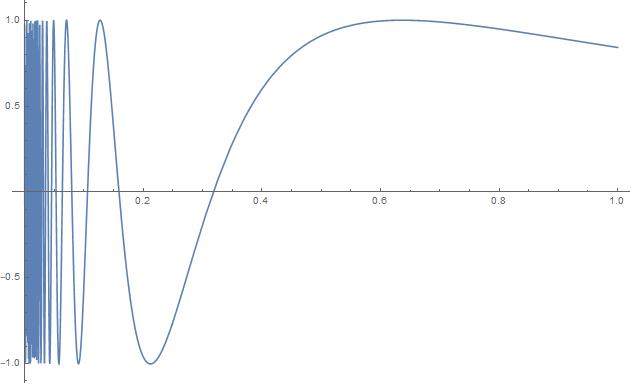
\includegraphics[scale=0.3]{Images/Top_sin.jpg}
    \caption{The topologists' sine curve}
    \label{tsine}
\end{figure}
The set is connected, since every point on the y-axis is a limit point of the curve. However, there is no continuous path connecting the y-axis to the rest of the curve, because $\sin(1/x)$ itself is not continuous.

\begin{xca}
\begin{enumerate}
    \item Show that the $n$-dimensional sphere $S^n$ (defined as the unit sphere in $\mathbb{R}^{n+1}$ with the subset topology) is path-connected.
    \item Show that $\mathbb{Q}\subset\mathbb{R}$ is not connected.
    \item Show that the product of two path-connected spaces is path-connected.
\end{enumerate}
\end{xca}


\begin{defn}[Covering]
A collection of subsets of a topological space $X$ is said to cover $X$ if the union of these subsets equals $X$. If the subsets are all open (closed), the covering is said to be open (closed).
\end{defn}

\PRLsep

\begin{defn}[Compact Space]\index{Compact space}
A space $X$ is called compact if every open cover of $X$ contains a finite subcollection that also covers $X$.
\end{defn}

\begin{defn}[Compact Subset]
A subset $A\subset X$ is called compact if it is compact in the subspace topology.
\end{defn}

\begin{prop}
If $Y_i\subset X$, $i = 1,\dots, m$ are compact subsets, then their union $\bigcup_{i=1}^m Y_i$ is also compact.
\end{prop}
\begin{proof}
Exercise.
\end{proof}

\begin{thm}[Compactness is a topological invariant]
The image $f(X)$ of a compact space $X$ under a continuous map $f\in C(X,Y)$ is compact.
\end{thm}
\begin{proof}
Exercise.
\end{proof}

\begin{xca}
\begin{enumerate}
    \item Show that the product of two connected spaces is connected. \emph{Hint:} first show that the union of any number of pairwise overlapping connected subspaces (i.e.\ subsets endowed with the subspace topology) of a space is also connected; then, write $X\times Y$ as the union of ``crosses'' $(\{x\}\times Y)\cup (X\times \{y\})$ that pairwise overlap and are connected only if $X$ and $Y$ are.
    \item Show that the product of two path-connected spaces is path-connected.
    \item Show that the product of two compact spaces is compact. \emph{Hint:} \cite{compact.proof}.
\end{enumerate}
\end{xca}


\begin{defn}[Classes of continuous maps]\index{Open map}\index{Closed map}\index{Proper map}
A map $f:X\to Y$ (not necessarily continuous) is called
\begin{enumerate}
    \item \emph{open} if the image of every open subset of $X$ is open in $Y$;
    \item \emph{closed} if the image of every closed subset of $X$ is closed in $Y$;
    \item \emph{proper} if it is continuous and the preimage of any compact subset of $Y$ is compact in $X$;
\end{enumerate}
\end{defn}

\begin{xca}
Show that the image of any proper map $f:\mathbb{R}^m\to\mathbb{R}^n$ is closed.
\end{xca}

\subsection{Metric Spaces}

\begin{defn}[Metric spaces]\index{Metric space}\index{Metric}
A \emph{metric space} is a set $X$ with a \emph{metric} $\rho:X\times X\rightarrow \mathbb{R}$ that obeys the following conditions for any $x,y,z\in X$
\begin{enumerate}
    \item \emph{Non-negativity}: $\rho(x,y)\ge 0$; \emph{non-degeneracy:} $\rho(x,y)=0$ iff $x=y$.
    \item \emph{Symmetry}: $\rho(x,y) = \rho(y,x)$.
    \item \emph{Triangle Inequality}: $\rho(x,y) + \rho(y,z) \ge \rho(x,z)$.
\end{enumerate}
\end{defn}

\begin{defn}[Metric maps]
A \emph{metric map} between two metric spaces $(X,\rho_X)$ and $(Y,\rho_Y)$ is a continuous map $f\in C(X,Y)$ such that $\rho_Y (f(x_1),f(x_2))\leq \rho_X (x_1,x_2)$. The category $\mathsf{Met}$ is defined as the category of metric spaces with metric maps for morphisms.
\end{defn}

\begin{defn}[Open Ball]
An \emph{open ball} $B_r(x)$ of radius $r$ around a point $x$ in a metric space $(X,\rho)$ is defined as
\begin{equation}
    B_r(x) = \{ y\in X ~|~ \rho(y,x)< r \}
\end{equation}
\end{defn}

\begin{defn}[Metric Topology]
The metric topology induced by a metric on a set is the topology generated by basis elements that are open balls $B_r(x)$ for all $x\in X$ and $r>0$. 
\end{defn}
\begin{rem}
Equivalently, by Proposition \ref{characterization of topology using basis}, a set $M$ is open in the metric topology iff for any $x\in M$ there exists a radius $r>0$ such that $B_r(x)\subset M$. In the metric topology, $\rho:X\times X\to \mathbb R$ is automatically continuous.
\end{rem}
\begin{prop}
If a metric space $(X,\rho)$ is separable, it has a countable base.
\end{prop}
\begin{proof}
Exercise. \emph{Hint}: consider balls of rational radius about every point of the dense subset.
\end{proof}

\begin{defn}[Limit of a Sequence]
A sequence of points $\{x_n\}$ in a metric space $X$ is said to \emph{converge} if there exists a point $x\in X$ such that for any $\epsilon >0$, there exists an $N\in \mathbb{N}$ such that
\begin{equation}
    \forall ~ n>N,\; \rho(x_n,x) < \epsilon.
\end{equation}
The point $x$ is called the limit of the sequence.
\end{defn}
Note that the limit of a sequence is unique by the first axiom of the metric. One can also define the limit point of a subset of a general topological space as follows:
\begin{defn}[Limit Point]
If $A$ is a subset of a topological space, a point $x\in X$ is said to be a limit point of $A$ if every open neighbourhood of $x$ intersects $A$ in some point other than $x$.
\end{defn}

In metric spaces, limit points are equivalent to limits of sequences, i.e., for every limit point $x$ of a subset $A$, there exists a sequence of points in $A$ that converges to $x$. Conversely, for any convergent sequence of points in $A$, the limit of the sequence is a limit point of $A$.

\begin{prop}
For a metric space $X$ equipped with the metric topology, the closure $\xoverline{A}$ of a subset $A\subset X$ is equal to the set of limit points of $A$.
\end{prop}
\begin{proof}
Exercise.
\end{proof}

\begin{prop}
For two metric spaces $(X,\rho)$ and $(Y,\rho')$ and a map $f:X\rightarrow Y$ such that $f(x)=y$, the following are equivalent
\begin{enumerate}
    \item $f$ is continuous at $x$.
    \item For any convergent sequence $x_n\rightarrow x$, the image is also convergent with $f(x_n)\rightarrow y$.
    \item For every $\epsilon>0$, there exists $\delta>0$ such that $\rho(x,z)<\delta \implies \rho'(f(x)=y, f(z))<\epsilon$.
\end{enumerate}
\end{prop}
\begin{proof}
Exercise.
\end{proof}

\begin{defn}[Isometry]\index{Isometry}
An isometry between two metric spaces is a bijective map $f:X\rightarrow Y$ that preserves distances, i.e.,
\begin{equation}
    \rho_X(x,y) = \rho_Y(f(x), f(y)).
\end{equation}
\end{defn}

\begin{prop}
If $f:X\rightarrow Y$ is an isometry, it is also a homeomorphism.
\end{prop}
\begin{proof}
Exercise.
\end{proof}

\begin{defn}[Equivalent metrics]\index{Metric!equivalence of}
Two metrics $\rho_1,\rho_2$ on a topological space $X$ are called equivalent if for any $x\in X$ and any $r>0$, there exist radii $r',r''>0$ such that $B^{(1)}_{r'}(x)\subset B^{(2)}_{r}(x)$ and $B^{(2)}_{r''}(x)\subset B^{(1)}_{r}(x)$ (here, $B^{(i)}$ denotes an open ball defined by the metric $\rho_i$).
\end{defn}

\begin{thm}
Two metrics on the same space are equivalent iff they induce the same topology.
\end{thm}
\begin{proof}
Exercise.
\end{proof}

\begin{defn}[Cauchy sequence]\index{Cauchy sequence}
A sequence $(x_n)$ of points of a metric space $(X,\rho)$ is called a Cauchy sequence if for any $\epsilon>0$ there exists $N\in\mathbb{N}$ such that $\forall n,m\geq N$, $\rho(x_n,x_m)<\epsilon$.
\end{defn}

\begin{defn}[Completeness]\index{Complete metric space}
A metric space $(X,\rho)$ is called complete if every Cauchy sequence $(x_n)$ in it has a limit $x_\infty\in X$.
\end{defn}

\begin{thm}[Cantor's intersection theorem]
Let $(X,\rho)$ be a complete metric space and let $C_n$ be a sequence of closed nested subsets $C_{n+1}\subset C_n$ whose diameters tend to zero, $\mathrm{diam}\,C_n=\sup_{x,y\in C_n} \rho(x,y) \to 0$. Then the intersection $\bigcap_{n=1}^\infty C_n$ consists of exactly one point.
\end{thm}

\begin{xca}
Consider $\mathbb{N}$ with the metric $\rho (n,m)=\lvert \frac 1 n-\frac 1 m\rvert$. Construct a sequence of balls $B_{r_k}(x_k)$ in this space such that $r_{k+1}<r_k$, $B_{r_{k+1}}(x_{k+1})\subset B_{r_k}(x_k)$, but the intersection of all these balls is empty.
\end{xca}
\begin{defn}[Normed vector space]\index{Normed vector space}\index{Norm}
A normed vector space is a vector space $V$ over a subfield of $\mathbb{C}$ with a function (called the norm) $\lVert \cdot \rVert: V\to \mathbb R_+$ such that for all $x,y\in V$:
\begin{enumerate}
    \item $\lVert x\rVert\geq 0$, and $\lVert x\rVert= 0$ iff $x=0$;
    \item $\lVert \alpha  x\rVert=\lvert \alpha \rvert \lVert x\rVert$ for any scalar (element of the structure field) $\alpha$;
    \item $\lVert x+y\rVert\leq \lVert x\rVert+\lVert y\rVert$.
\end{enumerate}
Every normed vector space has a naturally induced metric $\rho (x,y)=\lVert x-y\rVert$. In the corresponding induced topology, the norm is automatically continuous.

\end{defn}
\begin{defn}[Equivalent norms]\index{Norm!equivalence of}
Two norms $\lVert\cdot \rVert_1,\lVert\cdot \rVert_2 $ on a vector space $X$ are called equivalent if there are (universal) constants $\alpha,\beta >0$ such that for all $x\in X$ we have $\alpha \lVert x \rVert_1\leq \lVert x \rVert_2 \leq \beta \lVert x \rVert_1$.
\end{defn}
Notice how this condition is much stronger than just the equivalence of the induced metrics, since $\alpha$ and $\beta$ are required to be universal constants for all $x$.

\begin{thm}
Two norms on a vector space $X$ are equivalent iff they induce the same topology.
\end{thm}
\begin{proof}
Exercise.
\end{proof}

\subsection{Separation Axioms} \label{Separation Axioms}

We saw that every metric space has a canonical topology associated with it. A natural question to ask is whether the converse is true. Given a topological space, when can we define a metric on it such that the topology coincides with the metric topology? Clearly, a metric space has more structure than a topological space. In order to add more structure to topological spaces, we define the following axioms

\begin{defn}[Separation Axioms]\index{Separation axioms}
For a topological space $X$ with arbitrary points $x$ and $y$ and arbitrary disjoint closed sets $F$ and $G$, we define the following axioms:
\begin{enumerate}
    \item $T_1$: There exists an open neighbourhood $U$ of $x$ that doesn't include $y$, and an open neighbourhood $V$ of $y$ that doesn't include $x$, i.e., $x$ and $y$ are \emph{separated}.
    \item $T_2$ (\emph{Hausdorff}): There exist disjoint open neighbourhoods $U$ of $x$ and $V$ of $y$, i.e., $x$ and $y$ are \emph{separated by neighbourhoods}.
    \item $T_3$: There exist disjoint open neighbourhoods $U$ of $x$ and $V$ of $F$.
    \item \emph{Regular}: $X$ is both $T_1$ and $T_3$.
    \item $T_4$: There exist disjoint open neighbourhoods $U$ of $F$ and $V$ of $G$.
    \item \emph{Normal}: $X$ is both $T_1$ and $T_4$.
\end{enumerate}
\end{defn}

\begin{prop}
The following results demonstrate how each axiom adds additional structure to the space:
\begin{enumerate}
    \item $T_1 \implies$ All finite sets are closed;
    \item $T_2\implies T_1$;
    \item Regular $\implies$ Hausdorff;
    \item Normal $\implies$ Regular.
\end{enumerate}
\end{prop}

\begin{example}
The category $\mathsf{Hausd}$ of Hausdorff spaces is a full subcategory of $\mathsf{Top}$.
\end{example}

\begin{thm}[Urysohn Lemma]\index{Urysohn lemma}
A space $X$ is normal iff for any two disjoint closed subsets $A$ and $B$ there exists a continuous function
\begin{equation}
f\in C(X,[0,1]) ~\text{such that}~ \restr{f}{A} = 0, \restr{f}{B} = 1.
\end{equation}
\end{thm}

\begin{thm}
All metric spaces are normal.
\end{thm}
\begin{proof}
Exercise.
\end{proof}

\begin{thm}[Urysohn]
A normal space with a countable base is \emph{metrizable}, i.e., we can construct a canonical metric whose induced topology coincides with the topology of the space.
\end{thm}

\begin{prop}
If $X$ is Hausdorff, every compact subset of $X$ is closed.
\end{prop}
\begin{proof}
Exercise. \emph{Hint:} prove that the complement of the compact set is open by using Proposition \ref{open iff contains neighborhoods}.
\end{proof}

\begin{prop}
Every compact Hausdorff space is normal.
\end{prop}
\begin{proof}
Exercise.
\end{proof}

\begin{thm}[Heyne-Borel]\index{Heyne-Borel theorem}
In Euclidean space $\mathbb{R}^n$, a subset is compact iff it is closed and bounded.
\end{thm}

The following theorem is one of the most fundamental theorems in functional analysis, and it essentially characterizes compact subsets of the set of continuous functions defined on a compact subset of $\mathbb{R}^n$. We state it simply as an example of usage of the above topological terminology.
\begin{thm}[Arzel\`a-Ascoli]
Let $X$ be a compact Hausdorff space. A subset $F$ of the space $C(X,\mathbb{R})$ of continuous real-valued functions on $X$ is relatively compact (i.e.\ its closure is compact) in the topology given by the sup-norm $\lVert f\rVert=\sup_X \vert f\rvert$ iff it is equicontinuous (i.e.\ all elements $f\in F$ are uniformly continuous functions and the $\delta$ in the definition of uniform continuity is universal for all $f\in F$) and pointwise bounded (i.e.\ for every $x\in X$ the set $\{f(x)\}_{f\in F}$ is bounded).
\end{thm}

\subsection{Homotopy}\label{sec.homotopy}
\begin{defn}[Homotopic maps]\index{Homotopy} Two continuous maps $f_0,f_1\in C(X, Y)$ are called homotopic (we often write $f\sim g$) if there exists a continuous map, called homotopy, $F\in C([0,1]\times X,Y)$ such that $F(0,x)=f_0(x)$ and $F(1,x)=f_1(x)$. Here, $[0,1]$ has the standard topology.
\end{defn}
\begin{prop}
Homotopy is an equivalence relation on $C(X,Y)$. (The set of all homotopy classes of continuous maps from $X$ to $Y$ is denoted by $[X,Y]$. This set defines the morphisms in the (naive) homotopy category $\mathsf{hTop}$.)
\end{prop}
\begin{proof}
Exercise.
\end{proof}

The first argument of $F(t,x)$ is essentially ``time'', and $F(t,\cdot)$ continuously interpolates between $f_0$ and $f_1$ as time goes from 0 to 1. In topology, homotopy is synonymous with the phrase ``continuous deformation''.

\begin{defn}[Homotopy equivalence of spaces]\index{Homotopy equivalence}
Two topological spaces $X$ and $Y$ are called homotopy equivalent if there exist two continuous maps $f\in C(X,Y)$, $g\in C(Y,X)$ such that $g\circ f\sim \id_X$ and $f\circ g\sim \id_Y$. We write $X\simeq Y$.
\end{defn}

\begin{example}
\begin{enumerate}
    \item $S^1\times\mathbb{R}\simeq S^1\simeq M$, where $M$ is the M\"obius band.
    \item $\mathbb{R}^n\setminus{0}\simeq S^{n-1}$.
    \item More generally, two spaces $X,Y$ are homotopy equivalent iff they are both deformation retracts of the same space $Z$. That is, there needs to exist $A_X\subset Z$ such that $A_x\cong X$ and there exists a continuous map $F\in C([0,1]\times Z,Z)$ such that $F_X(0,z)=z$, $F_X(1,z)\in A$ and $F_X(t,a)=a$ for any $z\in Z$, $t\in [0,1]$ and $a\in A_x$. Similarly, there needs to exist $A_Y\subset Y$ homeomorphic to $Y$ that is a deformation retract of $Z$.
\end{enumerate}
\end{example}

\begin{defn}[Contractible space]\index{Contractible space}
A space $X$ is called contractible if it is homotopy equivalent to the one-point space, i.e.\ there exists a point $x_0\in X$ such that the constant map $f(x)=x_0$ is homotopic to the identity, $f\sim \id_X$. This property is in fact independent of $x_0$.
\end{defn}
\begin{prop}
Any contractible space is path-connected.
\end{prop}
\begin{proof}
Exercise. \emph{Hint:} consider paths traced out by $F(t,x)$ for fixed $x$'s.
\end{proof}
\begin{example}
\begin{enumerate}
    \item $\mathbb{R}^n$, $B^n$, $(0,1)^n$ are all contractible via, say, $F(t,x)=tx$ (they are also all homeomorphic to each other).
    \item Any two continuous functions $f,g:\mathbb{R}\to\mathbb{R}$ are homotopic via homotopy $F(t,x)=tg(x)+(1-t)f(x)$.
\end{enumerate}
\end{example}
\begin{xca}
Show that if $Y$ is contractible, then any two maps $f,g\in C(X,Y)$ are homotopic. This is a generalization of the above example for $X=Y=\mathbb{R}$.
\end{xca}
\begin{thm}[Brower]
The sphere $S^n$ is not contractible.
\end{thm}
\begin{proof}
    There is a plethora of different ways to prove this theorem, from pure analytical to algebraic. We will delay the proof until we compute the homology groups of the spheres in Part \ref{Part II} and observe that they differ from those of a contractible space (and homology groups are topological invariants).
\end{proof}
\begin{thm}[Brower's fixed point theorem]\index{Brower fixed point theorem}
Any continuous map $f\in C\left(\xoverline{B^n},\xoverline{B^n}\right)$  from the closed unit ball to itself has at least one fixed point ($x_0$ such that $f(x_0)=x_0$).
\end{thm}
\begin{proof}
For $n=1$ this is clear. For $n\geq 2$, suppose $f(x)\neq x$ for all $x$. Then we can define $h(x)$ as the point of intersection of the ray $[f(x),x)$ with the boundary of the ball. Then $F(t,x)=h(tx)$ is a contracting homotopy, which contradicts the last theorem.
\end{proof}
\begin{rem}
These two theorems are in fact equivalent. The fixed point theorem can be proven purely analytically, and the contractibility theorem will follow. The simplest modern proof of non-contractibility of $S^n$ is based on homology.
\end{rem}

\begin{defn}[Loops, Based homotopy]\index{Loop}
Let $X$ be a path-connected topological space, pick a ``base point'' $x_0\in X$, and consider the set of all \emph{loops} in $X$ based at $x_0$, i.e.\ paths $\gamma\in C([0,1], X)$ such that $\gamma(0)=\gamma(1)=x_0$. A based homotopy between two such loops is a homotopy $F\in C([0,1]\times[0,1],X)$ such that $F(\cdot,0)=F(\cdot,1)=x_0$. Based homotopy is an equivalence relation on the set of based loops.
\end{defn}

\begin{defn}[Fundamental/Poincar\'e group]\index{Fundamental group}
The fundamental group $\pi_1(X,x_0)$ of a path-connected space $X$ with a base point $x_0$ is defined as the set $\{ [\gamma]\}$ of based homotopy classes of based loops with the inversion operation given by $[\gamma(t)]^{-1}=[\gamma(1-t)]$ and the multiplication operation 
\[
[\gamma_1(t)]\circ [\gamma_2(t)]=\left[ \begin{cases} \gamma_1(2t), & t\in[0,1/2], \\ \gamma_2(2t-1), & t\in(1/2,1] \end{cases}\right].\label{pi1 group op}
\]
The unit element is given by the equivalence class of the ``constant loop'' $\gamma(t)\equiv x_0$. If $X$ is not path-connected, then $\pi_1(X,x_0)$ is defined as the fundamental group of the path-connected component containing $x_0$.
\end{defn}

\begin{xca}
Check that this definition is consistent, i.e.\ the homotopy classes on the right-hand sides don't depend on the choices of representatives of the classes on the left.
\end{xca}
\begin{defn}[Simple-connectedness]\index{Simply connected space}
A path-connected space $X$ is called simply connected if its fundamental group is trivial, $\pi_1(X,x_0)=\{e\}$.
\end{defn}

\begin{xca}
Show that contractible spaces are simply connected.
\end{xca}

\begin{defn}[Alternative approach]
Recall that the category $\mathsf{Top}_\bullet$ consists of ``pointed topological spaces'' with chosen base points and morphisms that are continuous maps mapping base point to base point. Take the circle $S^1$ and pick a point $\bullet$ in it. Then one can redefine based loops as morphisms between two pointed topological spaces $\gamma\in C((S^1,\bullet),(X,x_0))$. Based homotopy in the definition of $\pi_1$ can then be replaced by just homotopy of loops as maps defined on $S^1$.   Thus, as a set, $\pi_1(X)=[S^1,X]_\bullet$ (group of homotopy classes of pointed maps).
\end{defn}
\begin{prop}\label{prop computing pi1}
\begin{enumerate}
    \item $\pi_1$ is a covariant functor $\pi_1:\mathsf{Top}_\bullet\to \mathsf{Gr}$.
    \item For a path-connected space, fundamental groups with different base points are isomorphic, so we usually abuse the notation by writing $\pi_n(X)$.
    \item For any number of path-connected spaces, $\pi_n(\prod_\alpha X_\alpha)\cong \prod_\alpha \pi_n(X_\alpha)$.
    \item For a pair of path-connected spaces, $\pi_1(X\lor Y)\cong \pi_1(X)\ast \pi_1(Y)$, where $\lor$ is the wedge sum\index{Wedge sum of pointed spaces} (disjoint union with base points identified) and $\ast$ is the free product of groups. As a result, $\pi_1$ is a functor that preserves categorical products \emph{and} coproducts.
\end{enumerate}
\end{prop}
\begin{proof}
Exercise.
\end{proof}
\begin{defn}[Homotopy groups]\index{Homotopy groups}
Pick the base points $\bullet\in S^n$ and $x_0\in X$. The set of homotopy classes of maps $\gamma:S^n\to X$ such that $\gamma(\bullet)=x_0$ forms the $n$-th homotopy group $\pi_n(X,x_0)=[S^n,X]_\bullet$. For two such maps, define their product by first mapping $S^n$ onto the wedge sum $S^n\lor S^n$ via contracting an arbitrarily chosen equator (which is homeomorphic to $S^{n-1}$) into one point, then apply $\gamma_1$ and $\gamma_2$ to the two hemispheres respectively, making the equator point the base point for them.

For $n=0$, $\pi_0(X)$ is defined as the set of path-connected components of $X$ (which is also the set of homotopy classes of pointed maps $S^0\to X$) but does not have a natural group structure.
\end{defn}
\begin{xca}
\begin{enumerate}
    \item The above definition is consistent and the resulting homotopy classes don't in fact depend on the choice of an equator. In fact, in natural terms, this group operation is exactly the coproduct on the category of pointed spaces, given by the wedge sum $\gamma_1\lor\gamma_2:S^n\lor S^n\to X$ (a.k.a. \emph{concatenation}).
    \item All homotopy groups for different $x_0$ are isomorphic.
\end{enumerate}

\end{xca}
\begin{thm}
Homotopy groups $\pi_n$, $n\geq 1$, are homotopy invariants, i.e.\ If $X\simeq Y$ are two homotopy equivalent connected spaces, then $\pi_n(X)\cong\pi_n(Y)$.
\end{thm}
\begin{proof}
Exercise. Also see \cite{Hatcher}.
\end{proof}

\begin{example}
\begin{enumerate}
    \item The shape $\ominus$ is a deformation retract of the figure 8, which itself is just the wedge sum $S^1\vee S^1$, so their fundamental groups are all $\mathbb{Z}\ast\mathbb{Z}$.
    \item The last example can be generalized to compute $\pi_1$ of an arbitrary connected graph. The result is just the free group generated by the set of (elementary) loops in the graph. More precisely, the number of generators equals the number of all edges of the graph minus the number of edges in a maximal spanning tree of the graph (i.e.\ a maximal subgraph without loops).
\end{enumerate}
\end{example}

\begin{thm}
For $n\geq 2$, all groups $\pi_n(X,x_0)$ are Abelian.
\end{thm}
\begin{proof}
See \cite{Hatcher}.
\end{proof}

\begin{comment}
\PRLsep
\begin{center}
  {\red Lecture 4 on 30 Nov 2018 ended here}
\end{center}
\end{comment}



\section{Manifolds}

\subsection{Topological Manifolds}
\begin{defn}[Locally Euclidean Space]\index{Locally Euclidean Space}
A topological space $X$ is locally $n$-dimensional Euclidean if every $x\in X$ has an open neighborhood homeomorphic to the open $n$-dimensional ball, $U_x\cong B^n$. 
\end{defn}
\begin{defn}[Second-countability]\index{Second countable space}
A topological space is called second countable if it has a countable basis of topology.
\end{defn}
\begin{defn}[Paracompactness]\index{Paracompact space}
\begin{enumerate}
    \item A collection of subsets $A_\alpha, \alpha \in I,$ of $X$ is called locally finite if every $x\in X$ has an open neighborhood $U_x$ such that $U_x\cap A_\alpha \neq \varnothing$ only for a finite number of $\alpha$'s. If all $A_\alpha$'s are open, this is the same as $x$ being an element of only finitely many of them.
    \item Given an open cover $\{U_\alpha\}$ (i.e.\ a collection of open sets such that $\bigcup_\alpha U_\alpha=X$), a refinement of it is a covering $\{V_\beta \}$ such that $\forall \beta \;\exists \alpha: V_\beta \subset U_\alpha $.
    \item $X$ is called paracompact if every open cover of $X$ admits an open, locally finite refinement.
\end{enumerate}
\end{defn}
\begin{defn}[Topological manifold]\index{Manifold!topological}
A topological manifold is a second countable, Hausdorff, locally Euclidean space.
\end{defn}
The following proposition is the reason why second countability is often substituted with paracompactness in the definition of manifolds.
\begin{prop}
All topological manifolds are paracompact (and locally compact).
\end{prop}
\begin{proof}
See \cite[Thm. 1.15]{Lee}
\end{proof}
\begin{defn}[Charts]\index{Chart}
Let $X$ be an $n$-dimensional topological manifold. A \emph{chart} on it is a pair $(U,\varphi)$, where $U\subset X$ is an open set and $\varphi:U\to \mathbb{R}^n$ is a continuous map (called the chart map) that is also a homeomorphism onto its image $\wh{U}=\varphi (U)$, i.e.\ $U\cong \varphi(U)=\wh{U}$. The chart is called a \emph{coordinate ball} if $\wh U$ is a ball in $\mathbb{R}^n$. The values of $\varphi$ are called \emph{coordinates} of the corresponding points on $X$.
\end{defn}
\begin{rem}
Since $X$ is locally Euclidean, every point $x$ automatically has a chart $(U_x,\varphi)$ around it. In particular, every manifold has an open cover by charts $(U_\alpha,\varphi_\alpha)$.
\end{rem}

\begin{thm} All topological manifolds have the following properties.
\begin{enumerate}
    \item There is a countable basis consisting of coordinate balls (it can also be made locally finite and every ball can be made precompact)
    \item Local compactness.
    \item Local path-connectedness (i.e.\ every point has a path-connected neighborhood).
    \item At most countably many connected components, each open and a topological manifold of its own.
    \item The fundamental group $\pi_1(X)$ is at most countable.
\end{enumerate}
\end{thm}
\begin{proof}
1,2) Pick an open cover by charts $\{U_\alpha\}$. Each $U_\alpha $ can be covered by countably many coordinate balls $V_{\alpha_i}$ because $\wh{U}_\alpha$ can be covered by countably many balls in $\mathbb{R}^n$. By second countability, there is a countable subcovering and basis $\{V_\beta\}$. Fixing a chart $U$ and covering it by coordinate balls $V_\alpha$, we have that $\xoverline{V}_\beta$ is compact in $U$ (because it's homeo to a closed ball), therefore closed in $X$ by Hausdorffness. Therefore it's also compact in $X$, i.e.\ $V_\beta$'s are precompact. The covering can also be made locally finite: let $\{K_i\}_{i=1}^\infty$ be an exhaustion of $M$ by compact sets (i.e.\ $\bigcup_i K_i=M$; we will prove the existence in Prop. \ref{prop.exhaustion}). After picking out a finite subcovering of every compact ``stripe'' $K_{i+1}\setminus \Int K_{i}$ by charts that are small enough to fit within the wider open ``stripe'' $\Int K_{i+2}\setminus K_{i-1}$ (possible because all charts still form a basis), we end up with a locally finite covering (since every point of the manifold is contained only in 3 of the open stripes).

3) Obvious because balls are.

4) 2nd countability implies countable components. The rest is obvious.

5) See \cite[Thm 1.16]{Lee}.
\end{proof}

\begin{lem}
Locally path-connected and connected $\Leftrightarrow$ path-connected.
\end{lem}
\begin{proof}
The reverse direction is obvious. In the forward direction, introduce the set $C=\{q:q\text{ is connected with }p\}$  for some fixed $p\in X$. We will prove that $C$ is clopen and therefore equal to $X$.

$C$ is open because $X$ is locally path-connected.
$C$ is closed because for any $z\in\xoverline{C}$ there is a path-connected neighborhood $U_z$, thus $U_z\cap C\neq \varnothing$, and $z\in C$. Therefore $\xoverline C=C$. 
But $X$ is connected, and $C$ is clearly not empty, therefore $C=X$, and lastly $C$ is path-connected by definition.
\end{proof}
\begin{cor}
For manifolds, connectedness is equivalent to path-connectedness. In particular, connected components of manifolds are path-connected.
\end{cor}

\begin{example}
\begin{enumerate}
    \item Any open set in $\mathbb{R}^n$ is a manifold.
    \item $S^n$ is a manifold because it can be covered by finitely many charts $(U_i,\varphi_i)$, where $U_i$ is an open hemisphere whose ``equator'' lies on one of the coordinate hyperplanes, and $\varphi_i$ is simply the orthogonal projection to that hyperplane.
    \item An $n$-dimensional torus $T^n=(S^1)^{\times n}$ is a manifold.
    \item The figure eight, 8, as a subset of $\mathbb{R}^2$, is not a manifold, because its center doesn't have a neighborhood homeomorphic to an interval.
    \item Matrices $\Mat(n,\mathbb{R})$ form an $n^2$-dimensional manifold (isomorphic to $\mathbb{R}^{n^2}$). So do invertible matrices $\GL(n,\mathbb{R})$ (being an open subset in $\mathbb{R}^{n^2}$) and all other classical matrix groups.
\end{enumerate}
\end{example}

\subsection{Smooth Structures}
\begin{defn}[Atlas]\index{Atlas!topological}
An atlas $\mathcal{A}$ for a topological manifold $M$ is a collection of continuous charts $\{(U_\alpha,\varphi_\alpha)\}$, $\varphi_\alpha:U_\alpha\to \wh{U}_\alpha \subset \mathbb{R}^n$ such that $\bigcup_\alpha U_\alpha =M$.
\end{defn}
Throughout these notes we also adopt the notation where for any atlas as above, $U_{\alpha\beta}=U_\alpha \cap U_\beta$, $U_{\alpha\beta\gamma}=U_\alpha \cap U_\beta \cap U_\gamma$, etc.

\begin{defn}[Smooth atlas]\index{Atlas!smooth}
An atlas is called smooth (or of class $C^k$ or $C^\omega$) if all of the \emph{transition functions} $\varphi_{\beta\alpha}=\varphi_\beta\circ\varphi_\alpha^{-1}:\varphi_\alpha(U_{\alpha\beta})\to\varphi_\beta(U_{\alpha\beta})$ are smooth/$C^\infty$ (of class $C^k$, or real analytic, respectively) in the sense of multivariable calculus on $\mathbb{R}^n$.
\end{defn}
\begin{defn}[Equivalent atlases]\index{Atlas!equivalence of}
Two atlases $\mathcal{A}_1$ and $\mathcal{A}_2$ are called equivalent, or compatible, if $\mathcal{A}_1\cup\mathcal{A}_2$ is still an atlas of the same smoothness class.
\end{defn}
\begin{defn}[Differentiable structure]\index{Differentiable structure}\index{Smooth structure}
A smooth ($C^k$, analytic) structure on a topological manifold $M$ is an equivalence class $[\mathcal{A}]$ of smooth (respectively, $C^k$, $C^\omega$) atlases on it. 
\end{defn}
\begin{defn}[Smooth manifold]\index{Manifold!smooth}
A smooth manifold is a pair $(M,[\mathcal{A}])$ consisting of a topological manifold and a smooth structure.
\end{defn}
\begin{example}
\begin{enumerate}
    \item Let $\psi:\mathbb{R}\to\mathbb{R}$ be $\psi(x)=x^3$. Then $\{(\mathbb{R},\psi)\}$ is an atlas that defines a smooth structure on $\mathbb{R}$. It is not smoothly compatible with the standard smooth structure given by the chart map $\varphi(x)=x$, because the transition function $\varphi\circ \psi^{-1}(x)=x^{1/3}$ is not smooth. Therefore $\mathbb{R}$ has many (in fact, infinitely many) different smooth structures.
    \item Any real or complex vector space is automatically a smooth manifold.
    \item Spaces of matrices, classical groups, spheres... are all smooth manifolds with their standard structures.
    \item Not every topological manifold admits a smooth structure, although examples are pretty difficult to construct. On the other hand, any $C^1$ manifold admits a compatible (in the $C^1$ sense) smooth structure, which is unique up to diffeomorphism (see below). This is why even mathematicians are mostly happy working with just either topological or immediately smooth/analytic manifolds. Interestingly, all topological manifolds in dimensions 1,2, and 3 admit unique (up to diffeo) smooth structures.
    \item All Lie groups (defined as smooth manifolds with a group structure in which multiplication and inversion are smooth maps) in fact support a unique (up to diffeo) $C^\omega$ structure. This is an immediate consequence of the convergence of the Baker-Campbell-Hausdorff series.
\end{enumerate}
\end{example}

From now on we work only with smooth manifolds, and use the word ``manifold''  to mean ``smooth manifold''.
\begin{defn}[Smooth maps]\index{Smooth map}
Let $M$ and $N$ be two manifolds with atlases $\{(U_\alpha,\varphi_\alpha)\}$ and $\{(V_\beta,\psi_\beta)\}$, respectively. A map $f:M\to N$ is called smooth if all of its \emph{local representatives} $f_{\beta\alpha}=\psi_\alpha\circ f\circ \varphi_\beta^{-1}:\wh{U}_\beta\to \wh{U}_\alpha$ are smooth. The set of all smooth maps between two manifolds is denoted by $C^\infty (M,N)$. When $N=\mathbb{R}$, we write $C^\infty(M)=C^\infty (M,\mathbb{R})$ for the space of ``smooth functions''. The category $\mathsf{Man}^\infty$ is the category of smooth manifolds with smooth maps for morphisms.
\end{defn}
\begin{xca}
Check that all chart maps in any atlas of a smooth manifold $M$ are smooth as maps from $M$ to the standard $\mathbb{R}^n$.
\end{xca}
\begin{rem}
The above exercise illustrates the general alternative approach to manifolds: instead of defining a smooth structure in terms of charts, we could describe it by specifying \emph{what smooth functions should be} by describing the subsets of the sets of local continuous functions $C(U_\alpha)$ that we want to be smooth (more precisely, one has to pick a subsheaf of the sheaf of continuous functions that is locally isomorphic to the sheaf of smooth functions on $\mathbb{R}^n$).
\end{rem}
\begin{defn}[Manifolds with boundaries]\index{Manifold!with boundaries/corners}
Let $\mathbb{R}_+^n$ be the closed upper half-space in $\mathbb{R}^n$ (i.e.\ $x^n\geq 0$). An $n$-dimensional manifold with boundaries is defined just like a smooth manifold, only now some of the chart maps can map to $\mathbb{R}_+^n$. The smoothness of boundary transitions is characterized as follows: any function $\mathbb{R}_+^n\to \mathbb{R}_+^n$ is called smooth if it can be extended as a smooth function into an open neighborhood of $\mathbb{R}_+^n$. The set of points of $M$ that map to the boundary of $\mathbb{R}_+^n\subset \mathbb{R}^n$, i.e.\ the hyperplane $x^n=0$, is called the boundary $\partial M$. We also denote the interior by $\mathring M=M\setminus \partial M$.
\end{defn}
\begin{example}
$\sqrt{y}:\mathbb{R}_+\to\mathbb{R}$ is not smooth on $\mathbb{R}_+$ with the standard smooth structure. However, it can be taken to be the chart map defining a new smooth structure on $\mathbb{R}_+$, and in that new structure it'll become smooth, because its local representative will be the identity map.
\end{example}
\begin{rem}
Similarly, one can define \emph{manifolds with corners} using chart maps that can take values in quadrants, octants, and so on, of $\mathbb{R}^n$.
\end{rem}

\begin{defn}[Diffeomorphisms]\index{Diffeomorphism}
A smooth map $f:M\to N$ between manifolds is a called a diffeomorphism if it has a smooth inverse. They are the isomorphisms in $\mathsf{Man}^\infty$.
\end{defn}
\begin{prop}
\begin{enumerate}
    \item Diffeos are homeo and open.
    \item If $M$ and $N$ have boundaries and $f:M\to N$ is a diffeo, then $f(\partial M)=\partial N$ and $\restr{f}{\mathring M}: \mathring M\to \mathring N$ is a diffeo.
\end{enumerate}
\end{prop}
\begin{example}
\begin{enumerate}
    \item Different smooth structures can be diffeomorphic! Take $\mathbb{R}$ with the chart $\psi(x)=x^3$ that we considered earlier. It is diffeomorphic to the standard smooth structure given by the chart $\varphi(x)=x$, and the diffeomorphism is given by $\psi$ itself! Indeed, its local representative in the two charts is $\varphi\circ \psi \circ\psi^{-1}(x)=x$. In this manner one can show that there is only one smooth structure on $\bbR$ up to diffeomorphism.
    \item Historically the first manifolds to be found to support more than one non-diffeomorphic smooth structure were spheres, starting with $S^7$ which has 28 diffeomorphism classes of smooth structures. These smooth structures are now known as Milnor's \emph{exotic spheres}.
    \item $\mathbb{R}^n$ has only one smooth structure up to isomorphism for all $n\neq 4$. For $n=4$, it admits \emph{uncountably many} non-diffeomorphic structures. This makes the study of four-dimensional topological manifolds especially sophisticated, and there are still many very fundamental unsolved problems in four-dimensional topology \cite{smooth.structures}.
    \item In every dimension $n\geq 4$ there exist \emph{compact} topological manifolds that don't admit any compatible smooth structure.
\end{enumerate}
\end{example}

\begin{xca}
    Show that $S^1$ supports only one smooth structure up to diffeomorphism.
\end{xca}


\subsection{Partitions of unity}

First we note that on $\mathbb{R}^n$ there exist bump functions, i.e.\ for any point $x_0$ and any two radii $0<r_1<r_2$ there is a function $\eta\in C^\infty(\mathbb{R}^n)$ such that $\restr{\eta}{B_{r_1}(x_0)}=1$ and $\restr{\eta}{\mathbb{R}^n\setminus \overline{B_{r_2}}(x_0)}=0$.
\begin{xca}
Using the function $\int_a^x e^{\frac{1}{(x'-a)(b-x')}} \dd x'$ defined on $(a,b)$, construct a general bump function for $\mathbb{R}^n$.
\end{xca}

Now, any manifold $M$ can be covered by a locally finite collection of coordinate balls $(U_\alpha,\varphi_\alpha)$. Let $\eta_\alpha$ be a bump function that equals $0$ outside of the ball $\wh{U}_\alpha\subset \mathbb{R}^n$. Then define the smooth functions
\[f_\alpha =\begin{cases} \eta_\alpha\circ\varphi_\alpha, & \text{on }U_\alpha, \\ 0, & \text{on }M\setminus U_\alpha.\end{cases}\]
Finally, we normalize this collection of functions by defining
\[\chi_\alpha(x)=\frac{f_\alpha(x)}{\sum_\alpha f_\alpha (x).}\]
This expression is well-defined because the sum in the denominator is finite for every fixed $x$. These functions have the following properties:
\begin{enumerate}
    \item $\chi_\alpha\in C^\infty(M)$,
    \item $0\leq \chi_\alpha\leq 1$,
    \item $\supp \chi_\alpha\subset U_\alpha$,
    \item $\{\chi_\alpha\}$ is locally finite, i.e.\ only finitely many of them are non-zero at any given point $x\in M$,
    \item $\sum_\alpha \chi_\alpha (x)\equiv 1$.
\end{enumerate}

\begin{defn}[Partition of unity]\index{Partition of unity}
Any collection of functions satisfying the above list of properties is called a \gls{pou} subordinate to the open cover (not necessarily by coordinate balls) $\{U_\alpha\}$ of $M$.
\end{defn}
\begin{prop}
Any open cover of a smooth manifold admits a subordinate partition of unity.
\end{prop}
\begin{proof}
Any open cover has a locally finite refinement consisting of coordinate balls, which allows us to apply the construction above to the refinement. Notice that second countability is key to the existence of partitions of unity.
\end{proof}
\begin{thm}[Extension lemma]\label{extension lemma}\index{Extension lemma}
Let $A\subset M $ be a closed subset, and $f\in C^\infty(A,\mathbb{R}^k)$. Then for any open $U$ such that $A\subset U$, there exists an extension $\wt{f}\in C^\infty(M,\mathbb{R}^k)$: $\restr{\wt{f}}{A}=f$, such that $\supp \wt{f}\subset U$.
\end{thm}
\begin{proof}
Pick $p\in A$ and neighborhood $U_p\subset U$. Let $\wt{f}_p: U_p\to\mathbb{R}^k$ be a smooth extension of $f$ from $U_p\cap A$. It is guaranteed to exist for sufficiently small $U_p$ by definition of smoothness on closed subsets of $\mathbb{R}^n$ and smoothness of chart maps.

Then $\{U_p\}_{p\in A}\cup \{M\setminus A\}$ is an open cover of $M$. Let $\{\chi_p\}\cup\{\chi_0\}$ be a \gls{pou} subordinate to this covering (and $\chi_p=0$ inevitably for almost all $p$ so that the resulting collection is locally finite). Therefore $\chi_p\cdot \wt{f}_p:U_p\to\mathbb{R}^k$ are smooth and vanishing at the boundary of $U_p$, which allows us to extend them by zeros to smooth functions on all $M$. Finally, $\wt{f}=\sum_{p\in A} \chi_p \wt{f}_p$ is the extension we seek with support inside $U$.
\end{proof}
\begin{defn}[Exhaustion function]\index{Exhaustion}
A function $f\in C^\infty(M)$ is called an exhaustion function for $M$ if for every $c\in\mathbb{R}$ the preimage $f^{-1}((-\infty,c])$ is relatively compact (i.e.\ has compact closure in $M$).
\end{defn}
\begin{prop}\label{prop.exhaustion}
Every smooth manifold has an exhaustion function.
\end{prop}
\begin{proof}
Let $\{V_\alpha\}$ be a countable open cover by precompact sets and $\{\chi_\i\}_{i=1}^\infty$ a subordinate \gls{pou}. Define $f(x)=\sum_{n=1}^\infty n\cdot \chi_n(x)$. 

Clearly $f^{-1}((-\infty,c])\subset \bigcup_{i=1}^{[c]+1}\xoverline{V_i}$, which is a compact set.
\end{proof}

\subsection{Sard's Theorem}

In $\mathbb{R}^n$, a set $A$ is said to have\emph{ zero measure} if for any $\epsilon>0$ it can be covered by a collection of open balls $B_i$ such that the total volume of these balls is less than $\epsilon$.

\begin{defn}[Measure zero]
Even though there is no canonical way to measure volumes on manifolds, there is still a consistent notion of zero measure. Namely, a set $A\subset M$ has zero measure if all the sets $\varphi_\alpha(A\cap U_\alpha)$ are measure zero in $\mathbb{R}^n$ for an atlas $\{(U_\alpha,\varphi_\alpha)\}$.
\end{defn}

\begin{defn}[Rank of a map]\label{def.rank}\index{Rank of a map}
Let $f\in C^\infty (M^m,N^n)$ (superscripts here indicate the dimensions of the manifolds). We say that the rank of $f$ at $p\in M$ is $\rank_p f=r$ if there exist two local charts, $(U,\varphi)$ around $p \in M$ and $(V,\psi)$ around $f(p)\in N$, such that the local representative of $f$ in these charts is $\psi\circ f\circ\varphi^{-1}(x^1,\ldots,x^m)=(x^1,\ldots,x^r,\underbrace{0,\ldots,0}_{n-r})$.
\end{defn}

\begin{defn}[Critical and regular points/values]\index{Critical points/values}\index{Regular points/values}
$p\in M$ is said to be a critical point of $f\in C^\infty(M^m,N^n)$ if $\rank_p f<n$. In this case, $f(p)\in N$ is called a critical value of $f$. Otherwise, $p$ is a regular point, and a regular value is one all of whose preimages are regular points.
\end{defn}
\begin{thm}[Sard]\index{Sard theorem}
For any $f\in C^\infty(M,N)$ the set of critical values (also known in some contexts as the \emph{caustic}) of $f$ has measure zero in $N$.
\end{thm}
\begin{proof}
This theorem is essentially entirely local, i.e.\ it suffices to prove it for $M=\mathbb{R}^m$ and $N=\mathbb{R}^n$. See \cite[Thm 6.10]{Lee}.
\end{proof}

\subsection{Inverse Mapping Theorem (InMT) and Implicit Mapping Theorem (ImMT)}

In this section we just recall the statements of two basic theorems in multivariable calculus.
\begin{thm}[\Gls{inmt}]\label{InMT}
Let $U,V\subset\mathbb{R}^n$ be open and $f\in C^\infty(U,V)$. If the Jacobi matrix $\frac{\partial f^i}{\partial x^j} (a)$ is invertible for some $a\in U$, then there are neighborhoods $a\in U_a\subset U$ and $f(a)\in V_{f(a)}\subset V$ such that $\restr{f}{U_a}:U_a\to V_{f(a)}$ is a diffeomorphism.
\end{thm}
Meaning: any smooth map whose Jacobi matrix is non-singular at a point is locally a diffeomorphism around that point.

\begin{thm}[\Gls{immt}]\label{ImMT}
Let $U\subset \mathbb{R}^n\times \mathbb{R}^k$ be open, $(x,y)=(x^1,\ldots,x^n,y^1,\ldots,y^k)\in U$. Let $\Phi\in C^\infty(U,\mathbb{R}^k)$ and $\Phi(x,y)=c$. If the matrix $\left(\frac{\partial\Phi^i}{\partial y^j}(x,y)\right)_{i,j=1}^k$  is non-singular, then there are open neighborhoods $x\in V_x\subset \mathbb{R}^n$ and $y\in W_y\subset\mathbb{R}^k$ and a smooth map $f\in C^\infty (V_x,W_y)$ such that 
\[\forall\,(v,w)\in V_x\times W_y,\;\; \Phi (v,w)=c \Leftrightarrow w=f(v).\]
\end{thm}
Meaning: the equation $\Phi(x,y)=c$ can be locally solved for $y=y(x)$ if the matrix $\partial\Vec{\Phi}/\partial\Vec{y}$ is invertible.

\begin{comment}
\PRLsep
\begin{center}
  {\red Lecture 5 on 7 Dec 2018 ended here}
\end{center}
\end{comment}

\subsection{Tangent Spaces}
In $\mathbb{R}^n$, vectors don't have ``base points'' becase they can always be parallel transported to the origin. On a manifold, this is impossible, which is why there is a tangent space ``attached'' to every point $p\in M$. 
\begin{defn}[Tangent vector]\index{Tangent vector}\index{Vector}
Let $p\in M$. If $p\in \mathring M$, consider all curves $\gamma\in C^\infty((-1,1),M)$ such that $\gamma(0)=p$. If $p\in \partial M$, consider instead all curves with domains $(-1,0]$ or $[0,1)$. Introduce the equivalence relation $\gamma_1\sim \gamma_2$  iff $\restr{\frac{\dd}{\dd t}}{t=0}(\varphi_\alpha\circ \gamma_1)(t)=\restr{\frac{\dd}{\dd t}}{t=0}(\varphi_\alpha\circ \gamma_2)(t)$ for any chart $\varphi_\alpha$ around $p$. A tangent vector at $x$ is an equivalence class $[\gamma]_p$ of curves passing through $p$. The set of all tangent vectors at $p$ is denoted by $T_p M$.
\end{defn}

\begin{enumerate}
    \item $T_x M$ is imbued with the structure of a real vector space as follows:
    \begin{enumerate}
        \item $\lambda\cdot [\gamma(t)]_p\coloneqq [\gamma(\lambda t)]_p$ for $\lambda\in\mathbb{R}$.
        \item $[\gamma_1(t)]_p+[\gamma_2(t)]_p\coloneqq [\varphi_\alpha^{-1}(\varphi_\alpha(\gamma_1(t))+\varphi_\alpha(\gamma_2(t)))]_p.$
    \end{enumerate}
    \item We will show later that $\dim T_p M=\dim M$.
\end{enumerate}


\begin{defn}[Tangent vector, alternative def.]
$T_p M$ can be alternatively defined as the set of all \emph{derivations}\index{Derivation} at $p$, i.e.\ linear functionals $v:C^\infty(M)\to \mathbb{R}$ such that $v[f\cdot g]=f(p)v[g]+g(p)v[f]$. This is obviously a vector space. Notably, this definition doesn't need to be modified if $p\in\partial M$.
\end{defn}

\begin{prop}
The two definitions of tangent spaces given above are isomorphic as vector spaces.
\end{prop}
\begin{proof}
An explicit linear isomorphism between the two constructions is $[\gamma]_p\mapsto v[f]=\restr{\frac{\dd}{\dd t}}{t=0}f(\gamma(t))$ (this is called the \emph{directional derivative} along the tangent vector $[\gamma]_p$). 

All derivations on the algebra of smooth functions can be shown to be directional derivatives, which allows us to invert this mapping. Namely, for a chart map $\varphi_\alpha$, the $n$ numbers $v[\varphi_\alpha^i]$ are components of a vector $\wh{v}\in \mathbb{R}^n$. Now we can let $\wh{\gamma}(t)=\varphi_\alpha(p)+t\wh{v}$ and $\gamma(t)=\varphi_\alpha^{-1}(\wh{\gamma}(t))$. It is easy to show that this is a linear inverse to the above mapping.
\end{proof}


\begin{xca}
Check that the definition of a tangent vector and all of the following constructions are consistent, i.e.\ independent of the choices of charts $\varphi_\alpha$ or representatives $\gamma(t)$ of equivalence classes.
\end{xca}
\begin{defn}[Differential/push-forward]\index{Push-forward}
Let $F\in C^\infty(M,N)$ and $p\in M$. The push-forward of $F$ at $p$ is the linear map $D_p F=F_{\ast p}:T_p M\to T_{F(p)} N$ defined via \[F_{\ast p}([\gamma]_p)=[F\circ\gamma]_{F(p)},\] or equivalently \[F_{\ast p}(v)[f]=v[f\circ F]\] for any $f\in C^\infty (N)$.
\end{defn}

\begin{thm}\label{prop of push-forwards}
Consider smooth maps between manifolds $M\overset{f}{\to}N\overset{g}{\to}P$. Then
\begin{enumerate}
    \item $f_{\ast p}:T_x M\to T_{f(p)} N$ is linear;
    \item $(g\circ f)_{\ast p}=g_{\ast f(p)}\circ f_{\ast p}$ (chain rule);
    \item $(\id_M)_{\ast p}=\id_{T_p M}$;
    \item if $f$ is a local diffeo at $x$ then $f_{\ast p}$ is invertible and $(f_{\ast p})^{-1}=(f^{-1})_{\ast p}$ (the converse is also true by \gls{inmt});
    \item In local coordinates, $f_{\ast p}$ is represented by the Jacobi matrix of the local representative $f_{\beta\alpha}$;
    \item $\dim T_p M=\dim M$, even for points on $\partial M$;
    \item \gls{inmt} doesn't hold at the boundary.
\end{enumerate}
\end{thm}
\begin{proof}
The first few statements are trivial and are left as an exercise.
6) A local chart map $\varphi_\alpha$ can be viewed as a local diffeo to an open subset of $\mathbb{R}^n$. Since $T_{\varphi_\alpha(p)}(\mathbb{R}^n)=\mathbb{R}^n$ (because we know that equivalence classes of curves at a point of $\mathbb{R}^n$ are uniquely characterized by their tangent vectors), we have a linear map $(\varphi_\alpha)_{\ast p}:T_p M\to \mathbb{R}^n$, which is an isomorphism by 4). Therefore the dimensions coincide. Nothing really changes at the boundary.

7) Consider the inclusion map $i:\mathbb{R}^n_+\hookrightarrow \mathbb{R}^n$. Clearly $i_{\ast 0}=\id$ is invertible, but $i$ itself is not a local diffeo because $i(B^n\cap \mathbb{R}^n_+)$ is the image of an open set that is not open in $\mathbb{R}^n$.
\end{proof}

\subsection{Rank}
We have defined rank in Def.~\ref{def.rank}. However, that definition is not practical because it's an existence statement rather than a constructive ``measurement''.

Recall that for a matrix $A\in \Mat(n\times m,\mathbb{R})$ its rank $\rank A$ is defined as the maximal number of linearly independent columns (equivalently, rows) in it. More abstractly, the rank of a linear operator is the dimension of its image, $\rank A=\dim(\im (A))$. The following theorem establishes the equality between the rank of a smooth map and the rank of its differential.

\begin{thm}[Rank theorem]\index{Rank theorem}\label{Rank thm}
For $f\in C^\infty(M,N)$, $\rank_p f=\rank (f_{\ast p})$.
\end{thm}
\begin{proof}
This is the \gls{inmt} in disguise. Since this theorem is local, we can safely replace $M$ and $N$ by open $U\subset \mathbb{R}^m$ and $V\subset \mathbb{R}^n.$

Assume $\rank(f_{\ast p})=r$. Introduce coordinates $(x^1,\ldots,x^r,y^1,\ldots,y^{m-r})$ on $U$ and $(v^1,\ldots,v^r,w^1,\ldots,w^{n-r})$ on $V$. In these coordinates, we can write \[f(x,y)=(F(x,y),G(x,y)).\] \Gls{wlog}, $p=0$, $f(p)=0$, and  $F_{\ast (0,0)}$ is a nonsingular square matrix.

Define $\varphi:U\to\mathbb{R}^m$ by $\varphi(x,y)=(F(x,y),y)$. Its differential at $(0,0)$ is nonsingular by assumption, so by the \gls{inmt} we locally have an inverse and by definition of $\varphi$, the composition of $\varphi^{-1}$ with $f$ will have the form 
\[
f\circ\varphi^{-1}=(x,\wt{G}(x,y)).
\]
Finally, by a trivial change of coordinates $\psi(v,w)=(v,w-\wt{G}(v,0))$ we can bring the local form of $f$ to \[\psi\circ f\circ \varphi^{-1}(x,y)=(x,0),\] which means that $\rank_p f=r$.

The converse direction is obvious.
\end{proof}

\begin{prop}\label{domain of maximal rank}
For any smooth map $f\in C^\infty (M,N)$ the set of points $p$ where the rank is maximal, i.e.\ $\rank_p f=\min(\dim M,\dim N)$, is open in $M$.
\end{prop}
\begin{proof}
Let $\dim M=m$ and $\dim N=n$. The mapping $D:p\mapsto \wh{f}_{\ast p}$ is a continuous (in fact, smooth) map $U_\alpha\subset M\to \Mat(n\times m,\mathbb{R})$. The subset of all matrices of maximal rank is open in $\Mat(n\times m,\mathbb{R})$ (essentially because small perturbations can't make linearly independent vectors dependent\footnote{The converse is not true, which is why the set of matrices of any fixed non-maximal rank is not open.}). By continuity of $D$, the set of $p$'s at which the rank is maximal is also open (in every $U_\alpha$ and thus in all of $M$).
\end{proof}

Therefore we see that maps of maximal rank are of special significance. Moreover, they fall into two categories: if $\dim M\leq \dim N$, then the maximal rank equals $\dim M$; if $\dim M\geq \dim N$, the maximal rank is $\dim N$. In the first case, matrices of maximal rank are exactly the injective ones, whereas in the second case they are the surjective ones.

\begin{defn}[Immersions, Submersions]Among all maps of \emph{constant rank} we single out two special groups.\index{Immersion}\index{Submersion}
\begin{enumerate}
    \item $f\in C^\infty(M,N)$ is called an immersion if $f_{\ast p}:T_p M\to T_{f(p)} N$ is injective for all $p$. Equivalently, $f$ is an immersion iff it has everywhere maximal rank and $\dim M\leq \dim N$.
    \item $f\in C^\infty(M,N)$ is called a submersion if $f_{\ast p}:T_p M\to T_{f(p)} N$ is surjective for all $p$. Equivalently, $f$ is a submersion iff it has everywhere maximal rank and $\dim M\geq \dim N$.
\end{enumerate}
\end{defn}

\begin{rem}
As is clear from Theorem \ref{Rank thm}, a submersion is a map that is locally an orthogonal projection onto a subspace (in some coordinates), and an immersion is one that is locally an inclusion as a lower-dimensional subspace. A map that is both a submersion and an immersion is a local diffeomorphism.
\end{rem}

\begin{thm}[Global rank theorem]\label{Global rank}\index{Rank theorem!global}
Let $f\in C^\infty(M,N)$ have constant rank $r$. Then
\begin{enumerate}
    \item if $f$ is injective, it is an immersion;
    \item if $f$ is surjective, it is a submersion;
    \item if $f$ is bijective, it is a diffeomorphism.
\end{enumerate}
\end{thm}
\begin{proof}
\begin{enumerate}
    \item Suppose it is not an immersion. Then $r<\dim M$, which means that in some coordinates we have $\wh{f}(0,\ldots,0,\epsilon)=(0,\ldots,0)$ for all sufficiently small $\epsilon$. This contradicts injectivity.
    \item Suppose it is not a submersion. Then $r<\dim N$. There exists a (countable) open cover  $\{U_\alpha\}$ of $M$ such that $f(U_\alpha)$ are ball-slices $B^n\cap \{y^{r+1}=y^{r+2}=\cdots=y^n=0\}$. We have $f(M)=\cup_\alpha f(U_\alpha)$, but at the same time $f(U_\alpha)$'s are \emph{nowhere dense} (i.e.\ closure has empty interior). By \href{https://en.wikipedia.org/wiki/Baire_category_theorem}{Baire category theorem}, a countable union of nowhere dense sets has an empty interior, which implies $\text{int}\,f(M)=\varnothing$. This contradicts surjectivity, because $\text{int}\,N\neq\varnothing$.
    \item Obvious (a bijective local diffeo is a diffeo).
\end{enumerate}
\end{proof}



\subsection{Immersions}


\begin{defn}[Topological embedding]\index{Embedding}
A topological embedding is a continuous map that is a homeomorphism onto its image (where the image is taken to have the subspace topology in the target).
\end{defn}

\begin{defn}[Smooth embedding]
A smooth embedding is an immersion that is topological embedding.
\end{defn}

\begin{example}
\begin{enumerate}
    \item Mapping $S^1$ onto a figure eight in $\mathbb{R}^2$ can be represented by a parametric map $f(t)=(f_x(t),f_y(t))$. It is an immersion provided that $f'(t)$ doesn't vanish anywhere. However, it is not an embedding because the image (figure eight) is not homeomorphic to the circle.
    \item Excluding the one point on the circle that is mapped to the center point of the figure eight in the last example, we obtain a map $f:(0,1)\to \mathbb{R}^2$ whose image is still the whole figure eight. This is an injective immersion. However, it is still not an embedding because the image is compact in the subspace topology, whereas the open interval is not a compact space.
    \item $\gamma:\mathbb{R}\to T^2$ given by $\gamma(t)=(e^{2\pi it},e^{2\pi i\alpha t})$ for $\alpha\in\mathbb{R}\setminus\mathbb{Q}$ is an injective immersion. However, its image is dense in the torus, which means that its subspace topology is very different from that of the real line. Namely, there exist convergent sequences of points in the image whose preimages don't converge on the real line. This means that $\gamma^{-1}$ is not continuous and $\gamma$ is not an embedding.
    \item The map $f(x)=(0,x^3)$ is a topological embedding $\mathbb{R}\hookrightarrow\mathbb{R}^2$ but not a smooth embedding because its differential has rank zero at $x=0$. Essentially this restriction insures that smooth structures induced via smooth embeddings coincide with the original ones. The smooth structure induced via $(0,x^3)$ from $\mathbb{R}^2$ (with the standard structure) would give one of the non-standard smooth structures on $\mathbb{R}$.
\end{enumerate}
\end{example}

\begin{prop}
An injective immersion $f\in C^\infty (M,N)$ is a smooth embedding iff any of the following hold:
\begin{enumerate}
    \item $f$ is open or closed;
    \item $f$ is proper;
    \item $M$ is compact;
    \item $\partial M=\varnothing$ and $\dim M=\dim N$.
\end{enumerate}
\end{prop}
\begin{proof}
See \cite[Prop 4.22]{Lee}.
\end{proof}

\begin{thm}[Local embedding theorem]\label{thm.local embedding}
$f\in C^\infty (M,N)$ is an immersion iff it is a local embedding (i.e.\ every point in $M$ has a neighborhood on which the restriction of $f$ becomes an embedding). 
\end{thm}
\begin{proof}
See \cite[Thm 4.25]{Lee}.
\end{proof}

\begin{comment}
\PRLsep
\begin{center}
  {\red Lecture 6 on 15 Dec 2018 ended here}
\end{center}
\end{comment}

\subsection{Submanifolds}
Immersions and embeddings give rise to the notions of immersed and embedded submanifolds.

\begin{defn}
Let $S$ and $M$ be smooth manifolds and let $i:S\to M$ be a continuous map. This triple $S\overset{i}{\to}M$ is called:\index{Submanifold}
\begin{enumerate}
    \item an immersed submanifold if $i$ is a smooth immersion. We write $S<M$.
    \item an embedded submanifold if $i$ is a smooth embedding map. Often $S\subset M$ with the subspace topology. Then $i$ is required to be a only a topological embedding (and a smooth structure on $S$ can be induced via $i$). We write $S\sub M$.
    \item a properly embedded submanifold if $i$ is a proper smooth embedding map. We write $S\sube M$.
\end{enumerate}
The codimension \index{Codimension} of a submanifold is defined as $\codim S=\dim M -\dim S$.
\end{defn}

\begin{example}
\begin{enumerate}
    \item Any open subset is a codimension zero embedded submanifold.
    \item If $F:M\to N$ is an embedding, then $F(M)\sub N$ in the subset sense. i.e.\ embedded submanifolds inside $N$ are exactly the images of embedding maps.
    \item If $S\sub M$ as a subset, then $S$ is closed iff $S\sube M$.
    \item If $S\sub M$ and $S$ is compact, then $S\sube M$.
\end{enumerate}
\end{example}


\begin{prop}
A subset $S\subset M$ is an embedded submanifold iff every point $p\in S$ has a local \emph{``slice chart''}, that is, a local chart map $\varphi$ on a neighborhood $U_p\subset M$  such that its image is a slice ball: $\varphi(S\cap U_p)=\{(x^1,\ldots,x^k,0,\ldots,0)\}$, where $k$ is a fixed number called the dimension of $S$. In particular, given the existence of slice charts, there is a unique smooth structure on $S$ (given by a codomain restriction of the slice atlas) compatible with the subset topology such that $S\sub M$.
\end{prop}
\begin{proof}
It suffices to check that slice charts, whose existence was proved above, form a smooth atlas on $S$. This also proves that, given a topologically embedded submanifold $S$ in a smooth manifold $M$, one can induce a smooth structure on $S$, essentially by defining the slice atlas. See all details in \cite[Thm 5.8]{Lee}. 
\end{proof}


\begin{cor}
$\partial M$ has slice charts by definition, therefore it is an embedded submanifold.
\end{cor}

\begin{prop}
An embedded submanifold  $S\subset M$ is properly embedded iff it is a closed subset of $M$.
\end{prop}
\begin{proof}
Exercise.
\end{proof}

\begin{thm}
If $f\in C^\infty(M,N)$ has constant rank $r$ then the level set $f^{-1}(q)$ for any $q\in N$ is a properly embedded codimension $r$ submanifold.
\end{thm}
\begin{proof}
By definition of rank, there are coordinates in which the local representative is $\wh{f}(x^1,\ldots,x^m)=(x^1,\ldots,x^r,0,\ldots,0)$. Therefore, assuming $q$ is the origin of its coordinate system, $f^{-1}(q)=(0,\ldots,0,\underbrace{y^1,\ldots,y^{m-k}}_{\text{arbitrary}})$. This means that $f^{-1}(q)$ is a local ball slice and therefore an embedded submanifold. It is closed as a preimage of a closed set under a continuous map, and therefore properly embedded.
\end{proof}
\begin{cor}
Each level set of a smooth submersion $f:M\to N$ is properly embedded and of dimension $\dim N$.
\end{cor}
\begin{cor}[Regular level set theorem]
Every regular level set (i.e.\ level set of a regular value) of a smooth map $f:M\to N$ is a properly embedded submanifold of codimension $\dim N$.
\end{cor}
\begin{proof}
Since the set of all regular points, being the set of points where $f_{\ast}$ has maximal rank, is open (Proposition \ref{domain of maximal rank}), the level set is contained in it together with an open neighborhood $U$ of itself: $f^{-1}(q)\subset U\subset M$. Then $\restr{f}{U}$ is a smooth submersion and we can use the last Corollary.
\end{proof}

\begin{prop}
\begin{enumerate}
    \item All embedded submanifolds $S\subset M$ have local defining functions, i.e.\ $\varphi:C^\infty((U\subset M, \mathbb{R})$ such that $\varphi^{-1}(0)=S\cap U$.
    \item An immersion is a local embedding (i.e.\ its restriction to a sufficiently small neighborhood $U\subset S$ of a point $p\in S$ is an embedding\footnote{Not true for sufficiently small neighborhoods $V\subset M$ of $p\in S\subset M$ that the restriction of the immersion to $S\cap V$ becomes an embedding!}).
\end{enumerate}
\end{prop}
\begin{proof}
\begin{enumerate}
    \item Take a local slice chart such that $\restr{S}{U}=\{(x^1,\ldots,x^k,0,\ldots,0)\}$ and define $\varphi=(x^{k+1})^2+\cdots+(x^m)^2$.
    \item By Theorem \ref{thm.local embedding}.
\end{enumerate}
\end{proof}

\begin{thm}[Extensions of functions]
\begin{enumerate}
    \item If $S\sub M$ as a subset, then any $f\in C^\infty(S)$ can be extended to a $\wt f\in C^\infty(U)$ for some open neighborhood $S\subset U\subset M$ (possibly $U=S$).
    \item If in the above, $S\sube M$, then there is extension to the whole $M$.
\end{enumerate}
\end{thm}
\begin{proof}
\begin{enumerate}
    \item These extensions are possible locally because they are possible in $\mathbb{R}^n$ (extensions off a coordinate ball slice; no extension needed if the dimension of the slice is $n$). Then we use a \gls{pou} to glue them together around $S$ much like in Theorem \ref{extension lemma}.
    \item In this case we can just refer to the extension lemma \ref{extension lemma} for closed subsets since any properly embedded manifold is a closed subset in $M$.
\end{enumerate}
\end{proof}

\begin{xca}
Show that the two parts of the last theorem are in fact sufficient, i.e.\ they are criteria for $S$ being embedded or properly embedded, respectively.
\end{xca}

\begin{thm}[Restrictions of functions]
Let $S\sub M$ as a subset and $f\in C^\infty(M,N)$. Then:
\begin{enumerate}
    \item the restriction $\restr{f}{S}:S\to N$ is smooth;
    \item if $K\sub N$ and $f(S)\subset K$, then the codomain restriction $\restr{f}{S}^{K}:S\to K$ is also smooth.
\end{enumerate}
\end{thm}
\begin{proof}
The idea is to show that $\restr{f}{S}=f\circ i$, where $i:S\hookrightarrow M$ is the embedding inclusion map. This is smooth by virtue of being a composition of smooth maps.

See \cite[Thm 5.27 and below]{Lee} for a full proof.
\end{proof}

\begin{xca}
\begin{enumerate}
    \item Show $\partial f^{-1}(q)=f^{-1}(q)\cap \partial M$ for any $f\in C^\infty(M,N)$ and $q\in N$ that is a regular value for both $f$ and $\restr{f}{\partial M}$.
    \item Give an example of an immersion $S<M$ and a function $f\in C^\infty(M)$ such that the restriction $\restr{f}{S}$ is not smooth.
\end{enumerate}

\end{xca}




\subsection{Submersions}

Recall that a split epimorphism is an epi that has a ``right inverse'', or a section/coretraction. In the category $\mathsf{Man}^\infty$, epimorphisms are exactly the smooth maps whose images are dense in the target. Split epimorphisms, however, have to be truly surjective.

\begin{defn}[Local section]\index{Section}
A local section of a smooth map $\pi\in C^\infty(M,N)$ is a map $\sigma :U\to M$ defined on an open set $U\subset N$ such that $\pi\circ\sigma =\id_U$.
\end{defn}


\begin{thm}
$\pi\in C^\infty(M,N)$ is a submersion iff every $p\in M$ lies in the image of a local section of $\pi$.
\end{thm}
\begin{proof}
For the forward direction, we have in some local coordinates $f_{\alpha\beta}(x^1,\ldots,x^m)=(x^1,\ldots,x^n)$, where we assume that $p$ is the origin of the coordinate system. Therefore the map locally defined by $\sigma_{\alpha\beta}(y^1,\ldots,y^n)=(y^1,\ldots,y^n,0,\ldots,0)$ is indeed a local section and its image passes through $p$.

For the backward direction, let $p\in M$ and find a local section $\sigma$ such that $p\in \sigma(U)$. Then $p=\sigma(q)$ for some $q\in N$ and $\pi\circ\sigma=\id_U$. Therefore, by taking the differential, $\pi_{\ast p} \sigma_{\ast q}=\id_{T_q N}$, which implies that $\pi_\ast$ is surjective.
\end{proof}

Recall that a \emph{topological quotient map} is a surjective, strongly continuous map. Open surjective maps are necessarily quotient maps, but not every topological quotient map is open (e.g. the gluing of the boundary of a ball that gives a sphere is not open). However, the natural smooth analogs of surjective continuous maps, \emph{submersions}, turn out to be open by the following proposition.

\begin{prop}
Any smooth surjective submersion is an open topological quotient map.
\end{prop}
\begin{proof}
Call the map in question $\pi$. Let $W\mathring{\subset} M$ be an open set and $p\in W$. Pick a local section $\sigma $ passing through $p$, and pick a point $y\in \sigma^{-1}(W)$. Then $y=\pi\circ\sigma(y)\in\pi(W)$. Therefore $\sigma^{-1}(W)$ is an open neighborhood of $\pi(p)$ contained inside $\pi(W)$. Since $\pi(p)$ can be any point in $\pi(W)$, this means that $\pi(W)$ is open, making $\pi$ an open map.

We have thus proved that a smooth submersion is open. A surjective submersion is then a topological quotient map.
\end{proof}

This result motivates the definition of quotient maps in the smooth category $\mathsf{Man}^\infty$. Namely, we need to require the submersion property (i.e.\ local surjectivity) on top of simple surjectivity.

\begin{defn}[Smooth quotient map]\index{Quotient map!in smooth category}
A \emph{smooth} quotient map is a surjective submersion.
\end{defn}
\begin{rem}
$\pi\in C^\infty(M,N)$ is a smooth quotient map iff it is a topological quotient map and the given topology and smooth structure on $N$ are the unique ones that make $\pi$ into a smooth submersion. See \cite[Problem 4-7]{Lee}.
\end{rem}

What we have learned can be summarized in the following table, with the lower right cell being a teaser of what's to come.

\begin{center}
\begin{tabular}{|c|c|c|}
    \hline
    \emph{Basic property} & Immersion & Submersion  \\
    \hline
    \emph{Stronger version}  & Injective Immersion & Surjective Submersion (a.k.a.~Quotient Map) \\
    \hline
    \emph{Strongest version}  & Embedding & Fiber Bundle \\
    \hline
\end{tabular}
\end{center}
 
 This table also indicates two possible directions a course in differential geometry can take. The theory of embedding maps (including Whitney's and Nash's embedding theorems, among many others) is fairly sophisticated, and so is the theory of fiber bundles. However, we will mostly follow the ``submersion route'' due to its direct physical relevance.




\subsection{Covering Maps}

A very special type of a submersion is a covering map (which, as we will see, is a special case of a fiber bundle).
\begin{defn}[Topological covering map]\index{Covering map!topological}
A continuous map $E\overset{\pi}{\to} M$, where $E$ is called the \emph{total space}\index{Total space}, $M$ the \emph{base space}\index{Base space} and $\pi$ the projection, is a \emph{topological} covering map if it is surjective and every $m\in M$ has an open neighborhood $U$ such that $\pi^{-1}(U)$ consists of at most countably many connected components $\wt{U}_i$ and each restriction $\restr{\pi}{\wt{U}_i}:\wt{U}_i\to U$ is a homeomorphism. The preimage $\pi^{-1}(m)$ of a point in the base is called the \emph{fiber above} $m$\index{Fiber}.
\end{defn}

\begin{defn}[Smooth covering map]\index{Covering map!smooth}
A smooth map $E\overset{\pi}{\to} M$ between smooth manifolds $E$ and $M$ is a \emph{smooth} covering map if it is a topological covering map and each restriction $\restr{\pi}{\wt{U}_i}$ is a diffeomorphism.
\end{defn}

In other words, the total space $E$ is locally isomorphic to parts of $M$, but the preimage of an open set in $M$ can consist of countably many copies of itself embedded in $E$.

\begin{prop}The following properties hold for any smooth covering map $\pi$.
\begin{enumerate}
    \item The neighborhood $U$ whose existence is required in the definition has to be connected.
    \item Covering maps are local diffeomorphisms, submersions, open maps, and quotient maps.
    \item If $\pi $ is injective then it is diffeo.
    \item For $p\in \pi^{-1}(q)$ and $U$ a neighborhood of $q$ as in the definition, there is a unique local section $\sigma:U\to E$ of $\pi$ such that $\sigma(q)=p$.
\end{enumerate}
\end{prop}
\begin{proof}
\begin{enumerate}
    \item Obvious because every connected component of the preimage can't be diffeomorphic to a disconnected $U$.
    \item Obviously a local diffeo. Submersion because local diffeo. Open for the same reason (or because a submersion). Quotient because surjective and submersion.
    \item If $\pi$ is injective, it's an immersion by the Global Rank Theorem \ref{Global rank}. A map that is an immersion and a submersion is a diffeo.
    \item A section is guaranteed by definition. Just let $\wt{U}$ be the connected component of $\pi^{-1}(U)$ that contains $p$. Then $\restr{\pi}{\wt{U}}$ is a diffeomorphism whose inverse is obviously a section passing through $p$ defined on $U$. Now, suppose there is another section $\sigma':U\to E$ with the same properties. Then $\sigma'(U)\subset \wt{U}$ since $U$ is connected and $\sigma'(q)=p$. But then both $\sigma$ and $\sigma'$ are right inverses to the bijective map $\restr{\pi}{\wt{U}}$, so they have to coincide.
\end{enumerate}
\end{proof}


\begin{thm}[Path Lifting Property]\index{Path lifting property}
Consider a topological covering space $E\overset{\pi}{\to}M$ and let $\gamma:[0,1]\to M$ be a path in $M$. Given a point $p$ in the fiber above $\gamma(0)$, there is a unique path $\wt{\gamma}:[0,1]\to E$ such that $\wt{\gamma}(0)=p$ and $\pi\circ\wt{\gamma}=\gamma$. We call $\wt{\gamma}$ the \emph{lift} of $\gamma$ based at $p$.\index{Lift of a path}
\end{thm}
\begin{proof}
Exercise.
\end{proof}
In fact, the lifting property can be used to define the notion of a covering map.


\begin{thm}[Monodromy Theorem]\index{Monodromy Theorem}\index{Monodromy}
Let $\gamma_1$ and $\gamma_2$ be two paths in $M$ with the same endpoints, and let $\wt\gamma_1$ and $\wt\gamma_2$ be their lifts with the same initial point $p\in E$. Then
\begin{enumerate}
    \item $\wt\gamma_1\sim\wt\gamma_2$ iff $\gamma_1\sim\gamma_2$;
    \item if $\gamma_1\sim\gamma_2$ then $\wt\gamma_1(1)=\wt\gamma_2(1).$
\end{enumerate}
\end{thm}
\begin{proof}
Exercise.
\end{proof}


\begin{rem}\label{covering spaces and connections}
	The Path Lifting Property is our first example of a \emph{connection}\index{Connection}. A connection is a prescription for lifting curves from the base $M$ into the total space. Alternatively, it is a prescription for lifting vector fields in the base to what is called \emph{horizontal} vector fields in the total space. On covering spaces, as we see, the connection is unique due to the fact that the total space is locally diffeomorphic to the base.
	
	The monodromy (how points in the fiber get permuted after a transport over a curve in the base) is also known as \emph{holonomy}\index{Holonomy} in the context of connections.
\end{rem}


\begin{comment}
    \begin{samepage}
        \PRLsep
        \begin{center}
            {\red Lecture 7 on 11 Jan 2019 ended here}
        \end{center}
    \end{samepage}
\end{comment}


Now we will only work with connected, locally simply connected spaces (in particular, connected manifolds).

\begin{thm}[Universal cover]\index{Universal cover}
For a given base $M$ that is a connected and locally simply connected topological space, there is a unique (up to homeomorphism) topological covering space $E\overset{\pi}{\to}M$ whose total space $E$ is simply connected. This covering space is denoted by $\wt M$ and is called the \emph{universal cover} of $M$.\index{Universal cover}
\end{thm}
\begin{proof}
See \cite[Thm 11.43]{LeeTop}. The basic idea is to explicitly construct $\wt M$ as the space of endpoints of all possible paths in $M$ based at a fixed point $m\in M$. Two paths are equivalent if their endpoints coincide and they are homotopic with fixed endpoints. The topology on this set of paths is introduced by considering sets of homotopic paths with endpoints belonging to an open set in $M$ (and the homotopies fix the starting point but can move the endpoint within the open set). The projection $\pi$ maps a path to its endpoint. It is not difficult to check that this is indeed a topological covering map and the total space is simply connected. Uniqueness will follow from the universal property described below.
\end{proof}


\begin{thm}
Let $E\overset{\pi}{\to}M$ be a topological covering map and fix a smooth structure on $M$. Then $E$ is a topological manifold that supports a unique smooth structure such that $\pi$ is a smooth covering map with $\pi^{-1}(\partial M)=\partial E$.
\end{thm}
\begin{proof}
See \cite[Prop 4.40]{Lee}.
\end{proof}
This theorem essentially means that in order to classify smooth covering spaces above a smooth base manifold, it suffices to only classify the topological covering spaces, and they are in one-to-one correspondence with the smooth ones. In other words, the theory of covering spaces is an intrinsically topological theory that doesn't gain or lose anything from imposing smooth structures.

\begin{cor}
For a connected smooth manifold $M$, there exists a unique simply connected smooth covering space called the universal covering manifold of $M$.
\end{cor}
From now on we won't really distinguish between smooth and topological covering spaces, although we only care about the smooth case.


\begin{defn}[Category of covering spaces]
The category $\mathsf{Cov}_M$ of covering spaces of a given base $M$ (say, topological covering spaces) consists of all covering spaces of $M$. The morphisms between two covering spaces $\pi$ and $\pi'$ are morphisms $f:E\to E'$ that ``map fibers to fibers'', i.e.\ $\pi'\circ f=\pi$, or equivalently if the following triangle commutes:
\[
\begin{tikzcd}[every matrix/.append style={name=m},   
execute at end picture={\draw [<-] ([xshift=0mm,yshift=-2mm]m-2-2.north) arc[start angle=-90,delta angle=-270,radius=0.25cm];}]
   E \arrow[rr,"f"]\arrow[ddr,swap,"\pi"]& & E'\arrow[ddl,"\pi'"]\\
   & \, & \\
   & M & \\
\end{tikzcd}
\]
\end{defn}


\begin{prop}[Universality of the universal cover]\index{Universal property!of universal covers}
    \begin{enumerate}
       \item Any morphism of covering spaces is itself a covering map;
        \item $\wt{M}$ is the initial object in the category $\mathsf{Cov}_{\bullet M}$ of pointed covering spaces of $M$ (i.e.\ objects are $E\overset\pi\to M$ with a selected point $\bullet\in E$ and morphisms must respect the selected points).
    \end{enumerate}
\end{prop}
\begin{proof}
    \begin{enumerate}
      \item Exercise.
      \item Let $E\overset\pi\to M$ be a pointed covering space. Points of $\wt{M}$ are paths in $M$ starting at, say, $\pi(\bullet)\in M$. For such a path $\gamma\in\wt{M}$, we can uniquely lift it to $E$, giving a path $\wt{\gamma}:[0,1]\to E$ in $E$ such that $\wt{\gamma}(0)=\bullet$. We define $f:\wt{M}\to E$ by $\gamma\mapsto \wt{\gamma}(1)$. It is elementary to check that this is a morphism in the category $\mathsf{Cov}_{\bullet M}$.
    
      Finally, we need to prove that the above morphism is unique. Choose the model of $\wt{M}$ where the selected point is the stationary path $\gamma_\bullet\equiv \bullet \in M$. Let $f,f'$ be two morphisms $\wt{M}\to E$ and consider $f(\gamma),f'(\gamma)\in E$ for a given $\gamma\in \wt{M}$. Since $f(\gamma_\bullet)=f'(\gamma_\bullet)$ and $\wt{M}$ is simply connected, there is a unique (up to homotopy) path $\wt\gamma$ from $\gamma_\bullet$ to $\gamma$ in $\wt{M}$. Define two paths in $E$ by $\gamma_1=f\circ\wt\gamma$ and $\gamma_2=f'\circ\wt\gamma$. We want to show that $\gamma_1(1)=\gamma_2(1)$. By commutativity of the triangle in the definition of a morphism, $\gamma_1$ and $\gamma_2$ are  both lifts of the same path in $M$. However, since the starting points are fixed in the category of pointed covering spaces, the endpoints of such lifts must coincide, i.e.\ $f(\gamma)=f'(\gamma)$.
    \end{enumerate}
\end{proof}

In the category of non-pointed covering spaces, the universal cover is not an initial object, but the arrows coming out of it are unique up to automorphisms of the two covering spaces at the ends of the arrow. We now describe the sets of such automorphisms.


\begin{defn}
For a covering space $E\overset{\pi}{\to}{M}$, define the group $\Aut(\pi)$ of automorphisms of this covering space, i.e.\ isomorphisms $\pi\to \pi$ (also called \emph{deck transformations}\index{Deck transformations}). For a given small open set $U\subset M$, elements of this group permute the connected components $U_i$ of the preimage $\pi^{-1}(U)$.
\end{defn}

\begin{thm}[Monodromy Action]\index{Monodromy}
For any covering space $E\overset{\pi}\to M$, 
\begin{enumerate}
    \item there is a natural homomorphism $\pi_1(M)\to \Aut(\pi)$ called the monodromy action;
    \item $\Aut(\wt \pi)\cong\pi_1(M)$, where $\wt\pi$ is the universal cover.
\end{enumerate}
\end{thm}
\begin{proof}
\begin{enumerate}
    \item Let $g\in\pi_1(M)$. Pick a point $p\in E$ and put $m=\pi(p)$. Let $\gamma$ be a loop in $M$ representing $g$ and based at $m$. Let $\wt\gamma$ be the lift of this loop. Define the map $f:E\to E$ by $f(p)=\wt\gamma(1)$. It is easy to check that $f(p)$ doesn't depend on the choice of the representative and defines a continuous deck transformation on $E$. It is also clearly a homomorphism.
    \item Let $f$ be a deck transformation on $\wt M$. Pick a point $p\in\wt M$. Since $\wt M$ is simply connected, there is a math $\wt\gamma$ going from $p$ to $f(p)$. Its projection $\gamma=\wt\pi\circ\wt\gamma$ is a loop in $M$. Its homotopy class is an element of $\pi_1(M)$. Again, it is easy to check that a different choice of $\wt\gamma$ will lead to a homotopic $\gamma$, so this gives a well-defined map $\Aut(\wt\pi)\to\pi_1(M)$. Moreover, it is a homomorphism. The map constructed in the first part of this theorem is clearly an inverse, proving that we have an isomorphism.
\end{enumerate}
\end{proof}


\begin{rem}
    In the category of \emph{pointed} covering spaces, all automorphism groups are trivial because the pinned selected point would enforce uniqueness of morphisms.
\end{rem}

\begin{thm}[Classification of covering spaces]
\begin{enumerate}
	\item The isomorphism classes of \emph{connected} covering spaces of $M$ are in one-to-one correspondence with the conjugacy classes of subgroups of $\pi_1(M)$. 
	\item The isomorphism classes of \emph{all} (connected and disconnected) covering spaces of $M$ are in one-to-one correspondence with sets $F$ (finite or countable) with an action of the group $\pi_1(M)$ (a group action on $F$ is an element of $\Hom(\pi_1(M),G)$, where $G$ is the full permutation group of the points of $F$).
\end{enumerate}
\end{thm}
\begin{proof}
We don't give a full proof, but provide an intuitive idea. For any covering space $E$, the fundamental group $\pi_1(E)$ can be naturally interpreted as a subgroup of $\pi_1(M)$ by just projecting paths onto $M$ (and this projection is injective on homotopy classes of loops!). By the last theorem, performing a deck transformation on $E$ is equivalent to conjugating this subgroup by the element of $\pi_1(M)$ giving the monodromy action of the deck transformation. This way, an isomorphism class of covering spaces gives rise to a conjugacy class of subgroups of $\pi_1(M)$.

Similarly, given a subgroup $G\trianglelefteqslant\pi_1(M)$, one can explicitly construct a covering space whose fundamental group is $G$. Namely, one takes the universal cover $\wt M$ and identifies every point $p\in\wt M$ with its images under the monodromy actions of elements of $G$. One can check that the resulting quotient space is a covering space with fundamental group $G$. Furthermore, picking a conjugate group leads to an isomorphic covering space. This finishes the proof. See \cite[Ch. 11]{LeeTop} for full details.

Part 2 is a rephrasing where the countable set in question is a fiber of the covering space and the action of $\pi_1(M)$ on it is the monodromy action. As just explained, these data let us recover the whole covering space.
\end{proof}

\begin{rem}
    The element of $\Hom(\pi_1(M),G)$ representing the given covering space is called the \emph{characteristic class}\index{Characteristic class} of this covering space. Therefore for a given discrete fiber $F$, all covering spaces of $M$ with fiber $F$ are completely classified by a single characteristic class that is a contravariant functor from the category $\mathsf{Cov}_M(F)$ of all such covering spaces to the group $\Hom(\pi_1(M),G)$, where $G$ is the full permutation group of $F$.
\end{rem}

Another interesting way to restate this theorem as an anti-equivalence of two categories was described in Example \ref{covering category thm}. To each covering space we can put in correspondence a discrete set that can be taken to be an arbitrary fiber of the covering map, with the $\pi_1(M)$-action on it given by the monodromy action. Conversely, every such action on a set lets us reconstruct the covering space (up to an isomorphism) by factoring the universal cover as in the proof above (we are omitting minor issues like the fact that the resulting cover should be disconnected if the action is not transitive, etc.). It is easy to check that both of these correspondences are functorial and they are quasi-inverses of each other (i.e.\ inverses up to a natural transformation).

\begin{cor}
The isomorphism classes of covering spaces of two base manifolds that are homotopy equivalent are in one-to-one correspondence. That is, the set of (isoclasses of) covering spaces is a homotopy invariant. This follows from the fact that the fundamental group $\pi_1$ is the same for both bases.
\end{cor}

\begin{example}[Covers of $S^1$ and $\mathbb{C}^\ast$]
    The example that illustrates all the basic features of this theory is $M=S^1$ (which we will represent by unit complex numbers). The universal cover is clearly $\wt{M}=\mathbb{R}$ with $\wt\pi(x)=e^{2\pi ix}$. The deck transformations of $\wt M$ consist of integer shifts $x\mapsto x+n$, $n\in \mathbb{Z}$, therefore $\Aut(\wt M)=\mathbb{Z}$. And indeed, $\pi_1(S^1)=\mathbb{Z}$. This universal cover can be interpreted as a slice of the Riemann surface of the complex logarithm $w=\ln z$, since the projection on this Riemann surface is exactly $e^w$. In fact, the entire Riemann surface (homeomorphic to $\mathbb{C}$) itself is the universal cover of $\mathbb{C}^\ast=\mathbb{C}\setminus\{0\}$. Since $\mathbb{C}^\ast$ and $S^1$ are homotopy equivalent, their covering spaces are in one-to-one correspondence.

    Furthermore, all subgroups of $\mathbb{Z}$ have the form $k\cdot \mathbb{Z}$, $k\in\mathbb{N}$. The case $k=0$ gives rise to the simply-connected universal cover with $\pi_1(\wt M)=\{0\}$. Other values of $k$ give rise to total spaces that are homeomorphic to $S^1$ but the covering map is $\pi_k(e^{it})=e^{ikt}$. These are the $k$-sheeted covers that can also be interpreted as slices of the Riemann surfaces of the complex roots $z^{1/k}$, since the projections on them are exactly $z^k$.
\end{example}

\begin{example}[Universal covers of graphs]
    Let $M=\Gamma$ be a connected graph, i.e.\ a topological space consisting of a number of copies of the interval $[0,1]$ some of which are glued to each other at their ends. Such a graph always has a maximal tree, i.e.\ a subgraph of $\Gamma$ that is a tree and is not contained in any other sub-tree of $\Gamma$. One can show that a maximal tree must contain all vertices of $\Gamma$. Since every tree is a contractible topological space, by retracting a maximal tree of $\Gamma$ into one point we identify all vertices of $\Gamma$ into one point. This shows that $\Gamma$ is homotopy equivalent to the wedge sum of some number of circles, each corresponding to a cycle in the graph. Namely, the number $l$ of cycles in $\Gamma$ equals the number of edges in $\Gamma$ minus the number of edges in a maximal tree of $\Gamma$. Then by Prop.\ \ref{prop computing pi1}, $\pi_1(\Gamma)$  is a free group with $l$ generators. Finally, from the above results it is easy to see that $\wt{\Gamma}$ is the \href{https://en.wikipedia.org/wiki/Cayley_graph}{Cayley graph} of this free group, i.e.\ the graph whose vertices are all the elements of the group, and the edges incident to a vertex correspond to the generators of the group and their inverses. The vertex on the other end of an edge is the result of the multiplication of the current vertex by the edge's generator (say, from the right). In the case of a free group with $l$ generators, this is a regular tree whose root represents the identity element and each vertex has valency/degree (number of incident edges) equal to $l$. See Fig. \ref{Fig. Cayley} for an example of a Cayley graph.
    
    \begin{minipage}[c]{\linewidth}
        \centering
        \captionsetup{type=figure}
        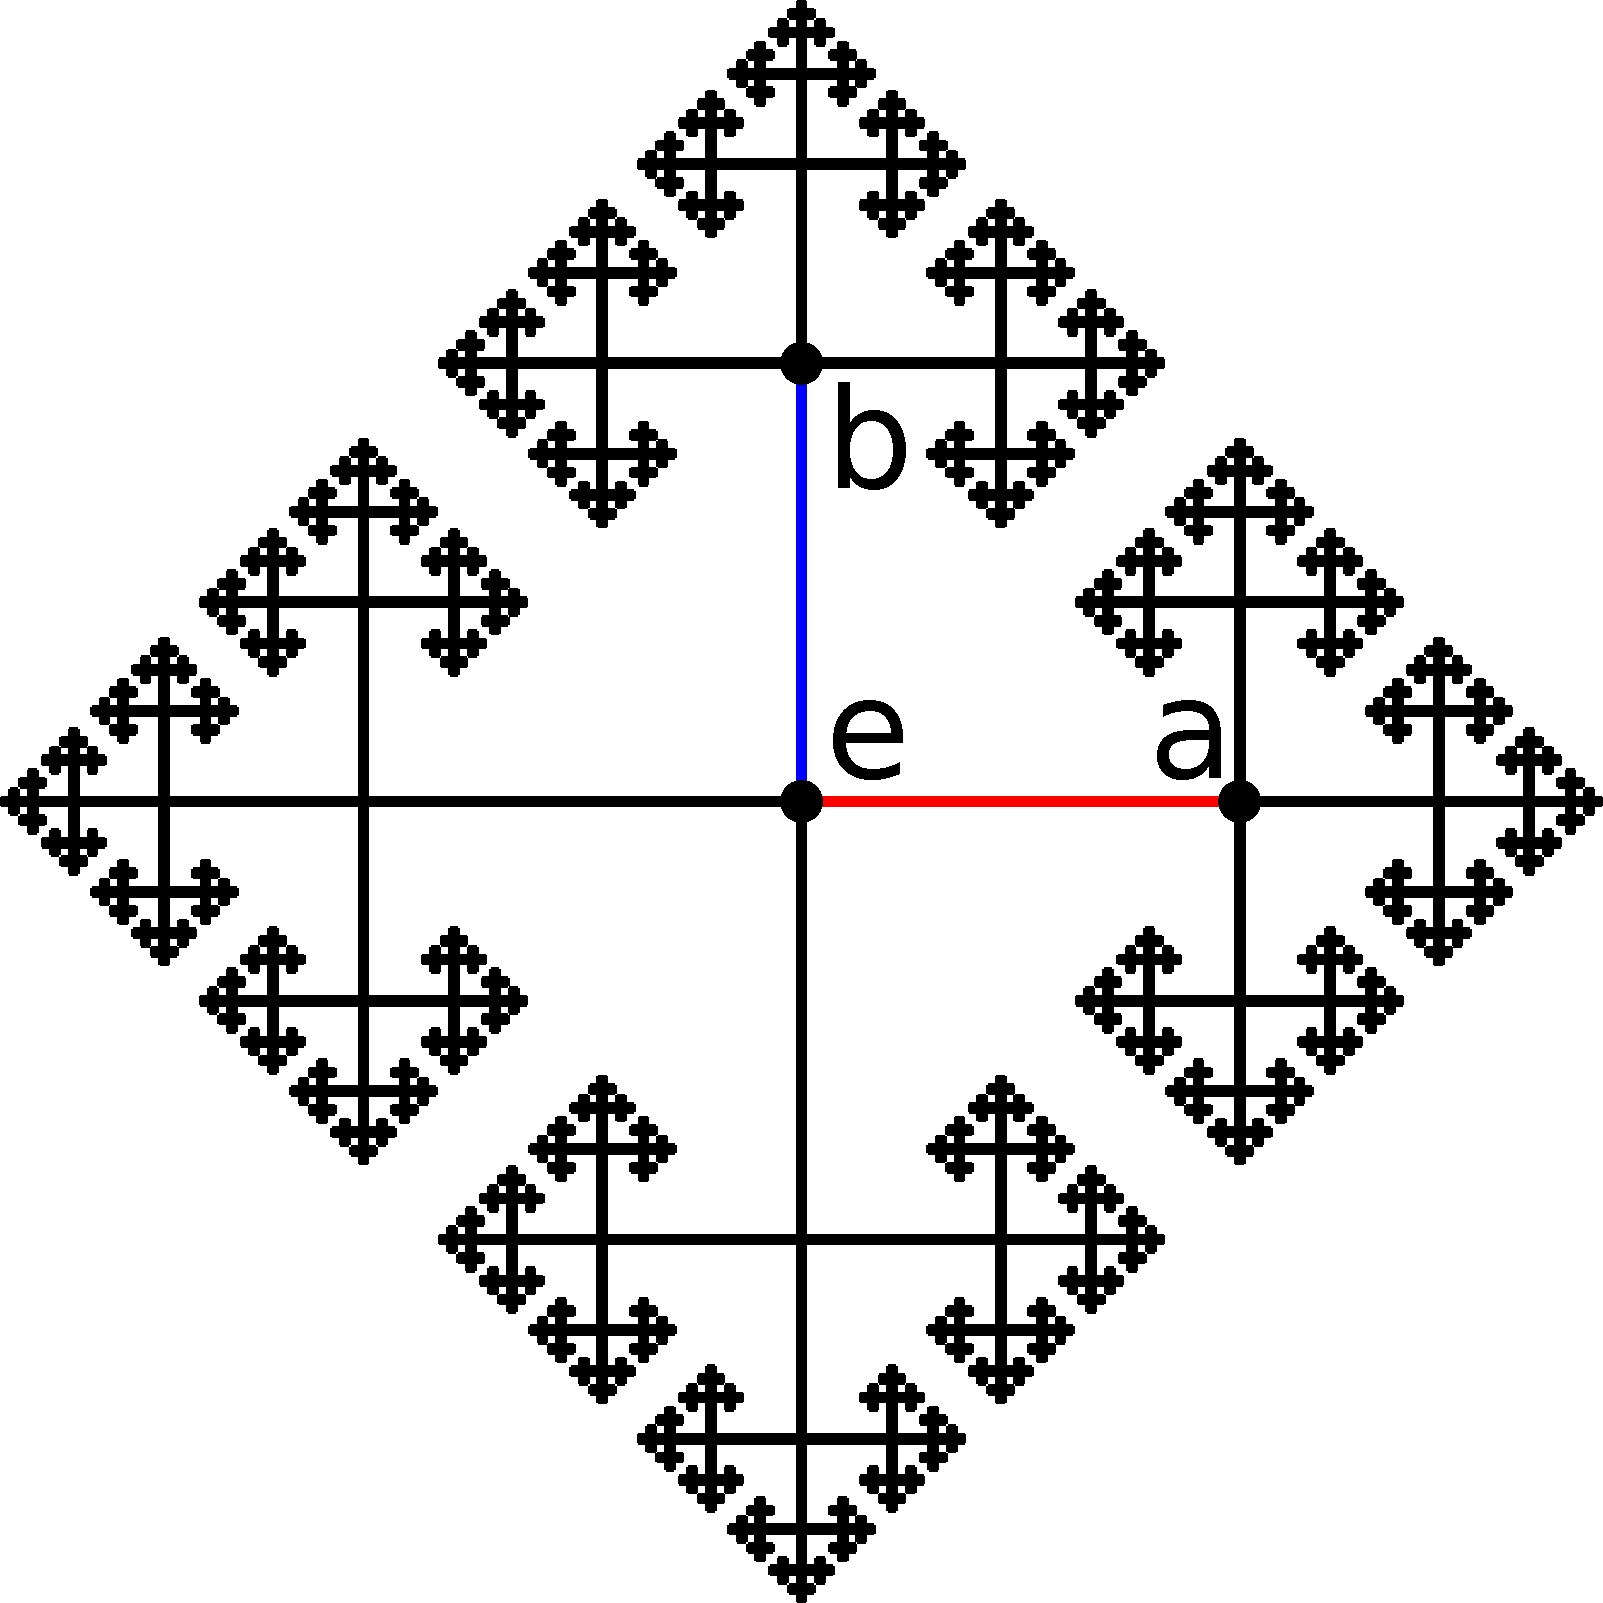
\includegraphics[scale=0.15]{Images/Cayley.pdf}
        \captionof{figure}{This graph is the universal cover of the figure eight, which is $\Gamma=S^1 \vee S^1$. It is also the Cayley graph of the fundamental group of $\Gamma$, i.e.\ the free group with two generators $a$ and $b$, $\pi_1(\Gamma)=F(\{a,b\})\cong\mathbb{Z}\ast\mathbb{Z}$. \label{Fig. Cayley}} 
    \end{minipage}
\end{example}



\begin{xca}
    Show that the universal cover of $M_1\times M_2$ is $\wt M_1\times \wt M_2$.
\end{xca}

\begin{example}
    $\widetilde{T^n}=\mathbb{R}^n$, $\widetilde{\text{SO}_3}=\text{SU}_2=S^3$, $\widetilde{\text{SO}}_{n>2}=\text{Spin}_n$, $\widetilde{\text{U}_n}=\text{SU}_n\times \mathbb{R}$.
\end{example}




\section{Bundles}

\subsection{Fiber Bundles}

We will need only locally trivial fibrations. There are more general notions of Serre and Hurewicz fibrations, and you can find much more about the general theory of fibrations in e.g.\ \cite{Aguilar}. In this text, ``fiber bundle'' will always refer to locally trivial fibrations.

\begin{defn}[Fiber bundle/Locally trivial fibration]\index{Fiber bundle}
A map $\pi\in C^\infty(E,M)$ is a locally trivial fibration, or a \gls{fb}, if it is a smooth submersion and for any $p\in M$ there is an open neighborhood $U_p$ and a diffeomorphism $\chi_p:\pi^{-1}(U_p)\to U_p\times \pi^{-1}(p)$ (recall that $\pi^{-1}(p)$ is a smooth manifold for submersions) such that the following triangle commutes:
\[
\begin{tikzcd}[every matrix/.append style={name=m},   
execute at end picture={\draw [<-] ([xshift=0mm,yshift=-2mm]m-2-2.north) arc[start angle=-90,delta angle=-270,radius=0.25cm];}]
   \pi^{-1}(U_p) \arrow[rr,"\chi_p"]\arrow[ddr,swap,"\restr{\pi}{\pi^{-1}(U_p)}"]& & U_p\times \pi^{-1}(p)\arrow[ddl,"\pi_1"]\\
   & \, & \\
   & U_p & \\
\end{tikzcd}
\]
It is called a \emph{trivial bundle}\index{Trivial bundle} if $U$ can be taken to be all of $M$, i.e.\ the total space decomposes into a product $E\cong M\times \pi^{-1}(p)$. The maps $\chi_p$ are called \emph{local trivializations}.\index{Trivialization}

Finally, a \gls{fb} can be restricted to an open subset $U\subset M$ by defining $\restr{E}{U}$ as $\pi^{-1}(U)\overset{\pi|_{\pi^{-1}(U)}}{\longrightarrow}M$.
\end{defn}

\begin{prop}
For a \gls{fb} $\pi:E\to M$ with $M$ connected, all fibers $\pi^{-1}(m)$ are diffeomorphic to each other. We call a manifold $F$ that they are all diffeomorphic to ``the typical fiber of the fibration''.
\end{prop}
\begin{proof}
A connected manifold is path-connected. By connecting any two points with a path, covering this path by a finite sequence of open sets over which the fibration is trivial, and using the chain of local trivializations, we establish a diffeomorphism between the fibers at the endpoints.
\end{proof}
\begin{example}
\begin{enumerate}
    \item The cylinder $E=S^1\times\mathbb{R}$ is a trivial \emph{line bundle} (or rather the total space of one) over a circle with $\pi$ the projection onto the first factor. It is also a \emph{circle bundle} over the line under the projection onto the second factor.
    \item The M\"obius band is a non-trivial line bundle over the circle under the projection onto the ``equator'' of the band. It is not trivial because it's not homeomorphic to the trivial line bundle, which is the cylinder.
    \item $\mathbb{R}^n\setminus\{0\}$ is a line bundle above the sphere $S^{n-1}$ under $\pi(x)=x/\Vert x\Vert$.
\end{enumerate}
\end{example}


\begin{comment}
    \begin{samepage}
        \PRLsep
        \begin{center}
            {\red Lecture 8 on 18 Jan 2019 ended here}
        \end{center}
    \end{samepage}
\end{comment}


\begin{example}
Covering spaces of $M$ are exactly the \glspl{fb} over $M$ whose fibers are at most countable sets with discrete topology.
\end{example}

The following fundamental theorem gives us a useful sufficient condition for a map to be a locally trivial fibration.

\begin{thm}[Ehresmann fibration theorem]\index{Ehresmann fibration theorem}
If $\pi:E\to M$ is a \emph{proper} surjective submersion, then $\pi$ is a locally trivial fibration.
\end{thm}
\begin{proof}
This is a pretty technically involved theorem, see e.g. \cite{Dundas}. We note only that since the statement is local, it suffices to prove it for $M=\mathbb{R}^n$. Locally (both in $E$ and $M$), all submersions are trivial fibrations. Then we can use flows of vector fields along the fibers of the submersion and a \gls{pou} to glue these trivial pieces together into a locally trivial fibration.
\end{proof}
\begin{cor}
A surjective submersion acting between compact manifolds is a locally trivial fibration.
\end{cor}


\begin{example}[Qubit/Bloch sphere/Hopf fibration]\index{Qubit}\index{Bloch sphere}\index{Hopf fibration}\label{Hopf bundle}
A qubit is a two-level system described by a pair of complex numbers $(\alpha,\beta)\in\mathbb{C}^2$ such that $|\alpha|^2+|\beta|^2=1$. The set of such points is the unit sphere $S^3$ in $\mathbb{C}^2\cong\mathbb{R}^4$. However, points differing only by a phase correspond to the same physical state: $(e^{i\theta}\alpha,e^{i\theta}\beta)\sim(\alpha,\beta)$. It turns out that these equivalence classes are in one-to-one correspondence with points of a two-sphere $S^2$, because the quotient map can be given by
\[\pi(\alpha,\beta)=(\underbrace{|\alpha|^2-|\beta|^2}_{\in [-1,1]},\underbrace{2\alpha\bar\beta}_{\in \mathbb{D}\subset\mathbb{C}})\in S^2\subset\mathbb{R}^3\cong \mathbb{R}\times\mathbb{C}.\]
This is obviously a smooth and surjective map, and since the sphere $S^3$ is compact, it is proper. It is also easy to check that its differential is everywhere surjective, therefore by Ehresmann's theorem $\pi$ is a \gls{fb} with typical fiber $S^1$ (space of phases). This fibration, often written as $S^3\overset{S^1}{\to}S^2$, is called the Hopf fibration, or the Hopf bundle. Since $S^3$ with one point excluded is homeomorphic to $\mathbb{R}^3$, the Hopf fibration is often visualized as a fibration of the 3D space by circles plus one straight line (circle of infinite radius). Any two circles in this fibration happen to be linked with each other, see Fig. \ref{Fig.Hopf}.

$S^2$, which represents the set of physical states of a qubit, is the Bloch sphere. One can show that this fibration is not trivial (the easiest way, perhaps, is to compare the fundamental groups $\pi_1(S^2\times S^1)=\pi_1(S^2)\times\pi_1(S^1)=\mathbb{Z}$ and $\pi_1(S^3)=\{e\}$).

\begin{minipage}[c]{\textwidth}
    \centering
    \captionsetup{type=figure}
    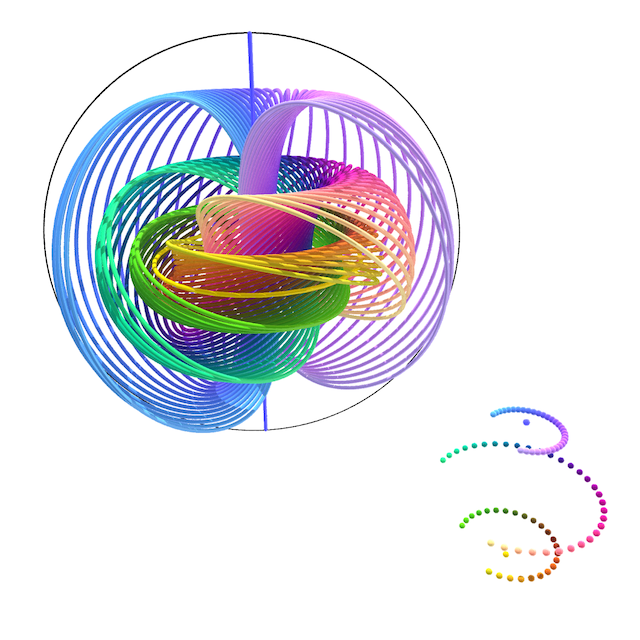
\includegraphics[scale=0.2]{Images/Hopf.png}
    \captionof{figure}{Hopf fibration in stereographic projection, i.e.\ as a fibration of $\mathbb{R}^3$. Each circle is a fiber corresponding to a point on the 2-sphere at the bottom. \cite{hopf}}
    \label{Fig.Hopf}
\end{minipage}
\end{example}

\begin{xca}
Show that in the Hopf bundle, the preimage of any circle in $S^2$ is a two-torus $T^2$ embedded into $S^3$.
\end{xca}


\begin{defn}[Bundle maps]\index{Bundle map}
Let $E\overset{\pi}{\to}M$ and $E'\overset{\pi'}{\to}M'$ be two smooth \glspl{fb}. A bundle morphism (a.k.a.\ \emph{bundle map}) between them is a pair of smooth maps $\wt{h}:E\to E'$ and $h:M\to M'$ such that $\wt{h}$ ``covers'' $h$ in the sense that the following square commutes:
\[\begin{tikzcd}[every matrix/.append style={name=m},   
execute at end picture={\draw [<-] ([xshift=-8mm,yshift=1mm]m-2-2.north) arc[start angle=-90,delta angle=270,radius=0.25cm];}]
   E \arrow[r,"\wt{h}"]\arrow[d,swap,"\pi"]& E'\arrow[d,"\pi'"] \\
   M\arrow[r,swap,"h"]& M'\\
\end{tikzcd}\]
This gives rise to the category $\mathsf{FB}^\infty$ of all smooth \glspl{fb}. A full subcategory is the category $\mathsf{FB}^\infty_M$ of all smooth \glspl{fb} over a given base $M$ (the ``horizontal'' part of every morphism in the latter category is assumed to be $\id_M$).
\end{defn}

\begin{defn}[Lie group]\index{Lie group}
A Lie group $G$ is a smooth manifold with a group structure on it such that the operation $G\times G\to G$ given by $(g,h)\to g^{-1} h$ is smooth (i.e.\ both multiplication and inversion are smooth).
\end{defn}


\begin{defn}[Bundle atlases, cocycles]
Let $E\overset{\pi}{\to}M$ be a smooth \gls{fb} with typical fiber $F$, and let $\{U_\alpha\}_\alpha$ be an open cover of $M$ such that the restrictions $\restr{E}{U_\alpha}$ are trivial. By definition of local triviality, we have some diffeomorphisms $\chi_\alpha: \restr{E}{U_\alpha}\to U_\alpha\times F$, called \emph{local trivializations}. Then:
\begin{itemize}
    \item The collection $\{(U_\alpha,\chi_\alpha)\}$ is called a \emph{\gls{fb} atlas} for $E\overset{\pi}{\to}M$;
    \item For any point $(m,f)\in U_{\alpha\beta}\times F$, the transition maps in this atlas have the form $\chi_\beta\circ\chi_\alpha^{-1} (m,f)=(m, t_{\beta\alpha}(m,f))$, where for every fixed $m\in M$, the map $t_{\beta\alpha}(m,\_):F\to F$ is a diffeomorphism. One can think of $t_{\beta\alpha}$ as a function on $U_{\alpha\beta}$ that takes values in the group $G=\mathrm{Diff}(F)$ of all diffeomorphisms of $F$, so $t_{\beta\alpha}$ becomes a (smooth) map $t_{\beta\alpha}:U_{\alpha\beta}\to G$.\footnote{In a certain precise sense, the group $\mathrm{Diff}(F)$ is an infinite-dimensional Lie group, and $t_{\alpha\beta}$ can be shown to be smooth maps with values in this manifold.} These $G$-valued functions are called \textit{bundle transition functions};
    \item If the transition functions actually take values in a Lie subgroup $G<\mathrm{Diff}(F)$ (i.e.\ a subgroup which is itself a Lie group), then we say that $G$ is the \emph{structure group} of the bundle. If the bundle is isomorphic to a bundle whose structure group is even smaller $H<G$, then we speak of a \emph{bundle reduction} from $G$ to $H$. The ability to reduce to a smaller structure group usually indicates the existence of extra structure on the bundle. E.g.\ a bundle is trivial iff its structure group can be reduced to the trivial group.
    
    \item The group-valued bundle transition functions satisfy two important conditions:
    \[
    \begin{cases}
    t_{\alpha\alpha}\equiv\id_{F}, & \text{(identity condition)}\\
    \restr{t_{\alpha\beta}\circ t_{\beta\gamma}\circ t_{\gamma\alpha}}{U_{\alpha\beta\gamma}}\equiv\id_{F}; & \text{(cocycle condition)}
    \end{cases}
    \]
    Any collection of such $G$-valued functions $\{t_{\alpha\beta}\}$ associated to an open cover of $M$ is called a \emph{cocycle}\index{Cocycle} on $M$ with structure group $G$.
    
    \item \Glspl{fb} can be alternatively defined by specifying the base manifold $M$, the typical fiber $F$, the structure Lie group $G$ acting on the fiber via a Lie (smooth) homomorphism (``representation'') $R:G\to \Diff(F)$ (i.e.\ we will write $g\cdot f=R(g)(f)$ for $g\in G, f\in F$), an open cover $\{U_\alpha\}$ of $M$, and a cocycle  $t_{\beta\alpha}\in C^\infty (U_{\alpha\beta}, G)$. Namely, we can define $E$ as a topological space as the quotient $E\coloneqq \bigslant{(\bigsqcup_\alpha U_\alpha \times F)}{\sim}$, where $(m_1,f_1)\sim(m_2,f_2)$ iff $m_1=m_2=m$ and $f_1=t_{\beta\alpha}(m,f_2)$ for some $\alpha,\beta$, and the projection $\pi$ is defined as the descendent of the projections onto the fist component in each summand.\footnote{In categorical terms, this is literally the cofibered product (pushout) of the sets $U_\alpha \times F$ with pairs of maps $\restr{\chi_\alpha^{-1}}{U_{\alpha\beta}\times F}$ and $\restr{\chi_\beta^{-1}}{U_{\alpha\beta}\times F}$. For instance, if there were only two sets $U_1,U_2$, we would have $E=(U_1\times F)\sqcup_Z (U_2\times F)$, where $Z=U_{12}\times F$ and we have two morphisms $\restr{\chi_i^{-1}}{U_{12}\times F}:Z\to U_i\times F$ that are used in the definition of the pushout.} Then $E$ has a unique smooth structure that makes $\pi$ a smooth submersion (see \cite[Lm. 10.6]{Lee} for the case of vector bundles, which is easily generalized to all \glspl{fb}).\footnote{Essentially we can take an atlas $\{F_\alpha,\psi_\alpha\}$ of $F$ and an atlas $\varphi_\alpha$ of $M$ (\gls{wlog} subordinate to the covering $\{U_\alpha\}$) to construct a smooth atlas $\{(U_\alpha\times F_\beta,\varphi_\alpha\times\psi_\beta)\}$ of $E$.}
    
    \item In local trivializations $\chi_\alpha$, $\chi_\beta'$ on two bundles with the same typical fiber $F$, bundle morphisms that are fiberwise isomorphisms (i.e.\ diffeomorphisms when restricted to one fiber) are represented by $\Diff(F)$-valued functions $\wh{g}_{\alpha\beta}:U_\alpha\to \Diff(F)$: \[\wt{h}\left(\chi_\alpha^{-1}(p,f)\right)=\chi_\beta^{\prime-1}\left(h(p),\wh{g}_{\alpha\beta}(p)\cdot f\right).\]
\end{itemize}
\end{defn}


\begin{defn}[Category ${\sf FB}^\infty(F,G)$]
    Given a Lie group $G$, we introduce the category ${\sf FB}^\infty(F,G)$ of all smooth fiber bundles with typical fiber $F$ (which is assumed to carry an effective $G$-action, i.e.\ an injective smooth homomorphism $G\hookrightarrow\Diff(F)$) that admit a cocycle with structure group $G$. The morphisms is this category are bundle maps that are \emph{fiberwise diffeomorphisms}\footnote{Notice how the set of morphisms is restricted compared to the general category of all fiber bundles.} and are locally represented (w.r.t.\ any two bundle atlases with $G$-valued cocycles) by $G$-valued functions: \[\wt{h}\left(\chi_\alpha^{-1}(p,f)\right)=\chi_\beta^{\prime-1}\left(h(p),\wh{g}_{\alpha\beta}(p)\cdot f\right),\quad \wh{g}_{\beta\alpha}:U_{\alpha\beta}\to G.\]
    Similarly we define the category ${\sf FB}^{\infty}_M(F,G)$ of such fiber bundles over a given base $M$.
\end{defn}

\begin{rem}
    If the structure group $G$ is not $\Diff(F)$ and reflects some additional structure on a bundle, then these are the bundle morphisms that ``respect that structure''. Therefore the smaller the $G$, the more structure the morphisms of this category preserve. We will use this rough idea when introducing vector bundles, orientations, and complex bundles.
\end{rem}

\begin{example}
    Consider the cylinder $E=S^1\times\mathbb{R}$ as a line bundle over the circle. We can trivialize it with all transition functions being the identity. In the category of all line bundles (with structure group $\Diff(\mathbb{R})$) there is a bundle map $E\to E$ that maps $(p,x)\mapsto (p,-x)$. However, in the category of bundles with the trivial structure group $G=\{e\}$ (i.e.\ the category of trivial bundles) this is not an allowed bundle map because it does not act trivially on the fiber. Therefore morphisms in this category must preserve the orientation of the fibers.
\end{example}

The following theorem is one of the most important theorems for the applications of fiber bundle theory, for example in complex-analytic problems of differential equations (where it is known as the Riemann-Hilbert factorization problem).

\begin{thm}\label{bundle isomorphism thm}
Two bundles $E$ and $E'$ over $M$ are isomorphic iff there exists a covering $\{U_\alpha \}$ of $M$, two corresponding cocycles $\{t_{\alpha\beta}\}$ and $\{t_{\alpha\beta}'\}$, and a set of $G$-valued functions $\lambda_\alpha:U_\alpha\to G$ such that $t_{\alpha\beta}'(p)\equiv \lambda_\alpha (p) t_{\alpha\beta}(p) \lambda_\beta^{-1}(p)$ for all $p\in U_{\alpha\beta}$. In particular, a bundle is trivial iff its transition functions can be factorized as $t_{\alpha\beta}=\lambda_\alpha \lambda_\beta^{-1}$.
\end{thm}
\begin{proof}
Exercise. \emph{Hint:} given two bundle atlases over $M$, we can always take all possible pairwise intersections of the sets of the two covers of $M$ to refine the atlases so that they are defined over the same covering of $M$. \gls{wlog}, any isomorphism of bundles over the same base can be assumed be identity on the base itself (e.g. because if the horizontal part of the isomorphism is some diffeo $f:M\to M$, we can replace one of the bundles by the isomorphic pullback bundle along $f$, see Definition \ref{Pullback bundle}). Then any bundle isomophism gives rise to the $\lambda_\alpha$'s, and vice versa, $\lambda_\alpha$'s completely describe the bundle isomorphism. 
\end{proof}


\begin{defn}
	A \gls{fb} is called \emph{flat} if it admits a bundle atlas with constant transition functions. Alternatively, it is a bundle whose structure group can be taken to have a \emph{totally disconnected} topology (one where all connected subsets are one-point sets, e.g. the discrete topology; then the transition functions are forced to be constant by continuity).
\end{defn}

\begin{example}[Line bundles above $S^1$]\label{line bundles over S1}
    We can use the idea of a bundle atlas and Theorem \ref{bundle isomorphism thm} to classify all line bundles above the circle up to isomorphisms. It suffices to pick one covering of the circle, so we will pick a covering by the three circular arcs $U_1=(\epsilon,4\pi/3-\epsilon)$, $U_2=(2\pi/3+\epsilon,2\pi-\epsilon)$, and $U_3=(4\pi/3+\epsilon,8\pi/3-\epsilon)$. The transition functions in a line bundle take values in the group $G$ of diffeomorphisms of $\mathbb{R}$. Each such diffeomorphism is a smooth function $f:\mathbb{R}\to\mathbb{R}$ such that $f'$ is never zero. Now, clearly $G$ consists of two path-connected components, one of diffeomorphisms that preserve the orientation, i.e.\ $f'(x)>0$ for all $x$, and others that reverse it, $f'(x)<0$. We say that these diffeomorphisms have one of two possible \emph{parities}. Let $g_+(x)=\id_{\mathbb{R}}(x)=x$ and $g_-(x)=-x$, so that $g_+$ is the identity element of $\Diff(\mathbb{R})$ and $g_-$ is an orientation-reversing involution.

    There are three transition functions, $t_{12}$, $t_{23}$, and $t_{31}$. Any three $G$-valued functions $\lambda_1,\lambda_2,\lambda_3$ provide an isomorphic line bundle. Choose $\lambda_1\equiv g_+$. Furthermore, $t_{12}:U_{12}\to G$ can be extended to a continuous function $\lambda_2: U_2\to G$, $\restr{\lambda_2}{U_{12}}=t_{12}$. Then $t_{12}'=\lambda_1 t_{12}\lambda_2^{-1}\equiv g_+$. By continuity, all values of $\lambda_2$ have the same parity.  Now, we let $\lambda_3$ be a continuous extension to $U_3$ of the function $\lambda_2 t_{23}:U_{23}\to G$. Then $t_{23}'=\lambda_2 t_{23} \lambda_3^{-1}\equiv g_+$. Finally, $t_{31}'=\lambda_3 t_{31} \lambda_1=\lambda_3 t_{31}$.  The parity of the values of $t_{31}'$ by construction is the product of the parities of $t_{12}$, $t_{23}$, and $t_{31}$.

    The values of $\lambda_3$ are already uniquely fixed up to the point $2\pi-\epsilon=-\epsilon$. Due to the path-connectedness of the two components of $G$, $\lambda_3$ can be deformed on $U_3\setminus U_{23}=(-\epsilon,2\pi/3-\epsilon)$ so that it remains smooth and $\restr{\lambda_3}{(\epsilon,2\pi/3-\epsilon)}=g_\pm t_{31}^{-1}$, which leads to $t_{31}'\equiv g_\pm$.

    This means that any line bundle above $S^1$ is isomorphic to one of two bundles, whose transition functions are either all identities, or one of them is a reflection $x\mapsto -x$.  In other words, any line bundle over $S^1$ can be reduced to the structure group $O(1)=\mathbb{Z}_2$. The former bundle is trivial, and the latter bundle is homeomorphic to the M\"obius band. There are only two isomorphism classes of line bundles above $S^1$.
\end{example}

\begin{xca}\label{Rk-bundles above circle}
    Show that there are only two isomorphism classes of \glspl{fb} with fiber $\mathbb{R}^k$  above $S^1$ for any $k$.
\end{xca}


\begin{example}[Covering spaces and flat bundles with flat connections]
	Covering spaces are just \glspl{fb} with discrete fibers, therefore their structure group $G$ is the permutation group of the points of the typical fiber. The classification theorem for covering spaces stated that all bundles over $M$ with the discrete fiber $F$ are classified by all possible homomorphisms $\pi_1(M)\to G$ (up to global conjugation by an element of $G$ corresponding to a shuffling of the points of $F$).
	
	Continuing Remark \ref{covering spaces and connections}, we see that the monodromy, or holonomy, is also nothing but a representation of $\pi_1(M)$ on the fiber. Therefore bundles with discrete fibers are completely classified by the monodromy/holonomy of the connection on them. Can we generalize these ideas to a larger class of bundles?
	
	First of all, by a simple extension of the argument in Example \ref{line bundles over S1}, we see  that all bundles with fiber $F$ and structure group $G$ above $S^1$ are classified by homomorphisms $\Hom(\pi_1(M),\pi_0(G))/\sim$, where $\pi_0(G)=G/G_0$ and $G_0$ is the connected component of the identity in $G$ (which is a normal subgroup), so that $\pi_0(G)$ is the group whose elements are the connected components of $G$. The equivalence relation is the global conjugation of all values of the given homomorphism by an arbitrary element of the target group (corresponds to a diffeomorphism on $F$, which of course doesn't change the bundle). For instance, for $F=\mathbb{R}$ and $G=\Diff(\mathbb{R})$, we found that $\pi_0(G)=\mathbb{Z}_2$. The statement also agrees with the classification theorem for covering spaces.
	
	Recall that a connection is just a prescription for lifting curves from the base into the total space. The lifted curves are called \emph{horizontal}, and the lifting procedure is also known as \emph{parallel transport} (of the starting point in the bundle along the path in the base). If the curve in the base is a loop $\gamma$ such that $\gamma(0)=\gamma(1)=p\in M$, then its lifts with all possible starting points $\wt{\gamma}(0)=e_0\in E_p$ determine the holonomy $e_0\mapsto e_1=\wt{\gamma}(1)=h(\gamma)(e_0)$, where we introduced the map $h:\gamma\mapsto h(\gamma)\in G$. Defined this way, $h(\gamma)$ is an element of the structure group $G$, and moreover $h$ is a homomorphism from the group $L_p(M)$ of all loops based at $p$ to $G$. The image of this homomorphism is a subgroup $\mathrm{Hol}_p<G$ called the \emph{holonomy group} of the bundle based at $p$. If $h$ is restricted only to contractible loops, then the corresponding group is called $\widetilde{\mathrm{Hol}}_p<\mathrm{Hol}_p<G$, the \emph{local holonomy} group at $p$. 
	
	If $\widetilde{\mathrm{Hol}}_p=\{\id\}$ for all $p$, the connection is called \emph{flat}. This is equivalent to the property that the holonomy depends only on the homotopy class of the base loop. In particular, a small simply connected neighborhood $U\subset M$ of $p\in M$ can be uniquely lifted to a local section of $E$ passing through $e_0\in E_p$, which is of course diffeomorphic to $U$. That is, $E$ can be locally fibrated by horizontal sections, each diffeomorphic to $U$. 
	
	Flatness of a connection is sometimes called \emph{integrability}\index{Integrability}, and is exactly what people mean when they speak of integrable systems in physics: the phase space of an integrable system can be fibrated by hypersurfaces that are locally spanned by physical trajectories.
	
	Finally, we notice that the definition of flat \glspl{fb} given above implies the existence of a flat connection. Namely, a loop $\gamma$ in $M$ that passes through charts $U_1,U_2,\ldots,U_n=U_1$ with the starting point $(p,f)\in U_1\times F$ can be lifted as $(\gamma(t),f)$ on $U_1$, $(\gamma(t),\tau_{21}f)$ on $U_2$, $(\gamma(t),\tau_{32}\tau_{21}f)$ on $U_3$, and so on (here $\tau_{ij}\in G$ represent the constant transition functions). These actually stitch together into a continuous path under the identifications in the bundle. Similarly one can lift non-closed curves, which completes the definition of the connection.
	
	Exercise: check that the local holonomy of the connection just described is independent of the choice of a bundle atlas (even though the connection itself does depend on the atlas) and trivial , i.e.\ the connection is indeed flat.
	
	The non-local part of the holonomy is described by ordered products of transition functions $\prod \tau_{ij}$ along non-contractible loops. Since these are homotopy-invariant, we have a homomorphism $\pi_1(M)\to G$ that completely describes the holonomy of the flat connection. A global conjugation $g\mapsto g_0 g g_0^{-1}$ on the group doesn't affect the connection (it is essentially equivalent to shifting the base point in the definition of $\pi_1(M)$), therefore all flat connections on bundles with structure group $G$ above $M$ are classified by $\Hom(\pi_1(M),G)/\sim$, where $\sim$ is the conjugation equivalence. Moreover, one can show that every homomorphism of this kind corresponds to a bundle with a connection. This is the generalization of the classification theorem for covering spaces.
	
	Note that a flat bundle with structure group $G$ and a flat connection is the same as a fiber bundle whose structure group is $G$ with the discrete topology (because in the latter situation the transition functions as well as all deformation parameters $\lambda_\alpha$ are forced to be constant functions, the flat connection is unique and given by the construction above). All this leads us to conclude that flat bundles with a flat connection, or bundles with totally disconnected structure groups, are the natural generalization of covering spaces.
	
	We have shown that bundles over $M$ with a totally disconnected structure group $G$ are precisely classified by the conjugacy classes of homomorphisms $\Hom(\pi_1(M),G)$. The conjugacy class of such homomorphisms corresponding to a bundle $E\overset{\pi}{\to}M$ is called the \emph{characteristic class}\index{Characteristic class} of the bundle. Therefore, for totally disconnected structure groups, a single characteristic class determines the isomorphism class of the bundle.
	
	The main goal for Parts \ref{Part II} and \ref{Part III} of these lectures will be to develop the machinery necessary for the full classification of \glspl{fb} with arbitrary topological structure groups, in particular by extending the theory of characteristic classes. The characteristic class we have just constructed (acting on one-dimensional cycles, i.e.\ closed loops) is only the first one in an infinite list of cohomology classes corresponding to a given bundle.
	
\end{example}

\begin{comment}
    \begin{samepage}
        \PRLsep
        \begin{center}
            {\red Lecture 9 on 25 Jan 2019 ended here}
        \end{center}
    \end{samepage}
\end{comment}

\subsection{Homotopy Lifting Property}
    We've seen that bundles are, in categorical terms, pushouts (i.e.\ quotients of disjoint unions) of a family of trivial bundles along the trivialization maps. The categorical notion of pullback introduced in Definition \ref{pullbacks} is also very useful in the theory of \glspl{fb}.

\begin{defn}[Pullback bundle]\index{Pullback bundle}\label{Pullback bundle}
    Let $E\overset{\pi}{\to}M$ be a smooth \gls{fb} and $N\overset{f}{\to}M$ a smooth map. We define the \emph{pullback bundle} $f^\ast E$ in three ways:
    \begin{itemize}
        \item In categorical terms, it is literally the pullback $E\times_M N$ that uses the maps $E\overset{\pi}{\to}M$ and $N\overset{f}{\to}M$ in its Cartesian square. This object indeed exists because it can be explicitly constructed using either of the next two alternative definitions. The pullback naturally comes with two canonical projections $f^\ast E\overset{\wt{f}}{\to}E$ and $f^\ast E\overset{\pi'}{\to}N$.
        \item $f^\ast E=\{(p,n)\in E\times N\mid f(n)=\pi(p)\}\subset E\times N$ with the subspace topology induced from $E\times N$. Obviously we have two canonical projections onto the two components of the product, $f^\ast E\overset{\wt{f}}{\to}E$ and $f^\ast E\overset{\pi'}{\to}N$. The latter one is the new bundle projection. We show below that there is a unique smooth structure on $f^\ast E$ that makes $\pi'$ into a smooth submersion.
        \item If the typical fiber of $E$ is $F$ and we know a set of transition functions $t_{\alpha\beta}:U_{\alpha\beta}\to G$ defining $E$, then $f^\ast E$ can be defined as the bundle with base $N$, same fiber $F$, and transition functions $f^\ast t_{\alpha\beta}:f^{-1}(U_{\alpha\beta})\to G$, where $f^\ast t\equiv t\circ f$ is the definition of the \emph{pullback of a function} $t$ on $M$ via $f$.
    \end{itemize} 
    \[\begin{tikzcd}[every matrix/.append style={name=m},   
    execute at end picture={\draw [<-] ([xshift=-8mm,yshift=1mm]m-2-2.north) arc[start angle=-90,delta angle=270,radius=0.25cm];}]
   f^\ast E \arrow[r,"\wt{f}"]\arrow[d,swap,"\pi'"]& E\arrow[d,"\pi"] \\
   N\arrow[r,swap,"f"]& M\\
    \end{tikzcd}\]
\end{defn}

\begin{prop}
\begin{enumerate}
    \item $f^\ast E$ defined via any of the last two definitions has a unique smooth structure that turns the bundle projection into a smooth submersion.
    \item All three definitions are isomorphic as smooth bundles.
    \item $f^\ast E$, defined as in the second definition, is in fact an embedded submanifold of $E\times N$.
\end{enumerate} 
\end{prop}
\begin{proof}
    We don't give a full proof here. The fact that $f^\ast E$ is a smooth \gls{fb} is manifest in the third definition of the pullback bundle.
\end{proof}

\begin{xca}
\begin{enumerate}
    \item Show that if $E$ is trivial, then $f^\ast E$ is trivial for any $f$. In other words, pullbacks of bundles are always ``at least as trivial'' as the original bundles.
    \item Show that if $(\wt{f},f)$ is a bundle map from $E$ to $E'$ that is also a fiberwise diffeomorphism, then $E\cong f^\ast E'$.
\end{enumerate}
\end{xca}

\begin{defn}[Restriction of a bundle]
    If $S< M$ via the immersion $i:S\to M$ and $E\overset{\pi}{\to}M$ is a smooth \gls{fb}, then we can define the restricted bundle $\restr{E}{S}\coloneqq i^\ast E$. It is a smooth \gls{fb} by the last proposition.
\end{defn}


\begin{thm}[Bundles over $M\times I$]\label{bundles over MxI}
    Every \gls{fb} $E$ over $M\times I$, where $I=[0,1]$, is isomorphic to $E_0\times I$ where $E_0=\restr{E}{M\times\{0\}}$. The isomorphism can be chosen so that its restriction to $E_0$ is the inclusion $E_0\hookrightarrow E\times I$ as $p_0\mapsto (p_0,0)$.
\end{thm}
\begin{proof}
    First we show that $E$ can be trivialized over a locally finite open cover of the form $\{U_i\times I\}_i$.

    By local triviality, for a fixed $x\in M$ and every $t\in I$, there is an open neighborhood $V_t\subset M$ of $x$ and an open interval $t\in I_t\subset I$ such that $E$ is trivial over $V_t\times I_t$. Therefore we can construct a countable, locally finite open cover of $M\times I$ with sets of this kind. By compactness, there is a finite set $0<t_1<\cdots<t_k<1$ such that $\bigcup_i I_{t_i}=I$. Let $V_i=V_{t_i}$, $I_i=I_{t_i}$, and define 
    \[
        U_i=\bigcap_{j=1}^i V_j,\quad J_i=\bigcup_{j=1}^i I_j.
    \]
    Obviously $E$ is trivial over $U_1\times J_1$. Let $\chi_1$ be a trivialization of $E$ over $U_1\times J_1$ and $\wt{\chi}_2$ -- one over $V_2\times I_2$. Then $(U_1\times J_1)\cap (V_2\times I_2)=U_2\times (J_1\cap I_2)$. Assuming that $I_2$ intersects $J_1$ non-trivially and one is not contained in the other (otherwise $I_2$ can be dropped from the covering of $I$), consider the transition function $\tau:U_2\times(J_1\cap I_2)\to G$ defined by $\chi_1(p)=\left(\id\times    \tau(\pi(p))\right)\cdot \wt{\chi}_2(p)$. Choose $c\in J_1\cap I_2$ and a continuous function $f:I_2\to J_1\cap I_2$ such that $f(t)=t$ for $t\geq c$ to define 
    \[
        \wt{\tau}:U_2\times I_2\to G,\quad \wt{\tau}(x,t)=\tau(x,f(t)).
    \]
    Clearly $\tau$ and $\wt{\tau}$ coincide on $U_2\times([0,c]\cap I_2)$. Hence the new mapping
    \[
    \chi_2(p)=\begin{cases}
    \chi_1(p), & \pi(p)\in U_2\times[0,c],\\
    (\id\times\wt{\tau}(\pi(p)))\cdot \wt{\chi}_2(p), & \pi(p)\in U_2\times I_2
    \end{cases}
    \]
    defines a trivialization of $E$ over $U_2\times I_2$. By induction, we find that $E$ is trivial over every every $U_i\times I$. 

    Since this construction applies to every $x\in M$, we can extract a locally finite open cover of the entire $M$ of the form $\{U_i\times I\}_i$ such that $E$ is trivial over every set in the covering. Let $\chi_i$ be the corresponding local trivializations and $\wh{\chi}_i$ the induced local trivializations of $\restr{E_0}{U_i}\times I$.

    For $V_1=U_1$, there is an isomorphism $\Phi_1:\restr{E}{V_1\times I}\to\restr{E_0}{V_1}\times I$. We can construct a chain of open sets $V_1\subset V_2\subset\cdots$ that eventually covers all $M$ and $U_i\subset V_i$, and by induction extend the isomorphism to $\Phi_i:\restr{E}{V_i\times I}\to\restr{E_0}{V_i}\times I$. Via the local trivializations $\chi_i$ and $\wh{\chi}_i$, bundle isomorphisms are represented by $G$-valued functions $g_i:U_{i}\times I\to G$ with $g_i(x,0)=e\in G$. Let $g_1:(V_1\cap U_2)\times I\to G$ be the representative of $\Phi_1$ in $\chi_2$ and $\wh{\chi}_2$. Then $g_1$ can be smoothly extended to $V_2\times I$ so that it equals $e$ on $(U_2\setminus V_1)\times I$. This represents the isomorphism $\Phi_2$ that agrees with $\Phi_1$ on the common domain. Repeating this procedure on $U_3$ and so on, we construct a global isomorphism of the bundles in question.

    See \cite[Thm. 3.3.1]{RS2} for details.
\end{proof}

\begin{cor}
    Continuous deformations (homotopies) of transition functions within the class of cocycles don't change the isomorphism class of a fiber bundle.
\end{cor}

Therefore, in the most general and abstract sense, the ``full'' characteristic class\index{Characteristic class} of a fiber bundle (which uniquely classifies the bundle) is the homotopy equivalence class of cocycles for it.

Now we are ready to prove the generalization of the path lifting property of covering spaces.

\begin{thm}[Homotopy Lifting Property/Covering Homotopy Theorem]\label{HLP}
    Let $E\overset{\pi}{\to}M$ and $E'\overset{\pi'}{\to}M'$ be smooth \glspl{fb} with the same typical fiber $F$. If $(\wt{H}_0,H_0)$ is a bundle map from $E$ to $E'$ and $H:M\times I\to M'$ is a homotopy of $H_0$, i.e.\ $H_0=\restr{H}{M\times\{0\}}$, then there exists a bundle map $\wt{H}$ that covers $H$:
    \[\begin{tikzcd}[every matrix/.append style={name=m}, execute at end picture={\draw [<-] ([xshift=-9mm,yshift=1mm]m-2-2.north) arc[start angle=-90,delta angle=270,radius=0.2cm];}]
    E\times I \arrow[r,"\wt{H}"]\arrow[d,swap,"\pi\times\id"]& E'\arrow[d,"\pi'"] \\
    M\times I\arrow[r,swap,"H"]& M'\\
    \end{tikzcd}\]
\end{thm}
\begin{proof}
    Consider the map
    \[
    \lambda:E\to H_0^\ast E'\subset M\times E',\; \lambda(p)=(\pi(p),\wt{H}_0(p)).
    \]
    This is a bundle isomorphism of two bundles over $M$. Moreover, by Theorem \ref{bundles over MxI}, there exists a bundle isomorphism 
    \[
    \Phi:H^\ast E'\to \wt{H}_0^\ast E'\times I
    \]
    of bundles over $M\times I$ satisfying $\Phi\left((x,0),f\right)=\left((x,f),0\right)$. Together with the natural bundle morphism $\proj_2:H^\ast E'\to E'$, the isomorphisms $\lambda $ and $\Phi$ combine to a morphism
    \[
    \wt{H}:E\times I\overset{\lambda\times\id_I}{\longrightarrow}H_0^\ast E' \times I\overset{\Phi^{-1}}{\to}H^\ast E'\overset{\proj_2}{\to}E'
    \]
    that covers $H$. Since 
    \[
    \wt{H}(p,0)=\proj_2\circ\Phi^{-1}\left(\left(\pi(p),\wt{H}_0(p)\right),0\right)=\proj_2\circ \left(\left(\pi(p),0\right),\wt{H}_0(p)\right)=\wt{H}_0(p),
    \]
    $\wt{H}$ is indeed an extension of $\wt{H}_0$.
\end{proof}


\begin{rem}
The Path Lifting Property of covering spaces is a special case of the Homotopy Lifting Property when $M$ consists of one point, but with an extra uniqueness result that doesn't hold for general \glspl{fb}. In topology, fiber bundles (called Hurewicz fibrations, or the even more general Serre fibrations) are in fact defined through the Homotopy Lifting Property.
\end{rem}


\begin{cor}\label{HLP cor}
\begin{enumerate}
    \item If $E'\overset{\pi'}{\to}M'$ is a \gls{fb} and $f,g:M\to M'$ are two smooth maps that are homotopic to each other, then the pullback bundles $f^\ast E'$ and $g^\ast E'$ are isomorphic.
    \item All \glspl{fb} over contractible base spaces are trivial.
    \item Isomorphism classes of \glspl{fb} with fiber $F$ and structure group $G$ over the sphere $S^n$, $n\geq 1$, are in one-to-one correspondence with the homotopy classes of maps from $S^{n-1}$ to the connected component of the identity $G_0$, up to conjugation by the discrete group of connected components of $G$:
    \[
    \mathsf{Sk}\left(\mathsf{FB}_{S^n}(F,G)\right)\cong [S^{n-1},G_0]/\pi_0(G)= \pi_{n-1}(G)/\pi_0(G),\label{FB(G) and homotopy(G)}
    \]
    (here the group $\pi_0(G)$ acts on the set $\pi_{n-1}(G)$ by conjugation of the values, which is a well-defined action within homotopy classes). In particular, when $G$ is connected, this set of isoclasses of fiber bundles forms a group isomorphic to $\pi_{n-1}(G)$.
\end{enumerate}
\end{cor}

\begin{proof}
\begin{enumerate}
    \item Let $H:M\times I\to M'$ be a homotopy from $f$ to $g$ and consider the bundle $P=H^\ast E'$ over $M\times I$. Let $P_t=\restr{P}{X\times\{t\}}$ viewed as a bundle over $M$. Then $P_0=f^\ast E'$ and $P_1=g^\ast E'$. By the above Theorem, $P$ is isomorphic to $P_0\times I$. By restricting the isomorphism to the subbundle $P_1\subset P$, we get an isomorphism from $P_1$ to $P_0$.
    \item Contractible spaces by definition are homotopy equivalent to a point, and all bundles over a point are trivial.
    \item 
    We have already proven this for $n=1$ in Example \ref{line bundles over S1}. For $n\geq 2$, $S^n$ can be covered by two hemispheres $U_\pm$ that overlap along a neighborhood $U_0$ of the equator. The equator $C$ is diffeomorphic to $S^{n-1}$ and $U_0$ can be chosen so that $U_0\cong S^{n-1}\times (-1,1)$. Then the only transition function in any given bundle $E\overset{\pi}{\to}S^n$ is $\tau:U_0\to G$. It can be chosen so that is maps a given point $x_0\in C$ to $e\in G$. Its restriction to the equator provides a map called a \emph{clutching function}\index{Clutching function} $\theta=\restr{\tau}{C}:S^{n-1}\to G_0$ whose homotopy class will be the one put into correspondence to the bundle. 
     
    To check that this mapping is consistent, we need to show that isomorphic bundles have homotopic clutching functions, up to conjugation by an element of $\pi_0(G)$. Let the two transition functions be $\tau_1$ and $\tau_2$ and consider an isomorphism given by $\tau_2=\lambda_+ \tau_1 \lambda_-^{-1}$, where $\lambda_\pm$ are two $G$-valued functions on $U_\pm$, respectively. Since $\tau_{1,2}(x_0)=e$, we can first consider the case when $\lambda_\pm(x_0)=e$ and therefore $\lambda_\pm$ take values in the connected component of the identity $G_0\subset G$. Then we can deform $\lambda_\pm$ by a homotopy so that $\lambda_+(P_+)=\lambda_-(P_-)=e\in G$, where $P_\pm$ are the respective poles of the sphere. Since $U_\pm $ are both diffeomorphic to a ball $B^n\in\mathbb{R}^n$, we can use the Cartesian coordinate $x$ on the ball to introduce the homotopy $\lambda_+(tx)\tau_1(x) \lambda_-^{-1}(tx)$ from $\tau_1$ to $\tau_2$. 
    
    Another choice for $\lambda_\pm$ is when $\lambda_+(x_0)=\lambda_-(x_0)=g_0$ with $g_0$ in another connected component of $G$ than the identity. Then the same argument leads to clutching functions that are, up to a homotopy, conjugates of each other by $g_0$. Different choices of $g_0$ within its connected component only change the clutching functions by a homotopy, just like above, because each connected component of $G$ is path-connected.
    
    Finally, the map constructed is clearly surjective because every function $S^{n-1}\to G_0$ can be used to construct a fiber bundle. It is also injective because any two homotopic clutching functions $\theta_1\sim\theta_2:S^{n-1}\to G$ can only be restrictions of two homotopic transition functions $\tau_1\sim\tau_2:S^{n-1}\times(-1,1)\to G$ (all up to conjugation by $\pi_0(G)$). This is because every such $\tau(x,t)$ is homotopic to one that is independent of $t$ (and this is because every function on $(-1,1)$ is homotopic to a constant one).
\end{enumerate}
\end{proof}

We refer the reader to \cite{HatcherVB} for more details on these classifications of bundles.

\begin{example}
Now we can easily solve Exercise \ref{Rk-bundles above circle}. Consider only vector bundles of rank $k$ above $S^1$. The structure group is $G=\GL_k(\mathbb{R})$. This group has two connected components distinguished by the sign of the determinant. Therefore $\pi_0(G)=\mathbb{Z}_2$ and there are only two isoclasses of bundles. Equivalently we can classify bundles with a two-point fiber $\mathbb{Z}_2$ above $S^1$. We have $G=\Diff(\mathbb{Z}_2)=\mathbb{Z}_2$ and
\[
    \mathsf{FB}_{S^1}(\mathbb{Z}_2)\cong \pi_{0}\left(\mathbb{Z}_2\right)=\mathbb{Z}_2.
\]
\end{example}
\begin{example}
Let us classify all $\mathbb{R}^2$-bundles over $S^2$. We have by Corollary \ref{HLP cor} that 
\[
    \mathsf{FB}_{S^2}(\mathbb{R}^2)\cong \pi_{1}\left(\GL_2(\mathbb{R})\right)/\pi_0\left(\GL_2(\mathbb{R})\right)=\mathbb{Z}/\mathbb{Z}_2\cong \mathbb{N}_0
\]
(because the conjugation of a rotation of the plane by the orientation-reversing reflection gives the opposite rotation). Similarly we can classify circle bundles above the 2-sphere. The structure group of circle bundles is $\Diff(S^1)$, which is homotopy equivalent to $\rm{O}(2)\cong S^1\sqcup S^1$. Therefore
\[
    \mathsf{FB}_{S^2}\left(S^1,\rm{O}(2)\right)\cong \pi_{1}\left(\rm{O}(2)\right)/\pi_0\left(\rm{O}(2)\right)=\mathbb{Z}/\mathbb{Z}_2\cong\mathbb{N}_0.
\]
If we were to restrict the structure group to orientation-preserving diffeomorphisms of the circle, we would need to replace $\mathrm{O}(2)$ by $\mathrm{SO}(2)=\mathrm{U}(1)$, so 
\[
    \mathsf{FB}_{S^2}(S^1,\mathrm{U}(1))\cong \pi_{1}\left(S^1\right)=\mathbb{Z}.
\]
The integer number that classifies these (oriented) plane or circle bundles over the 2-sphere is called the \emph{Chern number}\index{Chern number} and represents yet another characteristic class of bundles.
\end{example}

\begin{example}[Hopf bundle revisited]
    If we cover $S^2$ by two disks $D_\pm$ overlapping along the equator, the Hopf fibration $E\overset\pi\to S^2$ (Example \ref{Hopf bundle}) restricted to each of them is trivial and diffeomorphic to a solid torus in $\mathbb{R}^3$. Therefore the 3-sphere $S^3$ can be broken up into two disjoint (aside from their boundary) solid tori that are glued to each other along the 2-torus that is their common boundary.The twists of the boundary performed in this process classify the resulting circle bundles over the 2-sphere, so here we will try to understand the case of the Hopf bundle. In terms of the coordinates on the bundle used in Example \ref{Hopf bundle}, we have 
    \[\restr{E}{D_+}=\{|\alpha|\geq|\beta|\},\quad \restr{E}{D_-}=\{|\alpha|\leq|\beta|\}.\]
    In addition, over the equator $C$ we have 
    \[\restr{E}{C}=\{|\alpha|^2=|\beta|^2=\frac12\},\]
    so the restriction of the Hopf bundle to the equator is a 2-torus with two angular coordinates $\varphi,\psi$, where $\varphi$ is the standard azimuthal coordinate on the sphere and $\psi$ is the coordinate in the fiber:
    \[\restr{E}{C}=\left\{(\alpha,\beta)=\frac{1}{\sqrt{2}}\left(e^{i\varphi/2+i\psi},e^{-i\varphi/2+i\psi}\right)\right\}.\]
    Identifying $D_\pm$ with the unit disk $\mathbb{D}\subset\mathbb{C}$, we construct the bundle atlas
    \begin{align}
        \chi_+(\alpha,\beta)=\left(\frac{\wb\beta}{\wb\alpha},\frac{\alpha}{|\alpha|}\right)\in\mathbb{D}\times S^1,\quad 0\leq|\beta|\leq |\alpha|\;,0<|\alpha|\leq 1,\\
        \chi_-(\alpha,\beta)=\left(\frac{\alpha}{\beta},\frac{\beta}{|\beta|}\right)\in\mathbb{D}\times S^1,\quad 0\leq|\alpha|\leq|\beta|,\; 0<|\beta|\leq 1.
    \end{align}
    The complex conjugation in $\chi_+$ is there only to make sure that a point above the equator is mapped to the same point on $\partial\mathbb{D}$ by both trivializations. These trivializations are indeed diffeomorphisms because their inverses are
    \begin{align}
        \chi_+^{-1}(z,e^{i\psi})=\left(\frac{e^{i\psi}}{{\sqrt{1+|z|^2}}},\frac{\wb{z}e^{i\psi}}{{\sqrt{1+|z|^2}}}\right),\quad (z,e^{i\psi})\in \mathbb{D}\times S^1,\\
        \chi_-^{-1}(z,e^{i\psi})=\left(\frac{ze^{i\psi}}{{\sqrt{1+|z|^2}}},\frac{e^{i\psi}}{{\sqrt{1+|z|^2}}}\right),\quad (z,e^{i\psi})\in \mathbb{D}\times S^1.
    \end{align}
    It is clear that the clutching function on the equator $z=e^{i\varphi}$ is 
    \[\tau_{-+}(z)\cdot e^{i\psi}=\pr_2\circ \chi_-\circ \chi_+^{-1}(z,e^{i\psi})=z^{-1}\cdot e^{i\psi},\]
    that is, $\tau_{-+}(e^{i\varphi})=e^{-i\varphi}$ (representing the diffeomorphism that acts on the unit circle by multiplication by $e^{-i\varphi}$). Therefore, following a standard sign convention, the Chern number of this bundle equals $-1$.\footnote{The sign of the Chern number is usually fixed by the holomorphic structure of the corresponding bundle (which includes a specific orientation on the fibers). The Hopf bundle is the circle bundle of the complex line bundle $\mathcal{O}(-1)$ defined over the Riemann sphere $S^2=\mathbb{C}P^1$ as the complex line bundle with the transition function $t_{0\infty}(z)=z^{-1}$, and the Chern number of any holomorphic line bundle equals its degree, which in this case is $-1$.}
\end{example}

\begin{xca}
    Show that the Hopf bundle doesn't have any global sections, i.e.\ smooth maps $\sigma:S^2\to E$ such that $\pi\circ\sigma=\id_{S^2}$.
\end{xca}

The last part of the above Corollary shows the importance of the computation of homotopy groups of at least the classical Lie groups. 
\[\boxed{\begin{array}{c}
    \text{Our ultimate goal for Part \ref{Part III} of the lectures will be}\\ 
    \text{to extend (\ref{FB(G) and homotopy(G)}) to arbitrary base manifolds using the theory of characteristic classes.}
\end{array}}
\] 

\begin{comment}
    \begin{samepage}
        \PRLsep
        \begin{center}
            {\red Lecture 10 on 1 Feb 2019 ended here}
        \end{center}
    \end{samepage}
\end{comment}





\subsection{Vector Bundles}

Vector bundles are nothing but \glspl{fb} whose fibers carry vector space structures such that these structures, in some sense, vary smoothly with the base point. We make this precise by putting a natural restriction on the transition functions.

\begin{defn}[Vector bundle]\index{Vector bundle}
A \gls{vb} is a \gls{fb} $E\overset{\pi}{\to}M$ whose typical fiber $F$ carries a vector space structure and the transition functions $\tau_{\alpha\beta}$ take values in $\GL(F)\subset \mathrm{Diff}(F)$, i.e.\ they are fiberwise linear (these data define the bundle up to isomorphism). The \emph{rank} of the vector bundle is defined as the dimension of its fibers, $\rank E=\dim F$.
\end{defn}

\begin{prop}
Every fiber of a vector bundle is naturally a vector space.
\end{prop}
\begin{proof}
Consider a fiber $E_m=\pi^{-1}(m)$, $m\in M$. By definition of the typical fiber, we have a diffeomorphism $f_\alpha=\restr{\chi_\alpha}{E_m}:E_m\to F$, which is just the restriction of a local trivialization. We can induce a vector space structure on $E_m$ by defining $k\cdot e_1+e_2\coloneqq f_\alpha^{-1}(k\cdot f_\alpha(e_1)+f_\alpha(e_2))$ for $k\in \mathbb{R}$ and $e_{1,2}\in E_m$. For any other local trivialization $\chi_\beta$, we have $f_\alpha=\tau_{\alpha\beta}f_\beta$ with $\tau_{\beta\alpha}$ linear on $F$, therefore 
\[
\alpha\cdot e_1+e_2=f_\beta^{-1}\tau_{\alpha\beta}^{-1}(k\cdot \tau_{\alpha\beta}f_\beta(e_1)+\tau_{\alpha\beta}f_\beta(e_2))=f_\beta^{-1}(k\cdot f_\beta(e_1)+f_\beta(e_2)),
\] 
which is exactly what we would get if we induced the linear structure via $f_\beta$.

Therefore by providing a diffeomorphism between a single fiber and $F$ we can extend the vector space structure to all fibers above the connected component of $M$. Different choices of such diffeomorphisms for each connected component of $M$ lead to isomorphic bundles.
\end{proof}

\begin{defn}[Vector bundle morphism]
A vector bundle morphism is a \gls{fb} morphism that is fiberwise linear, i.e.\ is a morphism of vector spaces when restricted to any fiber. More explicitly, if we have  local trivializations $\{\chi_\alpha\}$ for $E\overset{\pi}{\to}M$ and $\{\chi_\beta'\}$ for $E'\overset{\pi}{\to}M'$, then a vector bundle morphism is a \gls{fb} morphism consisting of $\wt{f}:E\to E'$ and $f:M\to M'$ that has the form 
\[\chi_\beta '\circ \wt{f} \circ \chi_\alpha^{-1}(m,v)=(f(m),\wh{g}_{\beta\alpha}(m)\cdot v),\]
where $(m,v)\in U_\alpha\times F$ and $\wh{g}_{\beta\alpha}(m)\in \Hom(F,F')$ takes values in linear operators between the vector spaces $F$ and $F'$.

With this, we have the categories $\mathsf{VB}^\infty $ of all smooth vector bundles and $\mathsf{VB}^\infty_M$ of smooth vector bundles above a given base.
\end{defn}


\begin{example}
The cylinder and the M\"obius band are vector bundles of rank one above $S^1$.
\end{example}

\begin{example}[Tautological bundles of Grassmannians]\index{Grassmannian}\index{Tautological bundle}
    Let $V$ be a topological vector space and define its Grassmannian $G_k(V)$ as the topological space whose points are the $k$-dimensional vector subspaces of $V$ (it can be constructed as a quotient of the subset of the direct product $V^{\times k}$ consisting of $k$-tuples of linearly independent elements of $V$ by the action of $\GL_k$ on it). In the case $k=1$ it is called the projective space of $V$. When $V=\mathbb{K}^n$ for some field $\mathbb{K}$, the projective spaces are often denoted by $\mathbb{K}P^{n-1}=G_1(\mathbb{K}^n)$.
    
    All Grassmannians of real or complex vector spaces are compact smooth manifolds, because it is easy to construct a finite smooth atlas consisting of precompact sets.
    
    The \emph{tautological bundle} of $G_k(\mathbb{K}^n)$ is defined as the rank $k$ vector bundle $\gamma_{k,n}\overset\pi\to G_k(V)$ in which the fiber above a point $L\in G_k(V)$ is the vector space $L$ itself. In other words, the total space consists of all pairs $(L,v)$ with $L<\mathbb{K}^n$ and $v\in L$. It inherits the subspace topology from $G_k(\mathbb{K}^n)\times\mathbb{K}^n$. The projection map is $\pi:(L,v)\mapsto L$.\footnote{We will eventually show that tautological bundles are universal among all vector bundles of a given rank in that for every vector bundle $E\to M$ of rank $k$ there is a vector space $V$ such that $E$ is isomorphic to a pullback of the tautological bundle $\gamma_k(V)$ along some map $f:M\to G_k(V)$.}
\end{example}

\begin{xca}
    Check that Grassmannians are smooth manifolds (by giving an atlas) and their tautological bundles are smooth vector bundles (by showing local triviality). See also the solution of Problem 2.22 in \cite{Gadea}. What is the dimension of $G_k(\mathbb{K}^n)$?
\end{xca}

\begin{xca}
    The ``projective complex line'' $\mathbb{C}P^1$ is diffeomorphic to the sphere $S^2$. Its tautological line bundle is a complex line (or real plane) bundle over the sphere. Show that the circle bundle obtained by selecting the unit circle in every fiber of this tautological bundle is exactly the Hopf bundle from Example \ref{Hopf bundle}.
\end{xca}


\begin{defn}[Space of sections]
As always, a (global) section of a \gls{fb} $E\overset{\pi}{\to}M$ is a smooth map $\sigma:M\to E$ such that $\pi\circ \sigma=\id_M$, i.e.\ it picks a single point in every fiber in a smooth fashion. In the case of vector bundles, the set $\Gamma(E)$, also denoted by $\Omega^0(M,E)$ (not to be confused with the space of all smooth maps from $M$ to $E$), of all sections is a vector space. $\Gamma(E)$ is naturally a $C^\infty(M)$-module because a section $\sigma\in\Gamma(E)$ can be multiplied by a scalar function $f\in C^\infty(M)$ point-wise as $(f\cdot\sigma)(p)=f(p)\cdot\sigma(p)$.
\end{defn}

We summarize some basic features of vector bundles.
\begin{enumerate}
    \item Unlike general \gls{fb}'s, \gls{vb}'s always have at least one global section. Let $E_0\subset E$ be the set of all points that are neutral elements of their respective fibers as vector spaces (i.e.\ they are mapped to zero by the second component of any local trivialization). Furthermore, the restricted projection $\restr{\pi}{E_0}:E_0\to M$ is a diffeomorphism because locally it is just the first component of any local trivialization, therefore a local diffeo, and it is also clearly bijective. $E_0$, and the corresponding map $\sigma_0:M\to E_0$, are called the \emph{zero section}\index{Zero section} of $E$.
    \item \gls{vb}'s can be pulled back like all \glspl{fb}, without breaking the linear structures of the fibers.
\end{enumerate}

\begin{defn}[Extending functors from $\mathsf{Vect}$ to $\mathsf{VB}$]\label{functors VB}
Functors acting on vector spaces can be extended to vector bundles. Namely, if we have a functor $\mathcal{F}:\mathsf{FinVect}\to\mathsf{FinVect}$ that can act at least on isomorphisms and such that its action on morphisms (matrices) is smooth in the standard smooth structure on matrix spaces, then we can construct a new bundle by replacing the typical fiber $F$ with $\mathcal{F}(F)$ and the transition functions $\tau_{\alpha\beta}:U_{\alpha\beta}\to \GL(F)$ by $\mathcal{F}\circ \tau_{\alpha\beta}:U_{\alpha\beta}\to \GL(\mathcal{F}(F))$.
    \begin{enumerate}
        \item The dualization functor $F\mapsto F^\ast$ gives rise to the dual bundle $E^\ast$, whose transition functions are $(\tau_{\alpha\beta}^{-1})^\ast$ (inverse transposed as matrices).
        \item Direct sums of vector spaces give rise to direct sums of vector bundles $E\oplus E'$ with transition functions $\tau_{\alpha\beta}\oplus t_{\alpha\beta}'$ (\emph{Whitney sum}).
        \item Similarly we have tensor products of bundles $E\otimes E'$ with transition functions $\tau_{\alpha\beta}\otimes \tau_{\alpha\beta}'$ (\emph{Whitney product}).
        \item All of the above are in fact functors on $\mathsf{VB}^\infty$.
    \end{enumerate}
\end{defn}


\begin{defn}[Subbundle]\index{Subbundle}
A subbundle of a smooth vector bundle $E\overset{\pi}{\to}M$ is a subset $E'\subset E$ such that $\restr{\pi}{E'}:E'\to M$ is a smooth vector bundle. In other words, it is a smooth choice of a subspace in every fiber of $E$.
\end{defn}

\begin{defn}[Frames]\index{Frame of a vector bundle}
A local frame on a \gls{vb}  $E\overset{\pi}{\to}M$ of rank $k$ is an open set $U\subset M$ and a collection of local sections $e_i:U\to E,i=1,\ldots,k$ such that for every $m\in U$ the set $\{e_i(m)\}_{i=1}^k$ is a basis of the fiber $E_m$. The frame is called global if $U=M$. Similarly, a local $n$-frame is a collection of $n$ pointwise linearly independent sections.
\end{defn}

\begin{prop}[Sections of tensor products]\label{sections of tensor products}
    Let $E$ and $E'$ be two \glspl{fb} over the same base manifold $M$. Then there is a canonical isomorphism
    \[\Gamma(E\otimes E')\cong \Gamma(E)\otimes_{C^\infty(M)}\Gamma(E').\]
\end{prop}
\begin{proof}
    Consider the map $\alpha:\Gamma(E)\times\Gamma(E')\to\Gamma(E\otimes E')$ defined by $\alpha(\sigma,\sigma')(p)=\sigma(p)\otimes\sigma'(p)$. Since this map is clearly $C^\infty(M)$-bilinear, it can be interpreted as a map on $\Gamma(E)\otimes\Gamma(E')$. We need to show it is an isomorphism.
    
    First if $E$ and $E'$ are trivial, then $\Gamma(E)$ and $\Gamma(E')$ are both free $C^\infty(M)$ modules because every section is a linear combination of a global frame of sections $\{e_i\}_i$ (or $\{e_i'\}$ for $E'$) with coefficients that are smooth functions on $M$. Then a global frame on $E\otimes E'$ is $e_i\otimes e_j'$ and $\alpha$ is clearly an isomorphism.
    
    Now, if $E$ and $E'$ are still trivial but $E=E_1\oplus E_2$, then we have 
    \[(\Gamma(E_1)\otimes\Gamma(E'))\oplus(\Gamma(E_2)\otimes\Gamma(E'))\cong (\Gamma(E_1)\oplus\Gamma(E_2))\otimes\Gamma(E')\cong \Gamma(E\otimes E')\cong \Gamma(E_1\otimes E')\oplus\Gamma(E_2\otimes E'),\]
    which implies that the statement holds for $E_1\otimes E'$ and $E_2\otimes E'$ separately. All isomorphisms here remain natural because we use nothing but the natural projections coming with the definitions of direct sums and tensor products.
    
    Finally, we will independently prove in Theorem \ref{every VB is summand of trivial VB} that every vector bundle is a direct summand of a trivial bundle, which completes the proof. Alternatively, one can trivialize $E$ and $E'$ over an open cover of $M$, decompose sections using a subordinate \gls{pou} and check that $\alpha$ is an isomorphism explicitly.
\end{proof}




\begin{defn}[Distribution]
A distribution $D\subset E$ on a vector bundle $E\overset{\pi}{\to}M$ is a choice of a linear subspace $D_m\subset E_m$ for every $m\in M$. (There are no smoothness restrictions, and the dimension of $D_m$ can change arbitrarily with $m$.)
\end{defn}
\begin{thm}\label{subbundles thm}
\begin{enumerate}
    \item A \gls{vb} is trivial iff it has a global frame.
    \item Subbundles are embedded submanifolds.
    \item A distribution $D$ is a subbundle of $E$ iff it has local frames (i.e.\ collections of pointwise linearly independent local sections of $E$ that span $D$ in every fiber).
    \item For any \gls{vb} morphism $f:E\to E'$ of constant rank on fibers (as a linear map on every fiber), the distributions $\ker f=\sqcup_m \ker f_m\subset E$ and $\Im f=\sqcup_m \Im f_m\subset E'$ are subbundles (here $f_m$ is the restriction to the fiber $E_m$).
    \item Given a subbundle $E'\subset E$,  the quotient space $E/E'$, defined as the disjoint union of fiberwise quotients of vector spaces, is a smooth vector bundle.
\end{enumerate}
\end{thm}
\begin{proof}
Exercise. 
Parts 4 and 5 can be shown by constructing local frames, which is easy because locally all bundles are trivial.
\end{proof}

\begin{prop}
An open cover $\{U_\alpha\}$ of $M$ and a cocycle $\tau_{\alpha\beta}:U_{\alpha\beta}\to\GL_k (\mathbb{R})$ define a unique \gls{vb} up to isomorphism, which can be constructed as the quotient $E\coloneqq \bigslant{(\bigsqcup_\alpha U_\alpha \times \mathbb{R}^k)}{\sim}$, where $(m_1,v_1)\sim(m_2,v_2)$ iff $m_1=m_2=m$ and $v_1=\tau_{\beta\alpha}(m)\cdot v_2$ for the corresponding $\alpha,\beta$.
\end{prop}
\begin{proof}
Exercise.
\end{proof}


\subsection{Tangent Bundle}

\begin{defn}[Tangent bundle]\index{Tangent bundle}
Let $M$ be a manifold with a smooth atlas $\{(U_\alpha,\varphi_\alpha)\}$. Its tangent bundle $TM$ is defined as the disjoint union of tangent spaces as fibers $TM=\sqcup_{p\in M} T_p M$, with the structure of a smooth \gls{vb} specified by the \gls{vb} atlas consisting of the push-forwards $\{(\restr{TM}{U_\alpha},(\varphi_\alpha)_\ast\}$. Indeed, since $\varphi_\alpha:U_\alpha\to \wh U_\alpha \subset \mathbb{R}^m$ are diffeomorphisms, we have diffeomorphisms $(\varphi_\alpha)_\ast:\restr{TM}{U_\alpha}\to \wh U_\alpha\times \mathbb{R}^m$, which are indeed local trivializations for the bundle. The linear structure induced on fibers agrees with the one we have constructed previously on every tangent space.
\end{defn}

Explicitly, a local trivialization represents a tangent vector $(m,v)$ as $((x^1,\ldots,x^m),v^i\partial_i)$, where $v^i\partial_i=\sum_{i=1}^m v^i\frac{\partial}{\partial x^i}$ is understood as an element of $\mathbb{R}^m$ in the symbolic basis $\left\{\frac{\partial}{\partial x^i}\right\}_i$ of $\mathbb{R}^m$.

A local chart $\varphi_\alpha$ gives rise to a local frame (the pullback of the standard basis/frame on $\mathbb{R}^m$) conventionally denoted by partials, \[\sigma_i=\partial_i\coloneqq \varphi_\ast^{-1}\left(\frac{\partial}{\partial x^i}\right).\]

\begin{defn}[Vector fields]\index{Vector field}
Vector fields on $M$ are sections of $TM$. The vector space of all vector fields is $\fX(M)\coloneqq \Gamma(TM)$. In a local frame $\{e_i\}$ on $U\mathring{\subset}M$, every vector field can be expanded as $\restr{X}{U}=\sum_i X^i e_i$ with \emph{components} $X^i\in C^\infty(U)$.
\end{defn}

\begin{defn}[Parallelism]\index{Parallelizable manifold}
A smooth manifold $M^m$ is called \emph{parallelizable} if $TM$ is a trivial vector bundle, i.e.\ if there exist $m$ point-wise linearly independent vector fields on $M$. A specific choice of a global frame is called a \emph{parallelism}\index{Parallelism}. Each parallelism defines a flat connection, where parallel transport of any vector leaves its components with respect to the distinguished global frame constant.
\end{defn}

\begin{rem}
Parallelizability is in general difficult to establish. For example, the question of the parallelizability of the spheres $S^n$ was open until the early 20th century when the Hurwitz-Radon-Eckmann theorem established the following. Let $n\in\mathbb{N}$, then $n$ can be uniquely written in the form $n=k\cdot 2^\nu$ with $k$ odd, $\nu=4b+c$, $0\leq c\leq 3$. Define $\rho(n)=8b+2^c$ (independent of $k$). Then the sphere $S^{n-1}$ has $\rho(n)-1$ linearly independent vector fields and there is no larger global frame. 
\[\begin{tabular}{|c|c|c|c|c|c|c|c|c|}
\hline 
$2^\nu$ & 1 & 2 & 4 & 8 & 16 & 32 & 64 & 128\tabularnewline
\hline &&&&&&&&\\[-1em]
$\rho(n)$ &1 & 2 & 4 & 8 & 9 & 10 & 12 & 16\tabularnewline
\hline 
\end{tabular}\]
In particular, this implies that the only parallelizable spheres are the ones that are Lie groups (in fact, all Lie groups are parallelizable), $S^0=\rm{O}(1),S^1=\rm{U}(1),S^3=\rm{SU}(2)$, and the exception $S^7$.\footnote{$S^7$ is not much of an exception once you realize the connection between unitary groups and real algebras. Namely, if $\mathbb{H}$ and $\mathbb{O}$ denote the algebras of quaternions and octonions respectively, and we define for a real normed algebra $A$ the set ${\rm U}(A)$ as the unit sphere in $A$, then $S^0=\rm{U}(\mathbb{R}),S^1=\rm{U}(\mathbb{C}),S^3=\rm{U}(\mathbb{H}),S^7=\rm{U}(\mathbb{O})$.}

The proof of this theorem includes an explicit construction of the linearly independent vector fields using Clifford algebras and then a difficult proof of the inexistence of a larger set of independent vector fields using K-theory. This proof became the first big success of K-theory.
\end{rem}

\begin{comment}
    \begin{samepage}
        \PRLsep
        \begin{center}
            {\red Lecture 11 on 8 Feb 2019 ended here}
        \end{center}
    \end{samepage}
\end{comment}


\begin{defn}[Tangent functor]
Define the functor $T:\mathsf{Man}^\infty \to \mathsf{VB}^\infty$ by $T:M\mapsto TM$ and \[T:C^\infty(M,N)\to C^\infty(TM,TN),\; f\mapsto Tf\coloneqq f_\ast.\]
In local trivializations $\{(\varphi_\alpha)_\ast\}$ and $\{(\psi_\beta)_\ast\}$ of $TM$ and $TN$, respectively, we have the local representatives $\widehat{ f_\ast}=(\psi_\beta)_\ast\circ f_\ast \circ (\varphi_\alpha)_\ast^{-1}=(\psi_\beta\circ f\circ\varphi_\alpha^{-1})_\ast=(\wh{f})_\ast$, which are smooth as derivatives of a smooth maps acting $U_\alpha\times \mathbb{R}^m\to \mathbb{R}^{n}\times\mathbb{R}^n$. This is also a \gls{vb} morphism because it is linear on fibers.
\end{defn}

\begin{prop}
The following properties make sure that $T$ is a covariant functor.
\begin{enumerate}
    \item Identity property of a functor: $T\id_M=\id_{TM}$
    \item $T$ is a covariant functor, $T(f\circ g)=Tf\circ Tg$;
    \item For a diffeomorphism $f$, $T(f^{-1})=(Tf)^{-1}$.
\end{enumerate}
\end{prop}
\begin{proof}
Follows from Theorem \ref{prop of push-forwards}.
\end{proof}


\begin{defn}[Lie derivatives]\index{Lie derivatives!of functions}
The Lie derivative of a function $f\in C^\infty(M)$ along a vector field $X\in\fX(M)$ is defined as the function \[\Lie_X f\equiv X\cdot f\coloneqq \dd f (X)\in C^\infty(M),\] where $\dd f=\proj_2\circ f_\ast$ with $f_\ast:TM\to T\mathbb{R}$ and $\proj_2$ being the projection onto the second factor (the fiber) in $T\mathbb{R}\cong \mathbb{R}\times\mathbb{R}$. \label{def of Lie derivative}
\end{defn}

\begin{itemize}
    \item Clearly, $(\dd f)(X)(p)=(\dd_p f)(X_p)\in \mathbb{R}$ and $\Lie_X f\in C^\infty (M)$ because both $f_\ast$ and $X$ are smooth. In local coordinates $x^i(p)=\varphi^i(p)$, if $X=\sum X^i \partial_i$, then 
    \[\Lie_X f(p)=X^i\partial_i f(p)=X^i\Lie_{\partial_i}f(p)=X^i \frac{\partial}{\partial x^i}f(\varphi^{-1}(x)),\]
    i.e.\ just a directional derivative along the vector field.
    \item A \emph{diffeomorphism} $F:M\to N$ gives rise to a diffeomorphism $F_\ast:TM\to TN$, and it can act on vector fields as $F_\ast :\fX(M)\to \fX(N)$. Moreover, Lie derivatives are natural w.r.t.\ push-forwards: 
    \[
    \Lie_{F_\ast X}f=\dd f\circ F_\ast\circ X=\dd (f\circ F)\circ X=\Lie_X (f\circ F)=\Lie_X (F^\ast f).
    \]
    \item $\Lie_X$ is a derivation on the algebra $C^\infty(M)$ of functions and $\Lie_X\cdot 1=0$.
\end{itemize}


\subsection{Tensor Bundles}

Recall from Example \ref{Tensor algebra} that the space $\Hom^k(E_1,\ldots,E_k;F)$ of $k$-linear maps $E_1\times \cdots\times E_k\to F$, where $E_i$ and $F$ are vector spaces, can be naturally identified with the space $\Hom(E_1\otimes\cdots\otimes E_k,F)$ of linear maps $E_1\otimes \cdots\otimes E_k\to F$. This hom-functor, as we know from Example \ref{hom-functor example}, is contravariant with respect to the $E_i$'s and covariant with respect to $F$. 

In particular, the dual of a real vector space $E$ is defined as $E^\ast=\Hom(E,\mathbb{R})$, and is a contravariant functor of $E$. If the elements of $E$ are called vectors, then the elements of $E^\ast$ are called \emph{covectors}. Being a functor, dualization acts on linear maps $f\in\Hom(E,F)\mapsto f^\ast\in \Hom(F^\ast,E^\ast)$ as $f^\ast(\alpha)(v)=\alpha(f(v))$, $v\in E, \alpha\in F^\ast$. We will sometimes use the notation $\langle \alpha,v\rangle\coloneqq\alpha(v)$ for the natural pairing of covectors and vectors. Then  $\langle f^\ast \alpha,v\rangle=\langle \alpha,fv\rangle$.

Moreover, we know from Example \ref{hom-functor adjoint} that there is a natural isomorphism of vector spaces
\[
\Hom(E_1\otimes\cdots\otimes E_r\otimes\cdots\otimes E_k,F)\cong\Hom\left(E_1\otimes\cdots\otimes E_r,\Hom(E_{r+1}\otimes\cdots\otimes E_k,F)\right).
\]
The particular case of $F=\mathbb{R}$ leads to 
\[
(E_1\otimes\cdots\otimes E_r\otimes\cdots\otimes E_k)^\ast\cong\Hom(E_1\otimes\cdots\otimes E_r,E_{r+1}^\ast\otimes\cdots\otimes E_k^\ast).
\]

With this in mind, we first define the tensor vector spaces.

\begin{defn}[Tensors]\index{Tensor!on a vector space}
    For a real vector space $E$, the space of tensors of type $(r,s)$ ($r$ is called the contravariant rank and $s$ is called the covariant rank) on $E$ is the space of multilinear functionals of $s$ vectors and $r$ covectors, \[T^r_s(E)=\Hom^{r+s}(\underbrace{E^\ast,\ldots,E^\ast}_{r},\underbrace{E,\ldots,E}_s;\mathbb{R})\cong\Hom \left(\left(E^\ast\right)^{\otimes r}\otimes E^{\otimes s},\mathbb{R}\right)\cong E^{\otimes r}\otimes \left(E^\ast\right)^{\otimes s}.\]
\end{defn}

We also have the extra isomorphisms
\[
T^r_s(E)\cong \Hom(E^{\otimes s},E^{\otimes r})\cong \Hom\left(\left(E^\ast\right)^{\otimes r},\left(E^\ast\right)^{\otimes s}\right).
\]
In other words, a tensor of type $(r,s)$ is a multilinear map that takes in $s$ vectors and outputs $r$ ``vectors'' (more precisely, linear combinations of tensor products of $r$ vectors). Alternatively, it takes in $r$ covectors and outputs $s$ covectors.

\begin{defn}[Tensor functors]
    We define the (partial) functors $T^r_s:\mathsf{FinVect_\mathbb{R}}\to\mathsf{FinVect}_\mathbb{R}$ by their action on linear maps $f:E\to F$. Namely, for a tensor $t\in T^r_s(E)$, we define $(T^r_sf)(t)\in T^r_s(F)$ by
    \[
    (T^r_sf)(t)(\alpha^1,\ldots,\alpha^r;v_1,\ldots,v_s)=t(f^\ast\alpha^1,\ldots,f^\ast\alpha^r;f^{-1}v_1,\ldots,f^{-1}v_s), \quad \alpha_i\in E^\ast,v_j\in E.
    \]
    We denote $f^r_s\coloneqq T^r_s f$. It is very important to note that this is well-defined only when either $t$ is totally contravariant ($s=0$) or when $f$ is invertible. Therefore $T^r_0$ is a true functor on the full category of vector spaces, whereas $T^r_s$ for $s>0$ are functors only on the category of isomorphisms.
\end{defn}


\begin{rem}
    The terminology of co- and contra-variant tensors is unfortunate: $T_0^1$ is a covariant functor but produces the space of ``contravariant'' tensors, etc.
\end{rem}

\begin{example}
\begin{enumerate}
    \item $T_0^1(E)=\Hom(E^\ast,\mathbb{R})=E^{\ast\ast}\cong E$ (for finite-dimensional $E$, which is the only case we consider) -- vectors are contravariant tensors of rank 1; $f^1_0=f$;
    \item $T_1^0(E)=\Hom(E,\mathbb{R})=E^\ast$ -- covectors are covariant tensors of rank 1;
    \item $f^1_0=f$ and $f^0_1=\left(f^{-1}\right)^\ast$. There is no way to compare components of $f$ and $f^\ast$ as matrices in any basis since they don't act on the same vector spaces, but $\sum_j \left(\left(f^{-1}\right)^\ast\right)_i^j \cdot (f)_j^k=\delta_i^k$.
    \item $T^1_1(E)\cong \End(E)$ -- the space of linear operators on $E$, i.e.\ square matrices are tensors of type $(1,1)$;
    \item $T^0_2(E)\cong\Hom(E,E^\ast)$ -- covariant tensors of rank 2 (examples are moment of inertia tensors, Riemannian metrics, stress tensors). They convert vectors to covectors.
    \item $T^2_0(E)\cong\Hom(E^\ast ,E)$ are tensors that convert covectors to vectors.
\end{enumerate}
\end{example}

\begin{defn}[Components of tensors]\index{Tensor!components}
    Let $\{e_i\}_{i=1}^n$ be a basis of $E$ and $\{\alpha^i\}_{i=1}^n$ the dual basis in $E^\ast$. The components of a tensor $t\in T^r_s E$ in these bases are the set of $n^{r+s}$ numbers defined as
    \[
    t_{i_1\ldots i_s}^{j_1\ldots j_r}=t\left(\alpha^{j_1},\ldots,\alpha^{j_r};e_{i_1},\ldots,e_{i_s}\right).
    \]
\end{defn}

If a linear map $f:E\to E'$ in some bases $\{e_i\},\{e_j'\}$ is represented by a matrix $A_i^j=\alpha^{\prime j} (f(e_i))$, then 
\[
\left(\left(T^r_s f\right)(t)\right)^{\bullet\bullet\bullet}_{\bullet\bullet\bullet}=A^\bullet_{j_1}\cdots A_{j_r}^\bullet \left(A^{-1}\right)^{i_1}_\bullet \cdots \left(A^{-1}\right)^{i_s}_\bullet t_{i_1\ldots i_s}^{j_1\ldots j_r},
\]
where we use the Einstein summation convention and $\bullet$ denotes unnamed free indices.

Now we can use the procedure in Definition \ref{functors VB} to extend the tensor functors to bundles.

\begin{defn}[Tensor bundles]\index{Tensor!bundles}
    Given a vector bundle $E\overset{\pi}{\to}M$, we define its tensor powers $T^r_s (E)$ by applying the $T^r_s$ functor fiberwise. In particular, a \gls{vb} atlas on $T^r_s E$ can be generated as $(\chi_\alpha)^r_s$ from a \gls{vb} atlas of local trivializations $\chi_\alpha$ on $E$.
    We have the \gls{vb} isomorphisms
    \[
    T^r_s (E)\cong E^{\otimes r}\otimes \left(E^\ast\right)^{\otimes s}.
    \]
    In addition, we define tensor bundles of a manifold $M$ as
    \[
    T^r_s M\coloneqq T^r_s (TM)\cong (TM)^{\otimes r}\otimes (T^\ast M)^{\otimes s},\;\; T^\bullet_\bullet M\coloneqq \bigoplus_{r,s=0}^\infty T^r_s M.
    \]
    In particular, $T^\ast M=T^0_1 M$ is the \emph{cotangent bundle} of $M$. We also define for $f\in C^\infty(M,N)$ 
    \[ T^r_s f\coloneqq (f_\ast)^r_s: T^r_s M\to T^r_s N.\]
    Any local chart $\varphi_\alpha$ on $M$ generates a local trivialization $T^r_s \phi_\alpha$ of the bundle $T^r_s M$.
    The spaces of \emph{tensor fields} on $M$ are 
    \[
    \Gamma^r_s(M)\coloneqq \Gamma(T^r_s M).
    \]
    In particular, $\fX(M)=\Gamma^1_0(M)$ is the space of vector fields and $\fX^\ast(M)=\Gamma^0_1(M)$ is the space of \emph{covector fields}, also known as \emph{differential one-forms}. The spaces of tensor fields are $C^\infty(M)$-modules because we can multiply them by scalar functions fiberwise as
    \[
    (f\cdot t)(p)=f(p)\cdot t(p).
    \]
    Obviously, this is nothing but a special case of the tensor product of tensor fields
    \[t\in\Gamma^{r_1}_{s_1},\;t'\in\Gamma^{r_2}_{s_2}\implies t\otimes t' \in \Gamma^{r_1+r_2}_{s_1+s_2}\] defined also fiberwise. The components of a tensor product of tensors are simply products of the components:
    \[
    (t\otimes t')_{j_1 \ldots j_{s_1+s_2}}^{i_1\ldots i_{r_1+r_2}}=t_{j_1\ldots j_{s_1}}^{i_1\ldots i_{r_1}}\cdot (t')^{i_{r_1+1}\ldots i_{r_1+r_2}}_{j_{s_1+1}\ldots j_{s_1+s_2}}.
    \]
    With this product, the total tensor algebra is 
    \[\Gamma^\bullet_\bullet(M)=\bigoplus_{r,s=0}^\infty \Gamma^r_s(M).\]
\end{defn}


\begin{cor}
    From Example \ref{hom-functor adjoint} and Proposition \ref{sections of tensor products}, we have the isomorphism of $C^\infty(M)$-modules
    \[\Gamma^r_s (M)\cong \left(\fX(M)\right)^{\otimes r} \otimes_{C^\infty(M)}\left(\fX^\ast(M)\right)^{\otimes s}.\]
\end{cor}

\begin{rem}
    This corollary reveals, perhaps, the most fundamental reason for why differential geometry involves a radically new level of algebra compared to analysis on $\mathbb{R}^n$, where all we need is linear algebra over the field of real numbers. As we see, in geometry we have to work with linear algebra not over a field, but over the ring of functions $C^\infty(M)$ (not to mention that this ring is ``infinite-dimensional''). The structure of the appearing algebraic objects like spaces of tensor fields ends up depending not only on the local structure of the manifold (which is identical to that of $\mathbb{R}^n$, where we can get away with just algebra over fields), but also on the global, often topological, properties of the manifold. Eventually this will force us to develop a whole new algebraic formalism that is able to process ring modules instead of vector spaces, called \emph{homological algebra}\index{Homological algebra}. The tools coming with it will let us extract knowledge about the global topology of manifolds and bundles just by studying the structure of the associated algebraic objects.
\end{rem}


\begin{thm}[Tensor characterization]
    There is a natural isomorphism of $C^\infty (M)$-modules
    \[
    \Gamma^r_s(M)\cong \Hom_{C^\infty(M)}\left( \fX^\ast(M)^{\otimes r}\otimes \fX(M)^{\otimes s},C^\infty(M)\right).
    \]
    The right-hand side here is the space of $C^\infty(M)$-valued functionals of a number of vector and covector fields that are multilinear over $C^\infty(M)$. This means that tensors are not just ultralocal functionals (depend only on local values of the input fields), but their values at a point in fact depend only on the values of the input fields at that very point (not on any of their derivatives etc.).
\end{thm}
\begin{proof}
    \gls{wlog}, let $r=0$, $t\in \Gamma^0_s(M)$ and $f\in C^\infty (M)$. Clearly $t$ is a $C^\infty$-linear functional of fields:
    \[
    (t(fX_1,\ldots,X_s))(p)=t(p)(f(p)X_1(p),\ldots,X_s(p))=f(p)t(p)(X_1(p),\ldots,X_s(p))=((f\cdot t)(X_1,\ldots,X_s))(p).
    \]

    Conversely, given such a functional $\mathcal{A}$, we need to show that it defines a covariant tensor. First, $C^\infty(M)$-linearity implies locality: if $\psi$ is a bump function around $p\in M$, then \[\mathcal{A}(\psi\cdot X_1,X_2,\ldots, X_s)(p)=\psi(p)\mathcal{A}(\cdots)(p),\] therefore the value of $\mathcal{A}(\cdots)$ at $p$ depends only on $X_i(p)$.

    Now let us pick a local frame $\{\partial_i\}$ and arbitrarily extend it to a set of global vector fields $\{E_i\}$ such that $E_i(p)=\partial_i(p)$. Since we have already established locality, it suffices to consider vector fields of the form $X_i=X^j_i E_j$ with $X^j_i\in C^\infty(M)$. Then
    \[\mathcal{A}(X_1,\ldots,X_s)(p)=X^j_1(p)\mathcal{A}(E_j,X_2,\ldots,X_s)(p)=\cdots=X_1^{j_1}\cdots X_s^{j_s}(p)\underbrace{\mathcal{A}(E_{j_1},\ldots,E_{j_s})(p)}_{\in\mathbb{R}},\]
    which indeed depends only on $X_i^j(p)$. It also implies that if $X_i(p)=Y_i(p)$, then $\mathcal{A}(\{X\})(p)=\mathcal{A}(\{Y\})(p)$.

    Let $t_p (v_1,\ldots,v_s)=\mathcal{A}(X_1,\ldots,X_s)(p)$ with $X_i(p)=v_i$ for each $p\in M$. Furthermore, the components of $t$ locally are $t_{i_1\ldots i_s}=\mathcal{A}(\partial_{i_1},\ldots,\partial_{i_s})$, which are smooth by assumption. This means that $t$ constructed this way is a smooth section of the tensor bundle, i.e.\ a tensor field.
\end{proof}

\begin{rem}
    This isomorphism is extremely important in proving that various objects which naively look like differential operators, are in fact tensor fields. The Riemann curvature tensor, which is naively a second order differential operator (commutator of two covariant derivatives), is a canonical example of such a tensor, but we will encounter more examples much sooner than that.
\end{rem}


\begin{example}[$\dd f$ is a one-form]\label{df is a one-form}
    For any scalar function $f\in C^\infty(M)$, its differential $\dd f$ defined in Def.\ (\ref{def of Lie derivative}) can be viewed as a functional from smooth vector fields to smooth functions because $\dd f(X)=\dd f\circ X\in C^\infty(M)$ for any $X\in\fX(M)$ and it is $C^\infty(M)$-linear as a functional because $\dd f(g\cdot X)=g\cdot \dd f(X)$ for all $g\in C^\infty(M)$. Therefore $\dd f\in \fX^\ast(M)$ by the above Theorem.
\end{example}

\begin{defn}[Push-forward, Pullback]\index{Push-forward}\index{Pullback (of a tensor)}
    Let $f\in C^\infty(M,N)$ be a \emph{diffeomorphism} and $t\in \Gamma^r_s(M)$. Then we extend the push-forward to all tensors by
    \[
    f_\ast t=(Tf)^r_s\circ t\circ f^{-1}=(f_\ast)^r_s\circ t\circ f^{-1}.
    \]
    Similarly, for a tensor field $t\in \Gamma^r_s(N)$ we define the pullback
    \[
    f^\ast t=\left(f^{-1}\right)_\ast t=\left(f^{-1}_\ast\right)^r_s\circ t\circ f.
    \]
    Note that both of these definitions use $f^{-1}$, so they cannot be extended to non-diffeomorphisms in general. However, in the case of pullbacks of totally covariant tensors ($r=0$) we can bypass this obstruction. Recall that $T^0_s f=f_\ast^{-1}\otimes\cdots\otimes f_\ast^{-1}$, which means that
    \[
    \text{for covariant $t\in \Gamma^0_s(N)$:}\quad f^\ast t= (f_\ast)^{\otimes s}\circ t\circ f,
    \]
    or in terms of its action on vector fields,
    \[
    (f^\ast t)(X_1,\ldots,X_s)=t(f_\ast X_1,\ldots,f_\ast X_s).
    \]
\end{defn}

\begin{rem}
    From properties of $T$-functors, we have 
    \[
    (f\circ g)_\ast=f_\ast\circ g_\ast,\quad (f\circ g)^\ast=g^\ast\circ f^\ast.
    \]
\end{rem}


\begin{comment}
    \begin{samepage}
        \PRLsep
        \begin{center}
            {\red Lecture 12 on 15 Feb 2019 ended here}
        \end{center}
    \end{samepage}
\end{comment}


\subsection{Whitney Approximation and Embedding Theorems}

In many cases it is helpful to think of abstract manifolds as submanifolds of some Euclidean space of a sufficiently high dimension. The following theorem shows that this is indeed possible for any manifold.

\begin{thm}[Whitney embedding theorems]\index{Whitney embedding}
    Any $m$-dimensional smooth manifold $M$ can be
    \begin{enumerate}
        \item smoothly embedded into a Euclidean space of a sufficiently high dimension;
        \item smoothly immersed in $\mathbb{R}^{2m}$ (sharp version -- into $\mathbb{R}^{2m-1}$);
        \item smoothly embedded in $\mathbb{R}^{2m+1}$ (sharp version -- into $\mathbb{R}^{2m}$);
    \end{enumerate}
    \end{thm}
\begin{proof}
    The idea of the proof is to use charts to map pieces of $M$ into $\mathbb{R}^m$ and then use the extra dimensions to ``bend'' the image of each subsequent chart into a new dimension to avoid self-overlaps. Finally, one needs to reduce the final dimension as much as possible (the hard part).

    E.g.\ if $M$ is compact, it has a finite covering by coordinate balls $\{(B_i,\varphi_i)\}_{i=1}^n$. Constructing bump functions $\chi_i$ that are 1 on $B_i$, we can define
    \[
        F(p)=(\chi_1\varphi_1(p),\ldots, \chi_n\varphi_n(p))\in\mathbb{R}^{nm}.
    \]
    It is easy to check that this is a smooth immersion and, since $M$ is compact, an embedding.

    See the general proof in \cite[Thm. 6.15]{Lee}.
\end{proof}

In most applications we will need only the first (the weakest) version of the embedding theorem.


\begin{thm}
    Any continuous map $f\in C(M,\mathbb{R}^k)$ has a smooth $\delta$-close smooth approximation $\wt{f}\in C^\infty(M,\mathbb{R}^k)$ for any $\delta\in C(M,(0,+\infty))$ (meaning $|f(p)-\wt f(p)|<\delta(p)$ for all $p\in M$).
\end{thm}
\begin{proof}
    The idea is to cover the manifold by a countable, locally finite open cover $\{U_i\}$ whose parts are so small that the values of $f$ stay within $\delta(p_i)$ from each other on $U_i$, where $p_i$ is an arbitrarily fixed point in each $U_i$. Then taking a \gls{pou} $\chi_i$ subordinate to the cover, we can define
    \[
        \wt{f}=\sum_i \chi_i\cdot f(p_i).
    \]
    It is obvious that $|f-\wt{f}|<\delta$ everywhere.
\end{proof}

\begin{defn}[Normal bundle]\index{Normal bundle}
    If an $m$-dimensional manifold $M$ is embedded into some $\mathbb{R}^n$, we define its normal bundle fiberwise as $N_p M=(T_p M)^\perp$, where $\perp$ is the orthogonal complement of a subspace taken with respect to the standard dot product on $\mathbb{R}^n$. Then $NM$ is an $n$-dimensional embedded submanifold of $T\mathbb{R}^n$.
\end{defn}

\begin{defn}[Tubular neighborhood]
    A tubular neighborhood of a manifold $M\sub \mathbb{R}^n$ is its open neighborhood $M\subset U$ such that $U$ is diffeomorphic to the normal bundle $NM$.
\end{defn}

\begin{thm}[Tubular neighborhood theorem]\index{Tubular neighborhood}
    Every $M\sub \mathbb{R}^n$ has a tubular neighborhood.
\end{thm}
\begin{proof}
    Thinking of $NM$ as an embedded submanifold of $T\mathbb{R}^n=\mathbb{R}^n\times\mathbb{R}^n$, we can consider the function $g\in C^\infty(NM,\mathbb{R}^n)$ defined as
    \[
        g(x,v)=x+v.
    \]
    It maps the fiber $N_x M$ to the subspace through $x$ that is orthogonal to $T_x M$ (the image of $g$ is literally the union of all hyperplanes of dimension $n-\dim M$ orthogonal to $M$).
    The zero section $NM$ is diffeomorphic to $M$, and $g$ can be shown to be a local diffeomorphism on a neighborhood of the zero section. This then implies that there is a neighborhood of the zero section within $NM$ on which $g$ is a diffeomorphism between a neighborhood of $M$ and a neighborhood of a zero section in $NM$. But any neighborhood of a zero section of a vector bundle is diffeomorphic to the entire bundle. See the details of the proof in \cite[Thm 6.24]{Lee}.
\end{proof}


\begin{thm}
Any tubular neighborhood $U$ of $M\sub\mathbb{R}^n$ can be retracted onto $M$ by a smooth submersion, i.e.\ $\exists\, \pi:U\to M$ such that $\restr{\pi}{M}=\id_M$ and $\pi$ is a smooth submersion.
\end{thm}
\begin{proof}
Just define $\pi= \pi_{NM}\circ g^{-1}$ with $\pi_{NM}$ the bundle projection of the normal bundle and $g$ from the last proof.
\end{proof}

\begin{thm}[Whitney approximation theorem]\index{Whitney approximation}
Any continuous map $f\in C(N,M)$ between two smooth manifolds is homotopic to a smooth map.
\end{thm}
\begin{proof}
Embed $M\sub \mathbb{R}^n$, let $U$ be a tubular neighborhood, $\pi:U\to M$ the corresponding retraction and $\delta(x)=\sup \{\epsilon\leq 1\mid B_\epsilon (x)\subset U\}\in C(M,(0,+\infty))$. 

Then $\wt{\delta}=\delta\circ f\in C(N,(0,+\infty))$ and there exists a smooth approximation $\wt{f}\in C^\infty(N,\mathbb{R}^n)$ that is $\wt{\delta}$-close to $f$. But now the image of $\wt{f}$ is not in $M$, but in $U$!

We can fix this by defining the homotopy \[H(n,t)=\pi\underbrace{\left((1-t)f(n)+t\wt{f}(n)\right)}_{\in U}.\] This is a homotopy between $f$ and $\pi\circ\wt{f}$.
\end{proof}


\subsection{Transversality and K-theory}

\begin{defn}[Transversality]
Let $S,S'\sub M$ be two embedded smooth manifolds. They are said to \emph{intersect transversally} at $p\in M$ if $T_p M=T_p S+ T_p S'$. More generally, a map $f:N\to M$ is said to be \emph{transverse} to $S\sub M$ if $T_{f(n)}S+f_{\ast n}(T_n N)=T_{f(n)}M$. Finally, two maps $f:N\to M$ and $g:N'\to M$ are said to be transverse if $f_{\ast n}(T_nN)+g_{\ast n'}(T_{n'}N)=T_p M$ for every $p\in\im(f)\cap\im(g)$ and $n,n'$ such that $f(n)=g(n')=p$. The notation is $S\pitchfork S'$, $f\pitchfork S$, and $f\pitchfork g$.
\end{defn}
\begin{thm}
If $S,S'\sub M$ intersect only transversally, then $S\cap S'\sub M$ is an embedded submanifold of codimension  $\codim(S\cap S')=\codim S+\codim S'$.
\end{thm}
\begin{proof}
\cite[Thm. 6.30]{Lee}.
\end{proof}

\begin{thm}[Transversality homotopy theorem]\label{transverse homotopy thm}
Any map $f\in C^\infty(N,M)$ is homotopic to a $g\in C^\infty(N,M)$ that is transverse to a given submanifold $S\sub M$.
\end{thm}
\begin{proof}
\cite[Thm. 6.36]{Lee} (based on Whitney embedding).
\end{proof}


\begin{thm}\label{every VB is summand of trivial VB}
    For any \gls{vb} $E\overset{\pi}{\to} M$ there exists a \gls{vb} $E'\overset{\pi}{\to} M$ such that $E\oplus E'$ is trivial.
\end{thm}
\begin{proof}
Embed a neighborhood $U\subset E$ of the zero section of $E$ into $\mathbb{R}^n$ by Whitney embedding. Let $\tau_U$ and $\nu_U$ be the tangent and the normal bundles of $U\subset \mathbb{R}^n$, respectively. Then $\tau_U\oplus \nu_U$ is trivial over $U$.

Vectors along the fibers of $E$ become tangent vectors to $U$ with nonzero projections onto $(T_x M)^\perp\subset T_x U$. This projection provides an isomorphism $E\cong N_U M\subset TU$ (by $N_U M$ we mean the normal bundle of $M$ as a manifold embedded into $U\subset \mathbb{R}^n$, not straight into $\mathbb{R}^n$). But $N_U M\oplus (\restr{\nu_U}{M})\cong \nu_M$ (where $\nu_M$ is the normal bundle of $M$ taken in $\mathbb{R}^n$). Therefore $N_U M\oplus (\restr{\nu_U}{M})\oplus \tau_M\cong \nu_M\oplus \tau_M $, which is trivial! We can take $E'=\restr{\nu_U}{M}\oplus \tau_M$.

See \cite[Thm. II.14.2]{Bredon}.
\end{proof}

\begin{thm}[Transverse section theorem]\label{transverse section thm}
Let $E\overset{\pi}{\to}M$ be a smooth vector bundle and $U_0\mathring{\subset}E$ an arbitrary open neighborhood of the zero section $E_0\subset U_0$. Let $M'$ be a smooth manifold and $f\in C^\infty(M',E)$. Then there exists a smooth section $\sigma:M\to E$ whose image lies in $U_0$ such that $f\pitchfork \sigma$.
\end{thm}
\begin{proof}
This is taken from \cite[Thm. II.15.3]{Bredon}.

By Theorem \ref{transverse homotopy thm}, there is a vector bundle $P{\to} M$ such that $E\oplus P$ is trivial. Then we have the commutative diagram
    \[\begin{tikzcd}[every matrix/.append style={name=m}, execute at end picture={\draw [<-] ([xshift=-11mm,yshift=1mm]m-2-2.north) arc[start angle=-90,delta angle=270,radius=0.2cm];}]
    f^\ast(E\oplus P) \arrow[r,"f'"]\arrow[d,swap,"\pi'"]& E\oplus P\arrow[d,"\Pi"] \\
    M'\arrow[r,swap,"f"]& E\\
    \end{tikzcd}\]
defining the map $f'$. A global trivialization of $E\oplus P$ provides a diffeomorphism $\phi:M\times\mathbb{R}^n\to E\oplus P$. Let $g:E\oplus P\to\mathbb{R}^n$ be the resulting projection onto the fiber. Let $z\in\mathbb{R}^k$ be a fixed regular value of $g\circ f':f^\ast(E\oplus P)\to\mathbb{R}^n$. That is, $g_\ast \circ f'_\ast$ maps the tangent space at any point $v\in f^\ast(E\oplus P)$ with $g\circ f'(v)=z$ onto $T_z\mathbb{R}^n$. This implies that $\im f_\ast '$ spans the complement of $T_{(f'(v),z)}(M\times\{z\})$ and therefore $f'$ is transverse to the section $\sigma':M\to E\oplus P$ given in terms of the trivialization by $\sigma'(p)=(p,z)$. Define the section $\sigma:M\to E$ by $\sigma(p)=\Pi\circ \sigma'(p)$, so that the following diagram commutes:
  \[\begin{tikzcd}
    f^\ast(E\oplus P) \arrow[r,"f'"]\arrow[d,swap,"\pi'"]& E\oplus P\arrow[d,"\Pi"]& M\arrow[l,swap,"\sigma'"] \arrow[dl,"\sigma"]\\
    M'\arrow[r,swap,"f"]& E &\\
    \end{tikzcd}\]
We claim that $f\pitchfork \sigma$. To see this, let $x\in M'$ and $p\in M$ be such that $f(x)=\sigma(p)$. Then $\Pi\circ\sigma'(p)=\sigma(p)=f(x)$. By definition of the pullback bundle, the point $(x,\sigma'(p))\in f^\ast(E\oplus P)$ has $f'((x,\sigma'(p)))=\sigma'(p)$. Since $f'\pitchfork \sigma'$, the images of the differentials $f_{\ast(x,\sigma'(p))} '$ and $\sigma_{\ast p}'$ span the tangent space $T_{f'((x,\sigma'(p)))=\sigma'(p)}(E\oplus P)$. Since $\Pi$ is a submersion, this must also hold for the images of the differentials $f_{\ast x}$ and $\sigma_{\ast p}$ to the tangent space $T_{f(x)=\sigma(p)}E$. This precisely means that $f\pitchfork\sigma$.

Clearly $\sigma$ can be made arbitrarily close to the zero section because the neighborhood $U_0$ necessarily contains another neighborhood $E_0\subset U\mathring{\subset} U_0$ such that $E\cong U$ as bundles, and then the proof still applies to $U$ viewed as a bundle, with $f$ restricted to $f:f^{-1}(U)\to U$ (here $f^{-1}(U)$ is a smooth manifold being an open subset of $M'$).
\end{proof}

\begin{cor}[Zeros of generic sections of \glspl{vb}]
Let $E\overset{\pi}{\to} M$ be a \gls{vb} of rank $k$, and $\dim M=m$. Then:
\begin{enumerate}
    \item If $k>m$, then there exists a section $\sigma$ that is nowhere zero (doesn't intersect with the zero section). Moreover, by induction there exists a global $(k-m)$-frame, which spans a trivial subbundle of rank $k-m$. This theorem is due to J.-P. Serre (cf. \cite[Thm. 2]{Atiyah}).
    \begin{proof}
    Take the zero section $\sigma_0:M\to E$ and find a section $\sigma$ transversal to it by Theorem \ref{transverse section thm}. Then $\codim(\im (\sigma)\cap E_0)=2k>m+k$, which means that this intersection is empty (two submanifolds whose dimensions add up to less than the dimension of the ambient manifold can only be transverse of they are disjoint; e.g. the intersection of two curves in $\mathbb{R}^3$ is generically empty). We can say that a ``generic'' section of this bundle has no zeros.
    \end{proof}
    \item If $k=m$ (like $E=TM$), then the ``generic section'' turns to zero at most on a discrete subset of $M$ ($\dim(\im(\sigma)\cap E_0)=0$). Any non-generic section can be deformed by an arbitrarily small homotopy into one.
    \item If $k<n$, then the ``generic section'' turns to zero along a submanifold of $M$ of dimension at most $m-k$ ($\dim(\im(\sigma)\cap E_0)=m-k$). 
\end{enumerate}
\end{cor}

\begin{defn}[Stable isomorphism of \glspl{vb}]
We say that $E'$ and $E''$ are \emph{stably isomorphic}\index{Stable isomorphism of vector bundles} ($E'\underset{\mathrm{s}}{\sim}E''$) if there exist two trivial bundles $G',G''$ such that $E'\oplus G'\cong E''\oplus G''$. 
\end{defn}

\begin{cor}
If for a given $E$ we found two different bundles $E'$ and $E''$ such that $E\oplus E'$ and $E\oplus E''$ are both trivial, then 
\[
\underbrace{(E\oplus E')}_{\text{trivial}}\oplus E''\cong \underbrace{(E\oplus E'')}_{\text{trivial}}\oplus E'.\]
Therefore any two bundles that complete $E$ to a trivial bundle are stably isomorphic.
\end{cor}

This means that if $E\oplus E'$ is trivial, then the stable isomorphism class of $E'$ can be seen as the ``inverse'' of the corresponding class of $E$ in a group defined as follows.

\begin{defn}[K-groups]
The set of stable isomorphism classes of \glspl{vb} over $M$ forms a group under the Whitney sum $\oplus$.
The inverse is defined as $[E]\oplus [E]^{-1}=[\text{trivial}]$. This group is denoted by $\widetilde{\mathrm{KO}}(M)$ -- the \emph{reduced K-group}\index{K-group}. K is a functor, and this is the fundamental object of K-theory, and is itself an important topological invariant of manifolds.
\end{defn}

\begin{example}[Bott periodicity]\index{Bott periodicity}
The famous Bott periodicity can be stated in terms of K-groups of spheres:
\[\begin{tabular}{|c|c|c|c|c|c|c|c|c|}
\hline 
$n\,\mathrm{mod}\,8$ & 1 & 2 & 3 & 4 & 5 & 6 & 7 & 8\tabularnewline
\hline &&&&&&&&\\[-1em]
$\widetilde{\mathrm{KO}}(S^{n})$ & $\mathbb{Z}_{2}$ & $\mathbb{Z}_{2}$ & $0$ & $\mathbb{Z}$ & $0$ & $0$ & $0$ & $\mathbb{Z}$\tabularnewline
\hline 
\end{tabular}\]
The first column is this table confirms what we've discovered in Example \ref{line bundles over S1}: up to addition of trivial bundles, there is only one non-trivial vector bundle over a circle -- the M\"obius band ($\GL(n)$ has two connected components). However, this also encodes the information that the direct sum of two M\"obius bands is a trivial plane bundle (any plane bundle over the circle is trivial). In general the proof of the Bott periodicity by Corollary \ref{HLP cor} comes down to the computation of the homotopy groups of the orthogonal matrix groups, $\pi_{n-1}(\mathrm{O}(k))$ for sufficiently large $k$ (since $\GL(k)$ is homotopy equivalent to $\mathrm{O}(k)$). One finds that $\pi_{n+8}(\mathrm{O}(k))=\pi_n(\mathrm{O}(k))$ for large $k$.
\end{example}


There is another group-theoretical topological invariant of manifolds defined in terms of vector bundles over them, but this time using the Whitney product instead of the sum.

\begin{defn}[Picard group]\index{Picard group}
The set of isomorphism classes of line bundle above a manifold $M$ forms a group under the Whitney product $\otimes$. The identity element is the trivial line bundle $M\times\mathbb{R}$, and the inverse of a bundle is the dual bundle (because $E\otimes E^\ast$ has transition functions $\tau_{\alpha\beta}\otimes \tau_{\alpha\beta}^{-1}=\tau_{\alpha\beta} \tau_{\alpha\beta}^{-1}=1$ since they are scalars for line bundles).
This Abelian group is called the Picard group of the manifold, $\mathrm{Pic}(M)$.
\end{defn}
\begin{rem}
The Picard group is especially important for complex manifolds, where it is the group of complex line bundles (with fiber $\mathbb{C}$). For instance, the Picard group of a Riemann surface is a discrete group whose elements are enumerated by their first Chern number\index{Chern number}. More generally, for nice spaces (say, smooth manifolds or CW-complexes) the Picard group is isomorphic to the second integral cohomology group $H^2(M,\mathbb{Z})$, and the isomorphism is provided by the first Chern class\index{Chern class}.
\end{rem}



\begin{comment}
    \begin{samepage}
        \PRLsep
        \begin{center}
            {\red Lecture 13 on 22 Feb 2019 ended here}
        \end{center}
    \end{samepage}
\end{comment}





\section{Vector fields and Lie derivatives}


\subsection{Vector Fields and Flows}


\begin{defn}[Integral curves]\index{Integral curve}
Let $M$ be a smooth manifold and $X\in\fX(M)$ a vector field on it. A curve $\gamma:I\to M$ with $I=(a,b)\subset\mathbb{R}$ is an integral curve of $X$ if the tangent vectors defined by $\gamma$ on its domain coincide with the values of $X$: 
\[
\gamma'(t)=X(\gamma(t)),\;\;t\in I.
\]
In local coordinates, if $\gamma$ is represented by $x^i(t)$, this is a system of (nonlinear) ODEs
\[
\dot x^i(t)=X^i(x(t)).
\]
\end{defn}
\begin{defn}[Flow boxes]\index{Flow box}
Let $X\in\fX(M)$. A flow box of $X$ at $p\in M$ is the triple $(U_0,a,F)$, where $U_0\subset M$ is an open neighborhood of $p$, $a\in \mathbb{R}_{>0}\cup\{\infty\}$, and $F:U_0\times I_a\to M$ with $I_a=(-a,a)$ is a smooth mapping, such that:
\begin{enumerate}
    \item For all $p\in U_0$, the map $\gamma_p:I_a\to M$ defined by $\gamma_p(t)=F(p,t)$ is an integral curve for $X$ at $p$;
    \item $F_t:U_0\to M$ defined by $F_t(p)=F(p,t)$ is a diffeomorphism onto its image.
\end{enumerate}
\end{defn}
From this definition, we have the basic properties:
\begin{itemize}
    \item \[F_{t_1+t_2}=F_{t_1}\circ F_{t_2}=F_{t_2}\circ F_{t_1}, \;\; F_0=\id,\]
    \item On the common domain, $F_t^{-1}=F_{-t}$;
    \item Any vector field $X$ has a flow box at every point $p\in \mathring{M}$. This follows from the results on the local solvability of systems of ODEs and smooth dependence of the solutions on the initial conditions. Since this dependence on the initial conditions has the identity Jacobi matrix at $t=0$, $F_t$ is a local diffeo and $F_{-t}$ is the inverse.
    \item If $F_t$ is the flow of $X$, then \[F_{t\ast}X=X,\] i.e.\ $F_{t\ast}(X(p))=X(F_t(p))$. Moreover, $X$ is the only vector field that satisfies this property for all $(p,t)$ from an open neighborhood of $M\times\{0\}$ in $M\times\mathbb{R}$.
\end{itemize}

\begin{defn}[Flow]\index{Flow of a vector field}
The flow of $X\in\fX(M)$ is a map $F:\mathcal{D}\to M$ defined on the (automatically open) set $\mathcal{D}\subset M\times \mathbb{R}$ that is maximal among all sets such that $(p,t)\in \mathcal{D}$ iff there is an integral curve $\gamma_p$ of $X$ such that $\gamma_p(0)=p$ and $F(p,t)=\gamma_p(t)$ for all $t\in\mathcal{D}\cap (\{p\}\times\mathbb{R})$. $\mathcal{D}$ is called the \emph{flow domain}\index{Flow domain} of $X$. We also denote $\mathcal{D}_p=\mathcal{D}\cap (\{p\}\times\mathbb{R})$ and $\mathcal{D}_t=\mathcal{D}\cap (M\times\{t\})$
\end{defn}

\begin{defn}[Complete vector field]
$X\in\fX(M)$ is called complete if its flow domain is $\mathcal{D}=M\times\mathbb{R}$. 
\end{defn}
\begin{example}
\begin{enumerate}
    \item On $M=\mathbb{R}^2\setminus\{0\}$, the vector field $X=\partial_x$ is incomplete: points on $\mathbb{R}\times\{0\}$ ``fall off'' the manifold in finite time (namely, $(-x,0)$ runs into the non-existent point $(0,0)$ at time $t=x$);
    \item On $M=\mathbb{R}$, the flow of the vector field $X=x^2\partial_x$ is also incomplete because it evolves the point $x=1$ according to $\gamma(t)=1/(1-t)$ (solution of the ODE $\dot x(t)=x^2$), which runs away to infinity in finite time.
\end{enumerate}
\end{example}

\begin{thm}
The maximal flow $F$ is unique for any vector field and:
\begin{enumerate}
    \item $\mathcal{D}_{F_t(p)}=\mathcal{D}_p-t$ (subtraction of $t$ means a shift of the set on the real line);
    \item If $t$ is such that $\mathcal{D}_t=M$, then $F_t:M\to M$ is a diffeomorphism.
\end{enumerate}
\end{thm}
\begin{proof}
Exercise.
\end{proof}

\begin{cor}
Let $X\in\fX(M)$, let its flow be $F^X$ and $f\in C^\infty(M,N)$. Then if $Y=f_\ast X$ and $F^Y$ is the flow of $Y$, then 
\[F^Y_t\circ f=f\circ F^X_t.\]
\end{cor}
\begin{proof}
By definition of push-forwards of tangent vectors, if $\gamma_p(t)=F_t^X(p)$ is an integral curve of $X$, then $f\circ \gamma_p(t)$ is an integral curve of $Y$:
\[f\circ \gamma_p(t)=F^{f_\ast X}_t(f(p)),\]
which is equivalent to the claim.
\end{proof}

\begin{thm}[Uniform Time Lemma]\index{Uniform time lemma}
Let $X\in\fX(M)$ with flow domain $\mathcal{D}$. If $\exists\epsilon>0$ such that $M\times I_\epsilon\subset\mathcal{D}$, then $X$ is complete.
\end{thm}
\begin{proof}
Suppose $X$ is not complete. Then there exists $p\in M$ such that $\mathcal{D}_p\neq \mathbb{R}$. Then $\mathcal{D}_p$ is bounded by some $b\in\mathbb{R}$. If we choose $t_0\in(b-\epsilon/3,b)$, then by definition of the flow domain $F_{\epsilon/2}(F_{t_0}(p))$ exists, but at the same time equals $F_{t_0+\epsilon/2}(p)$, whose existence contradicts the definition of $b$.
\end{proof}
\begin{cor}
If $\supp (X)$ is compact in $M$, then $X$ is complete. If $M$ is compact, then all vector fields on it are complete.
\end{cor}
\begin{proof}
Let $K=\supp(X)$. Every $p\in K$ we have the flow $F^X$ defined on some $U_p\times I_{\epsilon_p}$. Therefore we can cover $K$ by a finite collection of such $U_{p_i}$'s. Let $\epsilon=\min_k(\epsilon_{p_k})$. Then $F^X$ is well-defined on $K\times I_\epsilon$. Outside of $K$, the flow is $\restr{F_t}{M\setminus K}=\id$. So the flow is defined on all of $M$ for $t\in I_\epsilon$ and is complete by the Uniform Time Lemma.
\end{proof}


\subsection{Applications of Flows}

\begin{lem}[Escape Lemma]
If an integral curve $\gamma$ of a vector field $X$ cannot be extended to $t>b$, then $\gamma([t_0,b))$ is not contained in any compact subset of $M$ for any $t_0$ in the domain of $\gamma$.
\end{lem}
\begin{proof}
Assume $b<\infty$ and suppose $\gamma([t_0,b))$ \emph{is} contained in a compact set $K$. Then if $t_i\nearrow b$, by compactness we have the convergence $\gamma(t_i)\to q$. Then there is a neighborhood $U$ of $q$ and an $\epsilon>0$ such that the flow $F$ is defined on $U\times I_\epsilon$. Pick $i$ large enough so that $t_i>b-\epsilon$ and $\gamma(t_i)\in U$. Then 
\[
\wt{\gamma}(t)=\begin{cases} \gamma(t), & t\in[t_0,b),\\ F_{t-t_i}\circ F_{t_i}(p), & t\in (t_i-\epsilon,t_i+\epsilon)   \end{cases}
\]
is a well-defined integral curve because $t-t_i<t_i+\epsilon-t_i=\epsilon$, so $F_{t-t_i}$ exists by assumption. This contradicts the assumption that $\gamma $ cannot be extended.
\end{proof}

\begin{defn}[Flow-outs]
Let $S\sub M$ as a subset and pick a vector field $X\in\fX(M)$ that is nowhere parallel to $S$, i.e.\ $X(p)\notin TS$ for all $p\in S$. If $\mathcal{D}$ is the flow domain of $X$, then $\Phi=\restr{F}{\mathcal{O}}$ with $\mathcal{O}=(S\times\mathbb{R})\cap \mathcal{D}$ is called a flow-out of $S$.
\end{defn}

\begin{thm}[Flow-out lemma]
With the notation of the above definition,
\begin{enumerate}
    \item $\Phi$ is an immersion $\Phi(\mathcal{O}_\delta)<M$ as long as $\delta:S\to \mathbb{R}_{>0}$ is chosen so that when restricted to the set $\mathcal{O}_\delta=\{(p,t)\in\mathcal{O}\mid |t|<\delta(p)\}$, $\Phi(\mathcal{O}_\delta)$ is injective. Moreover, such $\delta$ always exists;
    \item $\Phi_\ast (\partial_t)=X$ on $\mathcal{O}$;
    \item If $\codim S=1$, then $\Phi(\mathcal{O}_\delta)\sub M$.
\end{enumerate}
\end{thm}
\begin{proof}
Exercise. The last part follows because the dimension of $\Phi(\mathcal{O}_\delta)$ coincides with the dimension of $M$, so injectivity and local diffeo implies embedding.
\end{proof}

Let $\partial M$ be non-empty and let $\{U_\alpha\}$ be a family of boundary charts that cover $\partial M$. On each of them, define the local coordinate field $X_\alpha=\partial_n$ that points inward from the boundary. Further, let $\chi_\alpha$ be a subordinate \gls{pou}. Then 
\[N=\sum_\alpha \chi_\alpha X_\alpha\]
is a vector field defined on a neighborhood $U$ of $\partial M$. In the local boundary coordinates, $N^n=\sum \chi_\alpha X_\alpha^n>0$, therefore $N$ is strictly \emph{inward}.

Since $\codim \partial M=1$, we only need to find a $\delta$ to construct a flow-out of $\partial M$. With $\delta$, we have an embedding $\Phi:\mathcal{O}_\delta\to M$. Set 
\[\psi:[0,1]\times\partial M\to\mathcal{O}_\delta,\;\; (p,t)\mapsto (p,t\delta(p)).\]
Then $\psi$ is a diffeo and $\Phi\circ\psi:[0,1]\times\partial M\to \Phi(\mathcal{O}_p)$ is also a diffeo, so
\[\Phi(\mathcal{O}_p)\cong [0,1)\times\partial M.\]

\begin{defn}[Collar]
The embedded submanifold $\Phi(\mathcal{O}_p)$ of a manifold $M$ with a boundary constructed above is called a collar of $M$.
\end{defn}

\begin{cor}
By varying $t$, we find from the above construction that $M$ is homotopy equivalent to $\mathring{M}$.
\end{cor}

Now, if we have two manifolds $M$ and $N$ with diffeomorphic boundaries, so that
\[h:\partial M\to \partial N\text{ -- diffeo},\]
then we can introduce two collar embeddings (which are also diffeo onto their images)
\[
\alpha:[0,1)\times\partial M\to V\subset M,\\
\beta:[0,1)\times\partial N\to W\subset N,
\]
and unite them by
\[
\Phi: V\sqcup W\to \partial M\times (-1,1),\;\; \Phi(x)=
\begin{cases}
(p,-t),& x=\alpha(p,t)\in V,\\
(h(q),t),& x=\beta(q,t)\in W.
\end{cases}
\]
Clearly $\Phi$  is a topological embedding with a closed image (it's surjective), therefore $\Phi$ is a closed mapping.

Now let $\pi:M\sqcup N\to X$ be the quotient map on whose fibers $\Phi$ is constant. Then $\Phi$ descends to $\wt{\Phi}:X\to [-1,1]\times\partial M$. $\Phi$ is continuous and bijective, $\wt{\Phi}(K)=\Phi(\pi^{-1}(K))$ is closed for any compact $K$ (because $\Phi$ is closed and $\pi$ is continuous), so $\wt{\Phi}$ is closed too. Therefore $\wt{\Phi}$ is a homeomorphism and therefore a diffeomorphism, and $X$ is a quotient manifold. Alternatively, this follows from the so-called \emph{closed graph theorem} that we won't cover here.

\begin{defn}[Gluing of manifolds]
The construction described above is called the gluing of two manifolds with diffeomorphic boundaries. 
\end{defn}

\begin{defn}[Connected sum]\index{Connected sum of manifolds}
Let $M_i$, $i=1,2$ be two connected manifolds without boundaries and $M_i'=M_i\setminus U_i$, where $U_i$ is a coordinate ball. Then $\partial M_i'\cong S^{m-1}$ and let the diffeomorphisms here be $h_i$. Then we define the connected sum as the gluing along $h_1\circ h_2^{-1}$:
\[M_1 \# M_2\coloneqq M_1'\cup_{h_1\circ h_2^{-1}}M_2'.\]
\end{defn}
\begin{example}
$D(M)=M\cup_{\partial M}M$ is called the \emph{double} of a manifold with a boundary.
\end{example}
\begin{example}
If $X\parallel \partial D$, $D\subset M$, then $F^X$ leaves $D$ invariant.
\end{example}
\begin{cor}
If $X\parallel \partial M$, then the theorem about the existence of flows applies to $X$.
\end{cor}
\begin{proof}
Extend $X$ to the double $D(M)$, apply the flow theorem there, then restrict back to $M$.
\end{proof}
\begin{example}
So far we've only considered time-independent vector fields. In general, we can have a time-dependent vector field $X:M\times J\to TM$, $J\subset\mathbb{R}$. All of the results about flows still hold almost unchanged, only now the flow map (``evolution operator'') depends on two time parameters: $F^X(p,t_1,t_2)$.
\end{example}

\begin{thm}[Rectification Theorem]\index{Rectification theorem}\label{rectification}
If $X\in\fX(M)$ and $X(p)\neq 0$, then there exists a local chart $(U,\varphi)$ at $p$ such that its slice $S=\{p\in U\mid \varphi^1(p)=0\}$ is diffeomorphic to $S^{m-1}$, $X(p)\notin T_p S$ and $X=\partial_1$ on $U$.
\end{thm}
\begin{proof}
Since $S\sub M$, it has a slice neighborhood. We can parametrize $S$ by an embedding map $x:\Omega\to S$ with $\Omega\mathring{\subset}\mathbb{R}^{m-1}$. We can take $U$ such that $\restr{X}{U}\cap TS=\varnothing$. 

Now we can use a flow-out along $X$ so that the flow $F_t(x(s))$ parametrizes $F(x(\Omega))\sub M$. This is a diffeo $\mathcal{O}_\delta\to F(x(\Omega))=x(\Omega)_\delta$ and hence has a smooth inverse. The inverse then gives a local chart $\varphi=\psi^{-1}$, where $\psi(s,t)=F_t(x(s))$.

Finally, $X=\partial_t=\partial_1$ in this local chart.
\end{proof}

\begin{defn}[Complete solution]
A complete solution of a vector field $X\in \fX(M^m)$ is a local function $\Psi:U\times I_b\to\mathbb{R}^m$ such that $\Psi^{-1}(c)$ for every $c$ in the image of $\Psi$ is an integral curve of $X$ at a $p\in U$. The components $\Psi^i$ of this map are called a \emph{complete set of integrals of motion} for $X$.
\end{defn}
\begin{prop}
Local complete solutions exists for all vector fields.
\end{prop}
\begin{proof}
First rectify the vector field, then the coordinates of the point of intersection of each integral curve with the slice $S$ will be the (constant) value of $\Psi$ on this whole curve.
\end{proof}




\subsection{Vector Fields as Differential Operators}

Recall that Lie derivatives of functions satisfy $\Lie_{F_\ast X}F_\ast f=F_\ast(\Lie_X f)$ for diffeomorphisms $F$. Also, Lie derivatives are local: for any open set $U$
\[\Lie_{\restr{X}{U}}\left(\restr{f}{U}\right)=\restr{\left(\Lie_X f\right)}{U}.\]

\begin{defn}[Derivations]\index{Derivation on an algebra}
If $A$ is an algebra over a field $K$, then a derivation on $A$ is a $K$-linear map $D:A\to A$ that satisfies the Leibniz rule
\[D(a\cdot b)=D(a)\cdot b+a\cdot D(b),\;\; a,b\in A.\]
Is is easy to check that the vector space of all derivations on $A$, denoted by $\mathrm{Der}(A)$, is a Lie algebra under the commutator $[D_1,D_2]=D_1\circ D_2-D_2\circ D_1$.
An algebra with a distinguished derivation is called a \emph{differential algebra}.
\end{defn}

Clearly any Lie derivative $\Lie_X, X\in\fX(M)$, is a derivation on the algebra of functions $C^\infty(M)$, because it is a directional derivative in local coordinates.

Moreover, any derivation $D$ on $C^\infty(M)$ satisfies $D(1)=0$, because
\[D(1)=D(1^2)=D(1)\cdot 1+1\cdot D(1)=2\cdot D(1).\]

Finally, the set of all Lie derivatives $\{\Lie_X\}_{X\in\fX(M)}$ is a $C^\infty(M)$-module:
\[f\cdot\Lie_X=\Lie_{f\cdot X}.\]

\begin{prop}
The space  of Lie derivatives $\Lie_X$ is isomorphic to $\fX(M)$ as $C^\infty(M)$-modules. In particular, $\Lie_X=0$ iff $X=0$.
\end{prop}
\begin{proof}
The first part is obvious. If $\dd_p f(X_p)=0$ for all $f\in C^\infty(M)$, then $\alpha_p(X_p)=0$ for all $\alpha_p\in T_p^\ast M$. But then $X_p=0$.
\end{proof}
\begin{prop}\label{lie derivatives and vector fields}
The space of all $\mathbb{R}$-linear derivations on the algebra $C^\infty(M)$ is isomorphic to $\fX(M)$ as a vector space. In particular, every derivation $\theta$ coincides with $\Lie_X$ for a unique $X\in\fX(M)$.
\end{prop}
\begin{proof}
    Given $\theta$, we construct the vector field $X$.
    First of all, $\theta$ is local, i.e.\ if $h$ vanishes on a neighborhood $V\mathring{\subset} M$ of $p\in V$, then $\theta(h)(p)=0$. Indeed, if $\chi$ is a bump function equal to $1$ around $p$ and zero outside of $V$, then $h=(1-\chi)h$ and
    \[\theta(h)(p)=\theta(\chi h+(1-\chi)h)(p)=(\theta(1-\chi))\cdot h(p)+\theta(h)\cdot (1-\chi(p))=0.\]

    Pick a local chart at $p$, $\varphi:U\to\wh{U}\subset\mathbb{R}^m$. Let $x\in\wh{U}$, $a=\varphi(p)$, $f\in C^\infty(M)$, then 
    \[(\varphi_\ast f)(x)=(\varphi_\ast f)(a)+\sum_{j=1}^m (x^j-a^j)\int_0^1 \underbrace{(\varphi_\ast f)_j}_{\partial(\varphi_\ast f)/\partial x^j} [a+t(x-a)]\dd t\]
    on some neighborhood of $a$.
    
    Therefore \[f(u)=f(p)+\sum_{i=1}^m (\varphi^i(u)-a^i)g_i(u)\] for some set of local functions, namely $g_i(p)=\frac{\partial(\varphi_\ast f)}{\partial x^i} (a)$. Thus
    \[(\theta f)(p)=\sum_i g_i(p)\theta(\varphi^i)(p)=\sum \partial_{x^i}(\varphi_\ast f)(a) \theta \varphi^i(p),\]
    and this is formula is chart-independent! Now we can define a smooth $X$ by its local representation
    \[X^i(u)\coloneqq \theta\varphi^i(u).\]
    It is easy to check that $X$ is independent of the choice of $\varphi$, which means that it is actually a globally well-defined vector field on $M$. For $f\in C^\infty(M)$, the local representative in $x=\varphi(u)\in\wh{U}$ of $\Lie_X f$ is 
    \[(f\circ\varphi^{-1})_{\ast x}\circ \wh{X}(x)=\sum_i \partial_{x^i}(f\circ \varphi^{-1})(x)\cdot \theta \varphi^i (u)=\theta f(u),\]
    hence $\theta=\Lie_X$.
    
    Uniqueness follows from the statement that $\Lie_X=0$ iff $X=0$.
\end{proof}
\begin{cor}
If $x^i$ is a local coordinate system, then the local vector fields $\partial/\partial x^i$ form a basis of derivations at $p$, therefore 
\[(\Lie_X f)(p)=\sum_i \partial_{x^i}(f\circ\varphi^{-1})(\varphi(p))\cdot \underbrace{\Lie_X (\varphi^i)(p)}_{X^i}=\sum_i X^i \partial_{x^i}(\varphi_\ast f)=\sum_i X^i \partial_{i} f.\]
\end{cor}

\begin{prop}
If $X,Y\in\fX(M)$, then $[\Lie_X,\Lie_Y]=\Lie_X\Lie_Y-\Lie_Y\Lie_X$ is a derivation on $C^\infty(M)$.
\end{prop}
\begin{proof}
    This is a very general property that the commutator of two derivations is always a derivation:
    \[[D_1,D_2](fg)=D_1((D_2f)g+f(D_2g))-D_2((D_1f)g+f(D_1g))=([D_1,D_2]f)g+f([D_1,D_2]g).\]
\end{proof}

This proposition allows us to define the commutator of vector fields.

\begin{defn}[Lie derivative/bracket of vector fields]\index{Lie derivative of vector fields}\index{Commutator of vector fields}
If $X,Y\in\fX(M)$, then the Lie derivative of $Y$ along $X$ is denoted by 
\[\Lie_X Y\equiv [X,Y]\] and is defined as the unique vector field such that
\[\Lie_{[X,Y]}=[\Lie_X,\Lie_Y].\]
With this bracket, $\fX(M)$ becomes a Lie algebra that is isomorphic to the Lie algebra of derivations on $C^\infty(M)$ (i.e.\ Lie derivatives).
In local coordinates (using Einstein summation),
\[[X,Y]^j=X^i \partial_i Y^j-Y^i \partial_i X^j.\]
\end{defn}

\begin{prop}
\begin{enumerate}
    \item $[X,Y]$ is local and natural w.r.t.\ diffeomorphisms, i.e.\ \[F_\ast [X,Y]=[F_\ast X,F_\ast Y];\]
    \item $\Lie_X$ is a derivation on the Lie algebra $\fX(M)$, i.e.\ satisfies the Jacobi identity
    \[\Lie_X [Y,Z]=[\Lie_X Y,Z]+[Y,\Lie_X Z];\]
    \item $\Lie_X$ is also a derivation on $C^\infty(M)\otimes \fX(M)$ i.e.\ it satisfies the mixed Leibniz rule
    \[\Lie_X(f\otimes Y)=\Lie_X(f\cdot Y)=(\Lie_X f)\cdot Y+f\cdot \Lie_X Y.\]
    Equivalently, 
    \[\Lie_{fX}Y=f\cdot \Lie_X Y+\left(\Lie_X f\right)\cdot Y.\label{Lie derivative not covariant}\]
\end{enumerate}
\end{prop}
\begin{proof}
    \begin{enumerate}
        \item To prove any of these properties, we act with both sides on a function $f$ as a Lie derivative. Then the equality of the two expressions as derivations implies the equality as vector fields by Proposition \ref{lie derivatives and vector fields}. Therefore this is just a direct computation using the push-forward property for Lie derivatives acting on functions.
        \item General property of derivations that is easily checked by expanding both sides.
        \item Check \[[X,fY]g=\Lie_X (\Lie_{fY}g)-\Lie_{fY}\Lie_X g=\Lie_X (f\Lie_Y g)-f\Lie_Y \Lie_X g=(\Lie_X f)\Lie_Y g+f\Lie_X\Lie_Y g-f\Lie_Y\Lie_X g=((\Lie_X f)Y+f[X,Y])g.\]
    \end{enumerate}
\end{proof}

\begin{rem}[Lie derivatives are not covariant derivatives]\label{rem: Lie derivatives not covariant}
    Property (\ref{Lie derivative not covariant}) shows that $L_X Y$ doesn't behave like a tensor with respect to $X$ (or $Y$), since it is not $C^\infty(M)$-linear in it. This is why Lie derivatives are not a special case of \emph{covariant} derivatives.
    
    A covariant derivative (of vector fields) is a map $\nabla:\fX(M)\otimes\fX(M)\to \fX(M)$ denoted by $X,Y\mapsto \nabla_X Y$ such that it satisfies:
    \begin{itemize}
        \item $C^\infty(M)$-linearity in $X$: $\nabla_{fX}Y=f\cdot \nabla_X Y$ for $f\in C^\infty(M)$;
        \item $\mathbb{R}$-linearity in $Y$: $\nabla_X (\alpha Y+Z)=\alpha \nabla_XY+\nabla_XZ$ for $\alpha\in\mathbb{R}$;
        \item Leibniz rule: $\nabla_X(f\cdot Y)=(\Lie_X f)\cdot Y+f\cdot \nabla_X Y.$
    \end{itemize}
    Therefore any covariant derivative $\nabla_X Y$ has to be a tensor in $X$, unlike Lie derivatives. In other words, a covariant derivative can be thought of as a map $\nabla:\fX(M)\to \fX^\ast(M)\otimes\fX(M)=\Gamma^1_1(M)$, $Y\mapsto \nabla Y\in\Gamma^1_1(M)$.
\end{rem}

All of this allows us to extend the Lie derivative to tensor fields of any rank by the following theorem.

\begin{defn}[Tensor differential operators]\index{Differential operator on the tensor algebra}
A differential operator on the tensor algebra $\Gamma(M)$ is a collection of maps $\mathbb{D}^r_s(U):\Gamma^r_s(U)\to \Gamma^r_s(U)$ for all $r,s\geq 0$ and each open $U\mathring{\subset}M$ (we denote them all by $\mathbb{D}$) such that:
\begin{enumerate}
    \item $\mathbb{D}$ is a tensor derivation (w.r.t.\ $\otimes$);
    \item $\mathbb{D}$ is local, i.e.\ for $U\subset V$ and $t\in\Gamma^r_s(V)$, $\restr{\mathbb{D}(t)}{U}=\mathbb{D}(\restr{t}{U})$;
    \item $\mathbb{D} \delta=0$, where $\delta\in\Gamma^1_1(M)$ is the Kronecker tensor $\delta=\id_{TM}$.
\end{enumerate}
\end{defn}

Note that we don't require $\mathbb{D}\circ\varphi_\ast=\varphi_\ast\circ \mathbb{D}$ because this will not hold for covariant derivatives, which we would still like to consider differential operators.

\begin{thm}[Willmore]\index{Willmore's theorem}\label{Willmore}
A collection of local tensor derivations $E_U$ on $C^\infty(U)$ and $F_U$ on $\fX(U)$ (which agree with each other via the mixed rank Leibniz rule) for each $U\mathring{\subset}M$ determines a unique differential operator $\mathbb{D}$ on $\Gamma(M)$ that coincides with $E_U$ on $C^\infty$ and with $F_U$ on $\fX$.
\end{thm}
\begin{proof}
    Suppose we know that such a $\mathbb{D}$ exists. In a local frame $\{e_i\}$ and dual frame $\{\alpha^i\}$, we can write
    \[t(u)=\underbrace{t_{j_1\ldots j_s}^{i_1\ldots i_r}(u)}_{\in C^\infty(U)} e_{i_1}\otimes \cdots \otimes e_{i_r}\otimes \alpha^{j_1}\otimes \cdots\otimes \alpha^{j_s}(u).\]
    By using the tensorial Leibniz rule for $\mathbb{D}$, we express $\mathbb{D}t(u)$ only in terms of $E_U(t_{j_1\ldots j_s}^{i_1\ldots i_r})$ and $F_U(e_{i_k})$.
    
    Namely, since $\mathbb{D}\delta=0$, and $\delta=e_j\otimes \alpha^j$ (Einstein summation), we have 
    \[0=\mathbb{D}(e_j\otimes \alpha^j)=(\mathbb{D}e_j)\otimes \alpha^j+e_j\otimes (\mathbb{D}\alpha^j).\label{535}\]
    Since $\delta^i_j=\alpha^i(e_j)$, if we contract the formula above with $e_i$, we get
    \[0=F_U e_i+\langle \mathbb{D}\alpha^j, e_i\rangle e_j,\]
    which completely determines $\mathbb{D}\alpha^j$. Therefore the action of $\mathbb{D}$ on $\fX^\ast$ is uniquely determined, and the Leibniz rule applied to \ref{535} gives a formula for $\mathbb{D}$ in terms of $E_U$ and $F_U$ on the whole tensor algebra.
    
    The formulas we have derived prove the uniqueness of $\mathbb{D}$. Its existence follows from the fact that these same formulas define a valid differential operator that satisfies all the requirements of the theorem.
\end{proof}
\begin{cor}
A byproduct of the theorem above is the general formula for differential operators on the tensor algebra:

\begin{multline}
    \mathbb{D}\left(t(\alpha^1,\ldots,\alpha^r,X_1,\ldots,X_s)\right)=(\mathbb{D}t)(\alpha^1,\ldots,\alpha^r,X_1,\ldots,X_s)+\\+\sum_{j=1}^r t\left(\alpha^1,\ldots,\mathbb{D}\alpha^j,\ldots,\alpha^r,X_1,\ldots,X_s\right)+\sum_{k=1}^s t\left(\alpha^1,\ldots,\alpha^r,X_1,\ldots,\mathbb{D}X_k,\ldots,X_s\right).
\end{multline}
This formula essentially states that $\mathbb{D}$ ``commutes with contractions''.
\end{cor}

\begin{defn}[Lie derivatives of tensors]\index{Lie derivative of tensor fields}
If $X\in\fX(M)$ then the Lie derivative operator $\Lie_X$ on the tensor algebra $\Gamma(M)$ is defined as the unique tensor differential operator (established by Willmore's theorem) that coincides with the previously constructed Lie derivative on $C^\infty(M)$ and $\fX(M)$.
\end{defn}

\begin{prop}\label{pullbacks of Lie derivatives}
For a diffeomorphism $F$, 
\[\Lie_{F_\ast X}(F_\ast t)=F_\ast (\Lie_X t).\]
\end{prop}
\begin{proof}
Define an operator $\mathbb{D}$ by $\mathbb{D}t=F^\ast \Lie_{F_\ast t}(F_\ast t)$. We know that $\mathbb{D}$ coincides with $\Lie_X$ on $C^\infty$ and $\fX(M)$. It is also easy to check that $\mathbb{D}$ is a tensor differential operator (Exercise). Then by Willmore's theorem is has to coincide with $\Lie_X$ on the entire tensor algebra.
\end{proof}


\begin{comment}
    \begin{samepage}
        \PRLsep
        \begin{center}
            {\red Lecture 14 on 1 Mar 2019 ended here}
        \end{center}
    \end{samepage}
\end{comment}


\subsection{Geometric Approach to Lie Derivatives}

Let $X\in \fX(M)$ and let $(U,a,F)$ be a flow box of $X$ at $p\in M$. Let $t\in\Gamma^r_s(M)$ and define
\[t_\lambda\coloneqq F_{\lambda}^\ast (\restr{t}{U_\lambda})=F_{\lambda\ast}^{-1} (\restr{t}{U_\lambda})\in\Gamma^r_s(U),\]
where $F_\lambda :U\to U_\lambda$ is the flow diffeomorphism. Then with fixed $p$, the map $\lambda\mapsto t_\lambda (p) \in T^r_s (T_p M)$ defines a curve in the vector space of tensors at $p$.
\begin{thm}
    $\lambda\mapsto t_\lambda (p)$ defined above is a curve in the vector space $T^r_s (T_p M)$ passing through $t(p)$ and its derivative evaluates the Lie derivative of $t$:
    \[\Lie_X t(p)=\restr{\frac{\dd}{\dd \lambda}}{\lambda=0}t_\lambda(p).\]
\end{thm}
\begin{proof}
    We have $t_\lambda(p)=(TF_\lambda^{-1})^r_s t(F_\lambda(p))$, which is clearly smooth.

    Define $\theta_X$ as an operator on $\Gamma^r_s(M)$ by $\theta_X t(p)=\restr{\frac{\dd}{\dd \lambda}}{\lambda=0} t_\lambda(p).$
    For $t\in C^\infty(M)$, $t_\lambda(p)$ is smooth, therefore $\theta_X t(p)=(Tt_\bullet)(\partial_\lambda)\in C^\infty(M)$, where the differential $T$ is with respect to the variable $\lambda$ (represented by $\bullet$) and  $\partial_\lambda$ is a vector field on the $\mathbb{R}$. $\theta_X$ is a linear derivation because its local representatives are. It is defined locally, therefore it is local. Finally, $\theta_X\delta=\restr{\frac{\dd}{\dd \lambda}}{\lambda=0} F^\ast_\lambda \delta=\restr{\frac{\dd}{\dd \lambda}}{\lambda=0}\delta=0$. This proves that $\theta_X$ is a differential operator. It remains to check that $\theta_X=\Lie_X$ on $C^\infty(M)$ and $\fX(M)$.

    For $f\in C^\infty(M)$, $f_\lambda=f\circ F_\lambda$, $\restr{\frac{\dd}{\dd \lambda}}{\lambda=0}f_\lambda(p)=\dd f\circ \restr{\frac{\dd}{\dd \lambda}}{\lambda=0}F_\lambda=\dd f\circ X=\Lie_X f.$

    Now, note that for $f\in C^\infty(M)$ there exists a $g_\lambda\in C^\infty(M)$ such that $g_0=\Lie_X f$ and $f\circ F_\lambda=f+\lambda g_\lambda$. Namely, $\lambda g_\lambda (p)=\int_0^1 \partial_t(f\circ F_{t\lambda}(p))\dd t$. Then for $Y\in\fX(M)$,
    \begin{multline}
        \Lie_{\theta_X Y}f(p)=\dd f\circ \restr{\frac{\dd}{\dd \lambda}}{\lambda=0} \left((F_{-\lambda})_{\ast p}\circ Y\circ F_\lambda(p)\right)=\restr{\frac{\dd}{\dd \lambda}}{\lambda=0}\left((f\circ F_{-\lambda})_\ast\circ Y\circ F_\lambda(p)\right)=\\
        =\restr{\frac{\dd}{\dd \lambda}}{\lambda=0} \left((f-\lambda g_{-\lambda})_\ast\circ Y\circ F_\lambda(p)\right)=\restr{\frac{\dd}{\dd \lambda}}{\lambda=0} f_\ast\circ Y\circ F_\lambda (p)-\restr{\left(\frac{\dd}{\dd \lambda}\lambda\right)(g_{-\lambda})_\ast\circ Y\circ F_\lambda(p)}{\lambda=0}=\\=\dd(\underbrace{f_\ast\circ Y}_{\Lie_Yf})\circ \underbrace{\restr{\frac{\dd}{\dd \lambda}}{\lambda=0} F_\lambda(p)}_{X(p)}-(g_0)_\ast \circ Y\circ F_0(p)=\Lie_X\Lie_Y f-\Lie_Y\Lie_X f(p),
    \end{multline}
    therefore $\theta_X Y=[X,Y]$. By Willmore's theorem, $\theta_X=\Lie_X$.
\end{proof}
\begin{cor}
\begin{enumerate}
    \item $\Lie_X t=0$ iff $t$ is constant along the flow of $X$: $F^\ast_\lambda t=t$;
    \item For all $\lambda$ in the flow domain the following equality holds:
    \[\frac{\dd}{\dd \lambda}F^\ast_\lambda t=F^\ast_\lambda \Lie_X t.\]
    In particular, 
    \[\Lie_X t=F^\ast_{-\lambda} \frac{\dd}{\dd \lambda}F^\ast_\lambda t=\restr{\frac{\dd}{\dd\lambda}}{\lambda=0}F^\ast_\lambda t.\]
\end{enumerate}
\end{cor}

\begin{rem}[Push-forwards are not parallel transports]
    Since covariant derivatives are in the exact same relationship with parallel transports as Lie derivatives are with push-forwards, it is tempting to think that Lie derivatives are special cases of covariant derivatives. However, we have already seen this to be wrong in Remark \ref{rem: Lie derivatives not covariant}. This means that push-forwards by flows of vector fields cannot be interpreted as a kind of parallel transport along the integral curves of those vector fields. This is because a parallel transport has to be unambiguously defined for every curve on $M$, whereas there are infinitely many vector fields for which a given curve can be integral (and the value of the push-forward will depend on the specific choice of vector field). Transport by push-forwards is often called \emph{Lie transport}\index{Lie transport}. Lie derivatives are just infinitesimal Lie transport.
\end{rem}

\begin{rem}
    We can apply these ideas to PDEs on $\mathbb{R}^n$:
    \[\begin{cases}
        \partial_t f(x,t)=\sum _i X^i \partial_i f(x,t),&\\
        f(x,0)=g(x).&
    \end{cases}\]
    Then if $X$ has a complete flow $F_t$, the unique solution of the above Cauchy problem is $f(x,t)=g(F_t(x))$, which can be checked by substitution. This is sometimes called the \emph{method of characteristics}. The ``characteristics'' are the integral curves along which the values of $g(x)$ get propagated.
\end{rem}

\begin{prop}
    Given two vector fields $X,Y$ with complete flows $F_t$ and $G_t$, respectively, \gls{tfae}:
    \begin{enumerate}
        \item $[X,Y]=0$;
        \item $F^\ast_t Y=Y$ (or $G^\ast_t X=X$);
        \item $F_t\circ G_s=G_s\circ F_t$ for all $t,s$. 
    \end{enumerate}
    In particular, the flow of $X+Y$ for commuting $X$ and $Y$ is $F_t\circ G_t$.
\end{prop}
\begin{proof}
    $1\Rightarrow 2$. $\frac{\dd}{\dd t}F^\ast_t Y=F^\ast_t \Lie_X Y=0$, therefore $F^\ast_t Y$ is constant and we know that $F^\ast_0 Y=Y$, so $F^\ast_t Y=Y$.

    $2\Rightarrow 3$. Consider the curve $\gamma(t)=G_s\circ F_t(p)$. It starts at $\gamma(0)=G_s(p)$ and its velocity is
    \[\dot\gamma(t)=\frac{\dd}{\dd t} G_s\circ F_t(p)=G_{s\ast}\circ X\circ F_t\overset{(2)}{=}X\circ\gamma(t).\]
    So $\gamma(t)$ is an integral curve of $X$ going through $p$. Therefore, by uniqueness (and definition of the flow of $X$), 
    \[\gamma(t)=F_t\circ G_s(p).\]
    This shows that the flows commute. Finally, we check 
    \[\frac{\dd}{\dd t} F_t\circ G_t(p)=X(F_t(G_t(p)))+\underbrace{F_{t\ast }Y}_{Y}(G_t(p))=(X+Y)(F_t\circ G_t(p)).\]

    $2\Rightarrow 1$. $\Lie_X Y=F^\ast_{-t}\frac{\dd}{\dd t}F^\ast_t Y=F^\ast_{-t} \frac{\dd}{\dd t}Y=0$.

    $3\Rightarrow 2$. $F_{t\ast}Y=F_{t\ast}\frac{\dd}{\dd s}G_s=F_{t\ast} G_{s\ast} Y=(F_t\circ G_s)_\ast Y=(G_s\circ F_t)_\ast Y=G_{s\ast}F_{t\ast}Y$. But the only vector field invariant under $G_{s\ast}$ is $Y$, therefore $F_{t\ast}Y=Y$.
\end{proof}

\begin{defn}[Holonomic frame]\index{Holonomic frame}
    A local $k$-frame $\{e_i\}_{i=1}^k$ is called holonomic if $[e_i,e_j]=0$ for all $i,j$.
\end{defn}

\begin{thm}[Rectification of frames]
    Let $\{e_j\}_{j=1}^k$ with $k\leq m=\dim M$ be a holonomic local $k$-frame on $W\mathring{\subset}M$. Assume that $e_j(p)\notin T_p S$ for all $p\in S$, where $S\sub M$ is a submanifold with $\codim S=k$. Then there exists a local chart of coordinates $(s^1,\ldots,s^m)$ in which $S=\{s^1=\cdots=s^k=0\}$ and for $j\leq k$ we have $\partial_j=e_j$.
\end{thm}
\begin{proof}
    Parametrize $S$ as usual by $x:\Omega\to S$ with $\Omega\mathring{\subset}\mathbb{R}^{m-k}$, define a chart $\varphi=\psi^{-1}$ where
    \[\psi(s^1,\ldots,s^k,s^{k+1},\ldots,s^m)=F^{e_1}_{s_1}\circ\cdots\circ F^{e_k}_{s_k}(x(s^{k+1},\ldots,s^m)),\]
    where $F^{e_i}$ is the flow of $e_i$. The inverse $\psi^{-1}$ exists because the flows commute. Finally, we use commutation to compute the partials
    \[\psi_\ast (\partial_{s^i})\cdot f=\partial_i(f\circ\psi)=\partial_i f(F^{e_1}_{s_1}\cdots F^{e_k}_{s_k} x(0,\ldots,0,s^{k+1},\ldots))=\partial_i f(F^{e_i}_{s_i}\circ\cdots )=\partial_i F^{e_i}_{s_i}(F\cdots F(0,\ldots,0,s^{k+1},\ldots))f=e_i\cdot f=\Lie_{e_i}f,\]
    thus $\partial_i=e_i$.
\end{proof}

\begin{cor}
    A helpful way to reformulate this theorem for $k=m$ is: a given local frame is a coordinate frame for some local coordinates if and only if it is holonomic.
\end{cor}

The analog of this Corollary for $k<m$ is a famous theorem that deserves its own section.

\subsection{Frobenius Theorem}

Recall that a distribution $D$ on a manifold is an assignment of a subspace $D_p\subset T_p M$ for every $p\in M$. If the dimension of $D_p$ is constant and equal to $k$, then $D$ is said to be of rank $k$. $D$ is called a \emph{smooth distribution} if it is a subbundle of $TM$.

\begin{defn}[Integral manifolds]\index{Integral manifold}
    Let $D\subset TM$ be a smooth distribution (i.e.\ a subbundle of $TM$). An immersed submanifold $N<M$ is called an integral manifold of $D$ if $T_p N=D_p$ for all $p\in N$.
\end{defn}

\begin{defn}[Integrable distributions]\index{Integrable distribution}
    A smooth distributions $D\subset TM$ is called integrable if every $p\in M$ is contained in a (local) integral manifold of $D$.
\end{defn}

\begin{defn}[Involutive distributions]\index{Involutive distribution}
    For a smooth distribution $D\subset TM$, denote by $\Gamma(D)\subset\fX(M)$ the space of $D$-valued vector fields. $D$ is called involutive if $\Gamma(D)$ is a Lie subalgebra of $\fX(M)$, i.e.\ $[X,Y]\in\Gamma(D)$ for all $X,Y\in\Gamma(D)$.
\end{defn}

\begin{thm}[Frobenius]\index{Frobenius theorem}
    A smooth distribution $D$ is involutive iff it is integrable.
\end{thm}
\begin{proof}
    The backwards direction is trivial: if $D$ is integrable, then $D=TN$ locally, which implies involutivity.

    For the forward direction, it suffices to prove that $D$ is locally spanned by a set of linearly independent commuting fields. Then by the rectification theorem they are coordinate vector fields for a slice chart of an integral manifold.

    Because of the locality of the statement, it also suffices to prove the theorem for $M=U\subset \mathbb{R}^m$. At $p\in M$, we can find a system of Cartesian coordinates such that $D_p$ is complementary to $\mathrm{Span}(\partial_{k+1},\ldots,\partial_m)$. By continuity, this remains true on some neighborhood of $p$. Therefore we have a non-singular projection $\pi:\mathbb{R}^m\to\mathbb{R}^k$ onto the coordinate hyperplane of the coordinates $(x^1,\ldots,x^k)$. Then $\restr{\pi_\ast}{D}$ is a smooth bundle isomorphism.

    Thus the vector fields $\pi^\ast(\partial_i)$, $i=1,\ldots,k$, locally span $D$. By properties of Lie derivatives, $[\pi^\ast(\partial_i),\pi^\ast(\partial_j)]=\pi^\ast[\partial_i,\partial_j]=0.$
    Thus $D$ is indeed spanned by a holonomic $k$-frame and therefore integrable.
\end{proof}

\begin{rem}
    For a global version of the Frobenius theorem, see \cite[Ch. 19]{Lee}.
\end{rem}

\begin{rem}
    Overdetermined systems of linear PDEs are solvable iff the distribution spanned by the differential operators as vector fields is integrable:
    \[\begin{cases}
        X_1\cdot u(x)=f_1(x),&\\
        \cdots &\\
        X_k\cdot u(x)=f_k(x)&
    \end{cases}
    \text{ has solutions iff }\exists\,C^k_{ij}\in C^\infty\text{ s.t.}
    \begin{cases}
        [X_i,X_j]=C^k_{ij}X_k,&\\
        X_i\cdot f_j-X_j\cdot f_i=C^k_{ij}f_k.&
    \end{cases}
    \]
\end{rem}



\section{Differential Forms and Integration}

\subsection{Exterior Algebra}


\begin{defn}[Exterior forms]\index{Exterior form}
    Let $V$ be a vector space. The alternation and symmetrization maps are defined on the tensor space $T^k V=(V)^{\otimes k}$ respectively as
    \begin{align}
        \Alt t&=\frac{1}{k!}\sum_{\sigma\in S_k} (\sign\sigma)\cdot t^\sigma,\\
        \Sym t&=\frac{1}{k!}\sum_{\sigma\in S_k} t^\sigma,
    \end{align}
    where the operation $t^\sigma$ is defined on a basis as $(e_{i_1}\otimes\cdots\otimes e_{i_k})^\sigma=e_{\sigma(i_1)}\otimes\cdots\otimes e_{\sigma(i_k)}$ and extended to all of $T^k V$ by linearity. We also denote $\Lambda^k V=\Alt(T^k V)$ and $\Sigma^k V=\Sym(T^k V)$. Elements of the space $\Lambda^k V^\ast$ are called \emph{exterior forms} of degree $k$ on $V$. If $\dim V=n$, then the dimension of this space is $\dim \Lambda^k V=\binom{n}{k}$. In particular, $\Lambda^1 V=V$,  $\dim \Lambda^0 V=\dim \Lambda^n V=1$ and $\Lambda^{>n} V=0$.

    Both $\Lambda^k$ and $\Sigma^k$ are covariant functors $\mathsf{FinVect}\to\mathsf{FinVect}$ that act on morphisms by $\Lambda^k f=\restr{f^{\otimes k}}{\Lambda^k V}$ and $\Sigma^k f=\restr{f^{\otimes k}}{\Sigma^k V}$.
\end{defn}

If $V$ has Cartesian coordinates $x^1,\ldots,x^n$, then a basis of $V$ is formed by $\{\partial_{x^i}\}$. The dual basis of $V^\ast$ is conventionally denoted by $\{\dd x^i\}$, so that
\[
    \dd x^i(\partial_{x^j})=\delta^i_j.
\]
Then this basis induces a basis of $\Lambda^k V^\ast$ consisting of the $\binom{n}{k}$ elements
\[
\dd x^{i_1}\wedge \cdots \wedge \dd x^{i_k}\coloneqq k!\Alt(\dd x^{i_1}\otimes\cdots\otimes \dd x^{i_k}),\;\;1\leq i_1<i_2<\cdots<i_k\leq n.
\]
\begin{defn}[Determinant of a linear map]\index{Determinant of a linear map}
Let $V$ be a vector space over a field $K$ with $\dim V=n$ and let $f\in\End(V)$. The determinant of $f$ is defined as \[\det f\coloneqq \Lambda^n f.\] Being an element of $\Hom(\Lambda^n V,\Lambda^n V)$, which is naturally isomorphic to the field $K$, it is a well-defined scalar. 
\end{defn}
\begin{prop}
\begin{enumerate}
    \item If $\dim V=n$, then for any $t\in\Lambda^n V^\ast$ and any $f\in\End(V)$, 
    \[f^\ast t=\det f\cdot t.\]
    \item If $f\in\End(V)$ is represented by a matrix $f(e_i)=A_i^j e_j$ in some basis $\{e_i\}$ of $V$, then
    \[\det f=\det A=\sum_{\sigma\in S_n}(\sign\sigma)A^1_{\sigma(1)}\cdots A^n_{\sigma(n)}.\]
\end{enumerate}
\end{prop}
\begin{proof}
\begin{enumerate}
    \item By definition of $f^\ast$, if $v\in \Lambda^n V$, then 
    \[(f^\ast t)(v)=t(f(v))=t(\det f\cdot v)=\det f\cdot t(v).\]
    \item A basis element of $\Lambda^n V$ is $e_1\wedge \cdots \wedge e_n$. Acting on it, $\det f=\Lambda^n f$ gives
    \begin{multline}
        (\Lambda^n f)(e_1\wedge \cdots \wedge e_n)=k!f^{\otimes n}\circ \Alt (e_1\otimes \cdots \otimes e_n)=k!\Alt(f(e_1)\otimes\cdots\otimes f(e_n))
        =k! \Alt (A^{j_1}_1 \cdots A^{j_n}_n \cdot e_{j_1}\otimes\cdots \otimes e_{j_n})=\\=\sum_{\pi\in S_n}(\sign\pi)\cdot A_{\pi(1)}^{j_1}\cdots A_{\pi(n)}^{j_n}\cdot  e_{j_1}\otimes\cdots\otimes e_{j_n}
        =\sum_{\sigma,\pi\in S_n}(\sign\sigma\cdot\sign\pi) \cdot A_{\pi(1)}^1\cdots A_{\pi(n)}^n\cdot e_{\sigma(1)}\otimes\cdots\otimes e_{\sigma(n)}
        =\\=\left(\sum_{\pi\in S_n}(\sign\pi)A^1_{\pi(1)}\cdots A^n_{\pi(n)}\right)\cdot e_1\wedge \cdots \wedge e_n.
    \end{multline}
\end{enumerate}
\end{proof}

\begin{defn}[Exterior/wedge product]\index{Exterior product}\index{Wedge product of differential forms}
For $\alpha\in T^0_p V$ and $\beta\in T^0_q V$, we define their exterior/wedge product by
\[\alpha\wedge\beta=\frac{(p+q)!}{p!q!}\Alt (\alpha\otimes \beta)\in \Lambda^{p+q}V.\]
\end{defn}
Wedge products have the following basic properties:
\begin{enumerate}
    \item $\alpha\wedge\beta=\Alt(\alpha)\wedge\beta=\alpha\wedge\Alt(\beta)$;
    \item $\wedge$ is bilinear and $\alpha\wedge\beta=(-1)^{\deg\alpha\cdot\deg\beta}\beta\wedge\alpha$;
    \item $\alpha\wedge(\beta\wedge\gamma)=(\alpha\wedge\beta)\wedge\gamma$.
    \item For $\alpha_i\in V^\ast$, $i=1,\ldots,k$, 
    \[(\alpha_1\wedge\cdots\wedge\alpha_k)(v_1,\ldots,v_k)=\sum_{\sigma\in S_k}(\sign\sigma)\cdot \alpha_1(v_{\sigma(1)})\cdots\alpha_k(v_{\sigma(k)})=\det \begin{bmatrix}
         \alpha_1(v_1) & \cdots & \alpha_1(v_k)  \\
         \vdots & \ddots & \vdots \\
         \alpha_k(v_1) & \cdots & \alpha_k(v_k) 
    \end{bmatrix}.\label{form determinant f-la}\]
    \item For $\alpha,\beta\in\Lambda^\bullet V^\ast$ and any linear map $f:V'\to V$,
    \[f^\ast(\alpha\wedge\beta)=(f^\ast\alpha)\wedge(f^\ast\beta).\label{pullbacks of wedges}\]
\end{enumerate}


\begin{comment}
    \begin{samepage}
        \PRLsep
        \begin{center}
            {\red Lecture 15 on 15 Mar 2019 ended here}
        \end{center}
    \end{samepage}
\end{comment}


\begin{defn}[Exterior powers of \glspl{vb}]
Following the logic of Definition \ref{functors VB}, we can extend the functors $\Lambda^p$ and $\Sigma^p$ to all smooth vector bundles. We focus only on $\Lambda^p$. For a vector bundle $E\overset{\pi}{\to} M$, we obtain the exterior powers
\[\Lambda^p E=(E)^{\otimes p}_{\text{asym.}}.\]
$p$ is called the \emph{degree} of the elements or sections of $\Lambda^p E$: \[\deg \alpha=p\text{ for }\alpha\in\Gamma(\Lambda^p E).\]
The wedge product $\wedge$ gets extended to sections of these bundles fiberwise.
In particular, if $\rank E=k$, then \[\det E\coloneqq \Lambda^k E\] is called the \emph{determinant (line) bundle}\index{Determinant bundle} of $E$. If the transition functions of $E$ are $\tau_{\alpha\beta}:U_{\alpha\beta}\to GL_k(\mathbb{R})$, then the transition functions of $\det E$ are $\det \tau_{\alpha\beta}$.

The total rank of the exterior bundles is $\rank \left(\bigoplus_{p\geq 0}\Lambda^p E\right)=2^k.$

The alternation and symmetrization maps get extended to $\Alt: T^p E\to \Lambda^p E$ and $\Sym:T^p E\to \Sigma^p E$.
\end{defn}

All properties of wedge products listed above immediately generalize to sections of the exterior bundles.

\begin{defn}[Determinant of a bundle map]
If $E\overset\pi\to M$ is a \gls{vb} of rank $k$ and $f:E\to E$ is a bundle map, then we define $\det f=\Lambda^k f$. If $\omega\in\Gamma(\det E^\ast)$, then $f^\ast \omega=\det f\cdot \omega$.
\end{defn}

\begin{defn}[Exterior/Grassmann algebra]\index{Exterior algebra}\index{Grassmann algebra|see {Exterior algebra}}
For a \gls{vb} $E$, the space $\bigoplus_{p\geq 0}\Gamma(\Lambda^p E)=\Gamma\left(\bigoplus_{p\geq 0}\Lambda^p E\right)$ with the product $\wedge$ is called the exterior, or Grassmann, algebra of $E$.
\end{defn}

\begin{xca}
    \begin{enumerate}
        \item Prove formula \ref{form determinant f-la}.
        \item Show that $k$ one-forms (or vectors) $\{\alpha_i\}$ are linearly independent iff $\alpha^1\wedge\cdots\wedge\alpha^k\neq 0$. 
    \end{enumerate}
\end{xca}


\subsection{Differential Forms}


\begin{defn}[Differential forms]\index{Differential form}
Differential forms of degree $p$ on a smooth manifold $M$ are sections of $\Lambda^p (T^\ast M)$. The exterior algebra of differential forms is denoted
\[\Omega^p(M)\coloneqq \Gamma(\Lambda^p(T^\ast M)).\]
In particular, we have $\Omega^0(M)=C^\infty(M)$, $\Omega^1(M)=\fX^\ast (M)$, and $\Omega^p(M)=\Lambda^p \fX^\ast(M).$
\end{defn}

Recall that for $f\in C^\infty(M)$, $\dd f=\pr_2\circ f_\ast$, where $\pr_2$ is the projection onto the fiber in $T\mathbb{R}=\mathbb{R}\times\mathbb{R}$. As we have established in Example \ref{df is a one-form} using the tensor characterization theorem, the differential is a one-form, $\dd f\in\Omega^1(M)$.

\begin{prop}
If $x^i\in C^\infty(U),i=1,\ldots,m$ are local coordinate functions on $U\subset M^m$, then the differentials $\dd x^i$ of these functions coincide with the dual coordinate frame, i.e.
\[\dd x^i(\partial_j)=\delta^i_j.\]
\end{prop}
\begin{proof}
By definition, of components of vector fields as push-forwards by $x^i_\ast$,
\[\dd x^i(\partial_{j})=\pr_2\circ x^i_\ast (\partial_{j})=(\partial_j)^i=\delta^i_j.\]
\end{proof}
\begin{cor}
Locally, the differential $\dd f$ of a function $f\in C^\infty(M)$ is the standard ``total differential'' from multivariable calculus, \[\dd f=\dd f(\partial_i)\cdot\dd x^i=(\partial_i f)\cdot \dd x^i.\]
\end{cor}

\begin{xca}
    On $\mathbb{R}^2$ with Cartesian coordinates $(x,y)$, compute $(\dd x\wedge \dd y)(\nabla f,\nabla g)$ for any $f,g\in C^\infty(\mathbb{R}^2)$. Compare to $(\dd f\wedge \dd g)(\partial_x,\partial_y)$ and $(\partial_x\wedge\partial_y)(\dd f,\dd g)$ (where we act with vectors on covectors via the canonical pairing between $TM$ and $T^\ast M$).
\end{xca}

\begin{thm}\label{exterior d existence}
There exists a unique family of differential operators $\wt{\dd}_p(U):\Omega^p(U)\to \Omega^{p+1}(U)$ for every $U\mathring\subset M$, denoted collectively by $\wt\dd$, such that:
\begin{enumerate}
    \item $\wt\dd$ is an $\mathbb{R}$-linear $\wedge$-derivation: $\wt\dd(\alpha\wedge\beta)=\wt\dd\alpha\wedge\beta+(-1)^{\deg\alpha}\alpha\wedge\wt\dd\beta$;
    \item $\forall f\in C^\infty(M)$, $\wt\dd f=\dd f$;
    \item $\wt\dd\circ\wt\dd=0$;
    \item $\wt\dd$ is local: $\wt\dd\left(\restr{\alpha}{U}\right)=\restr{\wt\dd\alpha}{U}$.
\end{enumerate}
\end{thm}
\begin{proof}
Suppose the existence of $\wt\dd$ is established. Then let us consider its action on differential forms of the form $f_0\cdot \dd f_1\wedge \cdots \wedge \dd f_p$ where $f_i\in C^\infty(M)$ (such forms span the entire space $\Omega^p(M)$). Using the properties (1)-(3), we find

\[\wt\dd (f_0\cdot \dd f_1\wedge \cdots \wedge \dd f_p)\overset{(1),(3)}{=}(\wt\dd f_0) \wedge \dd f_1\wedge \cdots \wedge \dd f_p\overset{(2)}{=}(\partial_i f_0)\cdot \dd x^i\wedge \dd f_1\wedge \cdots \wedge \dd f_p.\]
This formula in fact completely determines the action of $\wt\dd$ on all differential forms! Namely, if locally $\omega=\sum_{1\leq i_1<\cdots <i_p\leq m}\omega_{i_1 i_2\cdots i_p}\dd x^{i_1}\wedge\cdots\wedge \dd x^{i_p}$ with $\omega_{i_1\cdots i_p}\in C^\infty(U)$, then
\[\wt\dd \omega =\sum_{i_0=1}^m\sum_{1\leq i_1<\cdots <i_p\leq m}\partial_{i_0}\omega_{i_1 i_2\cdots i_p}\cdot \dd x^{i_0}\wedge \dd x^{i_1}\wedge\cdots\wedge \dd x^{i_p}.\]
This formula is in fact coordinate-independent and therefore defines a true differential operator on the algebra of differential forms. All four properties immediately follow (Exercise; only property (3) is nontrivial). This proves the existence and uniqueness.
\end{proof}

\begin{defn}[Exterior derivative]\index{Exterior derivative}
The differential operator whose existence and uniqueness is established in Theorem \ref{exterior d existence} is called the exterior derivative of differential forms and is denoted just $\dd:\Omega^p(M)\to\Omega^{p+1}(M)$.
\end{defn}

\begin{prop}
If $F\in C^\infty(M,N)$, then $F^\ast:\Omega(N)\to\Omega(M)$ is a homomorphism of algebras and
\[F^\ast \dd\omega=\dd F^\ast\omega.\]
Sometimes this property is described as ``differentials are invariant under changes of variables''.
\end{prop}
\begin{proof}
The homomorphism part follows from (\ref{pullbacks of wedges}). The second part can be checked in local coordinates using the homomorphism property. First, for $f\in C^\infty(M)$, using Proposition \ref{pullbacks of Lie derivatives} (note that $F$ doesn't really have to be a diffeomorphism when the pullback is computed at a separate point),
\[(F^\ast \dd f)(X)(p)=\dd f(F_\ast X_p)=(F^\ast \Lie_{F_\ast X}f)(p)=(\Lie_X F^\ast f)(p)=(\dd F^\ast f)(p),\]
next we can apply this to every component of a differential form in local coordinates, since these components are functions:
\[\dd (F^\ast\omega)=F^\ast(\dd\omega_{i_1\cdots i_p}\wedge \dd x^{i_1}\wedge\cdots \wedge \dd x^{i_p})=(F^\ast\dd\omega_{i_1\cdots i_p})\wedge F^\ast \dd x^{i_1}\wedge\cdots\wedge F^\ast \dd x^{i_p}=F^\ast(\dd\omega). \]
\end{proof}
\begin{cor}
$\Omega:\mathsf{Man}^\infty \to\mathsf{Alg}$ is a functor, and in fact it is a functor into the category of commutative differential graded algebras.\footnote{A commutative graded  algebra is an algebra that can be decomposed as a direct sum $A=\bigoplus_{p\geq 0}A_p $ such that the product acts as $\wedge:A_p\times A_q\to A_{p+q}$ and $\omega\wedge\eta=(-1)^{\deg\omega\cdot\deg\eta}\eta\wedge\omega$. It is also called differential if there is a distinguished graded $\wedge$-derivation $\dd:A_p\to A_{p+1}$ such that $d\circ d=0$.}
\end{cor}

\begin{defn}[Inner product]\index{Inner product}
Let $\omega\in\Omega^{p+1}(M), p\geq 0,$ and $X\in\fX(M)$. The inner product with $X$ is the operator $i_X:\Omega^{p+1}(M)\to \Omega^p(M)$ defined by 
\[(i_X \omega)(X_1,\ldots,X_p)=\omega(X,X_1,\ldots,X_p).\]
We also put $\restr{i_X}{\Omega^0(M)}=0$.
\end{defn}


\begin{prop} For any $X\in\fX(M)$ and any $\omega\in\Omega^\bullet(M)$,
\begin{enumerate}
    \item $\dd\Lie_X=\Lie_X\dd$ on $\Omega^\bullet(M)$;
    \item $i_X$ is a $\wedge$-derivation on the exterior algebra;
    \item $i_{f\cdot X}=f\cdot i_X$;
    \item $i_X\dd f=\Lie_X f$ for $f\in \Omega^0(M)$;
    \item $\restr{\Lie_X}{\Omega^p(M)}=i_X\circ\dd+\dd\circ i_X$ (Cartan's magic formula);
    \item $\Lie_{fX}\omega=f\Lie_X\omega +\dd f\wedge i_X\omega$;
    \item For any diffeo $F$, $F^\ast i_X\omega =i_{F^\ast X}F^\ast\omega$.
\end{enumerate}
\end{prop}
\begin{proof}
\begin{enumerate}
    \item First we check that the Lie derivative of a differential form is a differential form. It suffices to check the property on differential forms of the form $\alpha^1\wedge\cdots\wedge\alpha^p$, $\alpha^i\in\Omega^1(M)$. We know that $\Lie_X$ is a tensor derivation, so 
    \[\Lie_X (\alpha^1\wedge\cdots\wedge\alpha^p)=\sum_{i=1}^p \alpha^1\wedge\cdots\wedge\alpha^{i-1}\wedge(\Lie_X\alpha^i)\wedge\alpha^{i+1}\wedge\cdots\wedge\alpha^p.\]
    Since $\Omega^1(M)=\fX(M)$, we know that $\Lie_X \alpha^i$ are also one-forms, and thus $\Lie_X$ is a differential form.
    
    Furthermore, if $F$ denotes the flow of $X$, then $\Lie_X\alpha (p)=\restr{\frac{\dd}{\dd\lambda}}{\lambda=0}F^\ast_\lambda \alpha$. But we already know that $\dd$ commutes with pullbacks $F^\ast_\lambda$, so the result follows;
    \item Exercise (direct check by applying the definitions to a basis);
    \item Follows from the linearity of $i_X$;
    \item This is literally the definition of $\Lie_X$;
    \item Proof by induction in $p=\deg\omega$. The case $p=0$ reduces to part (4). Any $(p+1)$-form can be locally represented as $\sum_i \dd f_i\wedge \omega_i$ with $f_i\in\Omega^0(U), \omega_i\in \Omega^p(U)$. Thus we need to check the property only for forms $\dd f\wedge \omega$:
    \[\Lie_X(\dd f\wedge\omega)=\Lie_X \dd f\wedge \omega+\dd f\wedge \Lie_X\omega\]
    and 
    \begin{multline}
        i_X\dd (\dd f\wedge \omega)+ \dd i_X (\dd f\wedge\omega)=-i_X(\dd f\wedge\dd \omega)+\dd\left(i_X\dd f\wedge\omega-\dd f\wedge i_X\omega\right)\overset{(2)}{=}\\=\cancel{-i_X\dd f\wedge\dd \omega}+\dd f\wedge i_X\dd\omega +\dd \underbrace{i_X \dd f}_{\Lie_X f}\wedge\omega+\cancel{i_X\dd f\wedge\dd \omega}+\dd f\wedge \dd i_X\omega\overset{\text{induction}}{=}\dd f\wedge \Lie_X\omega +\dd \Lie_X f\wedge \omega\overset{(4)}{=}\Lie_X(\dd f\wedge\omega).
    \end{multline}
    \item Follows immediately from part 5.
    \item Explicit check using the definitions of $i_X$ and $F^\ast$ by acting with both sides on a set of vector fields.
\end{enumerate}
\end{proof}

Willmore's theorem implies
\[(\Lie_X\omega) (X_1,\ldots,X_p)=\Lie_X(\omega(X_1,\ldots,X_p))-\sum_{i=1}^p\omega(X_1,\ldots,[X,X_i],\ldots,X_p).\]
We use this property in the proof of the following useful formula.

\begin{prop}
The following explicit coordinate-independent formula for the exterior derivative holds:
\[(\dd\omega)(X_0,\ldots,X_{p})=\sum_{i=0}^p \Lie_{X_i}(\omega(X_0,\ldots,\wh{X}_i,\ldots,X_p))+\sum_{0\leq i<j\leq p}(-1)^{i+j}\omega([X_i,X_j],X_0,\ldots,\wh{X}_i,\ldots,\wh{X}_j,\ldots,X_p),\]
where hats indicate that the corresponding vector fields are excluded from the list of arguments. In particular, for $\alpha\in\Omega^1(M)$,
\[(\dd\alpha)(X_1,X_2)=X_1\cdot \alpha(X_2)-X_2\cdot\alpha(X_1)+\alpha ([X_1,X_2]).\]
\end{prop}
\begin{proof}
Proof by induction in $p$. For $p=0$, we have already established this formula, $\dd \omega(X_0)=\Lie_{X_0}\omega$.

For $p>0$, $(\dd\omega)(X_0,\ldots )=(i_{X_0}\dd\omega)(X_1,\ldots)=(\Lie_{X_0}\omega-\dd i_{X_0}\omega)(X_1,\ldots)$, and by the induction step at $p-1$, we can expand $\dd i_{X_0}\omega$ and permute the result to bring it to the required form.
\end{proof}

\begin{thm}[Frobenius theorem]
    Let $D\subset TM$ be a smooth distribution on $M$ and denote by $\Omega_0^\bullet(D)\subset \Omega^\bullet(M)$ the subspace of all differential forms on $M$ that vanish when applied to elements of $\Gamma(D)$. Then $D$ is integrable iff $\Omega_0^\bullet(D)$ is closed under the exterior derivative $\dd$.
\end{thm}
\begin{proof}
    Exercise.
\end{proof}
\begin{cor}[Pfaffian systems]
    A Pfaffian system is a set of equations 
    \[\alpha_1=\alpha_2=\cdots=\alpha_k=0,\]
    where $\alpha_i\in \Omega^1(M)$ are linearly independent ($\alpha_1\wedge\cdots\wedge\alpha_k\neq 0$ everywhere) and solving an equation like $\alpha_i=0$ means finding all vector fields $X$ such that $\alpha_i(X)=0$. The Pfaffian system is called integrable iff there exists (locally) an $m-k$-dimensional submanifold $S\sub M$ such that $\restr{\alpha_i}{TS}=0$. Then the system is integrable iff there exist (local) one-forms $\beta_{i}^j\in \Omega^1(U)$ such that
    \[\dd \alpha_i=\sum_{j}\beta_{i}^j\wedge \alpha_j,\]
    i.e.\ the distribution spanned by the Pfaffian system is closed under $\dd$.
    Alternatively, the system is integrable iff $\dd\alpha_i\wedge\alpha_1\wedge\cdots\wedge\alpha_k=0$ for all $i$. This theorem is commonly used for over-determined systems of partial differential equations: in local coordinates a Pfaffian system is a system of linear first-order PDEs on $\dim M$ functions (components of the vector field $X$).
\end{cor}

\begin{xca}
    \begin{enumerate}
        \item Show that if $f_i\in C^\infty(M),$ $i=1,\ldots,k$ are \emph{functionally dependent}, i.e.\ there exists a $g\in C^\infty(\mathbb{R}^n)$ such that $g(f_1,\ldots,f_k)=0$, then $\dd f_1\wedge\cdots\wedge \dd f_k=0$.
        \item What conditions need to be added to make part 1 hold in the reverse direction?
    \end{enumerate}
\end{xca}




\subsection{Orientation}

The group $\GL^+_n(\mathbb{R})$ is defined as the connected component of the identity in $\GL_n(\mathbb{R})$, i.e.\ the group of matrices with a strictly positive determinant.

\begin{defn}[Orientation on a vector space]\index{Orientation!on a vector space}
Let $V$ be an $n$-dimensional real vector space. Two bases $\{e_i\}$ and $\{e_j'\}$ are said to \emph{fix the same orientation} on $V$ if there exists a matrix $A\in\GL^+_n(\mathbb{R})$ such that $e_i=\sum_{j=1}^n A_i^j e_j'$, $1\leq i\leq n$. The two equivalence classes of like-oriented bases on $V$ form the factor-set $\mathcal{O}(V)$. An orientation on $V$ is a choice of an element $\mu\in\mathcal{O}(V)$. Any basis belonging to the chosen orientation, $\{e_i\}\in\mu$, is called \emph{positively oriented} w.r.t.\ that orientation.
\end{defn}

Note that even though the set of possible orientations has two elements, there is no way to naturally identify it with the group $\mathbb{Z}_2$, because neither of the orientations is distinguished.

Since $\GL_n(\mathbb{R})/\GL^+_n(\mathbb{R})=\mathbb{Z}_2$, we have a natural group homomorphism $\vartheta:\GL_n(\mathbb{R})\to \mathbb{Z}_2=\{-1,+1\}$ given explicitly by $\vartheta(A)=\sign (\det A)$. The action of the group $\GL(V)$ on the set of bases on $V$ then induces a natural action of the group $\mathbb{Z}_2$ on the set $\mathcal{O}(V)$. Namely, if $A\in\GL(V)$ and $\{e_i\}$ is a basis, then $\{A\cdot e_i\}$ is oriented like $\{e_i\}$ if $\vartheta(A)=1$, and it has the opposite orientation if $\vartheta(A)=-1$. Therefore, the generator of the group $\mathbb{Z}_2$ simply swaps the two elements of $\mathcal{O}(V)$.

Note that any \emph{linear isomorphism} $f:V\to V'$ induces a map $\mathcal{O}(f):\mathcal{O}(V)\to\mathcal{O}(V)$, namely $\mathcal{O}(f)(\mu)=\mu'$ if for any basis $\{e_i\}\in\mu$ the basis $\{f(e_i)\}$ belongs to $\mu'$. Therefore we have constructed a covariant functor $\mathcal{O}:\mathsf{FinVect_\mathbb{R}}\to\mathsf{2Set}$, where $\mathsf{2Set}$ is the category of two-element sets.

\begin{defn}[Orientation-preserving linear maps]
Let $(V,\mu)$ and $(V,\mu')$ be two oriented vector spaces. A linear map $f\in\Hom(V,V')$ is called orientation-preserving if it maps any positively oriented basis on $V$ to a positively oriented basis on $V'$, i.e.\ it is an isomorphism and $\mathcal{O}(f)(\mu)=\mu'$.
\end{defn}


\begin{defn}[Orientation bundle]\index{Orientation!bundle}
Let $E\overset\pi\to M$ be a real vector bundle with the typical fiber $F$. The orientation bundle of $E$ is the double cover $\mathcal{O}(E)\overset{\pi}\to M$ (i.e.\ a \gls{fb} whose typical fiber consists of two points) obtained by the application of the smooth functor $\mathcal{O}$ fiberwise as in Definition \ref{functors VB}. Namely, if $\tau_{\alpha\beta}:U_{\alpha\beta}\to\GL(F)$ is a cocycle of $E$, then a cocycle of $\mathcal{O}(E)$ is $\vartheta\circ\tau_{\alpha\beta}=\sign\det\tau_{\alpha\beta}:U_{\alpha\beta}\to\mathbb{Z}_2$.
\end{defn}

\begin{xca}
Show that the orientation bundle of the M\"obius band is isomorphic (as a fiber bundle) to the connected double cover of the circle.
\end{xca}

\begin{defn}[Orientation on a bundle, orientation-preserving maps]\index{Orientation!of a bundle}\index{Orientation!of a manifold}\index{Orientation-preserving maps}
A real vector bundle $E\overset\pi\to M$ is called orientable if its orientation bundle $\mathcal{O}(E)$ is trivial. An orientation on such a bundle is a choice of one of the two connected components of $\mathcal{O}(E)$. A manifold $M$ is called orientable if its tangent bundle $TM$ is orientable. An orientation on $M$ is an orientation on $TM$.

A bundle map $f:E\to E'$ between two oriented bundles is called \emph{orientation-preserving} if it preserves the orientation of every fiber. A smooth map $f:M\to N$ between manifolds is orientation-preserving if $f_\ast:TM\to TN$ is.
\end{defn}

\begin{prop}
\gls{tfae}:
\begin{enumerate}
    \item A real \gls{vb} $E\overset\pi\to M$ is orientable;
    \item There exists a global section of the orientation bundle $\mathcal{O}(E)$;
    \item The determinant line bundle $\det E$ is trivial;
    \item There exists a non-vanishing section of the determinant line bundle $\det E$;
    \item There exists a bundle atlas on $E$ such that the corresponding cocycle $\{\tau_{\alpha\beta}\}$ has $\det\tau_{\alpha\beta}>0$, i.e.\ if the structure group of $E$ can be reduced to $\GL^+_k(\mathbb{R})$.
\end{enumerate}
\end{prop}
\begin{proof}
Exercise.
\end{proof}

\begin{xca}
\begin{enumerate}
    \item Show that the M\"obius band is non-orientable as a line bundle over the circle.
    \item Show that the M\"obius band is non-orientable as a manifold.
\end{enumerate}
\end{xca}

\begin{xca}
\begin{enumerate}
    \item Show that the tangent bundle $TM$ of \emph{any} manifold is orientable as a manifold.
    \item Show that any parallelizable manifold is orientable.
    \item Show that an orientable \gls{vb} over an orientable base is orientable as a manifold. Give an example of the converse not being true.
\end{enumerate}
\end{xca}

The following notions can be defined for general vector bundles too, but we will focus on tangent bundles.

\begin{defn}[Volume form]\index{Volume form}
A volume form on a manifold $M^m$ is a nowhere vanishing differential form of the top degree $\mu\in \Omega^m(M)$. Given an orientation on $M$, $\mu$ is called \emph{positive} if for any positively oriented local frame $\{e_i\}$ one has $\mu(e_1,\ldots,e_n)>0$.
\end{defn}

\begin{prop}
\begin{enumerate}
    \item A manifold $M$ is orientable iff there exists a volume form on $M$;
    \item A choice of a volume form naturally induces a choice of an orientation;
    \item Two volume forms $\mu,\mu'$ on $M$ fix the same orientation iff there exists $f\in C^\infty(M)$ such that $f>0$ everywhere and $\mu=f\cdot \mu'$. 
\end{enumerate}
\end{prop}
\begin{proof}
Exercise.
\end{proof}


\begin{defn}
Let $M$ and $M'$ be oriented smooth manifolds with chosen volume forms $\mu$, $\mu'$, respectively. For a smooth map $f:M\to M'$, we define its determinant with respect to these volume forms by the equality
\[f^\ast \mu'=\left(\det_{\mu,\mu'}f\right)\cdot \mu.\]
We will usually suppress the dependence on the volume forms. Clearly $f$ is orientation-preserving iff $\det f>0$ everywhere, and $f$ is a local diffeo iff $\det f\neq 0$ everywhere.

The determinant is still multiplicative: $\det(f\circ g)(p)=(\det f)(g(p))\cdot \det g(p)$.
\end{defn}

\begin{defn}[Tensor densities]
One can generalize the notion of a tensor field in the following way. Let $w\in\mathbb{Z}$ and consider the bundle $(\det M)^{\otimes w}$, where a negative power means $(\det M)^{\ast\otimes |w|}$. Then the sections of the bundle $T^r_s\otimes (\det M)^{\otimes w}$ (it has the same rank as $T^r_s M$) are called tensor densities of weight $w$. An alternative definition uses the bundle $\left|\det M\right|^{w}$ whose transition functions are $|\det\tau_{\alpha\beta}|^w$ if $\tau_{\alpha\beta}$ are the transition functions of $TM$, and $w$ in this case can be any real number $w\in\mathbb{R}$. In addition, one can introduce ``pseudotensor densities'' whose transition functions include $(\sign\det\tau_{\alpha\beta})\cdot |\det\tau_{\alpha\beta}|^w$.
\end{defn}

\begin{thm}
Let $S<M$ be an immersed submanifold of $\codim S=1$, let $N\in\Gamma(\restr{TM}{S})$ be a vector fields such that $N\not\parallel S$ everywhere, and let $M$ be oriented. Then there exists a unique orientation on $S$ such that a frame $(e_1,\ldots,e_{n-1})$ is positively oriented in $TS$ iff $(N,e_1,\ldots,e_{n-1})$ is oriented in $\restr{TM}{S}$.
\end{thm}
\begin{proof}
Let $\mu$ be a positive volume form on $M$. The it is easy to check that $\mu_S=i_N \mu$ is a volume form on $S$ that defines an orientation as stated.
\end{proof}
\begin{cor}
Let $M$ be orientable and let a function $f\in C^\infty(M)$ have a regular value $c\in \mathbb{R}$. Then the submanifold $S=f^{-1}(c)\sub M$ is orientable.
\end{cor}
\begin{proof}
Embed everything into $\mathbb{R}^n$ and define the vector field $N=\nabla f$. Then $N\perp S$ and $N\neq 0$ on $S$ because $\restr{f}{S}$ is regular. Therefore $N$ induces an orientation on $S$ by the theorem above.
\end{proof}
\begin{cor}
The boundary $\partial M$ of any orientable manifold with boundary is orientable. The standard orientation is fixed by outward normals.
\end{cor}
\begin{proof}
Consider a collar neighborhood of $\partial M$ and the outward vector field $N$ on it. $N$ thus induces an orientation on $\partial M$. This orientation is independent of the choice of $N$ because its $n$-th component at the boundary is necessarily negative and is the only variable between different choices of $N$.
\end{proof}


\begin{defn}[Divergence of a vector field]\index{Divergence}
Let $\mu$ be a volume form on $M$ and $X\in \fX(M)$. The divergence of $X$ with respect to $\mu$ is defined by the equality
\[\Lie_X\mu =(\div_{\mu} X)\cdot \mu.\]
$X$ is called \emph{incompressible/volume-preserving} if $\div_\mu X=0$ (or if $(F^X_\lambda)^\ast\mu=\mu$ where $F^X$ is the flow of $X$).
\end{defn}





\subsection{Integration}

First we define integrals of top forms (i.e.\ forms of the top degree) on $\mathbb{R}^m$.
\begin{defn}
Let $U\mathring\subset \mathbb{R}^m$ and $\omega\in \Omega^m(U)$. This differential form can be written as $\omega=f\cdot \dd x^1\wedge\cdots\wedge\dd x^m $ with $f\in C^\infty(U)$. We define its integral as
\[\int_U\omega \coloneqq \int_U f \dd x^1\cdots\dd x^m,\]
where the integral on the right-hand side is the standard Riemann integral of a smooth function. A similar definition is given to integrals of top forms on $U\mathring\subset \mathbb{R}^m_+$.
\end{defn}

Now we can use local charts and the invariance of differentials to define integrals of top forms on oriented manifolds.

\begin{defn}
Let $M^m$ be an oriented manifold (with or without a boundary) and let $\{U_\alpha,\varphi_\alpha\}$ be a positively oriented atlas for it (i.e.\ all $\varphi_\alpha$'s are orientation-preserving, where the standard orientation on $\mathbb{R}^m$ is assumed). If $\omega\in\Omega^m(M)$ and $\supp\omega\subset U_\alpha$, then we define
\[\int_M \omega= \int_{U_\alpha}\omega \coloneqq \int_{\varphi_\alpha( U_\alpha)}(\varphi_\alpha)_\ast \omega.\]
Finally, letting $\{\chi_\alpha\}$ be a \gls{pou} subordinate to the atlas, we define for all $\omega\in\Omega^m(M)$
\[\int_M \omega\coloneqq \sum_\alpha \int_{U_\alpha}\chi_\alpha\cdot\omega.\]
Also, if the dimension is zero, $m=0$, we define integrals of functions (zero-forms) on $M$ as $\int_{M^0}f=\sum_{p\in M}(\pm f(p))$, where the sign in front of $f(p)$ depends of on the orientation of the corresponding point.
\end{defn}


\begin{prop}
The above definition is consistent, i.e.\ independent of the choice of atlas and of the choice of \gls{pou}.
\end{prop}
\begin{proof}
The integral is independent of the atlas by invariance of integrals on $\mathbb{R}^m$. Namely, if $\psi_\alpha$ is an alternative chart on $U_\alpha$, then
\[\int_{\varphi_\alpha(U_\alpha)}\varphi_{\alpha\ast}\omega=\int_{\psi_\alpha(U_\alpha)}\psi_{\alpha\ast}\omega\]
by the standard theorem from calculus: Riemann integrals are invariant under changes of variables (if the orientation is taken into account), in this case $x\mapsto \psi_\alpha\circ\varphi_\alpha^{-1}(x)$.

Furthermore, if $\xi_\alpha$ is a different \gls{pou} subordinate to the same atlas, then
\[\sum_\alpha\int_{U_\alpha}\chi_\alpha\omega=\sum_\beta\sum_\alpha\int \xi_\beta\chi_\alpha\omega=\sum_\beta\int_{U_\beta}\xi_\beta\omega,\]
which proves independence on the \gls{pou}.

Finally, it is easy to combine the two arguments above to show that the integral is invariant when both the atlas and the \gls{pou} get replaced (Exercise).
\end{proof}


\begin{prop}[Invariance of integrals]
For a diffeomorphism $f:M\to N$ between two oriented manifolds,
\[\int_M f^\ast \omega=\sign(\det f) \int_N \omega.\]
The sign of the determinant here is computed with respect to any two positive volume forms on $M$ and $N$.
\end{prop}
\begin{proof}
Exercise.
\end{proof}


\begin{thm}[Stokes]
Let $M^m$ be an oriented manifold with or without a boundary, let $\omega\in \Omega^{m-1}(M)$ be a form with \emph{compact support}. Let $i:\partial M\hookrightarrow M$ be the embedding inclusion of the boundary. Then $i^\ast\omega\in\Omega^{m-1}(\partial M)$, which can be treated as the restriction of $\omega$  to $\partial M$, satisfies
\[\int_{\partial M}i^\ast \omega=\int_M \dd \omega,\]
where the orientation on $\partial M$ is induced from $M$ by the outward normals.
\end{thm}
\begin{proof}
By coordinate-independence of integrals, it suffices to prove the theorem for $M=U\mathring\subset \mathbb{R}^m_+$ and $\omega$ with compact support in $U$. We can write
\[\omega=\sum_{i=1}^{m-1}\omega_i \dd x^1\wedge\cdots \wedge \widehat{\dd x^i}\wedge \cdots\wedge \dd x^m,\]
where the hat again indicates exclusion. Then
\[\dd \omega=\sum_{i=1}^m (-1)^{i-1}\partial_i\omega_i \dd x^1\wedge\cdots\wedge\dd x^m,\]
and 
\[\int_U \dd\omega=\sum_{i=1}^m(-1)^{i-1}\int_U \partial_i\omega_i\dd x^1\cdots\dd x^m.\]
If $\partial U=\varnothing$, the answer is zero by compactness of support. If $\partial U\neq\varnothing$, then
\[\int_{\mathbb{R}^{m-1}}\left(\int_0^\infty \partial_m\omega_m\dd x^n\right)\dd x^1\cdots\dd x^m=-\int_{\mathbb{R}^{m-1}}\omega_m(x^1,\ldots,x^{m-1},0)\dd x^1\cdots\dd x^{m-1},\]
and therefore 
\[\int_U \dd\omega=(-1)^m\int_{\mathbb{R}^{m-1}}\omega_m(x^1,\ldots,x^{m-1},0)\dd x^1\cdots\dd x^{m-1}.\]
On the other hand, $\int_{\partial U}\omega=\int_{\partial \mathbb{R}^m_+}\omega=\int_{\partial \mathbb{R}^m_+}\omega(x^1,\ldots,x^{m-1},0)\dd x^1\cdots \dd x^{m-1}$ and the outward normal on $\partial U$ is $-e_m=(0,\ldots,0,-1)$, therefore the induced orientation is $\sign(-e_m,e_1,\ldots,e_{m-1})=(-1)^m$, so
\[\int_{\partial U}i^\ast\omega=(-1)^{m}\int_{\mathbb{R}^{m-1}}\omega_m(x^1,\ldots,x^{m-1},0)\dd x^1\cdots\dd x^{m-1}=\int_U \dd\omega.\]
\end{proof}
\begin{cor}
If $M^m$ is compact and $\partial M=\varnothing$, then for any $\alpha\in\Omega^p(M)$, $\beta\in\Omega^{m-p}(M)$, and $X\in\fX(M)$ the following version of integration by parts holds:
\[\int_M (\Lie_X \alpha)\wedge\beta=-\int_M \alpha\wedge\Lie_X\beta.\]
\end{cor}
\begin{proof}
We use the fact that $\Lie_X$ is a derivation and Cartan's magic formula:
$\int_M (\Lie_X\alpha)\wedge\beta+\alpha\wedge\Lie_X\beta=\int_M \Lie_X (\alpha\wedge\beta)=\int_M (\dd i_X+i_X\dd)(\alpha\wedge\beta)=\int_M i_X \dd(\alpha\wedge\beta).$
But the exterior derivative of any top form is zero, so $\dd(\alpha\wedge\beta)=0$.
\end{proof}
\begin{cor}
Under the conditions of the last Corollary, if $\mu$ is a volume form on $M$ and $X\in\fX(M)$ is volume-preserving, i.e.\ $\div_\mu X=0$, then for any $f,g\in C^\infty(M)$
\[\int_M (\Lie_Xf)\cdot g\cdot \mu=-\int_M f\cdot (\Lie_Xg)\cdot \mu\]
\end{cor}
\begin{proof}
Exercise.
\end{proof}

\begin{comment}
    \begin{samepage}
        \PRLsep
        \begin{center}
            {\red Lecture 16 on 22 Mar 2019 ended here}
        \end{center}
    \end{samepage}
\end{comment}


\section{Basic Riemannian Geometry}

\subsection{Riemannian Manifolds}


\begin{defn}[Riemannian metric on a \gls{vb}]\index{Metric!on a bundle}
Let $E\overset\pi\to M$ be a real \gls{vb}. A (Riemannian) bundle metric on $E$ is a covariant tensor field $h\in\Gamma(T^0_2 E)$ such that
\begin{enumerate}
    \item $h$ is symmetric, i.e.\ $h\in\Gamma(\Sigma^2 E^\ast)$;
    \item $h$ is non-degenerate, i.e.\ when viewed as a morphism $h\in\Hom(E,E^\ast)$, it is an isomorphism;
    \item $h$ is positive: $h(e,e)\geq 0$ and $h(e,e)=0$ iff $e=0$. This in fact implies Property 2.
\end{enumerate}
For $e,e'\in E_p$, we denote $\langle e,e'\rangle_g=g_p(e,e')$.
\end{defn}

\begin{prop}
The space of all bundle metrics on $E$ is convex, i.e.\ if $h_1$ and $h_2$ are two metrics on $E$, then all tensors $h_t=t \cdot h_1+(1-t)\cdot h_2$, $t\in[0,1]$, are metrics.
\end{prop}
\begin{proof}
Only non-degeneracy is not obvious. If $h_t$ is degenerate, then there exists an $e\in E\setminus E_0$ such that $h_t(e,e)=0$. Then by positivity, $h_1(e,e)=h_2(e,e)=0$, which leads to a contradiction.
\end{proof}

\begin{thm}[Existence of bundle metrics]
Every \gls{vb} $E\overset\pi\to M$ admits a bundle metric. 
\end{thm}
\begin{proof}
Choose a bundle atlas consisting of local trivializations $\chi_\alpha:\restr{E}{U_\alpha}\to U_\alpha\times\mathbb{R}^k$, and on the trivial bundles $U_\alpha\times\mathbb{R}^k$ define a metric $h_{\text{stand}}$ using the standard metric on $\mathbb{R}^k$. Then $\restr{h_\alpha}{U_\alpha}\coloneqq \chi_\alpha^\ast h_{\text{stand}}$ and 
\[h\coloneqq \sum_\alpha \xi_\alpha \cdot h_\alpha,\]
where $\xi_\alpha$ is a \gls{pou} on $M$ subordinate to the atlas. This is obviously a metric on $E$.
\end{proof}
\begin{cor}
With the help of a metric, any \gls{vb} has local \emph{orthonormal frames}. The local trivializations induced by such frames have transition functions that preserve distances, i.e.\ the cocycle takes values in the orthogonal group, $\tau_{\alpha\beta}:U_{\alpha\beta}\to \mathrm{O}(k)$. In other words, the structure group of any real \gls{vb} can be reduced from $\GL_k(\mathbb{R})$ to $\mathrm{O}(k)$. Furthermore, if the bundle is orientable iff the structure group can be further reduced to $\mathrm{SO}(k)$.
\end{cor}

\begin{prop}
Let $h$ a bundle metric on $E\overset\pi\to M$ and let $D< E$ be a subbundle. Define
\[D^\perp \coloneqq \{v\in E\mid h(v,e)=0 \text{ for all }e\in D\}=\ker (\pr_D),\]
where $\pr_D$ is the fiberwise orthogonal projection onto $D$. Then $D^\perp$ is a subbundle of $E$.
\end{prop}
\begin{proof}
Let $\{E_1,\ldots,E_k\}$ be a local orthonormal frame such that $D=\mathrm{Span}(E_1,\ldots,E_m)$ for some $m\leq k$ (such local frames exist by the standard Gram-Schmidt orthogonalization procedure). Then the orthogonal projection is locally written as
\[\pr_D \left(\sum_{j=1}^k s^j E_j\right)=\sum_{j=1}^m s^j E_j.\]
This definition is in fact basis independent, i.e.\ defines a global bundle morphism $\pr_D:E\to E$. Therefore $D^\perp =\ker (\pr_D)$ and is a subbundle by Theorem \ref{subbundles thm}.
\end{proof}


\begin{defn}[Riemannian manifold]\index{Riemannian manifold}
A Riemannian manifold is a pair $(M,g)$, where $M$ is a smooth manifold and $g\in\Gamma^0_2(M)$ is a metric on the tangent bundle $TM$.
\end{defn}

\begin{defn}[Isometry]\index{Isometry}
A smooth map between two Riemannian manifolds $f:(M,g)\to(M',g')$ is called an isometry if $f^\ast g'=g$.
\end{defn}

\begin{cor}
Let $(M^m,g)$ be a Riemannian manifold and $S\sub M$ with $\dim S=k$. Define $D=TS$ and consider the normal bundle $NS\coloneqq D^\perp<\restr{TM}{S}$. Since this is a subbundle of $TM$, we can find local orthonormal $(m-k)$-frames for $NS$. If $\codim S=1$, then $NS=\mathrm{Span}(N)$, where $N$ is a locally defined vector field. $N$ can be extended to a global section of $\restr{TM}{S}$ iff $S$ is orientable, and given an orientation on $M$, the direction of $N$ induces an orientation on $S$.
\end{cor}


\begin{defn}[Flat Riemannian manifold]
A Riemannian manifold $(M,g)$ is called flat if it is locally isometric to $(\mathbb{R}^m,g_{\text{stand}})$.
\end{defn}


\begin{thm}
Let $f\in C^\infty(M,N)$ and let $g$ be a metric on $N$. Then $f^\ast g$ is a metric on $M$ iff $f$ is an immersion. In particular, one can always induce metrics on submanifolds.
\end{thm}
\begin{proof}
Exercise.
\end{proof}

\begin{thm}
For a Riemannian manifold $(M,g)$,  \gls{tfae}:
\begin{enumerate}
    \item $(M,g)$ is flat;
    \item Everywhere on $M$ there exist local coordinates such that $g=\delta_{ij} \dd x^i\otimes \dd x^j$;
    \item Everywhere on $M$ there exist local holonomic orthonormal frames.
\end{enumerate}
\end{thm}
\begin{proof}
Exercise.
\end{proof}
\begin{cor}
All one-dimensional Riemannian manifolds are flat.
\end{cor}


\begin{defn}[Distances induced by a Riemannian metric]
    For any (piecewise smooth) path $\gamma:[0,1]\to M$ define the length of $\gamma$ with respect to a metric $g$ as
    \[L_g[\gamma]\coloneqq \int_0^1 \sqrt{g(\dot\gamma(t),\dot\gamma(t))}\dd t \equiv \int_0^1 \lVert\dot\gamma(t)\rVert \dd t.\]
    Moreover, we define the distance between two points $p,q\in M$ as 
    \[d_g(p,q)\coloneqq \inf\{L_g[\gamma]\mid \gamma \text{ a path from $p$ to $q$}\}.\]
\end{defn}

The length functional has an important property called \emph{reparametrization invariance}: if $\varkappa:[a,b]\to[0,1]$ is any diffeomorphism, then 
\[L_g[\gamma\circ\varkappa]=\int_a^b  \lVert\dot\gamma(\varkappa(t))\rVert \varkappa' (t)\dd t=\int_0^1 \lVert\dot\gamma(\varkappa)\rVert \dd \varkappa = L_g[\gamma].\]


\begin{thm}
    The distance function $d_g$ on $M$ defined above turns $M$ into a metric space, and its metric topology coincides with the original one.
\end{thm}
\begin{proof}
    See \cite[Thm. 13.29]{Lee}, \cite[Lm. 6.2]{LieRiem} or \cite[Lm. 1.4.1]{Jost}.
\end{proof}


\begin{defn}[Conformal metrics]\index{Conformal metric}
    Let $g$ and $\wt{g}$ be two metric on a manifold $M$. They are called conformal iff there exists a positive function $\Omega\in C^\infty(M)$, $\Omega>0$, such that $\wt{g}=\Omega\cdot g$.
\end{defn}

\begin{thm}[Nomizu-Ozeki conformal completion theorem]
    Any Riemannian metric $g$ on a manifold $M$ is conformal to a complete metric $\wt{g}$ (i.e.\ a metric that makes $M$ into a complete metric space). In particular, every manifold supports a complete metric.
\end{thm}
\begin{proof}
    We claim that there exists a conformal factor $\Omega>0$ such that all $\wt{g}$-bounded sets are precompact.

    First let us show that this claim implies the theorem. Let $(x_n)$ be a Cauchy sequence w.r.t.\ $d_{\wt{g}}$. Then $(x_n)$ is $\wt{g}$-bounded and precompact, i.e.\ contains a convergent subsequence. But then $(x_n)$ itself must converge to the same limit, proving completeness.

    Now we prove the claim. Let $f$ be an exhaustion function and $V_j=f^{-1}((-\infty,j))$ be the family of precompact sets that exhaust $M$. Let $K_j=\overline{V_j}$ be the corresponding compact sets and define the distances $\delta_j=\mathrm{dist}_g(\partial K_j,\partial K_{j+1})$ between their boundaries. Choosing a \gls{pou} $\{\chi_j\}$ subordinate to the covering $\{V_{j}\setminus K_{j-1}\}$, define $\Omega=\sum_j \frac{1}{j\cdot \delta_j} \chi_j$. Now it is easy to check that if a set $A$ has finite diameter in the metric $\wt{g}=\Omega\cdot g$, i.e.\ $\mathrm{diam}_{\wt{g}} A<\infty$, then $\restr{f}{A}$ is bounded. Namely, if $(x_n)$ is a sequence that is not contained in any compact set, i.e.\ such that $\forall\,j \;\exists\, N:\;\forall n>N \;x_n\notin K_j$, then $x_n\in K_{k(n)}\setminus K_{k(n)-1}$ with $k(n)\to\infty$ and  $d_{\wt{g}}(x_1,x_n)\geq\sum_{j=1}^{k(n)} \frac{1}{j}\to\infty$. The contrapositive of this statement is that every $\wt{g}$-bounded sequence is contained in a compact set. This implies that all $\wt{g}$-bounded sets are precompact, which makes $d_{\wt{g}}$ a complete metric.
\end{proof}
\begin{rem}
    In physics, particularly AdS/CFT, the space $(M,\wt{g})$ is often referred to as ``conformal compactification'' (this terminology was introduced by Roger Penrose). However, the choice of a metric doesn't modify the topology of $M$ in any sense, so it can't make a non-compact manifold compact. Therefore a proper name for this procedure is conformal completion.
\end{rem}

\begin{prop}
    If $(M,g)$ is complete and $S\sub M$, then $(S,\restr{g}{S})$ is also complete.
\end{prop}
\begin{proof}
    Exercise. The idea is to show first that $d_M(p,q)\leq d_S(p,q)$ for any $p,q\in S$, where $d_M$ and $d_S$ are the distance functions induced by $g$ on $M$ and $S$, respectively. Then any Cauchy sequence in $S$ is also a Cauchy sequence in $M$ and therefore converges. The limit of the sequence must belong to $S$ because $S$ is embedded (i.e.\ closed as a subset of $M$).
\end{proof}

\begin{defn}[Musical isomorphisms]
    Recall that a Riemannian metric $g\in\Gamma^0_2(M)$ can be viewed as an isomorphism $\flat\coloneqq g\in\Hom(TM,T^\ast M)$. Similarly, $\sharp\coloneqq g^{-1}\in\Gamma_0^2(M)$ is an isomorphism $g^{-1}\in\Hom(T^\ast M,TM)$. We write 
    \[\alpha^\sharp=g^{-1}(\alpha),\quad v^\flat=g(v),\quad \alpha\in T^\ast M,\;v\in TM.\]
    In local coordinates,
    \[(\alpha^\sharp)^i=g^{ij}\alpha_j,\quad (v^\flat)_i=g_{ij}v^j,\]
    where $g^{ij}$ is a conventional notation for the components of $g^{-1}$ (as a matrix it is literally the inverse of $g_{ij}$ in any local coordinates).
    
    As a result, on a Riemannian manifold $(M,g)$ there is a \emph{natural isomorphism} $TM\cong T^\ast M$, which is absent without an additional structure like a metric.
\end{defn}


A Riemannian metric on an orientable manifold naturally induces a volume form as follows.


\begin{thm}
    Let $(M^m,g)$ be an orientable Riemannian manifold. Then there exists a unique volume form $\mu_g\in\Omega^m(M)$ such that for any positively oriented local orthonormal frame $\{e_i\}_{i=1}^m$ on $M$, one has $\mu_g(e_1,\ldots,e_m)=1$.
\end{thm}
\begin{proof}
    Fix a positively oriented \emph{orthonormal} frame $\{e_i\}$ and define the dual local orthonormal frame by $\alpha^i=(e_i)^\flat$ (indeed, $\alpha^i(e_j)=g(e_i,e_j)=\delta_{ij}$). Consider the local volume form
    \[\mu_g=\alpha^1\wedge \cdots\wedge \alpha^m.\]
    We check that this differential form is in fact independent of the choice of the orthonormal frame. Indeed, any other positively oriented orthonormal frame is obtained from $\{e_i\}$ by the application of a transition function $\varphi_{\alpha\beta}$ with $\varphi_{\alpha\beta\ast}:U_{\alpha\beta}\to \mathrm{SO}(m)$ (and the entire atlas can be chosen this way due to orientability), and then the local volume form defined w.r.t.\ the new frame is
    \[\varphi_{\alpha\beta}^\ast\alpha^1\wedge\cdots\wedge\varphi_{\alpha\beta}^\ast\alpha^m=\varphi_{\alpha\beta}^\ast \mu_g=\underbrace{\det(\varphi_{\alpha\beta})}_{+1}\cdot\mu_g=\mu_g.\]
    Therefore, the above local definition of $\mu_g$ stitches together to a global volume form.
\end{proof}

Note that the above ``Riemannian'' volume form is natural in the category of oriented Riemannian manifolds, i.e.\ it is is invariant under orientation-preserving isometries.

In local (positively ordered) coordinates, \[\mu_g=\sqrt{\det(g_{ij})}\dd x^1\wedge\cdots\wedge \dd x^m.\]

\begin{defn}[Levi-Civita tensor]\index{Levi-Civita tensor}
    The volume form $\mu_g$ viewed as a totally antisymmetric tensor $\epsilon=\mu_g\in\Gamma^0_m(M)$ is called the Levi-Civita tensor. In local (positively ordered) coordinates,
    \[\epsilon_{i_1\cdots i_m}=\sqrt g\varepsilon_{i_1\cdots i_m},\quad \sqrt g\coloneqq\sqrt{\det(g_{ij})},\]
    where $\varepsilon_{i_1\cdots i_m}=\pm 1$ is the ordinary Levi-Civita symbol.\footnote{Note how the Levi-Civita symbol, unlike its tensor counterpart, is a pseudo-tensor. Its components don't change sign under changes of orientation, e.g. $\varepsilon_{12}$ is $+1$ independently of the orientation.}
\end{defn}

\begin{xca}
    Show that the locally defined quantity $\dd x^1\wedge\cdots \wedge\dd x^m$ is in fact a globally well-defined scalar density of weight $+1$, and similarly  $\sqrt{g}$ is a scalar tensor density of weight $-1$.
\end{xca}

\begin{prop}
    Let $(M,g)$ be a Riemannian manifold and $S\sub M$ an orientable submanifold embedded via $i:S\hookrightarrow M$ with a chosen unit normal vector field $N$. Then:
    \begin{enumerate}
        \item $\mu_{\wt{g}}=i^\ast (i_N \mu_g)$, where $\wt{g}=i^\ast g$ is the induced metric on $S$;
        \item given another vector field $X\in\Gamma(\restr{TM}{S})$, we have 
        \[i^\ast(i_X\mu_g)=\langle X,N\rangle_g \cdot \mu_{\wt{g}}.\]
    \end{enumerate}
\end{prop}
\begin{proof}
    \begin{enumerate}
        \item Assuming that the result is true, we have $\mu_{\wt{g}}(E_1,\ldots,E_{m-1})=\mu_g(N,E_1,\ldots,E_{m-1})$, and this equals $\pm 1$, but since the direction of $N$ is induced from the orientation on $M$, this in fact equals $+1$. Therefore this is indeed rhe right volume form on $S$.
        \item Decompose $X=\underbrace{\langle X,N\rangle N}_{X^\perp}+\underbrace{(X-X^\perp)}_{X^\top}$,
        then 
        \[i^\ast(i_{X^\top}\mu_g)(\underbrace{X_1,\ldots,X_{m-1}}_{\in TS})=\mu_g(\underbrace{X^\top,X_1,\ldots,X_{m-1}}_{\text{lin. dependent}})=0.\]
        Thus 
        \[i^\ast(i_X\mu_g)=i^\ast(i_{X^\top}\mu_g)=\langle X,N \rangle i^\ast (i_N \mu_g)=\langle X,N\rangle \mu_{\wt{g}}.\]
    \end{enumerate}
\end{proof}

\begin{cor}
    \begin{enumerate}
        \item Define the divergence of a vector field with respect to a metric $g$ as 
        \[(\div_g X)\mu_g=\Lie_X \mu_g.\]
        Then by Cartan's magic formula
        \[(\div_g X)\mu_g=\dd i_X \mu_g,\quad \div_g X=\frac{1}{\sqrt g}\partial_i(\sqrt g X^i).\label{divergence in components}\]
        \item The Gauss theorem holds in the form 
        \[\int_M (\div_g X)\mu_g=\int_M \dd i_x \mu_g=\int_{\partial M}i_X \mu_g=\int_{\partial M}\langle X,N\rangle_g \mu_{\restr{g}{\partial M}}.\]
    \end{enumerate}
\end{cor}

\begin{defn}
    Given a Riemannian manifold $(M,g)$, define the gradient \index{Gradient operator} of a function $f\in C^\infty(M)$ as 
    \[\grad_g f=(\dd f)^\sharp.\]
    Define the Laplace-Beltrami operator \index{Laplace-Beltrami operator} on $C^\infty(M)$ as
    \[\nabla^2_g f \coloneqq \div_g \grad_g f.\]
\end{defn}
\begin{defn}[Killing vector field]\index{Killing vector field}
    A vector field $X\in\fX(M)$ on a Riemannian manifold $(M,g)$ is called a Killing vector field if its flow consists of isometries, i.e.\ $\Lie_X g=0$, which is equivalent to the Killing equation\index{Killing equation} in components:
    \[X^k\partial_k g_{ij}+\partial_i X^k g_{jk}+\partial_j X^k g_{ik}=0.\]
\end{defn}

\begin{cor}
    \begin{enumerate}
        \item In components, the Laplace-Beltrami operator reads 
        \[\nabla^2_g f=\frac{1}{\sqrt g}\partial_k (g^{ik}\sqrt g \partial_i f);\label{laplacian in components}\]
        \item Killing vector fields form a Lie subalgebra of $\fX(M)$, i.e.\ the Lie bracket of two Killing vector fields is a Killing vector field.
    \end{enumerate}
\end{cor}
\begin{proof}
    Exercise.
\end{proof}

\begin{rem}
    Notice that traditionally in multivariable calculus the components of vector fields are defined w.r.t.\ to an orthonormal frame as $X=\sum_i \wh{X}^i \wh{e}_i$, where $\wh{e}_i=\frac{\partial_i}{\lVert \partial_i\lVert}=\frac{\partial_i}{\sqrt{g_{ii}}}$, but in differential geometry we use the components defined regardless of the metric, $X=\sum_i X^i \partial_i$. Thus there is a discrepancy between the formulas you find on, say, Wikipedia, with the ones in differential geometry textbooks (like (\ref{divergence in components}) and (\ref{laplacian in components})), given by $\wh{X}^i=X^i\cdot \sqrt{g_{ii}}$ (of course, this only makes sense as long as we use orthogonal coordinates, in which the metric is diagonal).
\end{rem}

\begin{xca}
    Using (\ref{divergence in components}) and (\ref{laplacian in components}), derive the standard expressions for the divergence and the Laplace-Beltrami operator in polar, cylindrical, and spherical  coordinates. 
\end{xca}




\subsection{Properties of Geodesics}


The general references for this section are \cite{Jost,Milnor}.

As we have already pointed out, the length functional $L_g[\gamma]$ is reparametrization invariant. One of the ``disadvantages'' of this is that it has ``too many'' exterma. For instance, in Euclidean space, the length functional would be minimized (with fixed boundary conditions $\gamma(0)=p,\gamma(1)=q$) by any path whose image is the segment of the straight line going through $p$ and $q$, and there are infinitely many such paths corresponding to all possible parametrizations.

Because of this inconvenience, we prefer to work with a functional that is not reparametrization invariant.

\begin{defn}[Energy functional]
    For a path $\gamma:[a,b]\to M$ on a Riemannian manifold $(M,g)$, we define its ``kinetic energy functional'' as
    \[E_g[\gamma]\coloneqq \frac12 \int_a^b \lVert \dot\gamma(t)\rVert^2\dd t=\frac12 \int_a^b g(\dot\gamma(t),\dot\gamma(t))\dd t.\]
\end{defn}

\begin{lem}\label{length<energy lemma}
For any path $\gamma:[a,b]\to M$, 
\[L_g[\gamma]^2\leq 2(b-a)E_g[\gamma].\] The equality holds iff $\lVert \dot\gamma \rVert ={\rm const}$.
\end{lem}
\begin{proof}
    By the H\"older inequality, $\int_a^b \lVert \dot\gamma(t)\rVert \dd t\leq \sqrt{b-a} \left(\int_a^b \lVert \dot\gamma(t)\rVert^2\dd t\right)^{1/2}$.
\end{proof}

\begin{lem}[Geodesic equation]
    The Euler-Lagrange equations for the energy functional $E_g$ on $(M^m,g)$ read in local coordinates 
    \[\ddot x^i(t)+\Gamma^i_{jk}(x(t))\dot x^j(t)\dot x^k(t)=0,\; i=1,\ldots,m,\]
    where $\Gamma^i_{jk}=\frac 12 g^{il}(\partial_k g_{jl}+\partial_jg_{kl}-\partial_l g_{jk})$ are the so-called Christoffel symbols. This differential equation is called the geodesic equation.
\end{lem}
\begin{proof}
    The Lagrangian is $\Lie=\frac12 g_{ij}(x(t))\dot x^i(t)\dot x^j(t)$, so $\frac{\dd}{\dd t}\frac{\partial\Lie}{\partial \dot x^i}-\frac{\partial \Lie}{\partial x^i}=0$ becomes 
    \[g_{ik}\ddot x^k+g_{ji}\ddot x^j+\partial_l g_{ik}\dot x^l\dot x^k+\partial_l g_{ji}\dot x^l\dot x^j-\partial_i g_{jk}\dot x^j\dot x^k=0.\]
    Using the symmetry of $g$ and acting by $g^{-1}$ on the whole equation, we can bring it to the necessary form.
\end{proof}

\begin{defn}[Geodesic]\index{Geodesic}
    A path $\gamma:[a,b]\to M$ on a Riemannian manifold $(M,g)$ is called a geodesic if in (any) local coordinates it solves the geodesic equation (above), i.e.\ if it is a critical point of the energy functional $E_g$.
\end{defn}

It is easy to check that if $\gamma(t)$ is a geodesic, then 
\[\frac{\dd}{\dd t}\lVert \dot\gamma(t)\rVert^2=0,\]
which means the parametrization of a geodesic is proportional to its length. In other words, motion along a geodesic happens with a constant speed. This is the natural generalization of the notion of ``inertial motion'' on a curved space (at least in the Newtonian context).


\begin{lem}
    Let $(M,g)$ be a Riemannian manifold, $p\in M$, and $v\in T_p M$. Then there exist an $\varepsilon>0$ and a unique geodesic $\gamma_v:[0,\varepsilon]\to M$ with initial conditions $\gamma(0)=p$, $\dot\gamma(0)=v$. Moreover, $\gamma $ depends smoothly on $p$ and $v$.
\end{lem}
\begin{proof}
    This is just a direct application of the general local solvability theorem for ODEs.
\end{proof}
\begin{cor}
    If $\gamma[0,\varepsilon]\to M$ is a geodesic, then $\gamma^\lambda(t)\coloneqq \gamma(\lambda t):[0,\varepsilon/\lambda]\to M$ is also a geodesic with $\dot\gamma^\lambda(0)=\lambda\dot\gamma(0)$. Since $\gamma_v$ depends smoothly on $v$ and the unit sphere $S=\{v\in T_pM\mid \lVert v\rVert=1\}$ is compact, $\exists\,\varepsilon_0>0$ such that the domain of $\gamma_v$ for all $v\in S$ contains $[0,\varepsilon_0]$. Then for all $\lVert v\rVert\leq \varepsilon_0$, the geodesics $\gamma_v$ are defined on $[0,1]$.
\end{cor}
\begin{defn}[Exponential mapping]\index{Exponential mapping}
    Consider the set $V_p=\{v\in T_p M\mid \gamma_v \text{ exists on }[0,1]\}$. This set is non-empty and is an open neighborhood of the origin in $T_p M$ by the local solvability of the geodesic equation. We define the exponential mapping of the Riemannian manifold $(M,g)$ as
    \[\exp_p :V_p\to M,\quad v\mapsto \gamma_v(1).\]
\end{defn}

\begin{thm}
    $\exp_p$ maps a neighborhood of $0\in T_pM$ diffeomorphically onto a neighborhood of $p\in M$.
\end{thm}
\begin{proof}
    Compute the differential of $\exp_p$ at zero:
    \[\exp_{p\ast0}(v)=\restr{\frac{\dd}{\dd t}\gamma_{t\cdot v}(1)}{t=0}=\restr{\frac{\dd}{\dd t}\gamma_{v}(t)}{t=0}=v,\]
    therefore $\exp_{p\ast}=\id_{T_p M}$ and by the \gls{inmt} \ref{InMT}, $\exp_p$ is a local diffeomorphism.
\end{proof}

\begin{defn}[Riemann normal coordinates]\index{Riemann normal coordinates}
    If $T_p M$ is identified with $\mathbb{R}^n$ by a choice of an orthonormal frame at $p$, then $\exp_p^{-1}:U_p\to T_p M\cong\mathbb{R}^n$ defines a local chart around $p$ whose components are called Riemann normal coordinates.
\end{defn}

\begin{prop}
    In Riemann normal coordinates at $p\in M$, $g_{ij}(p)=\delta_{ij}$ and $\Gamma^i_{jk}(p)=0$ (moreover, $\partial_k g_{ij}(p)=0$).
\end{prop}
\begin{proof}
    $g_{ij}(p)=\delta_{ij}$ by construction (because we specified an orthonormal frame to introduce the normal coordinates).
    
    Straight lines in normal coordinates are geodesic because the line $tv$, $t\in\mathbb{R}$, $v\in\mathbb{R}^n$ becomes under the exponential mapping $\gamma_{tv}(1)=\gamma_v(t)$. Thus, in these coordinates for $x(t)=tv$, one has $\Gamma^i_{jk}(tv)v^jv^k=0$ since $\ddot x=0$. Since this holds for all $v$ in a neighborhood of the origin, we have $\Gamma^i_{jk}(p)=0$. 
    
    Finally, this implies that $\partial_m g_{kj}+\partial_k g_{mj}-\partial_j g_{km}(p)=0$ and thus $\partial_k g_{jm}(p)=0$.
\end{proof}

\begin{comment}
    \begin{samepage}
        \PRLsep
        \begin{center}
            {\red Lecture 17 on 5 Apr 2019 ended here}
        \end{center}
    \end{samepage}
\end{comment}


\begin{defn}[Riemann polar coordinates]
    Introducing polar coordinates $(r,\varphi^1,\ldots,\varphi^{n-1})$ on $\mathbb{R}^n$ identified locally with a neighborhood of $p\in M$ via the exponential mapping, we have $g_{rr}=1$, $\partial_r g_{r\varphi}=0$, and thus $g_{r\varphi}\equiv 0$ on the entire chart (here $\varphi$ denotes all polar angles collectively). Then the metric takes the canonical form $g=(\dd r)^2+g_{\varphi\varphi}$ on the entire neighborhood, where $g_{\varphi\varphi}$ denotes the angular part of the metric, which itself has to be positive-definite. These are the Riemann polar coordinates.
\end{defn}

\begin{cor}
    For $p\in M$ there exists $r_0>0$ such that the Riemann normal coordinates exist on the open ball $B_{r_0}(p)$ (in the metric $d_g$). Moreover, for any $q\in \partial B_{r_0}(p)$ there exists a unique geodesic of shortest length (equal to $r_0$) from $p$ to $q$, and in the Riemann polar coordinates it is the straight line.
\end{cor}
\begin{proof}
    The existence of the ball is clear. Now we need to choose $r_0$ sufficiently small to satisfy the remaining conditions.
    
    For any curve $c(t)$ from $p$ to $q$, let $t_0$ be the earliest time when $c(t_0)\in \partial B_{r_0}(p)$. Then
    \[L_g\left[\restr{c}{[0,t_0]}\right]=\int_0^{t_0} \left(g_{ij}\dot c^i\dot c^j\right)^{1/2}\dd t\geq \int (g_{rr}(c(t))\dot r\dot r)^{1/2}\dd t,\]
    where the inequality follows from $g_{r\varphi}=0$ and the fact that the angular part of the metric $g_{\varphi\varphi}$ is positive-definite. Furthermore, $g_{rr}\equiv1$, so
    \[L_g\left[\restr{c}{[0,t_0]}\right]=\int_0^{t_0}\lvert \dot r\rvert\dd t\geq \int_0^{t_0}\dot r\dd t=r(t_0)=r_0.\]
    Moreover, the equality in this relation holds if and only if $g_{\varphi\varphi}(\dot\varphi,\dot\varphi)=0$, i.e.\ exactly when $c(t)$ is a straight line. This proves the existence and uniqueness of the minimizing geodesic and that it's a straight line in these coordinates.
\end{proof}

\begin{defn}[Geodesically convex sets]
    An open subset of a Riemannian manifold is called geodesically convex if any two points $p,q$ in it can be connected by a geodesic of the minimum length $d_g(p,q)$ that is entirely contained in this set.
\end{defn}

\begin{cor}
    If $(M,g)$ is compact, there exists $r_0>0$ such that any two points $p,q\in M$ with $d_g(p,q)\leq r_0$ can be connected by exactly one geodesic of length $d_g(p,q)$. This geodesic depends smoothly on $p$ and $q$. In particular, $M$ can be covered by geodesically convex balls of radius $r_0$.
\end{cor}

\begin{thm}\label{geodesically convex nbhds thm}
    Geodesically convex neighborhoods:
    \begin{enumerate}
        \item Always exist (locally at every point);
        \item Can be chosen contractible;
        \item Are intersection-invariant, i.e.\ the intersection of any two geodesically convex sets is geodesically convex.
    \end{enumerate}
\end{thm}
\begin{proof}
    \begin{enumerate}
        \item We claim that the neighborhood $U_p=\exp_p(B_\varepsilon(0))$ of $p$ constructed above is a convex neighborhood. Indeed, with a bit of work one can check that any two points (not just when one of them is $p$, which is the case considered before) in it are connected by a unique minimizing geodesic that is contained in $U_p$.
        \item Obvious because we chose them diffeomorphic to a ball;
        \item Obvious.
    \end{enumerate}
\end{proof}


\begin{defn}
    A Riemannian manifold $(M,g)$ is called geodesically complete if $\exp_p$ is defined on all of $T_pM$ for every $p\in M$, i.e.\ if all geodesics extend to arbitrarily long times.
\end{defn}

\begin{thm}[Hopf-Rinow]\index{Hopf-Rinow theorem}
    \gls{tfae}:
    \begin{enumerate}
        \item $(M,g)$ is geodesically complete;
        \item $(M,d_g)$ is a complete metric space;
        \item $d_g$-bounded closed sets in $M$ are compact;
        \item There exists at least one $p\in M$ such that $\exp_p$ is defined on all of $T_p M$.
    \end{enumerate}
    Moreover, if $(M,g)$ is geodesically complete, then any two points $p,q\in M$ are connected by at least one geodesic of length $d_g(p,q)$.
\end{thm}
\begin{proof}
    See \cite[Thm. 1.7.1]{Jost} or \cite[Thm. 10.9]{Milnor}.
\end{proof}


\section{``Twisted'' Geometry}

\subsection{Complex Manifolds}

\begin{defn}[Complex structure on a vector space]
    If $V$ is a real vector space, then a complex structure on $V$ is an endomorphism $J\in \GL(V)$ such that 
    \[J^2=-\id_V.\]
    With a chosen complex structure, $(V,J)$ gains a natural structure of a complex vector space where the multiplication by the imaginary unit is defined as
    \[i\cdot v\coloneqq J\cdot v.\]
    Conversely, every complex vector space has a unique $J$. Clearly for a complex structure to exist, $V$ has to be even-dimensional. If $\dim V=2n$, then we can choose a basis on it of the form $\{e_1,\ldots,e_n,ie_1,\ldots,ie_n\}$.
    
    The category $\mathsf{Vect}_{\mathbb{C}}$ consists of complex vector spaces and the morphisms are $\mathbb{C}$-linear maps $f:V\to V'$, i.e.\ $f(J\cdot v)=J'\cdot f(v)$ or $f(v+iw)=f(v)+if(w)$.
\end{defn}

Note that the only eigenvalue of $J$ on $V$ is $i$.

\begin{defn}
    Let $V$ be a real vector space. The complexification of $V$ is defined as $V^\mathbb{C}\coloneqq V\otimes_\mathbb{R} \mathbb{C}$, i.e.\ $\dim_\mathbb{R}V^\mathbb{C}=2\dim_\mathbb{R}V$. If $V$ already has a chosen complex structure $J$, then it induces a complex structure on $V^\mathbb{C}$ given by $J(v\otimes z)=J(v)\otimes z$. If not, we define $J(v\otimes z)\coloneqq v\otimes iz$. In any case, $J$ has only two eigenvalues $\pm i$.
    
    Thus $V\mapsto V^{\mathbb{C}}$ is a covariant functor $\mathsf{Vect}_\mathbb{R}\to \mathsf{Vect}_\mathbb{C}$.
    
    We also define two subspaces $V^\pm=\ker(J\mp i\cdot\id)=\frac12(\id\mp iJ)(V^\mathbb{C})$, i.e.\ the eigenspaces of $J$ corresponding to its two eigenvalues $\pm i$ on $V^\mathbb{C}$.
\end{defn}

The complexification is naturally isomorphic to $V\oplus V$ as a real vector space. The two components of the sum are the real and the imaginary part: $J(v,w)=(-w,v)$ (assuming $V$ didn't already have a complex structure, otherwise $J(v,w)=(J(w),J(w))$).


\begin{defn}[Realification]
    The realification of a complex vector space is the forgetful functor $\mathsf{Vect}_\mathbb{C}\to\mathsf{Vect}_\mathbb{R}$ given by $(V,J)\to V$. In particular, it preserves the real dimension $\dim_\mathbb{R}V^\mathbb{R}=\dim_\mathbb{R} V$.
\end{defn}

Therefore if we first complexify and then realify a vector spaces, we end up with a doubled dimension, $\dim_\mathbb{R}\left(\left(V^\mathbb{C}\right)^\mathbb{R}\right)=2\dim_\mathbb{R} V$.

\begin{defn}[Complex structure on a \gls{vb}]
    Let $E\overset\pi\to M$ be a real \gls{vb}. A \emph{complex structure} on $E$ is a smooth tensor field $J\in\Gamma^1_1(E)$ such that $J^2=-\id_E$.
    
    Alternatively, $E\overset\pi\to M$ is a complex bundle if its local trivializations are $\chi_\alpha:\restr{E}{U_\alpha}\to U_\alpha\times \mathbb{C}^k$ such that the transition functions are $\mathbb{C}$-linear, i.e.\ $\tau_{\alpha\beta}:U_{\alpha\beta}\in \GL_k(\mathbb{R})$. In other words, it is a real vector bundle of rank $2k$ whose structure group was reduced from $\GL_{2k}(\mathbb{R})$ to a subgroup $\GL_k(\mathbb{C})<\GL_{2k}(\mathbb{R})$ (how exactly this subgroup is embedded depends on the choice of the complex structure).
\end{defn}

\begin{defn}[Complex manifold]
    A complex $n$-dimensional manifold is a $2n$-dimensional smooth manifold $M$ with local charts $\varphi_\alpha:U_\alpha\to\wh{U}_\alpha\mathring\subset\mathbb{C}^n$ and transition maps $\varphi_{\alpha\beta}:\varphi_\beta(U_{\alpha\beta})\to\varphi_\alpha(U_{\alpha\beta})$ that are \emph{holomorphic}. Morphisms between complex manifolds are holomorphic maps (i.e.\ smooth maps whose local representatives in the holomorphic charts are holomorphic).
\end{defn}


\begin{defn}[Holomorphic \gls{vb}]
    A complex bundle $E\overset\pi\to M$ over a complex manifold $M$ is called holomorphic if its transition functions are holomorphic as maps $\tau_{\alpha\beta}:U_{\alpha\beta}\to \GL_k(\mathbb{C})$, where $\GL_k(\mathbb{C})$ is viewed as a complex manifold with the standard complex structure (as an open subset of $\mathbb{C}^{k^2}$). Morphisms between complex bundles are smooth vector bundle maps that are holomorphic in the base and $\mathbb{C}$-linear in the fibers.
\end{defn}

If $M$ is a complex manifold, then $TM$ (the tangent bundle of $M$ as a real manifold) is naturally a complex bundle, because the multiplication by the imaginary unit can be induced from the local trivializations mapping to $\mathbb{C}^n$.

However, when can a real manifold be turned into a complex one?

\begin{defn}[Almost complex structure]
    Let $M$ be a real manifold. An almost complex structure on $M$ is a complex structure on $TM$.
\end{defn}

\begin{defn}
    An almost complex structure $J$ on a real manifold $M$ is called integrable if there is a structure of a complex manifold on $M$ that induces the complex structure $J$ on $TM$ as described above.
\end{defn}

Let $(x^1,\ldots,x^n,y^1,\ldots,y^n)$ be the standard coordinates on $\mathbb{C}^n$ (i.e.\ $z^j=x^j+iy^j$) representing a local chart on a complex manifold $M$. We have $TM=\mathrm{Span}\{\partial_{x^j},\partial_{y^j}\}_{j=1}^n$. Then the induced complex structure on $TM$ reads 
\[J(\partial_{x^k})=\partial_{y^k},\quad J(\partial_{y^k})=-\partial_{x^k}.\]

\begin{defn}[Holomorphic tangent bundle]\index{Holomorphic tangent bundle}
    Let $M$ be a real manifold. Define the complexification of its tangent bundle as $T^\mathbb{C} M\coloneqq TM\otimes_\mathbb{R} \mathbb{C}$ (tensor product with the trivial bundle $M\times \mathbb{C}$). If $M$ was already a complex manifold, we extend $J$ to $T^\mathbb{C} M$ by $\mathbb{C}$-linearity. Otherwise we define $J(v\otimes z)=v\otimes iz$.
    
    Furthermore, define the two eigen-subbundles of $T^\mathbb{C}$
    \[T^{1,0}M\coloneqq \ker(J-i\cdot \id),\quad T^{0,1}M\coloneqq\ker(J+i\cdot\id).\]
    If $M$ was a complex manifold and $(x^1,\ldots,x^n,y^1,\ldots,y^n)$ are coordinates on it as described above, then 
    \[T^{1,0}M=\mathrm{Span}_\mathbb{C}\left\{\partial_{z^j}\equiv \frac12(\partial_{x^j}-i\partial_{y^j})\right\},\quad T^{0,1}M=\overline{T^{1,0}M}=\mathrm{Span}_\mathbb{C}\left\{\partial_{\bar z^j}\equiv \frac12(\partial_{x^j}+i\partial_{y^j})\right\}.\]
    The subbundles are called the holomorphic and anti-holomorphic tangent bundles, respectively.
\end{defn}

\begin{prop}
    $T^\mathbb{C}M=T^{1,0}M\oplus T^{0,1}M$ and 
    \[T^{1,0}M=\{v-iJ\cdot v\mid v\in TM \}, \quad T^{0,1}M=\{v+iJ\cdot v\mid v\in TM \}.\]
\end{prop}
\begin{proof}
    Check that $J(v-iJv)=Jv-iJ^2v=Jv+iv=i(v-iJv)$, therefore the space of vectors $v-iJV$ is the eigenspace of $J$ corresponding to the eigenvalue $i$, i.e.\ exactly $T^{1,0}$.
\end{proof}

Specifying the subbundle $T^{1,0}M<T^\mathbb{C}M$ is equivalent to specifying an almost complex structure $J$.

There is a natural isomorphism $T^{1,0}M\cong TM$ given by $v\in T^{1,0}M\mapsto v^\mathbb{R}=v+\bar v\in TM\subset T^\mathbb{C} M$. Its inverse is $v\in TM\mapsto v^\mathbb{C}=\frac12(v-iJv)$. In particular,
\[(\partial_{z^j})^\mathbb{R}=(\partial_{\bar z^j})^\mathbb{R}=\partial_{x^k},\quad (i\partial_{z^j})^\mathbb{R}=\partial_{y^k}.\]

If $M$ is a complex manifold, then $T^{1,0}M$ has a naturally induced structure of a holomorphic bundle because its transition functions are $(\tau_{\alpha\beta})^j_k=\frac{\partial z_\beta^j}{\partial z_\alpha^k}$, which are holomorphic as complex derivatives of homolorphic maps (namely of the transition maps on $M$).

But when is the converse true, i.e.\ what conditions on the almost complex structure $J$ are sufficient for it to come from a structure of a complex manifold (i.e.\ to be integrable)? The following famous theorem answers this question in a manner very similar to the Frobenius theorem.

\begin{thm}[Newlander-Nirenberg]\index{Newlander-Nirenberg theorem}
    Let $M$ be a smooth real manifold and $J$ and almost complex structure on it. $J$ is integrable iff the corresponding complex bundle $T^{0,1}M$ is integrable, i.e.\ $[T^{0,1}M,T^{0,1}M]\subset T^{0,1}M$.
    
    This is also equivalent to $N_J=0$, where $N_J$ is the \emph{Nijenhuis tensor}, which is a tensor of type $(1,2)$ defined as a section of $\Hom(T^2M,TM)$ by the formula
    \[N_J(X,Y)=\underbrace{-J^2}_{+1}[X,Y]+J([JX,Y]+[X,JY])-[JX,JY].\]
\end{thm}
\begin{proof}
    This is a difficult theorem in analysis. The integrability of $T^{0,1}M$ implies the existence of a convergent Taylor series at every point for all charts of an atlas on $M$. The theorem is easy to prove if it is already known that $M$ is a real analytic manifold: by Frobenius theorem, $T^{0,1}M$ integrates to local submanifolds of $M$ which by dimension counting are open subsets, therefore the vector fields $\partial_{\bar z^j}\coloneqq\frac12(\partial_{x^j}+i\partial_{y^j})$ actually come from holomorphic local coordinates.
\end{proof}

\begin{rem}
    In the case $n=1$ (one-dimensional complex manifolds, a.k.a. Riemann surfaces), one identically has $N_J=0$ because of extra symmetries, so all almost complex structures on surfaces are integrable.
\end{rem}


\subsection{Complex Differential Forms}

Since $T^\mathbb{C}M=T^{1,0}\oplus T^{0,1}M$, we have
\[(T^\mathbb{C}M)^\ast=(T^{1,0}M)^\ast \oplus (T^{0,1}M)^\ast=T^\ast_{0,1}M\oplus T^\ast_{1,0}M,\quad T^\ast_{0,1}M=\mathrm{Span}(\dd z^j),\;\; T^\ast_{1,0}M=\mathrm{Span}(\dd\bar z^j). \]
Indeed, $\dd z^j(\partial_{z^k})=\delta^j_k$ and $\dd \bar z^j (\partial_{\bar z^k})=\delta^j_k$.
Finally, 
\begin{align}
    T^\ast_{1,0}M=\{\alpha\in T^{0,1}_{\mathbb{C}}M\mid \forall v\in T^{0,1}M,\; \alpha(v)=0\}=\{\alpha-iJ^\ast\alpha\mid \alpha\in T^\ast M\},\\
    T^\ast_{0,1}M=\{\alpha\in T^{1,0}_{\mathbb{C}}M\mid \forall v\in T^{0,1}M,\; \alpha(v)=0\}=\{\alpha+iJ^\ast\alpha\mid \alpha\in T^\ast M\}.
\end{align}

We define the corresponding exterior bundles.

\begin{defn}
    The complex exterior bundles $\Lambda^{p,q}M$ are defined by the equalities \[\Lambda^k(T^\ast_\mathbb{C}M)=\Lambda^k(T^\ast_{1,0}M\oplus T^\ast_{0,1}M)=\bigoplus_{p+q=k}\Lambda^p(T^\ast_{1,0}M)\otimes \Lambda^q(T^\ast_{0,1}M)\equiv \bigoplus_{p+q=k}\Lambda^{p,q}M.\]
    Furthermore, we define the spaces of complex differential forms of degree $(p,q)$, denoted by $\Omega^{p,q}(M)$, as the sections of these bundles:
    \[\Omega^{p,q}(M)=\Gamma(\Lambda^{p,q}M).\]
    If $\omega\in\Omega^{p,q}(M)$, then in local coordinates it has the form
    \[\omega=\sum_{I,J}\underbrace{\omega_{i_1\cdots i_pj_1\cdots j_q}}_{\omega_{I,J}}\underbrace{\dd z^i\wedge\cdots\wedge \dd z^{i_p}\wedge\dd \bar z^{j_1}\wedge\cdots\wedge \dd\bar z^{j_q}}_{\dd z^I\wedge \dd\bar z^J},\]
    where the sum is over all multi-indices, e.g. $I=(i_1,\ldots,i_p)$, $1\leq i_1<i_2\ldots<i_p\leq n$. Here, the coefficients are $\omega_{I,J}\in C^\infty (U,\mathbb{C})$.
\end{defn}

 The exterior derivative is extended by $\mathbb{C}$-linearity:
    \[\dd \omega=\sum_{I,J}\dd\omega_{I,J}\wedge\dd z^I\wedge\dd \bar z^J\in\Omega^{p+q+1}_\mathbb{C}(M).\]
Clearly $\dd\omega$ is uniquely represented as a sum of an element of $\Omega^{p+1,q}(M)$ and an element of $\Omega^{p,q+1}(M)$, i.e.
\[\dd(\Omega^{p,q}(M))\subset \Omega^{p+1,q}(M)\oplus\Omega^{p,q+1}(M).\]

\begin{defn}[Dolbeault operators]\index{Dolbeault operators}
    The Dolbeault operators $\partial:\Omega^{p,q}(M)\to\Omega^{p+1,q}(M)$ and $\bar\partial:\Omega^{p,q}(M)\to\Omega^{p,q+1}(M)$ uniquely defined by the formula
    \[\dd\omega=\partial\omega+\bar\partial\omega.\]
    Locally, we have 
    \begin{align}
        \partial\omega=\sum_{k,I,J}\partial_{z^k}\omega_{I,J}\dd z^k\wedge\dd z^I\wedge \dd\bar z^J,\\
        \bar\partial\omega=\sum_{k,I,J}\partial_{\bar z^k}\omega_{I,J}\dd z^k\wedge\dd z^I\wedge \dd\bar z^J.
    \end{align}
\end{defn}

These derivatives have the following basic properties:
\begin{enumerate}
    \item $\partial(\alpha\wedge\beta)=\partial\alpha\wedge\beta+(-1)^{\deg\alpha}\alpha\wedge\partial\beta$, and the same for $\bar\partial$;
    \item $\overline{\bar\partial\bar\alpha}=\partial\alpha$;
    \item $\partial^2=\bar\partial^2=\partial\bar\partial+\bar\partial\partial=0.$
\end{enumerate}
The last property follows from the decomposition \[0=\dd^2=(\partial+\bar\partial)^2=\underbrace{\partial^2}_{p\to p+2}+\underbrace{\bar\partial^2}_{q\to q+2}+\underbrace{\partial\bar\partial+\bar\partial\partial}_{(p,q)\to(p+1,q+1)}.\]


\begin{defn}[Holomorphic differential forms]\index{Holomorphic differential form}
    A form $\omega\in\Omega^{p,0}(M)$ is called holomorphic if $\bar\partial\omega=0$, i.e.\ if all of its components $\omega_I$ are holomorphic functions. (For elements of $\Omega^{p,q}(M)$ this property is called ``$\bar\partial$-closed''.)
\end{defn}

\begin{defn}[Canonical line bundle]\index{Canonical bundle}
    The canonical bundle of a complex manifold $M$ (where $\dim_\mathbb{C} M=n$) is defined as $K_M\coloneqq \Lambda^{n,0}M$, i.e.\ the determinant bundle of the holomorphic cotangent bundle. Its fiber is $\mathbb{C}$, so it is a complex line bundle. The dual bundle $K^\ast_M$ is called the anti-canonical bundle (note that $K^\ast_M\cong \Lambda^n(T^{1,0}M)$, not $\Lambda^{0,n}M$).
\end{defn}



\subsection{Vector Bundle-Valued Differential Forms}

Here we define differential forms that take values in a vector space, and more generally in a vector bundle.

\begin{defn}[Vector-valued and twisted differential forms]\index{Twisted differential forms}
    let $E\overset\pi\to M$ be a \gls{vb} (in particular it can be a trivial bundle $M\times V$ with a vector space $V$). $E$-valued differential forms of degree $p$ are defined as sections of $\Lambda^pM\otimes E$:
    \[\Omega^p(M,E)\coloneqq \Gamma(\Lambda^pM\otimes E).\]
     If $E$ is a line bundle, then we also say that the exterior bundle has been \emph{twisted} by $E$, and its sections are called \emph{twisted differential forms}.
\end{defn}

For example, if we twist $E$ by the line bundle of pseudo-scalar densities (i.e.\ scalars depending on local orientation), we obtain the bundle of pseudo-forms. Top degree pseudo-forms are called densities. Similarly, twisting by the determinant bundle gives ``densitised forms''.

If $\{e_1,\ldots,e_k\}$ is a local frame of $E$, then any $\omega\in\Omega^p(M,E)$ can be expanded as 
\[\omega=\sum_{a=1}^k\sum_{1\leq i_1<\ldots<i_p\leq n}\omega^a_{i_1\cdots i_p}\dd x^{i_1}\wedge\cdots\wedge \dd x^{i_p}\otimes e_a=\sum_{a=1}^k\omega^a\otimes e_a,\quad \omega^a\in\Omega^p(U).\]

The wedge product $\wedge:\Omega^p(M,E_1)\otimes \Omega^q(M,E_2)\to \Omega^{p+q}(M,E_1\otimes E_2)$ is defined as 
\[(\omega\wedge\eta)(X_1,\ldots,X_{p+q})=\frac{1}{(p+q)!}\sum_{\pi\in S_{p+q}}(\sign\pi)\omega(X_{\pi(1)},\ldots,X_{\pi(p)})\otimes\eta(X_{\pi(p+1)},\ldots,X_{\pi(p+q)}),\]
or locally 
\[\left(\sum_a\omega^a\otimes e_a\right)\wedge \left(\sum_b\eta^b\otimes e_b'\right)=\sum_{a,b}\omega^a\wedge\eta^b\otimes e_a\otimes e_b'.\]

Similarly, one can twist complex differential forms on a complex manifold by a complex vector bundle (the tensor products then being over complex numbers).

As for the exterior derivative, there is generally no way to define it for vector-valued forms.
Suppose we attempt to define $\dd$ on $\Omega^p(M,E)$ locally by a formula like $\dd(\omega^a\otimes e_a)=\dd \omega^a\otimes e_a$. Then for $f>0\in C^\infty(U)$, we would have 
\[\dd(\omega^a\otimes e_a)=\dd(f\omega^a\otimes f^{-1}e_a)=f\dd\omega^a\otimes f^{-1}e_a+(\dd f)\wedge\omega^a\otimes f^{-1}e_a=\dd\omega^a\otimes e_a+\underbrace{\dd(\ln f)\wedge\omega^a\otimes e_a}_{\neq 0},\]
which is not as much a contradiction as a statement that this definition of the derivative relies on a specific choice of local frames (more precisely, equivalence class of local frames) and thus is not natural. Moreover, to make $\dd$ globally well-defined, we need to have a similar equality with $f$ replaced by the transition functions of $E$. Then for the extra term $\propto \dd\ln\tau_{\alpha\beta}$ to vanish, we must be able to choose constant transition functions $\tau_{\alpha\beta}$, i.e.\ $E$ needs to be a flat bundle. So, for differential forms valued in a flat bundle, we can define a consistent, albeit not natural, exterior derivative that has all the standard properties of $\dd$.

If $E$ is not flat, then we need to specify a covariant derivative $\nabla$ on it (it acts on tensors by raising their covariant rank by one, see Remark \ref{rem: Lie derivatives not covariant}), and then define the covariant exterior derivative using the following (graded) tensorial Leibniz rule
\[\dd_\nabla(\omega^a\otimes e_a)=\dd\omega^a\otimes e_a+(-1)^{\deg \omega}\omega^a\wedge\nabla e_a.\]
Then $\dd_\nabla$ satisfies the usual Leibniz rule just like $\dd$, however now $\dd_\nabla^2\neq 0$! In fact, $\dd_\nabla^2$ is an $\End{E}$-valued $2$-form, called the \emph{curvature form} $\dd_\nabla^2=F_\nabla\in\Omega^2(M,\End(E))$. If there exists a connection $\nabla $ on $E$ such that $F_\nabla\equiv 0$, then $E$ is in fact a flat bundle, and we go back to the previous case (indeed, a choice of an equivalence class of local frames related by constant transition functions is equivalent to a choice of a flat connection). We will explore the details of this in Part \ref{Part III}.


\begin{comment}
    \begin{samepage}
        \PRLsep
        \begin{center}
            {\red Lecture 18 on 12 Apr 2019 ended here}
        \end{center}
    \end{samepage}
\end{comment}








\newpage
\part{Homology and Cohomology}\label{Part II}
\section{Category Theory II}
\subsection{Limits and Colimits}

Recall the notions of products and coproducts, see Section \ref{Sec.Products}. We now generalize their construction to define limits and colimits of $J$-shaped diagrams.

\begin{defn}[Limits and colimits]\index{Limit of a functor}\index{Colimit of a functor}
    Let $\mathcal{J}$ be an index category and $F$ a functor into any category $\mathcal{C}$, $F:\mathcal{J}\to \mathcal{C}$, thus representing a $J$-shaped diagram in $\mathcal{C}$ (see Def. \ref{categories of diagrams}). Then the limit
    \[\limit (F)\]
    is defined as the \emph{terminal object in the category of commutative cones} over the diagram $F(\mathcal{J})$, see Fig.\ \ref{fig:limits}. That is, it is an object  $L\in\ob(\calC)$ together with a collection of morphisms $L\overset{\psi_i}{\to}F(i)$ for each $i\in\ob(\calJ)$ such that each triangle 
    \[\begin{tikzcd}[every matrix/.append style={name=m},   
        execute at end picture={\draw [<-] ([xshift=-14mm,yshift=-3mm]m-2-2.north) arc[start angle=-90,delta angle=-270,radius=0.25cm];}]
        & L\arrow[dl,swap,"\psi_i" ]\arrow[dr,"\psi_j"] & \\
        F(i) \arrow[rr,swap,"f_{ij}"]& & F(j)
    \end{tikzcd}\]
    commutes and for any other object $A\in\ob(\mathcal{C})$ with a similar collection of morphisms $A\overset{\phi_i}\to F(i)$ there exists a unique morphism $A\to \limit (F)$ such that the entire diagram including $F(\mathcal{J})$, $\{\psi_i\}$, and $\{\phi_i\}$, commutes.
    
    Similarly, the colimit
    \[\colimit (F)\]
    is an initial co-cone (i.e.\ with morphisms pointing towards $L$) over $F(\mathcal{J})$. Like all universal objects, limits and colimits are defined uniquely up to a unique isomorphism (if they exist at all).
\end{defn}

\begin{figure}[b]
    \centering
    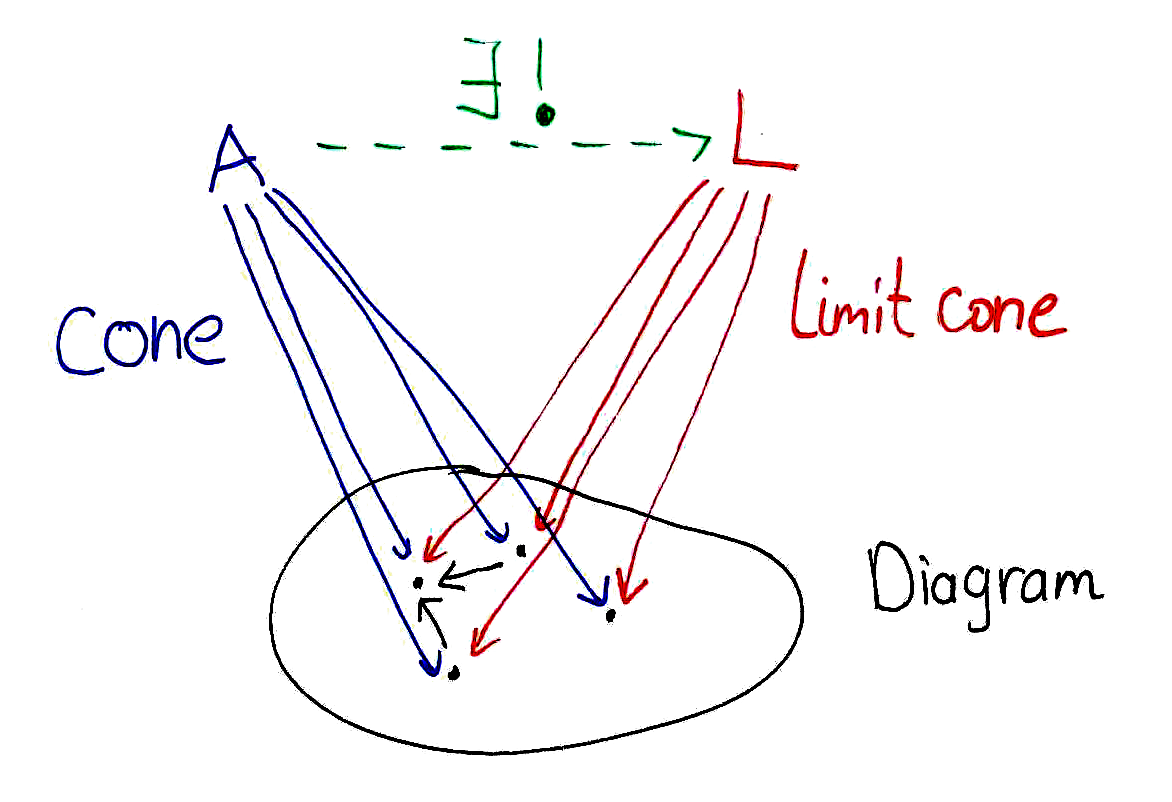
\includegraphics[scale=0.15]{Images/limits.png}
    \caption{Limit as the terminal cone over a diagram.}
    \label{fig:limits}
\end{figure}
    
\begin{example}
\begin{enumerate}
    \item $\calJ=\varnothing$ and $F$ is the empty functor into $\calC$. Then $\limit(F)$ is a terminal object in $\calC$ and $\colimit(F)$ is an initial object in $\calC$.
    \item $\calJ=(\bullet\quad\bullet)$ (discrete category with two objects). Then $\limit(F)=F(1)\times F(2)$ and $\colimit(F)=F(1)\sqcup F(2)$.
    \item $\calJ=(A\bullet\to \bullet_D\longleftarrow \bullet B$, then $\limit(F)=A\times_D B$.
    \item $F(\calJ)=(A\bullet\to \bullet B)$, then $\limit(F)=A$ and $\colimit{F}=B$.
    \item $F(\calJ)=(A\bullet\toto[\alpha]{\beta}\bullet B)$. Then $\limit(F)=\mathrm{eq}(\alpha,\beta)=\{a\mid \alpha(a)=\beta(a)\}$ is the equalizer and $\colimit(F)=\mathrm{coeq}(\alpha,\beta)=B/(\alpha(a)\sim \beta(a))$ is the coequalizer.

\end{enumerate}
\end{example} 

The most common examples of infinite limits and colimits are ones where $\mathcal{J}$ can be indexed by integers.

\begin{defn}[Direct and inverse limits]\index{Limit!direct}\index{Limit!inverse}
    If $\calJ=(\bullet\to\bullet\to\bullet\to\cdots)$, then $\colimit(F)$ is called a direct, or an inductive, limit. It is also often written as $\colimit A_j$, where $A_j=F(j)$.
    
    If $\calJ=(\cdots\to\bullet\to\bullet\to\bullet)$, then $\limit(F)$ is called an inverse, or a projective, limit.
    
    More generally, if $\calJ$ is a poset category (see Example \ref{poset example}), then it is said to be directed to the right (left) if $\forall i,j\in \ob(\calJ)$ $\exists k\in \ob(\calJ)$ such that $i,j\leq k$ (respectively, $k\leq i,j$). Then one can define direct limits of diagrams directed to the right and inverse limits of diagrams directed to the left.
\end{defn}


\begin{example}
\begin{enumerate}
    \item In $\colimit$, most commonly all arrows are monomorphisms. For example, consider the category $\mathsf{Gr}$ of groups and the sequence $S_n$ of symmetric groups with the embeddings $S_n\hookrightarrow S_m$ for every $n<m$ defined as permutations of the first $n$ symbols. Then $\colimit(S_n)=S_\infty$, which is the group of all permutations of $\mathbb{N}$ of finite support.
    
    Alternatively, we can define another partial order on the set of symmetric groups $S_n$. Namely, define $n\preccurlyeq m\Leftrightarrow n\mid m$ and the inclusion $S_n\hookrightarrow S_m$ by $m/n$ copies of the permutation. Then $\colimit (S_n)$ is a different group.
    \item For any unital ring $R$, the direct limit of the general linear matrix groups over $R$ (where matrices of size $n$ are embedded into groups of larger matrices by filling in the diagonal with ones) is $\colimit(\GL(n,R))=\GL(R)$, the \emph{quite general linear group} of $R$.
    \item In $\mathsf{Set}$, direct limits are simply infinite unions factored by identifying elements with coincident ``descendants'', i.e. $\colimit A_i=\bigsqcup_i A_i/\sim$, where $x\in A_i$ is equivalent to $y\in A_j$ iff $\exists f_{jk},f_{jk}$ such that $f_{ik}(x)=f_{jk}(y)$. The inverse limit is the set of infinite sequences of descendants $\limit (A_i)=\{(a_i)\mid a_i\in A_i,\forall i\leq j, f_{ij}(a_i)=a_j\}$.
    \item Consider the polynomial ring $K[t]$ over a field $K$ and its factor rings $K[t]/t^n$ of truncated polynomials. Then we have the sequence of epimorphisms 
    \[\cdots \to K[t]/t^3\to K[t]/t^2\to K,\]
    and the inverse limit is $\limit(K[t]/t^n)=K[[t]]$, which is the ring of \emph{all} formal power series $\sum_{i\geq 0}a_i t^i$. This illustrates the more general fact that projective limits are generally enormous, so much so that the cardinality of the limit is often higher than of any object in the sequence.
    \item Let $p$ be a prime integer and consider the sequence of groups
    \[\cdots\to \mathbb{Z}/p^3 \mathbb{Z}\overset{\mod p^2}\to \mathbb{Z}/p^2\mathbb{Z}\overset{\mod p}\to \mathbb{Z}/p\mathbb{Z}.\]
    Then $\limit(\mathbb{Z}/p^n\mathbb{Z})=\mathbb{Z}_p$ is the group of $p$-adic integers (it has the cardinality of continuum!).
    \item Consider the poset diagram directed to the left consisting of group epimorphisms $\mathbb{Z}/m\mathbb{Z}\overset{\mod n}\to \mathbb{Z}/n\mathbb{Z}$ for $n\mid m$. Then 
    $\limit (\mathbb{Z}/n\mathbb{Z})=\hat{\mathbb{Z}}$ is the \emph{profinite completion of $\mathbb{Z}$}.
    \item The monomorphism sequence $\mathbb{Z}/p^n\mathbb{Z}\overset{\cdot p}\to \mathbb{Z}/p^{n+1}\mathbb{Z}$ gives the direct limit $\colimit(\mathbb{Z
    }/p^n\mathbb{Z})=\mathbb{Z}(p^\infty)$, which is called a Pr\"ufer group (it can be realized as the group of all roots of unity of the form $\exp(2\pi i\cdot m/p^n)$).
    \item In topological and geometric categories, direct limits are similar to unions (when they exist). For instance, the $n$-sphere can be embedded $S^n\hookrightarrow S^{n+1}$ as the equator, and the direct limit gives $S^\infty=\colimit S^n$.
\end{enumerate}
\end{example}
\begin{xca}
    Show that $S^\infty$ is contractible (unlike any finite-dimensional sphere).
\end{xca}



\subsection{Sub-objects and Quotient Objects}

\begin{defn}
    Let $X,U,V\in\ob(\calC)$ and consider a diagram
    \[\begin{tikzcd}[every matrix/.append style={name=m},   
        execute at end picture={\draw [<-] ([xshift=-2mm,yshift=-12mm]m-1-2.north) arc[start angle=-90,delta angle=-270,radius=0.25cm];}]
        U \arrow[dr,tail,"u\text{, mono}"]& \\
        & X\\
        V\arrow[uu,tail,dashed,"\exists h"]\arrow[ur,tail,swap,"v\text{, mono}"]& 
\end{tikzcd}\]
    We say that $v\leq u$ if there exists a morphism $h$ such that $v=u\circ h$ ($h$ has to be a monomorphism for this to hold).
\end{defn}

Here are the properties of this relation:
\begin{enumerate}
    \item $u\leq u$;
    \item $u\leq v,v\leq w\Rightarrow u\leq w$;
    \item $u\leq v,v\leq u\Rightarrow U\overset{f}{\cong} V$, where $u=v\circ f$ and $v=u\circ f^{-1}$.
    \begin{proof}
        We have $V\overset{h}{\to}U$ and $U\overset{g}{\to}V$.
        
        On the one hand, $v=u\circ h=v\circ g\circ h\Rightarrow g\circ h=1_V$ since $v$ is mono.
        
        On the other hand, $u=u\circ(h\circ g)\Rightarrow h\circ g=1_U$ since $u$ is mono.
    \end{proof}
\end{enumerate}

\begin{defn}[Sub-objects]\index{Sub-object}
    Introduce an equivalence relation on monomorphisms: $u\sim v$ iff $u\leq v$ and $v\leq u$. Then a sub-object of $X$ is an equivalence class of pairs $(U,u)$, where $u:U\to X$ is a mono.
\end{defn}

\begin{example}
    $\mathbb{Z}\overset{\cdot n}\to \mathbb{Z}$ is mono and defines the group $n\mathbb{Z}$ as a sub-object of $\mathbb{Z}$.
\end{example}

\begin{defn}[Quotient objects]\index{Quotient object}
    For epimorphisms, we define the relation $y\geq z$ if in the diagram 
    \[\begin{tikzcd}[every matrix/.append style={name=m},   
        execute at end picture={\draw [<-] ([xshift=-6mm,yshift=-5mm]m-2-2.north) arc[start angle=-90,delta angle=-270,radius=0.25cm];}]
        & Y \arrow[dd,two heads,dashed,"\exists h"] \\
        X\arrow[dr,two heads,swap,"z\text{, epi}"]\arrow[ur,two heads,"y\text{, epi}"] &\\
        & Z 
    \end{tikzcd}\]
    there exists such a morphism $h$ that $z=h\circ y$ (it has to be epi).
    Then a quotient object of $X$ is an equivalence class of pairs $(Y,y)$, where $y:X\to Y$ is epi.
\end{defn}

\begin{example}
    There are many different epimorphisms $\mathbb{Z}^2\to\mathbb{Z}$. They define many non-equivalent quotient objects of $\mathbb{Z}^2$, each isomorphic to $\mathbb{Z}$.
\end{example}



\subsection{Abelian Categories}

Abelian categories are, roughly speaking, categories where objects and morphisms form Abelian groups themselves, and where the First Isomorphism theorem holds. Examples include $\mathsf{Ab}$, $\mathsf{Vect}_K$, $R-\mathsf{Mod}$ or $\mathsf{Mod}-R$, $\mathsf{SheafAb}$. Notably, $\mathsf{TopAb}$ is not Abelian because the First Isomorphism theorem generally doesn't hold for topological groups (we call such a category pre-Abelian).

\begin{defn}[Abelian categories]\index{Abelian category}
    A category $\calC$ is called Abelian if:
    \begin{enumerate}
        \item Every morphism set $\mor(A,B)$ has the structure of an Abelian group, i.e. morphisms can be added and subtracted.
        \item There exists a zero object $0\in\ob(\calC)$.
        \item The product and coproduct of any two objects exist and are isomorphic. The result is denoted by the direct sum: $A\times B\cong A\sqcup B \equiv A\oplus B$.
        \item All equalizers and coequalizers exist. In particular, using the Abelian property, we define
        \[\ker (\varphi)\coloneqq\mathrm{eq}(\varphi,0),\quad \coker(\varphi)\coloneqq\mathrm{coeq}(\varphi,0).\]
        \item The image and coimage of any morphism coincide, $\im (\varphi)=\coim(\varphi)$. These will be defined below.
    \end{enumerate}
\end{defn}

We can give alternative definition of kernels and cokernels.
\begin{defn}[Kernel]\index{Kernel}
    Let $X\overset\varphi\to Y$ be a morphism in an Abelian category. Then $\ker\varphi$ is the sub-object $(K,k)$ of $X$ such that $\varphi\circ k=0$ and it is universal with this property:
    \[\begin{tikzcd}[every matrix/.append style={name=m},   
        execute at end picture={\draw [<-] ([xshift=-10mm,yshift=-8mm]m-1-2.north) arc[start angle=-90,delta angle=-270,radius=0.15cm];}]
        K \arrow[r,tail,"k"]& X\arrow[r,"\varphi"] & Y\\
        Z\arrow[u,dashed,"\exists! h"]\arrow[ur,swap,"\forall\psi:\,\varphi\circ\psi=0"]& & 
    \end{tikzcd}\]
    (such a $h$ is automatically unique for every $\psi$ because $k$ is mono).
\end{defn}

\begin{defn}[Cokernel]\index{Cokernel}
    Let $X\overset\varphi\to Y$ be a morphism in an Abelian category. Then $\coker\varphi$ is the quotient object $(C,c)$ of $Y$ such that $c\circ\varphi=0$ and it is universal with this property:
    \[\begin{tikzcd}[every matrix/.append style={name=m},   
        execute at end picture={\draw [<-] ([xshift=-4mm,yshift=-8mm]m-1-3.north) arc[start angle=-90,delta angle=-270,radius=0.15cm];}]
        X\arrow[r,"\varphi"] & Y \arrow[r,two heads,"c"]\arrow[dr,swap,"\forall\psi:\,\psi\circ\varphi=0"]  & C\arrow[d,dashed,"\exists! h"] \\
        & & Z
    \end{tikzcd}\]
    (such a $h$ is automatically unique for every $\psi$ because $c$ is epi).
\end{defn}

\begin{example}
    It is easy to check that in the category $\mathsf{Ab}$ of Abelian groups, $\coker\varphi=H/\varphi(G)$ for $\varphi:G\to H$. Thus the last axiom of Abelian categories is equivalent to the First Isomorphism theorem in this case. Note that this factor doesn't exist neither in $\mathsf{Gr}$ nor in $\mathsf{TopAb}$.
    
    The same formula holds for all ring modules. In $\mathsf{Gr}$ (which is not an Abelian category, but in which kernels and cokernels can be similarly defined), the cokernel is the quotient by the normal closure of the image.
\end{example}

This allows us to define images and coimages.

\begin{defn}[Image, coimage]\index{Image of a morphism}\index{Coimage of a morphism}
    In Abelian categories, $\im\varphi$ for a morphism $\varphi:X\to Y$ is the sub-object of $Y$ defined as
    \[\im(\varphi)=\ker(\coker\varphi),\quad\quad K\overset k \rightarrowtail X\overset\varphi\to Y\overset c\twoheadrightarrow C.\]
    Similarly, $\coim\varphi$ is the quotient object of $X$ defined as 
    \[\coim(\varphi)=\coker(\ker\varphi).\]
\end{defn}

Note that
\[\ker(\coim\varphi)=\ker(\coker(\ker\varphi)))=\im(\ker\varphi).\]
Thus in general pre-Abelian categories (i.e.\ without the last axiom) by the universal properties of images and coimages we have a factorization of any morphism $\varphi:X\to Y$ into the sequence
\[\ker\varphi\rightarrowtail X\underbrace{\overset{\text{epi}}\twoheadrightarrow\coim\varphi\overset{\text{bi}}\to\im\varphi\overset{\text{mono}}\rightarrowtail}_\varphi Y\twoheadrightarrow\coker\varphi \]
The last axiom of Abelian categories states that $\coim\varphi\cong \im\varphi$, which is equivalent to the statement:
\[\boxed{\text{5. All bimorphisms are isomorphisms.}}\]
\begin{xca}
    Prove that the last axiom of Abelian categories is indeed equoivalent to the boxed statement.
\end{xca}
Therefore only in Abelian categories we have the decomposition
\[\ker\varphi\to X \overset{j\text{, epi}}\longrightarrow\im\varphi\overset{i\text{, mono}}\longrightarrow Y\to \coker\varphi,\]
where
\[\text{factorization property}:\quad \varphi=i\circ j,\quad i\text{ -- mono}, j\text{ -- epi}.\]

\begin{defn}[Additive functor]
    A functor $F:\calC\to\calD$ between two Abelian categories is called additive if for any $A,B\in\ob(\calC)$, the map $F_{A,B}:\Hom_\calC(A,B)\to \Hom_\calD(F(A),F(B))$ defined by $\varphi\mapsto F_{A,B}(\varphi)=F(\varphi)$ is a homomorphism of Abelian groups.
\end{defn}

The following theorem is the main general result about Abelian categories and effectively states that all Abelian categories can be realized as (almost arbitrarily nice) full subcategories of categories of ring modules. It is essentially a much stronger version of the Yoneda lemma \ref{Yoneda} for Abelian categories.

\begin{thm}[Freyd-Mitchell]
    For any Abelian category $\calC$ there exists a ring $R$ and a functor $F:\calC\to R\text{-}\mathsf{Mod}$ that is: additive, full and faithful (surjective and injective on sets of morphisms for each pair of objects), preserves kernels, cokernels, products and coproducts, is exact (preserves exact sequences, see below)...
\end{thm}
This theorem justifies all diagrammatic methods that we will develop in the next two sections: since $R\text{-}\mathsf{Mod}$ is a concrete category, its objects are sets. Therefore by the Freyd-Mitchell theorem, it suffices to prove any general statement about Abelian categories only for categories of ring modules, which allows us to refer to elements of objects as sets, and apply morphisms as functions to those elements!


\subsection{Exact Sequences and Functors}

From now on in this Part we work only with Abelian categories.
\begin{defn}[Exact sequences]\index{Exact sequence}
 A sequence of morphisms in an Abelian category 
 \[\cdots \to A_{i-1}\overset{\alpha}\to A_i\overset{\beta}\to A_{i+1}\to \cdots\]
 is called exact in $A_i$ if 
 \[\im\alpha=\ker\beta.\]
 A sequence is just called exact if it is exact in every object in it.
\end{defn}

\begin{prop}
    \begin{enumerate}
        \item A sequence $0\to A\overset f\to B$ is exact iff $f$ is mono;
        \item A sequence $A\overset f\to B\to 0$ is exact iff $f$ is epi;
        \item A sequence $0\to A\overset f\to B\to 0$ is exact iff $f$ is an isomorphism;
        \item A sequence $0\to A\to B\overset f\to C\to D\to 0$ is exact iff $A=\ker f$ and $D=\coker f$.
    \end{enumerate}
\end{prop}
\begin{proof}
    Exercise.
\end{proof}

\begin{defn}[Short exact sequences]\index{Exact sequence!short}
 A short exact sequence is an exact sequence of the form
 \[0\to A\overset f\rightarrowtail B\overset g \twoheadrightarrow C\to 0.\]
 Such a sequence (and the object $B$ in particular) is also called an \emph{extension} of $A$ by $C$. The exactness of this sequence is equivalent to $f$ being mono, $g$ being epi, and $\im f=\ker g$.
\end{defn}

\begin{prop}[First isomorphism theorem]
    If $0\to A\overset f\to B\overset g \to C\to 0$ is a short exact sequence, then 
    \[A\cong \im f,\quad C\cong B/\im f.\]
\end{prop}
\begin{proof}
    The first isomorphism is known in concrete categories, which is sufficient. It states that $B/\ker g\cong \im g$, and by exactness $\ker g=\im f$ and $\im g=C$, thus $B/\im f\cong C$.
\end{proof}

\begin{defn}[Split sequence]\index{Split sequence}
 A short exact sequence $0\to A\overset i\to B\overset p \to C\to 0$ is called split if there exists a morphism $j:C\to B$ with $p\circ j=1_C$, i.e. if $p$ is a split epi.
\end{defn}

\begin{prop}[Rank-nullity theorem]\index{Rank-nullity theorem}
    If a short exact sequence $0\to A\overset i\to B\overset p \to C\to 0$ is split, then $B\cong A\oplus C$.
\end{prop}
\begin{proof}
    We show that $B\cong \im i\oplus \im j$, where $j$ is a section for $p$. We perform a simple \emph{diagram chasing} by considering an element $b\in B$:
    \[b\in B\implies p(b-j\circ p(b))=p(b)-\underbrace{p\circ j}_{1_C}(p(b))=0\implies b-j\circ p(b)\in\ker p\overset{\text{exact}}{\implies}\exists a\in A: i(a)=b-j\circ p(b).\]
    This proves that $B=\im i+\im j$. To prove that $\im i\cap \im j=\{0\}$, suppose $x=i(a)=j(c)$. Then $p(x)=p(i(a))=0$ since $p\circ i=0$, and at the same time $p(x)=p(j(c))=c$ since $p\circ j=1_C$. Thus $c=0$, $x=j(c)=0$, and $B\cong A\oplus C$.
\end{proof}

\begin{prop}[Rank-nullity for vector spaces]\label{gen rank-nullity}
    If $0\to A_1\overset{f_1}\to A_2 \overset{f_2}\to\cdots A_n\to 0$ is an exact sequence of finite dimensional vector spaces, then
    \[\sum_{i=1}^n(-1)^i \dim A_i=0.\]
\end{prop}
\begin{proof}
    By the standard rank-nullity theorem, the l.h.s.\ equals \[\sum_{i=1}^{n-1}(-1)^i\dim \ker f_i+\sum_{i=1}^{n-1}(-1)^i\dim \im f_i.\] By exactness, this sum vanishes.
\end{proof}


\begin{comment}
    \begin{samepage}
        \PRLsep
        \begin{center}
            {\red Lecture 19 on 26 Apr 2019 ended here}
        \end{center}
    \end{samepage}
\end{comment}



\begin{defn}[Exact functors]\index{Exact functor}
 A functor $F:\calC\to\calD$ is called exact if it maps every exact sequence into an exact sequence.
\end{defn}

\begin{prop}
    For an additive functor $F$, exactness follows from exactness only on short sequences.
\end{prop}
\begin{proof}
    The idea of the proof is to expand any segment of an exact sequence $A\to B\to C$ into a combination of short exact sequences (this method is generally called ``splicing'' of short sequences).
    
    Namely, we have the following \emph{commutative} diagram with exact diagonals:
    \[\begin{tikzcd}
        0 \arrow[dr]& & & & 0 \arrow[dr]& & 0 & & \\ 
        & \ker f \arrow[dr]&&&& \im g \arrow[dr]\arrow[ur]&&&\\
        && A \arrow[rr,"f"]\arrow[dr]&& B \arrow[rr,"g"]\arrow[ur] && C \arrow[dr] &&\\
        &&& \im f\arrow[dr]\arrow[ur] &&&& \coker g\arrow[dr]&\\
        && 0 \arrow[ur] && 0 &&&& 0
    \end{tikzcd}\]
    Applying $F$, we get the \emph{commutative} diagram
    \[\begin{tikzcd}
        0 \arrow[dr]& & & & 0 \arrow[dr]& & 0 & & \\ 
        & F(\ker f) \arrow[dr]&&&& F(\im g) \arrow[dr]\arrow[ur]&&&\\
        && F(A) \arrow[rr,"F(f)"]\arrow[dr]&& F(B) \arrow[rr,"F(g)"]\arrow[ur] && F(C) \arrow[dr] &&\\
        &&& F(\im f)\arrow[dr]\arrow[ur] &&&& F(\coker g)\arrow[dr]&\\
        && 0 \arrow[ur] && 0 &&&& 0
    \end{tikzcd}\]
    with exact diagonals. Now we notice
    \begin{multline}
        \im F(f)=\im\left(F(A)\to F(\im f)\to F(B)\right)=\im(F(\im f)\to F(B))=\\
        =\ker (F(B)\to F(\im g))=\ker (F(B)\to F(\im g)\to F(C))=\ker F(g),
    \end{multline}
    where the second equality follows from $F(A)\to F(\im f)$ being epi and the next to last equality holds since $F(\im g)\to F(C)$ is mono. Therefore $F(A)\to F(B)\to F(C)$ is exact.
\end{proof}

There are in fact very few exact functors. Here are a few relevant examples.

\begin{example}
    \begin{enumerate}
        \item Let $G\text{-}\mathsf{Ab}$ be the category of Abelian groups with a $G$-action (morphisms in it are equivariant homomorphisms $f(g\cdot a)=g\cdot f(a)$). Then we can define the functor that for every group $A$ with a $G$-action produces its subgroup of invariants $A^G$:
        \[A^G=\{a\in A\mid \forall g\in G,\; g\cdot a=a\}.\]
        (The action on morphisms is trivial.) This is a functor $G\text{-}\mathsf{Ab}\to\mathsf{Ab}$. Now let us consider a short exact sequence
        \[0\to A\to B\to B/A\to 0.\]
        Its image is clearly not exact on the right:
        \[0\to A^G\to B^G\to (B/A)^G \cancel{\to} 0.\]
        Indeed, $(B/A)^G$ are $G$-invariant only up to addition of elements of $A$, whereas $B^G/A^G$ (which is what we would have in a short exact sequence) is a totally different group consisting of classes of truly $G$-invariant elements. We say that this functor is only \emph{left exact}.
        \item The representable (hom-)functors $\Hom_{R\text{-}\mathsf{Mod}}(\_,\_)$ acting $R\text{-}\mathsf{Mod}\times R\text{-}\mathsf{Mod}\to \mathsf{Ab}$ with either argument fixed can act on a short exact sequence 
        \[0\to A\to B\to C\to 0\]
        to give two exact sequences
        \begin{eqnarray}
            0\to \Hom(X,A)\to \Hom(X,B)\to \Hom(X,C),\\
            0\to \Hom(C,Y)\to \Hom(B,Y)\to \Hom(A,Y).
        \end{eqnarray}
        Therefore Hom-functors are also only left exact. Indeed, right exactness for them would mean that every morphism $X\to C$ or $A\to Y$ can be factored through $B$, which we know to be false. For example, consider
        \[\begin{tikzcd}
        0\arrow[r]& A=\mathbb{Z}\arrow[r,"\text{incl.}"]\arrow[d,
        "\id"]& B=\frac{1}{n}\mathbb{Z}\arrow[dl,dashed,"?"] \\
         &Y=\mathbb{Z} &
        \end{tikzcd}\]
        For right exactness, $\id:A\to Y$ would need to factor through $B$, which is clearly impossible here.
        
        An analogous example for the first line is
        \[\begin{tikzcd}
        B=\mathbb{Z}\arrow[r,"\mod n"] & C=\mathbb{Z}/n\mathbb{Z}\arrow[r] & 0 \\
         &X=\mathbb{Z}/n\mathbb{Z}\arrow[ul,dashed,"?"]\arrow[u,
        "\id"] &
        \end{tikzcd}\]
        If this functor were to be surjective on Hom-sets, every map $X\to C$ would have to come from a map $X\to B$, which is clearly false in this case.
        \item The tensor product functor $\_\otimes\_:\mathsf{Mod}\text{-}R\times R\text{-}\mathsf{Mod}\to \mathsf{Ab}$ is also not exact. In fact it is only \emph{right exact}: for every short exact sequence
        \[0\to A\to B\to C\to 0\]
        it gives two exact sequences (in fact they are the same because $X\otimes Y$ is naturally isomorphic to $Y\otimes X$)
        \begin{eqnarray} 
        X\otimes A\to X\otimes B\to X\otimes C\to 0,\\
        A\otimes Y\to B\otimes Y\to C\otimes Y\to 0.
        \end{eqnarray}
        We will give an example that shows that this functor is not left exact in Example \ref{non-flat module example}.
    \end{enumerate}
\end{example}

\begin{defn}[Projective and injective objects]\index{Projective object}\index{Injective object}
    If the functor $\Hom(X,\_)$ is exact, $X$ is called a projective object (i.e.\ all morphisms $X\to C$ factor through $B$ in any exact sequence $B\to C\to 0$). If $\Hom(\_,Y)$ is exact, $Y$ is called an injective object (all morphisms $A\to Y$ factor through $B$ in any exact sequence $0\to A\to B$).
\end{defn}

\begin{defn}
    An object $X$ is called \emph{flat} if the functor $X\otimes\_$ (or equivalently $\_\otimes X$) is left exact.
\end{defn}

\begin{example}\label{non-flat module example}
    Consider in the category of $\mathbb{Z}$-modules the sequence on the left and its image under a tensor product with $\mathbb{Z}/n\mathbb{Z}$
    \[0\to \mathbb{Z}\overset{\cdot n}\to \mathbb{Z} \quad \overset{\otimes\mathbb{Z}/n\mathbb{Z}}\rightsquigarrow \quad \mathbb{Z}\otimes \mathbb{Z}/n\mathbb{Z}\overset{\cdot n}\to\mathbb{Z}\otimes \mathbb{Z}/n\mathbb{Z}.\]
    The arrow on the right is obviously not mono (it is the zero morphism), therefore $\mathbb{Z}/n\mathbb{Z}$ is not a flat $\mathbb{Z}$-module.
\end{example}

The moral of these examples is that whereas in categories of vector spaces $\mathsf{Vect}_K$ everything would be exact, exactness is generically broken as soon as we pass to structures over rings. The study of ring modules is a natural extension of linear (matrix) algebra over fields, and largely reduces to homological algebra.
\[
\boxed{\begin{array}{c}
\text{The goal of homological algebra is:}\\
\text{to study the obstructions to the exactness of additive functors (these obstructions are called derived functors).}
\end{array}}
\]
Given a non-exact functor, the values of its derived functors need to be added into the image of a short exact sequence to produce a fully exact (albeit potentially infinitely long) sequence. For example, in the case of the invariants functor, every short exact sequence $0\to A\to B\to B/A\to 0$ becomes a \emph{long exact sequence of group cohomology}
\[0\to A^G\to B^G\to (B/A)^G\to H^1(G,A)\to H^1(G,B)\to H^1(G,B/A)\to H^2(G,A)\to\cdots\]
For the Hom functor, the obstruction to right exactness is evaluated by the Ext-functors (the name comes from ``extension''):
\begin{gather}
    0\to \Hom(X,A)\to \Hom(X,B)\to\Hom(X,C)\to \Ext^1(X,A)\to \Ext^1(X,B)\to\Ext^1(X,C)\to\cdots,\\
    0\to \Hom(C,Y)\to \Hom(B,Y)\to\Hom(A,Y)\to \Ext^1(C,Y)\to \Ext^1(B,Y)\to\Ext^1(A,Y)\to\cdots
\end{gather}
Finally, for the tensor functor, the obstruction to left exactness is evaluated by the Tor-functors (``torsion''):
\[\cdots\to \Tor_2(C,X)\to \Tor_1(A,X)\to \Tor_1(B,X)\to\Tor_1(C,X)\to A\otimes X\to B\otimes X\to C\otimes X\to 0.\]
All of them are examples of (co)homology theories. We will return to a proper discussion of these objects later. The takeaway so far should be: since on manifolds we are studying spaces of sections of vector bundles, which are really $C^\infty(M)$-modules, we need homological algebra to deal with the linear algebra over the ring of functions, and the (co)homology groups will measure the non-exactness of certain constructions.




\subsection{Diagram Chasing Lemmas}

All of the following lemmas hold in arbitrary Abelian categories. Moreover, for every general diagrammatic statement in an Abelian category, its dual holds as well (i.e.\ the diagram with all arrows reversed), since we can always pass to the dual category, which is also Abelian.

\begin{lem}
    If the square 
    \[\begin{tikzcd}[every matrix/.append style={name=m},   
        execute at end picture={\draw [<-] ([xshift=-7mm,yshift=-10mm]m-1-2.north) arc[start angle=-90,delta angle=-270,radius=0.25cm];}]
        A_1 \arrow[r,"\phi"]\arrow[d,"\pi"] & B_1\arrow[d,"\rho"] \\
        A_2\arrow[r,"\psi"] &B_2 
    \end{tikzcd}\]
    commutes, then there exist two morphisms $\eta:\ker\pi\to\ker\rho $ and $\theta:\coker\pi\to\coker\rho$ such that
    \[\begin{tikzcd}[every matrix/.append style={name=m},   
        execute at end picture={\draw [<-] ([xshift=-11mm,yshift=1mm]m-2-2.north) arc[start angle=-90,delta angle=-270,radius=0.25cm];
        \draw [<-] ([xshift=-11mm,yshift=1mm]m-3-2.north) arc[start angle=-90,delta angle=-270,radius=0.25cm];
        \draw [<-] ([xshift=-11mm,yshift=1mm]m-4-2.north) arc[start angle=-90,delta angle=-270,radius=0.25cm];}]
        \ker\pi \arrow[r,"\eta"]\arrow[d] & \ker\rho \arrow[d] \\
        A_1\arrow[r,"\phi"]\arrow[d,"\pi"] &B_1\arrow[d,"\rho"]\\
        A_2\arrow[r,"\psi"]\arrow[d] &B_2\arrow[d]\\
        \coker\pi \arrow[r,"\theta"] & \coker\rho
    \end{tikzcd}\]
    in this diagram the columns, formed by the factorizations of $\pi$ and $\rho$, are exact (in fact, exact even after being augmented with zeros on both ends).
\end{lem}
\begin{proof}
    As usual, we only prove this for $R\text{-}\mathrm{Mod}$. Let $x\in \ker\pi\subset A_1$. Then $\rho(\phi(x))=\psi(\pi(x))=0$, so $\phi(x)\in\ker\rho$. Thus we define $\eta(x)\coloneqq\phi(x)$.
    
    For $\theta$, it is in fact enough to pass to the dual category, in which the existence of $\theta$ reduces to the above construction of $\eta$.
    
    Alternatively, let $x\in A_2/\im\pi$. Define the map \[A_2/\im\pi\to B_2/\im\rho,\quad x+\im\pi\mapsto \psi(x)+\im\rho,\]
    which is valid since $\im(\psi\circ\pi)=\im(\rho\circ\phi)\subset \im\rho$. 
    
    The commutativity of the resulting diagrams follows from the definitions.
\end{proof}

\begin{lem}[3-lemma]
    If the rows of the commutative diagram 
    \[\begin{tikzcd}[every matrix/.append style={name=m},   
        execute at end picture={\draw [<-] ([xshift=-7mm,yshift=-10mm]m-1-2.north) arc[start angle=-90,delta angle=-270,radius=0.2cm];
        \draw [<-] ([xshift=-7mm,yshift=-10mm]m-1-3.north) arc[start angle=-90,delta angle=-270,radius=0.2cm];}]
        A_1 \arrow[r,"f_1"]\arrow[d,"\pi"] & B_1\arrow[d,"\rho"]\arrow[r,"g_1"] & C_1\arrow[d,"\sigma"] \\
        A_2\arrow[r,"f_2"] &B_2 \arrow[r,"g_2"] &C_2 
    \end{tikzcd}\]
    are exact, then:
    \begin{enumerate}
        \item if $\sigma$ is mono, then $\im\rho\cap\im f_2=\im(f_2\circ \pi)=\im(\rho\circ f_1)$;
        \item if $\pi$ is epi, then $\ker\rho+\im f_1=\ker(g_2\circ\rho)=\ker(\sigma\circ g_1)$.
    \end{enumerate}
\end{lem}
\begin{proof}
    \begin{enumerate}
        \item The inclusion $\im(f_2\circ\pi)\subset \im\rho\cap \im(f_2)$ is obvious. Now let $x\in \im(\rho)\cap(\im(f_2)=\ker g_2)$. Then $\exists y\in B_1: \rho(y)=x$. Since $\im f_2=\ker g_2$, we have $g_2(\rho(y))=0=y\sigma(g_1(y))$, so $g_1(y)=0$ because $\sigma$ is mono. By the exactness of the top row, $y\in\im f_1$, therefore $\exists z\in A_1:f_1(z)=y$, thus $x=\rho(f_1(z))$ and $x\in\im(\rho\circ f_1)$.
        \item Pass to the dual category and reduce to the first part. Alternatively, the inclusion $\ker\rho+\im f_1\subset \ker(g_2\circ\rho)$ is obvious. Now assume $x\in \ker g_2\circ\rho$. By exactness, $\exists y\in A_2:f_2(y)=\rho(x)$. Since $\pi$ is epi, $\exists z\in A_1:y=\pi(z)$. Then $\rho(f_1(z))=f_2(\pi(z))=f_2(y)=\rho(x)$, which means that $f_1(z)$ and $x$ differ by an element of $\ker\rho$, which is what we sought to prove.
    \end{enumerate}
\end{proof}

\begin{lem}[5-lemma]\label{5-lemma}
    If the rows of the commutative diagram
    \[\begin{tikzcd}[every matrix/.append style={name=m},   
        execute at end picture={\draw [<-] ([xshift=-8mm,yshift=-10mm]m-1-2.north) arc[start angle=-90,delta angle=-270,radius=0.2cm];
        \draw [<-] ([xshift=-8mm,yshift=-10mm]m-1-3.north) arc[start angle=-90,delta angle=-270,radius=0.2cm];
        \draw [<-] ([xshift=-8mm,yshift=-10mm]m-1-4.north) arc[start angle=-90,delta angle=-270,radius=0.2cm];
        \draw [<-] ([xshift=-8mm,yshift=-10mm]m-1-5.north) arc[start angle=-90,delta angle=-270,radius=0.2cm];}]
        A_{-2}\arrow[r,"f_{-2}"]\arrow[d,"\pi_{-2}"] & A_{-1}\arrow[r,"f_{-1}"]\arrow[d,"\pi_{-1}"] & A_0 \arrow[r,"f_0"]\arrow[d,"\pi_0"] & A_1\arrow[d,"\pi_1"]\arrow[r,"f_1"] & A_2\arrow[d,"\pi_2"] \\
       B_{-2}\arrow[r,"g_{-2}"] & B_{-1}\arrow[r,"g_{-1}"] & B_0\arrow[r,"g_0"] &B_1 \arrow[r,"g_1"] &B_2 
    \end{tikzcd}\]
    are exact, then:
    \begin{enumerate}
        \item if $\pi_{-2}$ is epi and $\pi_{\pm 1}$ are mono, then $\pi_0$ is mono;
        \item if $\pi_2$ is mono and $\pi_{\pm 1}$ are epi, then $\pi_0$ is epi.
    \end{enumerate}
\end{lem}
\begin{proof}
    Let $x\in A_0$ be such that $\pi_0(x)=0$. We need to show that $x=0$. By commutativity, $g_0(\pi_0(x))=\pi_1(f_0(x))=0$, so $f_0(x)=0$ because $\pi_1$ is mono. By exactness, $\exists y\in A_{-1}:f_{-1}(y)=x$, and $g_{-1}(\pi_{-1}(y))=\pi_0(f_{-1}(y))=\pi_0(x)=0$. Then by exactness $\exists z\in B_{-2}:g_{-2}(z)=\pi_{-1}(y)$. Since $\pi_{-2}$ is epi, $\exists w\in A_{-2}:\pi_{-2}(w)=z$. Now 
    \[\pi_{-1}(y)=g_{-2}(\pi_{-2}(w))=\pi_{-1}(f_{-2}(w))\implies y=f_{-2}(w)\in\im f_{-2}=\ker f_{-1},\]
    since $\pi_{-1}$ is mono. Therefore $x=f_{-1}(y)=0$ by exactness.
\end{proof}
\begin{cor}
    \begin{enumerate}
        \item If $\pi_{-2}$ is epi, $\pi_2$ is mono, and $\pi_{\pm 1}$ are iso, then $\pi_0$ is iso;
        \item If the diagram
        \[\begin{tikzcd}[every matrix/.append style={name=m},   
        execute at end picture={\draw [<-] ([xshift=-8mm,yshift=-10mm]m-1-3.north) arc[start angle=-90,delta angle=-270,radius=0.2cm];
        \draw [<-] ([xshift=-8mm,yshift=-10mm]m-1-4.north) arc[start angle=-90,delta angle=-270,radius=0.2cm];}]
        0\arrow[r] & \bullet\arrow[r]\arrow[d,swap,"\pi_{-1}"] & \bullet \arrow[r]\arrow[d,swap,"\pi_0"] & \bullet\arrow[d,"\pi_1"]\arrow[r] & 0 \\
       0\arrow[r] & \bullet\arrow[r] & \bullet\arrow[r] &\bullet \arrow[r] &0
    \end{tikzcd}\]
    has exact rows and $\pi_{\pm 1}$ are both epi (mono), then $\pi_0$ is epi (respectively, mono).
    \end{enumerate}
\end{cor}

\begin{example}
    For any morphism $f:X\to Y$ we have the commutative diagram
    \[\begin{tikzcd}[every matrix/.append style={name=m},   
        execute at end picture={\draw [<-] ([xshift=-8mm,yshift=-10mm]m-1-3.north) arc[start angle=-90,delta angle=-270,radius=0.2cm];
        \draw [<-] ([xshift=-8mm,yshift=-10mm]m-1-4.north) arc[start angle=-90,delta angle=-270,radius=0.2cm];}]
        0\arrow[r] & \ker f \arrow[r]\arrow[d,swap,"0"] & X \arrow[r]\arrow[d,swap,"f"] & \coim f\arrow[d,"0"]\arrow[r] & 0 \\
       0\arrow[r] & \im f\arrow[r] & Y\arrow[r] &\coker f \arrow[r] &0
    \end{tikzcd}\]
    and its rows are exact by the definitions of (co)images and (co)kernels. The two zero morphisms $\ker f\overset{0}{\to} \im f$ and $\coim f\overset{0}{\to} \coker f$ are mono (epi) iff $f$ itself is mono (epi, respectively), which can be seen as an application of the 5-lemma.
\end{example}

\begin{lem}[4-lemma]
    If the rows of the commutative diagram
    \[\begin{tikzcd}[every matrix/.append style={name=m},   
        execute at end picture={\draw [<-] ([xshift=-8mm,yshift=-10mm]m-1-2.north) arc[start angle=-90,delta angle=-270,radius=0.2cm];
        \draw [<-] ([xshift=-8mm,yshift=-10mm]m-1-3.north) arc[start angle=-90,delta angle=-270,radius=0.2cm];
        \draw [<-] ([xshift=-8mm,yshift=-10mm]m-1-4.north) arc[start angle=-90,delta angle=-270,radius=0.2cm];}]
        A_1\arrow[r]\arrow[d,two heads,"\pi_1"] & A_2\arrow[r,"f"]\arrow[d,"\pi_2"] & A_3 \arrow[r]\arrow[d,"\pi_3"] & A_4\arrow[d,tail,"\pi_4"] \\
       B_1\arrow[r] & B_2\arrow[r,"g"] & B_3\arrow[r] &B_4
    \end{tikzcd}\]
    are exact, $\pi_1$ is epi, and $\pi_4$ is mono, then:
    \[\ker\pi_3=f(\ker\pi_2),\quad \im\pi_2=g^{-1}(\im \pi_3).\]
\end{lem}
\begin{proof}
    Exercise.
\end{proof}
\begin{cor}[Weak 4-lemma]
    In the above diagram, in addition:
    \begin{enumerate}
        \item if $\pi_3$ is epi, then so is $\pi_2$;
        \item if $\pi_2$ is mono, then so is $\pi_3$.
    \end{enumerate}
\end{cor}

\begin{lem}[Snake lemma/Connecting homomorphism lemma]\index{Snake lemma}\index{Connecting homomorphism}\label{snake lemma}
    Let the rows of the commutative diagram
    \[\begin{tikzcd}[every matrix/.append style={name=m},   
        execute at end picture={\draw [<-] ([xshift=-8mm,yshift=-10mm]m-1-3.north) arc[start angle=-90,delta angle=-270,radius=0.2cm];
        \draw [<-] ([xshift=-8mm,yshift=-10mm]m-1-4.north) arc[start angle=-90,delta angle=-270,radius=0.2cm];}]
        & A_0\arrow[r,"f_0"]\arrow[d,"\pi_0"] & A_1 \arrow[r,"f_1"]\arrow[d,"\pi_1"] & A_2\arrow[d,"\pi_2"]\arrow[r] & 0\\
       0\arrow[r] & B_0\arrow[r,"g_0"] & B_1\arrow[r,"g_1"] &B_2 & 
    \end{tikzcd}\]
    be exact. Then with the following diagram
    \[\begin{tikzcd}[background color=gray!20,every matrix/.append style={name=m},   
        execute at end picture={\draw [<-] ([xshift=-11mm,yshift=1mm]m-2-4.north) arc[start angle=-90,delta angle=-270,radius=0.25cm];
        \draw [<-] ([xshift=-11mm,yshift=-3mm]m-3-4.north) arc[start angle=-90,delta angle=-270,radius=0.25cm];
        \draw [<-] ([xshift=-11mm,yshift=1mm]m-5-4.north) arc[start angle=-90,delta angle=-270,radius=0.25cm];
        \draw [<-] ([xshift=-11mm,yshift=1mm]m-2-5.north) arc[start angle=-90,delta angle=-270,radius=0.25cm];
        \draw [<-] ([xshift=-11mm,yshift=3mm]m-4-5.north) arc[start angle=-90,delta angle=-270,radius=0.25cm];
        \draw [<-] ([xshift=-11mm,yshift=1mm]m-5-5.north) arc[start angle=-90,delta angle=-270,radius=0.25cm];}]
        & & \ker \pi_0 \ar{r}{\eta_0} \ar{d} & \ker \pi_1\ar{r}{\eta_1} \ar{d} &  \ker \pi_2 \ar{d}   %\arrow[ddll,"\delta",rounded corners
        & & \\
        &  &  A_0 \ar{r}{f_0} \ar{dd}[near start]{\pi_0} & A_1 \ar{r}{f_1} \ar{dd}[near start]{\pi_1} &  A_2\ar{r}\ar{dd}[near start]{\pi_2} & 0 &  ~\\[-1mm]
        & & &  ~ & & \ar[r, phantom, ""{coordinate, name=Y}] & ~\\[-3mm]
        ~&  \ar[l, phantom, ""{coordinate, name=Z}] 0 \ar{r} &  B_0 \ar{r}{g_0} \ar{d} &  B_1 \ar{r}{g_1} \ar{d} &  B_2 \ar{d} & &  \\
              & &  \ar[from=uuuurr, "\delta", dashed,crossing over, rounded corners,
                      to path=
                              { -- ([xshift=2ex]\tikztostart.east)
                              -| (Y) [near end]\tikztonodes
                              -| (Z) [near end]\tikztonodes
                              |- ([xshift=-2ex]\tikztotarget.west)
                               -- (\tikztotarget)}
                    ] \coker \pi_0\ar{r}{\theta_0}
               &  \coker \pi_1 \ar{r}{\theta_1}
               &  \coker \pi_2
               & 
               & 
    \end{tikzcd}\]
    there exists a unique \emph{connecting morphism}\index{Connecting morphism} $\delta$ shown in the diagram above which makes the kernel-cokernel sequence exact:
    \[\ker\pi_0 \to \ker\pi_1\to\ker\pi_2 \overset\delta\longrightarrow \coker\pi_0\to \coker\pi_1\to\coker\pi_2.\]

\end{lem}
\begin{proof}
    First one checks the exactness of the top and bottom rows of the large diagram using the 3-lemma.
    
    Next we construct $\delta$. Take $x\in \ker\pi_2\subset A_2$. Then $\exists y\in A_1:f_1(y)=x$ since $f_1$ is epi. By commutativity, $\pi_1(y)\in\ker g_1$, and by exactness, $\exists z\in B_0:g_0(z)=\pi_1(y)$. We define
    \[\delta(x)=z+\im \pi_0=[g_0^{-1}\circ\pi_1\circ f_1^{-1}(x)]\quad \in B_0/\im\pi_0=\coker\pi_0.\]
    Note that $z$ is uniquely determined by $y$ because $g_0$ is mono.
    
    Next we need to check correctness: given another $y': f_1(y')=x$, we have a unique $z':g_0(z')=\pi_1(y')$. One then shows that $z-z'\in \im\pi_0$.
    
    Moreover, we need to check that $\delta$ is a homomorphism (this is not completely obvious since the construction was not just a composition of homomorphisms).
    
    Finally, one checks the exactness of the resulting long sequence (in two terms, $\ker\pi_2$ and $\coker\pi_0$). We leave all these checks to the reader as an exercise.
\end{proof}


\begin{lem}[3$\times$3-lemma]\label{3x3-lemma}
    Let the rows of the commutative diagram
    \[\begin{tikzcd}[every matrix/.append style={name=m},   
        execute at end picture={\draw [<-] ([xshift=-7mm,yshift=-9mm]m-2-3.north) arc[start angle=-90,delta angle=-270,radius=0.2cm];
        \draw [<-] ([xshift=-7mm,yshift=-9mm]m-2-4.north) arc[start angle=-90,delta angle=-270,radius=0.2cm];
        \draw [<-] ([xshift=-7mm,yshift=-9mm]m-3-3.north) arc[start angle=-90,delta angle=-270,radius=0.2cm];
        \draw [<-] ([xshift=-7mm,yshift=-9mm]m-3-4.north) arc[start angle=-90,delta angle=-270,radius=0.2cm];}]
        &0\arrow[d]&0\arrow[d]&0\arrow[d]&\\
        0\arrow[r]& \bullet \arrow[r]\arrow[d] & \bullet\arrow[r]\arrow[d,"f"] & \bullet \arrow[r]\arrow[d] & 0\\
        0\arrow[r]& \bullet \arrow[r]\arrow[d] & \bullet\arrow[r]\arrow[d,"g"] & \bullet \arrow[r]\arrow[d] & 0\\
       0\arrow[r]& \bullet\arrow[r]\arrow[d] & \bullet\arrow[r]\arrow[d] & \bullet\arrow[r]\arrow[d] &0\\
       &0&0&0&
    \end{tikzcd}\]
    be exact. Then:
    \begin{enumerate}
        \item if the central and one of the side columns are exact, then the remaining column is exact too;
        \item if the two side columns are exact and the middle one is a \emph{complex}\index{Complex}, i.e.\ $g\circ f=0$, then the middle column is exact.
    \end{enumerate}
\end{lem}
\begin{proof}
    Exercise.
\end{proof}








\section{Cohomologies of Differential Forms}

\subsection{De Rham Cohomology}


\begin{defn}[de Rham cohomology]\index{Cohomology!de Rham}
    For a smooth manifold $M$, consider the sequence of vector spaces of differential forms, called the \emph{de Rham (cochain) complex},
    \[0\to\Omega^0(M)\overset\dd\to\Omega^1(M)\overset\dd\to\Omega^2(M)\to\cdots\]
    and define the spaces of closed forms, exact forms, and de Rham cohomology groups (in fact they are real vector spaces) respectively as
    \[Z^p=\ker\left(\restr{\dd}{\Omega^p(M)}\right),\quad B^p=\im\left(\restr{\dd}{\Omega^{p-1}(M)}\right),\quad H_{\rm dR}^p(M)=Z^p/B^p.\]
    This is possible because $d^2=0$, i.e.\ $B^p\subset Z^p$.
    Thus the sequence above is exact iff all de Rham cohomologies vanish.
\end{defn}
Thus de Rham cohomology counts non-exact closed differential forms.

\begin{prop}\label{prop zeroth cohomology}
    \begin{enumerate}
    \item If $M$ consists of $l$ connected components, then $H_{\rm dR}^0(M)=Z^0(M)=\bbR^l$.
    \item If $\dim M=n$, then $H_{\rm dR}^{> n}(M)=0$.
\end{enumerate}
\end{prop}
\begin{proof}
    Exercise.
\end{proof}

\begin{thm}[Poincar\'e lemma]\label{Poincare lem}
    $H^p_{\rm dR}(\mathbb{R}^{n})=H^{p}_{\rm dR}(\mathbb{R}^{n-1})$. More generally, for any manifold $M$,
    \[H^\bullet_{\rm dR}(M\times\bbR)=H^{\bullet}_{\rm dR}(M).\]
    By induction, $H^p_{\rm dR}(\mathbb{R}^{n})=0$ for $p>0$.
\end{thm}
\begin{proof}
    We present a proof from \cite{BottTu} that uses the general ideas of homotopy operators that will be useful to us later.
    
    Let $\pi:M\times\mathbb{R}\to M$ be the projection on the first factor and $s:M\to M\times\mathbb{R}^1$ the zero section (or in fact any section). Then we have the corresponding pullback maps on differential forms:
    \[\pi^\ast:\Omega^\bullet(M)\to \Omega^\bullet(M\times\bbR^1),\quad s^\ast: \Omega^\bullet(M\times\bbR^1)\to \Omega^\bullet(M).\]
    Note that $\pi\circ s=1$ and thus $s^\ast\circ\pi^\ast=1$. Also, both $s$ and $\pi$ send closed forms to closed forms, which means that they induce well-defined maps on corresponding cohomology groups, which we will denote by the same symbols.
    
    Let $x$ denote the points of $M$ and $t$ the points of $\bbR^1$. Every differential form on $M\times\bbR^1$ can be uniquely decomposed into a sub of the following types of forms:
    \[f(x,t)\cdot (\pi^\ast\omega),\quad f(x,t)\cdot(\pi^\ast\omega)\wedge\dd t,\]
    where $\omega$ is a form on $M$ and $f(x,t)$ is a real-valued function on $M\times\bbR$ with $x\in M$.
    
    Define the operator $K:\Omega^p(M\times\bbR^1)\to \Omega^{p-1}(M\times\bbR^1)$ by its action on the two kinds of forms from above,
    \[f\cdot \pi^\ast \omega\mapsto 0,\quad f\cdot\pi^\ast \omega \wedge\dd t\mapsto (\pi^\ast\omega)\int_0^t f.\]
    In other words, this operator integrates indefinitely over $\dd t$.
    
    Let us now show that $K$ is a \emph{homotopy operator} between $\pi^\ast\circ s^\ast$ and the identity, which means that
    \[\id-\pi^\ast\circ s^\ast=\pm (\dd K\pm K \dd),\]
    where the precise arrangements of signs is irrelevant.
    
    First let $\alpha=f(x,t)\cdot (\pi^\ast\omega)$ with $\deg \omega=p$ and compute
    \[(1-\pi^\ast s^\ast)\alpha=f(x,t)\pi^\ast\omega-f(x,0)\pi^\ast\omega,\]
    \[(\dd K-K \dd)\alpha=-K\dd\alpha=-K(f\dd\pi^\ast\omega+(-1)^p\dd f\wedge\pi^\ast\omega=(-1)^{p-1}\int_0^t\frac{\partial f}{\partial t}\pi^\ast\omega=(-1)^{p-1}(f(x,t)-f(x,0))\pi^\ast\omega.\]
    Therefore $(1-\pi^\ast s^\ast)\alpha=(-1)^{p-1}(\dd K-K \dd)\alpha$.
    
    Now, for forms of the second type, $\alpha=f(x,t)\cdot(\pi^\ast\omega)\wedge\dd t$, we have
    \[\dd\alpha=f\pi^\ast\dd\omega\wedge\dd t+(-1)^{p-1}\partial_x f\pi^\ast\omega\wedge\dd x\wedge\dd t,\]
    \[s^\ast\dd t=0\rightarrow (1-\pi^\ast s^\ast)\alpha=\alpha,\]
    \[K\dd \alpha=\left(\int_0^t f\right)\pi^\ast\dd\omega+(-1)^{p-1}\left(\int_0^t\partial_x f\right)\pi^\ast\omega\wedge\dd x,\]
    \[\dd K\alpha=\left(\int_0^t f\right)\pi^\ast\dd\omega+(-1)^{p-1}\left(\int_0^t\partial_x f\right)\pi^\ast\omega\wedge\dd x+(-1)^{p-1}f\pi^\ast\omega\wedge\dd t,\]
    so that
    \[(\dd K-K \dd)\alpha=(-1)^{p-1}\alpha.\]
    In all cases we find
     \[1-\pi^\ast\circ s^\ast=(-1)^{p-1}(\dd K\pm K \dd) \text{ on }\Omega^p(M\times\bbR).\]
     It turns out that having a homotopy operator immediately allows us to relate cohomologies of different degrees to each other. Indeed, $\dd K\pm K\dd$ maps closed forms to exact forms and therefore induces zero in cohomology (i.e.\ maps all cohomology equivalence classes to the trivial ones).
     In other words, the existence of such $K$ implies that 
     \[\pi^\ast\circ s^\ast=1 \text{ in }H^p_{\rm dR}(M).\]
     Therefore $\pi^\ast$ and $s^\ast$ are inverses of each other on cohomology:
     \[H^p_{\rm dR}(M\times\bbR)\cong H^p_{\rm dR}(M).\]
\end{proof}

\begin{cor}
    De Rham cohomology is a homotopy invariant. In other words, if two smooth maps $f,g:M\to N$ are homotopic, then their actions in cohomology coincide:
    \[f\sim g\implies f^\ast_{\rm dR}=g^\ast_{\rm dR}.\]
\end{cor}
\begin{proof}
    We have the homotopy $H:M\times[0,1]\to N$. Let $s_{0,1}:M\to M\times [0,1]$ be two constant sections given by $s_i(m)=(m,i),\;i=0,1$. Then $f=H\circ s_0$ and $g=H\circ s_1$. Their pullback actions are thus
    \[f^\ast=s_0^\ast H^\ast,\quad g^\ast=s_1^\ast H^\ast.\]
    However, we have shown in the proof of Poincar\'e lemma that $s_i^\ast=(\pi^\ast)^{-1}$ in de Rham cohomology (where $\pi:M\times [0,1]\to M$ is the projection), regardless of the specific section. Thus
    \[s_0^\ast=s_1^\ast\implies f^\ast=g^\ast \text{ in }H^\bullet_{\rm dR}.\]
\end{proof}


\subsection{Mayer-Vietoris Sequence}
\index{Sequence!Mayer-Vietoris}

Suppose $M=U\cup V$ with $U,V$ open. We have the inclusions
\[U\cap V\toto[i_1]{i_0}U\sqcup V\to M \]
Applying the contravariant functor $\Omega^\bullet$, we get the sequence of restrictions of forms
\[\Omega^\bullet(M)\to \Omega^\bullet(U)\oplus\Omega^\bullet(V)\toto[i_1^\ast]{i_0^\ast}\Omega^\bullet(U\cap V).\]
By taking the difference of the last two maps, we obtain the \emph{\gls{mv} sequence}\index{Mayer-Vietoris sequence}
\[0\to\Omega^\bullet (M)\to\Omega^\bullet(U)\oplus\Omega^\bullet(V)\overset{\text{difference}}\longrightarrow\Omega^\bullet (U\cap V)\to 0\]

\begin{prop}
    The \gls{mv} sequence is commutative (i.e.\ the horizontal maps introduced above commute with applications of $\dd$) and exact.
\end{prop}
\begin{proof}
    Commutativity is clear because $\dd$ is local and thus commutes with restrictions. The only nontrivial part is the surjectivity of the difference map. Consider a \gls{pou} $\{\chi_U,\chi_V\}$ subordinate to the open cover $\{U,V\}$ of $M$. Then any differential form $\omega\in\Omega^\bullet(U\cap V)$ can be decomposed as 
    \[\omega=\underbrace{\chi_U\omega}_{\Omega^\bullet(V)}-\underbrace{(-\chi_V)\omega}_{\Omega^\bullet(U)},\]
    which proves surjectivity.
\end{proof}

Consider a general exact sequence of differential complexes \[0\to A^\bullet\to B^\bullet\to C^\bullet \to 0,\] which is simply a shortened notation for the \emph{commutative} diagram
\[\begin{tikzcd}
        \; & \; & \; &\; &\; \\
        0 \arrow[r]& A^{p+1}\arrow[r,"f"]\arrow[u] &B^{p+1}\arrow[u]\arrow[r,"g"]& C^{p+1}\arrow[r]\arrow[u]& 0\\
       0\arrow[r] & A^p\arrow[r,"f"]\arrow[u,"d"] &B^p\arrow[u,"d"]\arrow[r,"g"]&C^p\arrow[u,"d"]\arrow[r]&0 \\
        &\arrow[u] & \arrow[u]& \arrow[u] &
\end{tikzcd}\]
in which every row is exact and $d^2=0$ in every column. The cohomology groups of each complex are again defined as $\ker d_{p}/\im d_{p-1}$. 

Essentially by the snake lemma \ref{snake lemma}, this induces a long exact sequence of cohomology groups:
\[\cdots\to H^p(A)\overset{f^\ast}\to H^p(B)\overset{g^\ast}\to H^p(C)\overset\delta\to H^{p+1}(A)\to H^{p+1}(B)\to H^{p+1}(C)\overset\delta\to H^{p+2}(A)\to \cdots\]
Namely, by surjectivity of $g$, for every closed $c\in C^p$, there exists a $b\in B^p$ such that $g(b)=c$. Using commutativity,  $g(\dd b)=\dd (gb)=\dd c=0$, and by exactness, there exists an $a\in A^{p+1}$ such that $\dd b=f(a)$. This $a$ is easily checked to be closed $\dd a=0$. Then we define $\delta([c])=[a]\in H^{p+1}(A)$. Some diagram chasing shows that this definition is independent of the choices made. We will discuss this sequence in detail later.

Applying this to the short \gls{mv} sequence, we obtain the \emph{long exact \gls{mv} sequence}
\[\cdots\to H^p(M)\to H^p(U)\oplus H^p(M)\to H^p(U\cap V)\to H^{p+1}(M)\to H^{p+1}(U)\oplus H^{p+1}(V)\to H^{p+1}(U\cap V)\to \cdots\]
Retracing the construction of the connecting homomorphism, we find that 
\[\delta^\ast([\omega])=
    \begin{cases}
        [-\dd (\chi_V \omega)],& \text{ on }U,\\
        [\dd (\chi_U \omega)],& \text{ on }V.
    \end{cases}
\]

\begin{example}[de Rham cohomology of $S^1$]\label{de Rham of circle}
    Let $M=S^1$ and let $U,V$ be a covering of the circle by two overlapping open arcs. Then we have the exact sequence
    \[0\to H^0(S^1)\overset\psi\to H^0(U\sqcup V)\overset\partial\to H^0(U\cap V)\overset\delta\to H^1(S^1)\to H^1(U\sqcup V)\to \cdots \]
    in which by Proposition \ref{prop zeroth cohomology} and Poincar\'e lemma \ref{Poincare lem}
    \[H^0(S^1)=\bbR,\quad H^0(U\sqcup V)=\bbR^2,\quad H^0(U\cap V)=\bbR^2,\quad H^1(U\sqcup V)=0,\]
    thus we get the exact sequence
    \[0\to \bbR\overset\psi\to \bbR^2\overset{\partial}\to \bbR^2\overset\delta\to H^1(S^1)\to 0,\]
    where
    \[\partial(a,b)=(a-b,a-b).\]
    Therefore by the rank-nullity theorem \ref{gen rank-nullity},
    \[1-2+2-\dim H^1(S^1)=0\Rightarrow H^1(S^1)=\bbR.\]
    Alternatively, we can compute it as follows
    \[\dim H^1(S^1)=\dim \im \delta=\dim \bbR^2-\dim\ker\delta=2-\dim\im \partial=2-(2-\dim\ker\partial))=\dim\ker\partial=\dim\im\psi =1\]
    since $\delta$ is surjective and $\psi$ is injective.
\end{example}


\begin{xca}
    Using the \gls{mv} sequence and homotopy invariance, show that $H_{\rm dR}^k(S^n)=H_{\rm dR}^{k-1}(S^{n-1})$ for $k\geq 2$, and by induction compute all de Rham cohomologies of any sphere $S^n$:
    \[n>0:\; H_p(S^n)=\begin{cases} \bbZ\,, & m=0,n\\ 0, & \text{otherwise.}\end{cases}\]
\end{xca}


\begin{xca}
    Using the homotopy invariance of de Rham cohomology, we can compute for example
    \[H^p_{\rm dR}(\bbR^n\setminus\{0\})=H^p_{\rm dR}(S^{n-1}),\]
    \[H^1_{\rm dR}(\text{M\"obius band})=H^1_{\rm dR}(S^1)=\bbZ.\]
\end{xca}


\begin{comment}
    \begin{samepage}
        \PRLsep
        \begin{center}
            {\red Lecture 20 on 3 May 2019 ended here}
        \end{center}
    \end{samepage}
\end{comment}

\subsection{De Rham Cohomology with Compact Support}

\begin{defn}[de Rham cohomology with compact support]\index{Cohomology!with compact support}
    Define $\Omega_c^\bullet(M)$ as the complex of differential forms with compact support on $M$. Then the cohomology groups $H_c^\bullet(M)$ of differential forms with compact support are defined just like before.
\end{defn}

\begin{prop}
    $\Omega_c^\bullet$ is not a functor with respect to arbitrary smooth maps because pullbacks need not preserve compact supports. However:
    \begin{enumerate}
        \item $\Omega_c^\bullet$ is a contravariant functor under proper maps;
        \item $\Omega_c^\bullet$ is a covariant functor under inclusions of open sets. Namely, if $i:U\hookrightarrow M$ is an inclusion of an open set, then $i_\ast:\Omega_c^\bullet(U)\hookrightarrow\Omega_c^\bullet(M)$ is the map that extends forms with compact support in $U$ by zero to all of $M$.
    \end{enumerate}
\end{prop}
Usually we will interpret $\Omega_c^\bullet$ as its \emph{covariant} version.

A covering by two sets $U,V$ with maps 
\[U\cap V\toto[i_1]{i_0}U\sqcup V\to M \]
as before gives rise to a sequence of forms with compcact support:
\[\Omega_c^\bullet(U\cap V)\overset{j}{\to} \Omega_c^\bullet(U)\oplus\Omega_c^\bullet(V)\overset{\text{sum}}\to M ,\]
where $j$ is the ``signed inclusion'' $\omega\mapsto (-i_\ast \omega,i_\ast\omega)$.

\begin{prop}
    The \gls{mv} sequence of forms with compact support
    \[0\to \Omega_c^\bullet(U\cap V)\to \Omega_c^\bullet(U)\oplus\Omega_c^\bullet(V)\to \Omega_c^\bullet(M)\to 0\]
    is exact.
\end{prop}
\begin{proof}
    The least trivial step is the last one. Let $\omega\in\Omega_c^\bullet(M)$. Then $\omega$ is the image of $(\chi_U\omega,\chi_V\omega)$. The form $\chi_U\omega$ indeed has compact support in $U$, therefore the map $\Omega_c^\bullet(U)\oplus\Omega_c^\bullet(V)\to \Omega_c^\bullet(M)$ is surjective. Note that unlike in the previous \gls{mv} sequence, here we multiply by $\chi_U$ to get a form on $U$.
\end{proof}

This sequence, just like the last one, produces a long exact sequence in cohomology:

\[\cdots\to H_c^p(U\cap V)\to H_c^p(U)\oplus H_c^p(V)\to H_c^p(M)\to H_c^{p+1}(U\cap V)\to H_c^{p+1}(U)\oplus H_c^{p+1}(V)\to H_c^{p+1}(M)\to \cdots\]

Obviously, for compact manifolds $H^\bullet_c=H^\bullet_{\rm dR}$, so in this case we have two \gls{mv} sequences in both directions!

\begin{xca}
    Use this exact sequence to show again that $H_c^0(S^1)=H_c^1(S^1)=\bbR$.
\end{xca}

\begin{thm}[Poincar\'e lemma for compact supports]\index{Poincar\'e lemma with compact support}
    For any manifold $M$, 
    \[H_c^\bullet(M\times \bbR)=H_c^{\bullet-1}(M).\] 
    In particular $H_c^p(\bbR^n)=0$ for $p\neq n$ and $H_c^n(\bbR^n)=\bbR$.
\end{thm}
\begin{proof}
    We will use the same ideas and notation as in the first Poincar\'e lemma \ref{Poincare lem}. Consider again the projection $\pi:M\times \bbR\to M$. The pullback $\pi^\ast$ does not map nonzero forms into forms with compact support on $M\times\bbR$, however there is a push-forward map $\pi_\ast:\Omega_c^\bullet(M\times\bbR)\to \Omega_c^{\bullet-1}(M)$ called \emph{integration along the fiber}. We define it separately on the two kinds of forms:
    \begin{equation}
        \pi_\ast: \quad\quad f(x,t)\pi^\ast\omega\mapsto  0,\quad\quad f(x,t)\pi^\ast \omega \wedge \dd t\mapsto  \omega\cdot\int_\bbR f(x,t)\dd t. 
    \end{equation}
    One can check that $\dd\pi_\ast=\pi_\ast \dd$, therefore we have an induced map in cohomology $\pi_\ast:H_c^\bullet\to H_c^{\bullet-1}$.
    
    To define a map in the reverse direction, choose $e=e(t)\dd t$ to be any form on $\bbR$ of total integral $1$ and define
    \[e_\ast: \; \Omega_c^\bullet(M)\to \Omega_c^{\bullet+1}(M\times\bbR),\quad \omega\mapsto (\pi^\ast \omega)\wedge e.\]
    This map clearly commutes with $\dd$ and thus also descends to cohomology. From the definition is also follows that 
    \[\pi_\ast\circ e_\ast=1 \text{ on }\Omega_c^\bullet(M).\]
    To prove that $e_\ast\circ \pi_\ast=1$ in cohomology as well, we introduce the new homotopy operator $K:\Omega_c^\bullet(M\times\bbR)\to \Omega_c^{\bullet-1}(M\times \bbR)$ by
    \begin{equation}
        K: \quad\quad f\cdot\omega\mapsto 0,    \quad\quad f\cdot \omega\wedge\dd t\mapsto  \omega\cdot\int_\bbR f-\omega\cdot E(t)\int_\bbR f,\quad \text{where } E(t)=\int_{-\infty}^t e
    \end{equation}
    Now it remains to show that 
    \[1-e_\ast\pi_\ast=(-1)^{p-1}(\dd K-K\dd)\text{ on }\Omega_c^p(M\times\bbR).\]
    For forms of the first kind, $\alpha=f\cdot\omega$, we have
    \[(1-e_\ast\pi_\ast)f\cdot\omega=f\cdot\omega\]
    and
    \begin{multline}
        (\dd K-K \dd)\alpha=-K(f\dd\omega+(-1)^p\partial_x f \omega\wedge\dd x+(-1)^p \partial_t f \omega\wedge\dd t)
        =(-1)^{p-1}\left(\omega\cdot \int_{-\infty}^t \partial_t f-\omega\cdot E(t) \underbrace{\int_\bbR \partial_t f}_0\right)=(-1)^{p-1}\alpha.
    \end{multline}
    For forms of the second type, $\alpha=f\pi^\ast \omega \wedge \dd t$, we have
    \[(1-e_\ast\pi_\ast)\alpha=f\omega\wedge\dd t- \omega\wedge e\cdot \int_\bbR f,\]
    \[\dd K(f\omega\wedge\dd t)=\dd\omega\cdot \int_{-\infty}^t f+(-1)^{p-1}\int_{-\infty}^t \partial_x f\omega \wedge \dd x+(-1)^{p-1}f\omega\wedge\dd t-E(t)\int_\bbR f\cdot \dd\omega-(-1)^{p-1}\omega \left[e\int_\bbR f+\dd x\cdot E(t)\int_\bbR \partial_x f\right],\]
    \[K\dd (f\omega\wedge\dd t)=K\left(f\dd \omega\wedge\dd t+(-1)^{p-1}\partial_x f \omega\wedge\dd x\wedge\dd t\right)=\int^t f\dd\omega-\dd\omega E(t)\int_\bbR f+(-1)^{p-1}\omega\wedge\dd x\left[ \int^t\partial_x f- \int_\bbR \partial_x f\right].\]
    Therefore
    \[(\dd K-K \dd )f\omega\wedge\dd t=(-1)^{p-1}\left[f\omega\wedge\dd t -\omega\wedge e\cdot\int_\bbR f\right],\]
    which proves the needed identity.
    
    The existence of a homotopy operator proves that the maps $\pi_\ast$ and $e_\ast$ provide an isomorphism
    $H_c^\bullet(M\times\bbR)\cong H_c^{\bullet -1}(M)$.
    
    $H_c^n(\bbR^n)\cong \bbR$ by iteration since $H_c^0(\text{point})=H_{\rm dR}^0(\text{point})=\bbR$.
\end{proof}
\begin{rem}
    This theorem shows that cohomology with compact supports is \emph{not} a homotopy invariant (the fiber $\bbR$ in $M\times\bbR$ can be retracted by a homotopy), unlike the usual de Rham cohomology.
\end{rem}


\subsection{Finite Dimensionality of de Rham Cohomology}\label{finite dim de rham}

We have already seen that the \gls{mv} sequence combined with the Poincar\'e lemma is a powerful tool that is sufficient to compute cohomologies of nontrivial manifolds like spheres. Now we will show that these two tools are in fact sufficient for arbitrary manifolds, as a long as we choose the right open cover.

\begin{defn}[Good covers]\index{Good cover}
    An open cover $\calU=\{U_\alpha\}_\alpha$ of an $n$-dimensional smooth manifold $M$ is called a good cover if all nonempty finite intersections $U_{\alpha_1\cdots\alpha_k}=U_{\alpha_1}\cap \cdots\cap U_{\alpha_k}$ are diffeomorphic to $\bbR^n$ (i.e.\ are contractible).
\end{defn}

\begin{prop}
    Every smooth manifold has a good cover.
\end{prop}
\begin{proof}
     We have shown earlier that every manifold admits a Riemannian metric, and every Riemannian manifold can be covered by geodesically convex neighborhoods whose intersections are also geodesically convex (Theorem \ref{geodesically convex nbhds thm}). Therefore such a cover is a good cover.
\end{proof}

Recall that an open cover $\calV$ is a \emph{refinement} of $\calU$ if every $V_\beta$ is contained in some $U_\alpha$, and we write $\calU\leq \calV$.

\begin{cor}
    Every open cover of a manifold has a good refinement.
\end{cor}

\begin{defn}[Directed and cofinal sets]\index{Directed set}
    A directed set is a set $I$ with a relation $\leq $ satisfying:
    \begin{enumerate}
        \item (reflexivity) $a\leq a$ for all $a$;
        \item (transitivity) $a\leq b$, $b\leq c$ implies $a\leq c$;
        \item (upper bound) $\forall a,b\in I$, $\exists c\in I: a\leq c$ and $b\leq c$.
    \end{enumerate}
    A subset $J\subset I$ is \emph{cofinal}\index{Cofinal set} in $I$ if  $\forall i\in I\; \exists j\in J:\; i\leq j$. Such a $J$ is automatically a directed set too.
\end{defn}

Note that $\lnot (a\leq b)$ here does not imply $b\leq a$. So, even though the relation is defined for all pairs $(a,b)$, it is not true that at least one of $a\leq b$ or $b\leq a$ always holds.
    
The set of all open covers of $M$ is a directed set with the refinement relation, since any two covers have a common refinement. With this, we can restate the last Corollary as follows.

\begin{cor}
    The set of all good covers is cofinal in the set of all open covers of $M$.
\end{cor}

\begin{prop}\index{Cofinality of good covers}
    If a smooth manifold $M$ has a finite good cover, then its de Rham cohomology (with compact supports or not) is finite-dimensional. In particular this holds for all compact manifolds.
\end{prop}
\begin{proof}
     From the \gls{mv} sequence 
     \[\cdots\to H^{q-1}_{\rm dR}(U\cap V)\overset{\delta}\to H^q(U\cap V)\overset{r}\to H^q(U)\oplus H^q(V)\to\cdots\]
     we have by the rank-nullity theorem
     \[H^q_{\rm dR}(U\cup V)\cong \ker r\oplus\im r\cong \im \delta\oplus\im r.\]
     Thus if $H^q(U), H^q(V)$ and $H^{q-1}(U\cap V)$ are finite-dimensional, then so is $H^q(U\cup V)$.
     We proceed by induction in the size of the good cover. The base of induction holds by the Poincar\'e lemma. Suppose that the cohomology of any manifold having a good cover with at most $p$ elements is finite-dimensional. Consider a manifold with a good cover $\{U_0,\ldots,U_{p}\}$. Now $(U_0\cup \cdots \cup U_{p-1})\cap U_{p}$ has a good cover with $p$ elements, namely $\{U_{0p},U_{1p},\ldots,U_{p-1,p}\}$. Thus by hypothesis, the $q$th cohomology of $(U_0\cup \cdots \cup U_{p-1})$, $U_p$ and $(U_0\cup \cdots \cup U_{p-1})\cap U_{p}$ are finite-dimensional. Using the above result for a union of two open sets, we conclude that so is the cohomology of $U_0\cup \cdots\cup U_p$.
\end{proof}



\subsection{Dolbeault Cohomology}

Similar to de Rham cohomology, we can define cohomology of complex diffferential forms.

\begin{defn}[Dolbeault cohomology]\index{Dolbeault cohomology}
    For $M$ a complex manifold, define the Dolbeault cohomology consisting of $\bar\partial$-closed forms:
    \[H^{p,q}(M)=\frac{\ker \restr{\bar\partial}{\Omega^{p,q}(M)}}{\restr{\im\bar\partial}{\Omega^{p,q-1}(M)}}.\]
\end{defn}

There is also an analog of the Poincar\'e lemma for $\bar\partial$, but at first only over one-dimensional complex manifolds.

\begin{lem}[$\bar\partial$-Poincar\'e lemma in one variable]
    Let $D=\{z\in\bbC\mid |z|<\epsilon\}$ and $U\mathring\subset \bbC$ such that $\overline{D}\subset U$. Let $\omega\in \Omega^{0,1}(U)$. Then $\omega$ is $\bar\partial$-exact:
    \[\omega=\bar\partial g,\quad g(z)=\frac{1}{2\pi i}\int_{D}\frac{\dd\xi\wedge \omega(\xi)}{\xi-z}.\]
\end{lem}
\begin{proof}
    Let $\omega=f\dd\bar z$ with $f\in C^\infty(U,\bbC)$ and $z_0\in D$. Let $\chi:D\to\bbR$ be a bump with compact support around $z_0$ and inside $D$: $\restr{\chi}{V}=1$ for $z_0\in V\mathring\subset D$. Set
    \[f_1=\chi\cdot f,\quad f_2=f-\chi\cdot f,\]
    so that $f=f_1+f_2$. Consider the integrals
    \[g_i(z)=\frac{1}{2\pi i}\int_{D}\frac{f_i(\xi)\dd\xi\wedge \dd\bar\xi}{\xi-z},\; i=1,2.\]
    Since $\restr{f_2}{V}=0$, $g_2$ is obviously well defined for $z\in V$. $g_1$ is also well defined because the $1/(z-\xi)$ singularity is summable in two dimensions. Now we compute $\bar\partial g$. Since $1/(z-\xi)$ is holomorphic on the support of $f_2$, we have
    \[\bar\partial g_2=0.\]
    On the other hand, $f_1$ has compact support and thus we can treat $1/(\xi-z)$ as a distribution acting on the test function $f_1$. From the general $\bar\partial$-formula (which is nothing but an application of the Stokes theorem)
    \[f(z)=\frac{1}{2\pi i}\oint_{\partial D}\frac{f(\xi)\dd\xi}{\xi-z}+\frac{1}{2\pi i}\int_D\frac{\bar\partial f(\xi)\dd\xi\wedge\dd\bar \xi}{\xi-z},\]
    we know the distributional identity
    \[\bar\partial_z \frac{1}{z-\xi}=\pi\delta(z-\xi).\]
    Thus 
    \[\bar\partial g_1=-\frac{1}{2 i}\int_D f_1(\xi)\delta(\xi-z)\cdot (-2i)\dd V(\xi)=f_1(z)=f(z).\]
    $g=g_1+g_2$ is independent of $\chi$ and satisfies the theorem.
\end{proof}

\begin{thm}[$\bar\partial$-Poincar\'e lemma in several variables                     
    (Dolbeault-Grothendieck)] Let $D$ be a polydisc $D\subset \bbC^n$ (a polydisc is a direct product of any $n$ open discs in $\bbC$, including $\bbC$ itself). If $\omega\in\Omega^{p,q}(D)$ is $\bar\partial$-closed and $q>0$, then it is $\bar\partial$-exact:
    \[\omega=\bar\partial\eta,\quad \eta\in\Omega^{p,q-1}(D).\]
    In other words, $H^{p,q}(D)=0$ for $q>0$.
\end{thm}
\begin{proof}
    For bounded polydiscs this can be reduced to an inductive application of the one-dimensional lemma. In the unbounded case the proof requires some more careful analysis, see e.g.\ \cite[Prop.\ 1.3.8 and Cor.\ 1.3.9]{Huybrechts}.
\end{proof}

The following proposition is obvious based on its de Rham analogue.

\begin{prop}
    If $\dim_\bbC M=n$ and $p+q>2n$, then $H^{p,q}(M)=0$.
\end{prop}

Notably, it is not true that $H^{0,0}(M)$ simply counts connected components of $M$, since there may be non-constant holomorphic functions on $M$.

Computing Dolbeault cohomology in general requires more sophisticated tools than de Rham cohomology, since there is no analog of the \gls{mv} sequence here (we can't multiply by bump functions and still have $\bar\partial$-closed forms). The most efficient way of studying these groups is through sheaf cohomology.


\begin{example}[Dolbeault cohomology of the Riemann sphere]
    Here we compute the Dolbeault cohomology of the Riemann sphere $\bbC P^1=S^2$.
    \begin{enumerate}
        \item $H^{0,0}(\bbC P^1)=\bbC$ (the only holomorphic functions on the entire sphere are the constant functions, by the Liouville theorem);
        \item $H^{0,1}(\bbC P^1)$ consists of 1-forms $f\dd\bar z$ (all of which are $\bar\partial$-closed for any $f\in C^\infty(\bbC P^1,\bbC)$) that are not exact, i.e.\ $f\neq \partial_{\bar z} g$ for any $g\in C^\infty(\bbC P^1,\bbC)$. Every such $f$ can be identified with a function on $\bbC$ such that the limit of $f \bar z^2$ as $z\to\infty$ exists. By Poincar\'e lemma there exists a $g$ such that $f=\partial_{\bar z} g$ and clearly it follows that $\lim_{z\to\infty}(\bar zg)$ exists, which makes $g$ a well-defined function on the sphere. Therefore $H^{0,1}(\bbC P^1)=0$;
        \item $H^{1,0}(\bbC P^1)$ consists of \emph{holomorphic} 1-forms $f\dd z$, which means that $f$ has to be holomorphic such that $\lim_{z\to\infty}z^2f$ exists. However, the only holomorphic function with such a limit is zero. Therefore $H^{1,0}(\bbC P^1)=0$;
        \item $H^{1,1}(\bbC P^1)$ consists of 2-forms $f\dd z\wedge\dd\bar z$. Such a form is exact iff $\int_{\bbC P^1}f\dd z\wedge\dd \bar z=0$. This is exactly one linear constraint, which means that $H^{1,1}(\bbC P^1)=\bbC$.
    \end{enumerate}
    With more tools, one can show that $H^{p,q}(\bbC P^n)$ is in general zero for $p\neq q$ and $H^{p,p}(\bbC P^n)=\bbC$ for $p=0,\ldots,n$.
\end{example}





\section{Simplicial and Singular Homology}


\subsection{Simplicial Homology}

Simplicial homology is the simplest homology theory in that it can be formulated entirely within basic set theory, despite the fact that in the applications interesting to us the elements these sets will usually have a topological or geometric interpretation. More details on simplicial complexes can be found in \cite{tomDieck}.

\begin{defn}[Simplicial complexes]\index{Simplex}\index{Complex!simplicial}
    Let $E$ be a set. A finite subset $s=\{ p_0,\ldots,p_n\}$ of $E$ is called an $n$-simplex (or an $n$-dimensional simplex). Subsets of $s$ are called its \emph{faces}. A \emph{simplicial complex} is a pair $K=(E,S)$ where $S$ is a collection of simplices in $E$ such that:
    \begin{enumerate}
        \item $\forall e\in E, \{e\}\in S$ (every 0-simplex is in the complex);
        \item If $s\in S$ and $s'\subset s$ is non-empty, then $s'\in S$ (all faces of a simplex are also in the complex).
    \end{enumerate}
    0-simplices are called \emph{vertices} of $K$, 1-simplices are called \emph{edges}. The complex is called $n$-dimensional if it contains an $n$-simplex but no $(n+1)$-simplices. A \emph{subcomplex} $L\subset K$ is a subset of its simplices which contains with each simplex also its faces.
    
    A 1-dimensional complex is called a graph. $K=(E,S)$ is called \emph{finite} if $E$ is finite and \emph{locally finite} if each vertex is contained in finitely many simplices.
    
    The sub-complex $K^n=(E,S^n)$ of $K$ with $S^n=\{s\in S\mid \dim s\leq n\}$ is called the \emph{$n$-skeleton} of $K$.
\end{defn}

\begin{example}
    \begin{enumerate}
        \item Let $\calU=\{U_i\}_{i\in J}$ be a covering of a set $X$ by non-empty subsets. For a finite subset $E\subset J$ let $U_E=\bigcap_{j\in E}U_j$ and let $E(J)=\{E\subset J\mid U_E\neq\varnothing\}$. Then $(J,E(J))$ is a simplicial complex called the \emph{nerve}\index{Nerve of a covering} $N(\calU)$ of the covering $\calU$.
        \item Let $(P,\leq)$ be a poset. The simplicial complex $(P,S_P)$ associated to a poset has as simplices the totally ordered finite subsets of $P$.
        \item If $K=(E,S)$ is a simplicial complex, define the inclusion partial order on $S$. The simplicial complex $K'$ associated to the poset $(S,\subset)$ is called the \emph{barycentric subdivision} of $K$. We will visualize this in the next example.
    \end{enumerate}
\end{example}

\begin{defn}[Barycentric coordinates]\index{Barycentric coordinates}
    Let $K=(E,S)$ be a simplicial complex. Denote by $|K|$ the set of functions $\alpha:E\to [0,1]$ such that:
    \begin{enumerate}
        \item $\{e\in E\mid\alpha(e)>0\}$ is a simplex of $K$;
        \item $\sum_{e\in E}\alpha(e)=1$.
    \end{enumerate}
    Therefore $|K|\subset [0,1]^E$ and induces a topology from the product topology. We denote this topological space by $|K|_p$. The values $\{\alpha(e)\}_{e\in E}$ are called \emph{barycentric coordinates} of $\alpha$.
    
    For $s\in S$, the set $\Delta(s)=\{\alpha\in |K|\mid \forall e\notin s,\; \alpha(e)=0\}\subset [0,1]^E$ is called a \emph{standard simplex}. Then $|K|$ is the union of all $\Delta(s)$ and we write $|K|_c$ for $|K|$ with the quotient topology induced from $\left([0,1]^E\right)^S$ by the canonical map $\bigsqcup_{s\in S}\Delta(s)\to |K|$.
\end{defn}

\begin{example}
    The space of barycentric coordinates for a 2-simplex $\langle A,B,C\rangle$ can be represented by the triangle in Fig.~\ref{fig. simplex}. Its barycentric subdivision is a complex whose simplices are the inclusion-ordered sets of subsets of $\{A,B,C\}$. For instance, the simplex $\langle P\rangle=\{\{A,B,C\}\}$ is a $0$-simplex represented by the center of the triangle; the simplex $\langle A,P\rangle=\{\{A\},\{A,B,C\}\}$ is the 1-simplex connecting $A$ to the center, and $\langle A,F\rangle=\{\{A\},\{A,B\}\}$ is the 1-simplex connecting $A$ to $F$; the 2-simplex $\langle A,F,P \rangle=\{\{A\},\{A,B\},\{A,B,C\}\}$ is the triangle whose vertices are $A$, $F$, and the center $P$. There are six 2-simplices in this subdivision, for instance $\langle A,E,P\rangle=\{\{A\},\{A,C\},\{A,B,C\}\}$.
\end{example}


\begin{prop}
    The identity map $|K|_c\to |K|_p$ is a homotopy equivalence.
\end{prop}
\begin{proof}
    See \cite[Prop. 8.1.4 and 13.2.2]{tomDieck}.
\end{proof}

\begin{figure}[h]
    \centering
    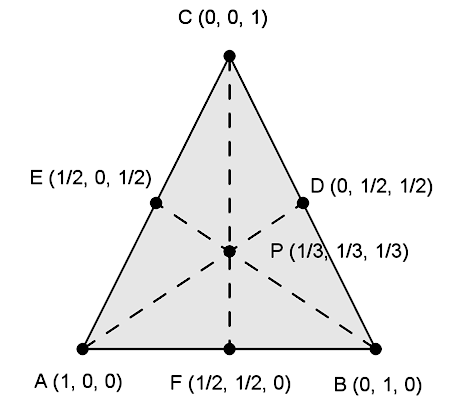
\includegraphics[scale=0.3]{Images/barycentric.png}
    \caption{Barycentric coodrinates of a 2-simplex. Here, the simplex is $s=\langle A,B,C\rangle$ and the triples of numbers next to each point $\alpha\in |s|$ in this triangle correspond to the list of values $(\alpha(A),\alpha(B),\alpha(C))$. The values of $\alpha$ thus represent the proportions in which $A,B,C$ have to be ``mixed'' to get a point inside this geometric realization of the simplex.\label{fig. simplex}}
\end{figure}


In the future we write $|K|=|K|_c$ and call this space the \emph{geometric realization} of $K$. For a simplex $s$ we define the \emph{closed simplex} $|s|\subset |K|$ as $|s|=\{\alpha\in|K|\mid \alpha(e)\neq 0\Rightarrow e\in s\}$ and the \emph{open simplex} as $\langle s\rangle=\{\alpha\in |K|\mid \alpha(e)\neq 0\Leftrightarrow e\in s\}$. The \emph{combinatorial boundary} of $|s|$ is $\partial|s|=|s|\setminus\langle s\rangle$.

\begin{defn}[Standard simplices in $\bbR^k$]
    Let $x_0,\ldots,x_n$ be affinely independent (i.e.\ $\sum_i\alpha_i x_i=0$ and $\sum_i\alpha_i=0$ imply $\alpha_j=0$). Then the simplex spanned by them is \[\langle x_0,\ldots,x_n\rangle=\left\{\sum_i \alpha_i x_i\mid \alpha_i\geq 0,\sum_i \alpha_i=1\right\}.\]
\end{defn}
\begin{defn}
    If $K=(E,S)$ is a simplicial complex and $\{x_e\mid e\in E\}$ a set of points in $\bbR^k$, and if a map
    \[f:|K|\to \bbR^k,\quad \alpha\mapsto \sum_{e\in E}\alpha(e)x_e\]
    is an embedding (say, topological), then $f(|K|)$ is called a simplicial polyhedron in $\bbR^k$ of type $K$, or a polyhedral realization of $K$ in $\bbR^k$.
\end{defn}
\begin{defn}[Triangulation]\index{Triangulation}
    Let $X$ be a topological space. A triangulation of $X$ is a triple $(X,K,f)$ where $K$ is a simplicial complex $K$ such that there is a homeomorphism $f:X\to |K|$.
\end{defn}

It is known that all differentiable manifolds can be triangulated, and the triangulation can be chosen so that on each simplex it is a smooth embedding.

\begin{defn}[Simplicial homology]\index{Homology!simplicial}
    For a simplicial complex $K=(E,S)$ define the group $C_p(K)$ of \emph{simplicial $p$-chains} as the free Abelian group generated by the set of all $p$-simplices in $K$. That is, elements of $C_p(K)$ are formal sums $\sum_{s} c_s s$, where $s$ runs over all $p$-simplices in $K$, and only a finite number of coefficients $c_s\in \bbZ$ are nonzero at once.
    
    Define the \emph{boundary operator}\index{Boundary operator}
    \[\partial:\; C_p(K)\to C_{p-1}(K),\quad \partial\langle e_0,\ldots,e_p\rangle=\sum_{i=0}^p(-1)^p\langle e_0,\ldots,\wh{e}_i,\ldots,e_p\rangle,\]
    where the hat means skipping a vertex. It is easy to check that $\partial^2=0$, therefore we have the \emph{chain complex}\index{Complex!of simplicial chains}
    \[\cdots\to C_2(K)\overset\partial\to C_1(K)\overset\partial\to C_0(K)\to 0.\]
    The group of $p$-cycles is $Z_p=\ker \restr{\partial}{C_p(M)}$ and the group of $p$-boundaries is $B_p=\restr{\im\partial}{C_{p+1}(M)}$. The \emph{simplicial homology groups} of $K$ are defined as
    \[H_p(K)=Z_p/B_p.\]
\end{defn}

Intuitively, $H_p$ detects the ``$p$-dimensional holes'' in the complex, because it consists of cycles that are not boundaries of anything $p+1$-dimensional.

\begin{defn}[Orientations on simplices and complexes]\index{Orientation!on simplicial complexes}
    An orientation on an $n$-simplex $s$ is an ordering of its elements into an $(n+1)$-tuple written as \[s=\langle e_0,\ldots,e_n\rangle.\]
    Orientations are considered to be equivalent if they differ by an even permutation of the vertices, i.e.\ we identify positively reordered tuples with each other. 
    
    In simplicial $p$-chains, sometimes the chain $-s$ is identified with $s$ oriented the opposite way.
    
    An orientation on a complex $K=(E,S)$ is a partial order on $E$ that induces an orientation on each simplex of $K$ (i.e.\ orientations of faces of a simplex can be induced from the orientation of the simplex). Orientations are considered to be equivalent if they induce equivalent orientations on all simplices.
\end{defn}

\begin{comment}
    \begin{samepage}
        \PRLsep
        \begin{center}
            {\red Lecture 21 on 10 May 2019 ended here (but Section \ref{finite dim de rham} was covered in the next lecture)}
        \end{center}
    \end{samepage}
\end{comment}

\begin{example}[Simplicial homology of $S^1$]
    A circle $S^1$ can be triangulated by a regular $n$-gon with vertices  $e_0,\ldots,e_{n-1}$ and oriented simplices $s_i=\langle e_i,e_{i+1}\rangle$, $0\leq i\leq n-1$ with the identification $e_n=e_0$. 
    Clearly 
    \[Z_0=C_0=\bbZ^n,\quad C_1=\left\{\sum_i c_i s_i \mid c_i\in \bbZ\right\}\cong \bbZ^n,\quad B_1=0.\]
    The chain complex is described by 
    \[\partial\langle e_i,e_{i+1}\rangle=\langle e_i\rangle-\langle e_{i+1}\rangle .\]
    $B_0$ consists of 0-chains $\sum c_i \langle e_i\rangle$ such that $\sum c_i=0$, thus $B_0\cong \bbZ^{n-1}$.
    Finally, $Z_1$ consists of 1-chains $\sum_i c_i s_i$ such that $c_i-c_{i+1}=0$ for all $i$, which means that $Z_1\cong \bbZ$ generated by the cycle $\sum_i s_i$. In the end, we have
    \[H_0\cong \bbZ^n/\bbZ^{n-1}\cong \bbZ,\quad H_1=Z_1\cong \bbZ. \]
    We notice that the ranks of these homology groups coincide with the dimensions of the corresponding de Rham cohomologies, see Example \ref{de Rham of circle}. We will later prove this as a general fact for all manifolds: the de Rham cohomology is isomorphic to the simplicial homology with real coefficients.
\end{example}


\begin{xca}
    If $K$ is the tetrahedron (with 2-dimensional faces included), i.e.\ a triangulation of $S^2$, compute its homology groups:
    \[H_0=\bbZ,\quad H_1=0,\quad H_2=\bbZ.\]
\end{xca}
\begin{xca}
    Triangulate the M\"obius band as in the figure.
    \begin{center}
        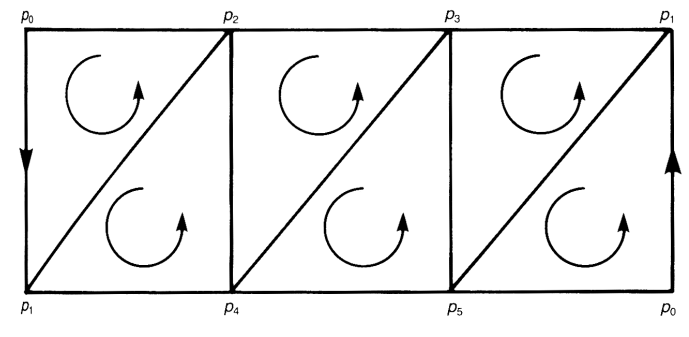
\includegraphics[scale=0.2]{Images/mobius.png}
    \end{center}
    Show that $H_2(K)=0$ and $H_1(K)=\bbZ$. In fact, the generator of $H_1$ is the loop going from the bottom left to the top right corner in the diagram above.
\end{xca}

\begin{xca}
    Triangulate the real projective plane $\bbR P^2$ (which is homeomorphic to a disk whose antipodal boundary points have been identified) as in the figure.
    \begin{center}
        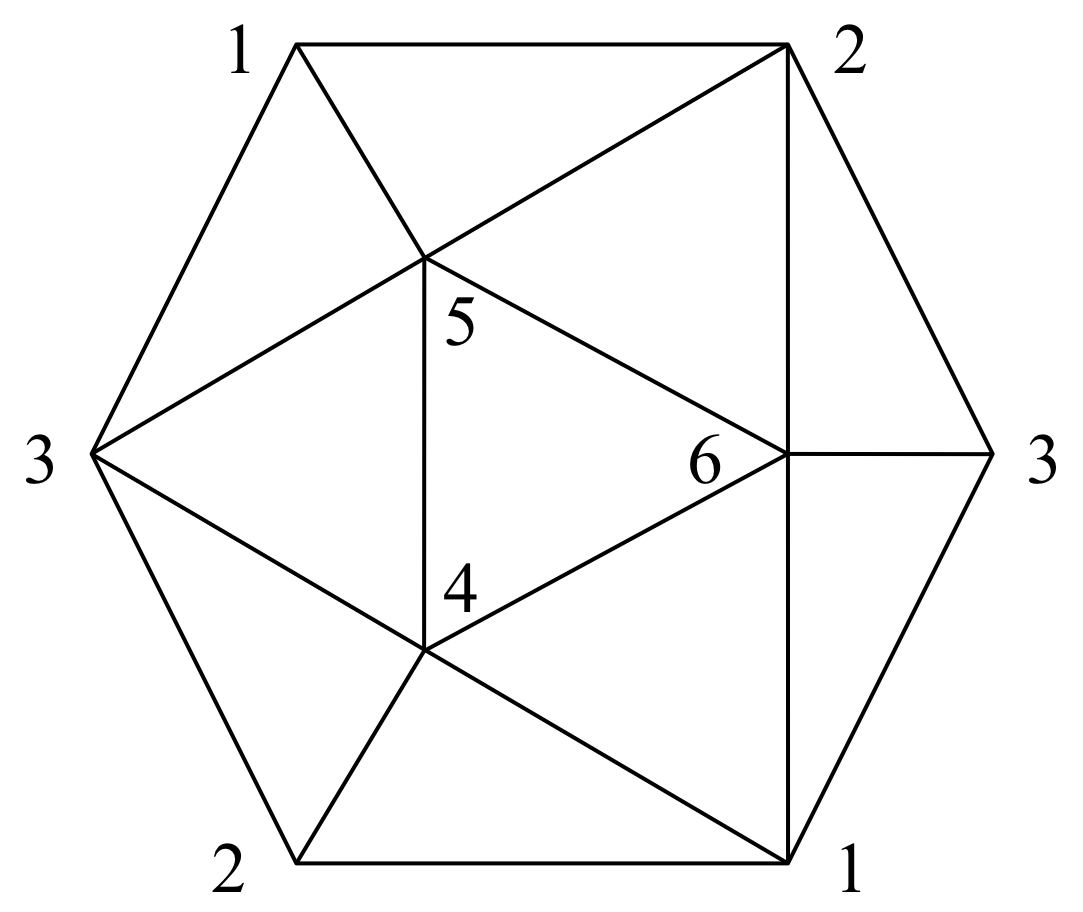
\includegraphics[scale=0.2]{Images/projectiveplane.png}
    \end{center}
    Show that $H_2(K)=0$ and $H_1(K)=\bbZ_2=\bbZ/2\bbZ$.
\end{xca}
\begin{xca}
    Triangulate the Klein bottle and show that $H_1(K)=\bbZ\oplus\bbZ_2$.
\end{xca}

\begin{defn}[Betti numbers]\index{Betti numbers}
    Let $K$ be a finite simplicial complex. By the fundamental theorem of finitely generated Abelian groups, each homology group of $K$ can be decomposed as
    \[H_p(K)=\underbrace{\bbZ^{b_p(K)}}_{\text{free part}}\oplus \underbrace{\bbZ_{m_1}\oplus \cdots \oplus \bbZ_{m_k}}_{\text{torsion part}},\]
    where $b_p(K)\geq 0$ are called \emph{Betti numbers}. 
    Since the torsion part disappears when tensor multiplied by a field containing the rationals $\bbQ$ (the tensor product is understood to be over the ring $\bbZ$ because Abelian groups are $\bbZ$-modules; then, say, $Z_m\otimes \bbQ$ consists of $a\otimes r=ma\otimes (r/m)=0$), we have
    \[H_p(K)\otimes \bbQ=\bbQ^{b_p(K)}.\]
    If $K$ is a triangulation of a smooth manifold $M$, then we will also show that $b_p(K)=\dim H_{\rm dR}^p(M)$.
\end{defn}

\begin{defn}[Euler characteristic]\index{Euler characteristic}
    If $K$ is a finite $n$-dimensional simplicial complex, then there are two definitions of the Euler characteristic $\chi(K)$:
    \begin{itemize}
        \item $\chi(K)=\sum_{p=0}^n (-1)^p n_p(K)$, where $n_p(K)$ is the number of $p$-simplices in $K$ (``combinatorial Euler characteristic'');
        \item $\chi(K)=\sum_{i=0}^n (-1)^p b_p(K)$, where $b_p(K)$ are the Betti numbers (``homological Euler characteristic'').
    \end{itemize}
\end{defn}

\begin{thm}[Euler-Poincar\'e]
    The two definitions of the Euler characteristic for finite simplicial complexes are equivalent. In particular, since the Betti numbers are homotopy invariants (because so is homology itself, which we will show later), so is the Euler characteristic.
\end{thm}
\begin{proof}
    Consider chain groups with rational coefficients (i.e.\ the free parts of the usual groups),
    \[C_p(K,\bbQ)\coloneqq C_p(K)\otimes\bbQ.\]
    Now the boundary operator $\partial_p:C_p(K,\bbQ)\to C_{p-1}(K,\bbQ)$ is a linear operator on $\bbQ$-vector spaces and by the rank-nullity theorem
    \[n_p(K)=\dim C_p(K,\bbQ)=\dim\ker\partial_p+\dim\im\partial_p.\]
    On the other hand,
    \[b_p(K)=\dim Z_p(K,\bbQ)/B_p(K,\bbQ)=\dim\ker\partial_p-\dim\im\partial_{p+1}.\]
    When taking alternating sums of these over $p$, we will get the same answer in both cases.
\end{proof}

\begin{xca}
    Compute the Euler characteristic of a finite graph consisting of several connected components each of which is a tree. Now what if there are loops but the graph is planar and we triangulate the loops and include them as 2-dimensional faces?
\end{xca}

\begin{xca}
    Compute the Euler characteristics of the simplicial complexes triangulating the circle, the sphere, and the torus. Compare the Euler characteristic of a sphere to that of a planar graph whose external ``face'' (the one containing the infinity in the plane) is also included.
\end{xca}




\subsection{Homological Algebra I: (Co)Homology of (Co)Chain Complexes}

\begin{defn}[(Co)chain complexes]\index{Complex!of chains}\index{Complex!of cochains}
    A chain complex $(\bm{C},d)$ in an Abelian category $\calC$ is a sequence  of morphisms 
    \[\cdots\to C_{n+1}\overset{d_{n+1}}\to C_n\overset{d_n}\to C_{n-1}\to\cdots\]
    indexed by $n\in \bbZ$, such that $d_n\circ d_{n+1}=0$.
    
    Similarly, a cochain complex is a sequence
    \[\cdots\to C^{n-1}\overset{d^{n-1}}\to C^n\overset{d^n}\to C^{n+1}\to\cdots\]
    such that $d^{n+1}\circ d^n=0$.
\end{defn}

Note that there is no actual difference between chain and cochain complexes, since simply changing the enumeration $n\mapsto -n$ turns one into the other. Therefore all general results need to be proven only for chain complexes.

\begin{defn}[(Co)cycles, (co)boundaries, (co)homologies of complexes]\index{Homology!of a chain complex}\index{Cohomology!of a cochain complex}
    For a chain complex $(\bm{C},d)$, $n$-cycles, $n$-boundaries, and homologies are defined as 
    \[Z_n(\bm{C},d)=\ker d_n,\quad\quad B_n(\bm{C},d)=\im d_{n+1},\quad\quad H_n(\bm{C},d)=Z_n(\bm{C},d)/B_n(\bm{C},d).\]
    
    Similarly, for a cochain complex $(C^\bullet,d)$, we have cocycles, coboundaries, and cohomologies:
    \[Z^n(C^\bullet,d)=\ker d_n,\quad\quad B^n(C^\bullet,d)=\im d^{n-1},\quad\quad H^n(C^\bullet,d)=Z^n(C^\bullet,d)/B^n(C^\bullet,d).\]
\end{defn}

\begin{defn}[Chain map]
    If $(\bm{B},\delta )$ and $(\bm{C},d)$ are two chain complexes, then a chain map $f:\bm{B}\to \bm{C}$ is a sequence of maps $f_n:B_n\to C_n$ such that $d_n\circ f_n=f_{n-1}\circ \delta_n$, i.e.\ such that the full diagram commutes:
    \[\begin{tikzcd}[every matrix/.append style={name=m},
        execute at end picture={\draw [<-] ([xshift=-8mm,yshift=-10mm]m-1-3.north) arc[start angle=-90,delta angle=-270,radius=0.2cm];
        \draw [<-] ([xshift=-8mm,yshift=-10mm]m-1-4.north) arc[start angle=-90,delta angle=-270,radius=0.2cm];}]
        \cdots\arrow[r] & B_{n+1}\arrow[r]\arrow[d,swap,"f_{n+1}"] & B_{n} \arrow[r]\arrow[d,swap,"f_n"] & B_{n-1}\arrow[d,"f_{n-1}"]\arrow[r] & \cdots \\
       \cdots\arrow[r] & C_{n+1}\arrow[r] & C_n\arrow[r] &C_{n-1} \arrow[r] &\cdots
    \end{tikzcd}\]
    Similarly one defines cochain maps between cochain complexes.
\end{defn}

\begin{prop}
    All chain complexes in an Abelian category $\calC$ with chain maps between them comprise an Abelian category called $\mathsf{Comp}(\calC)$.
\end{prop}
\begin{proof}
    By the Freyd-Mitchell theorem, we only need to prove this for $\calC=R\text{-}\mathsf{Mod}$. For such a category it is obvious what the structure of an Abelian category on complexes is: the zero object is the zero complex; direct sums are defined by summing in each degree; the kernel and cokernel of $f$ are the complexes consisting of $\ker f_n$ and $\coker f_n$; images and coimages coincide because they do so in $\calC$.
\end{proof}

\begin{defn}[Positive complexes]
    A chain complex $\bm{C}$ is called positive if $C_n=0,n<0$. All positive complexes form the full subcategory $\mathsf{Comp}_{\geq 0} (\calC)$ of $\mathsf{Comp}(\calC)$:
    \[\cdots\to C_n\to C_{n-1}\to\cdots\to \to C_1\to C_0\to 0.\]
    
    A negative chain complex
    \[0\to C_0\to C_{-1}\to \cdots \to C_{-n}\to C_{-n-1}\to\cdots\]
    is identified with a positive cochain complex 
    \[0\to C^0\to C^{1}\to \cdots \to C^{n}\to C^{n+1}\to\cdots\]
    by setting $C^n=C_{-n}$ and $d^n=d_{-n}$.
\end{defn}

\begin{prop}
    If $\calC$ is an Abelian category, then the $n$-th homology $H_n:\mathsf{Comp}(\calC)\to \calC$ is an additive (covariant) functor for all $n\in \bbZ$.
\end{prop}
\begin{proof}
    Given a chain map $f:\bm{A}t\to \bm{B}$, we need to construct a morphism $H_n(f):H_n(\bm{A})\to H_n(\bm{B})$. Since $H_n(\bm{A})=Z_n(\bm{A})/B_n(\bm{A})$, we can try to take a $z$ such that
    \[f_n:Z_n(\bm{A})\to B_n,\quad z\mapsto f_n(z)\]
    and define
    \[H_n(f):H_n(\bm{A})\to H_n(\bm{B}),\quad [z]\to \left[f_n(z)\right],\]
    where equivalence classes are taken w.r.t.\ to the quotients by $B_n(\bm{A})$ and $B_n(\bm{B})$ respectively.
    
    First we need to check that $f_n(z)\in Z_n(\bm{B})$. We will use the same symbol $d_n$ for morphisms in both complexes. By the definition of a chain map, $d_n(f_n(z))=f_{n-1}(d_n(z))=0$ since $z\in B_n(\bm{A})$.
    
    Next we need to check correctness, i.e.\ independence of $H_n(f)([z])$ of the choice of representative. Let $z,z'\in Z_n(\bm{A}):[z]=[z']\Leftrightarrow z-z'\in B_n(\bm{A})$, then
    \[\exists y\in A_{n+1}: d_{n+1}(y)=z-z'\implies d_{n+1}(f_{n+1}(y))=f_n(z)-f_n(z'),\]
    which means that $f_n(z)-f_n(z')$ is a boundary, proving what we wanted.
    
    To check functoriality, say we have two chain maps
    \[\bm{A}\overset f\to \bm{B}\overset g\to \bm{C}.\]
    We need to show the commutativity of the triangle
    \[
    \begin{tikzcd}
        H_n(\bm{A}) \arrow[rr,"H_n(f)"]\arrow[dr,swap,"H_n(g\circ f)"]&& H_n(\bm{B})\arrow[dl,"H_n(g)"]\\
        & H_n(\bm{C}) &
    \end{tikzcd}
    \]
    We have 
    \[H_n(g\circ f)([z])=\left[(g\circ f)_n(z)\right]=\left[g_n\circ f_n(z)\right]=H_n(g)\left(\left[f_n(z)\right]\right)=H_n(g)\left(H_n(f)[z]\right)=H_n(g)H_n(f)([z]).\]
    
    Finally, additivity is trivial since $f_n$ are homomorphisms:
    \[H_n(f+f')=H_n(f)+H_n(g').\]
\end{proof}

\begin{rem}
    On cochain complexes, this functor is of course contravariant.
\end{rem}

From now on we write
\[f_\ast=H_n(f),\quad\quad g^\ast=H^n(g)\]
for the descendants of maps in (co)homology.

\begin{thm}[Connecting homomorphism lemma]\label{connecting hom in homology}
    Let 
    \[0\to \bm{A}\overset i\to \bm{B}\overset\pi\to \bm{C}\to 0 \]
    be a short exact sequence of chain complexes. Then for each $n$ there is a \emph{connecting homomorphism}
    \[\delta=\delta_n:H_n(\bm{C})\to H_{n-1}(\bm{A}),\quad [z]\to \left[i_{n-1}^{-1} d_n\pi_n^{-1}(z)\right].\]
\end{thm}
\begin{proof}
    Several checks need to be done. First, why does $d_n\pi_n^{-1}(z)\in\im i_{n-1}$? Let $y:\pi_n(y)=z$, then $d_n(y)\in B_{n-1}$. Since $z\in Z_n(\bm{C})$ we have $\pi_{n-1}(d_n(y))=d_n(\pi_n(y))=d_n(z)=0$. Therefore $\exists ! x\in A_{n-1}:i_{n-1}(x)=d_n(y)$, and we have a well defined map
    \[z\mapsto x.\]
    
    Next, we need to verify that $d_{n-1}(x)=0$ and the class $[x]\in H_{n-1}(\bm{A})$ is independent of the choice of $y$.
    Moreover, one needs to check that if $[z]=[z']$, then $[x]=[x']$. Lastly, we need to check that $\delta$ is a homomorphism. These checks are left as an exercise.
\end{proof}

\begin{thm}[Zig-zag lemma/Long exact sequence in homology]\label{thm long exact seq in homology}
    For any short exact sequence of complexes 
    \[0\to \bm{A}\overset i\to \bm{B}\overset\pi\to \bm{C}\to 0 ,\]
    the induced sequence in homology
    \[\cdots \to H_{n+1}(\bm{C})\overset{\delta_{n+1}}\to H_n(\bm{A})\overset{i_\ast}\to H_n(\bm{B})\overset{\pi_\ast}\to H_n(\bm{C})\overset{\delta_n}\to H_{n-1}(\bm{A})\to \cdots \]
    is exact.
\end{thm}
\begin{proof}
    It is easy to see that for any complex $\bm{C}$ the two \emph{``fundamental sequences''}
    \[0\to Z_n(\bm{C})\to C_n\overset{d_n}\to B_{n-1}(\bm{C})\to 0,\]
    \[0\to B_n(\bm{C})\to Z_n(\bm{C})\to H_n(\bm{C})\to 0\]
    are short exact.
    This one is also obviously exact:
    \[0\to B_n(\bm{C})\to C_n\to C_n/B_n(\bm{C})\to 0.\]
    Using the exactness of the first sequence, we also have the exactness of this one:
    \[0\to H_n(\bm{C})\to C_n/B_n(\bm{C})\to \underbrace{B_{n-1}(\bm{C})}_{\cong C_n/Z_n(\bm{C})}\to 0.\]
    
    Putting it all together, we conclude the exactness of this sequence:
    \[0\to H_n(\bm{C})\to C_n/B_n(\bm{C})\to Z_{n-1}(\bm{C})\to H_{n-1}(\bm{C})\to 0.\]
    Now let us use this sequence for the columns of one large diagram:
    \[\begin{tikzcd}
        && 0\ar{d}& 0\ar{d} &0\ar{d} &&\\
        & & H_n(\bm{A}) \ar{r} \ar{d} & H_n(\bm{B})\ar{r} \ar{d} &  H_n(\bm{C}) \ar{d}   %\arrow[ddll,"\delta",rounded corners
        & & \\
        &  &  A_n/B_n(\bm{A}) \ar{r} & B_n/B_n(\bm{B}) \ar{r} \ar{dd} &  C_n/B_n(\bm{C})\ar{r}\ar{dd} & 0 &  ~\\[-10pt]
        & & &  ~ & & \ar[r, phantom, ""{coordinate, name=Y}] & ~\\[-10pt]
        ~&  \ar[l, phantom, ""{coordinate, name=Z}] 0 \ar{r} &  Z_{n-1}(\bm{A}) \ar[uu,leftarrow,crossing over]\ar{r} \ar{d} &  Z_{n-1}(\bm{B}) \ar{r} \ar{d} &  Z_{n-1}(\bm{C}) \ar{d} & &  \\
              & &  \ar[from=uuuurr, "\delta_n", dashed,crossing over, rounded corners,
                      to path=
                              { -- ([xshift=2ex]\tikztostart.east)
                              -| (Y) [near end]\tikztonodes
                              -| (Z) [near end]\tikztonodes
                              |- ([xshift=-2ex]\tikztotarget.west)
                               -- (\tikztotarget)}
                    ] H_{n-1}(\bm{A})\ar{r}\ar{d}
               &  H_{n-1}(\bm{B}) \ar{r}\ar{d}
               &  H_{n-1}(\bm{C})\ar{d}
               & 
               & \\
        && 0& 0 &0 &&\\
    \end{tikzcd}\]
    The exactness of the rows can be checked directly using the exactness of $\bm{A}\to \bm{B}\to\bm{C}$. Then this is in fact exactly the type of diagram for which we can apply the Snake Lemma \ref{snake lemma} and establish the existence of $\delta_n$. It only remains to check that the construction of $\delta_n$ in the Snake Lemma exactly coincides with the one in Proposition \ref{connecting hom in homology}.
\end{proof}
\begin{cor}
    The Snake lemma is equivalent to the Zig-zag lemma.
\end{cor}
\begin{proof}
     The proof of Theorem \ref{thm long exact seq in homology} shows that the Snake Lemma implies the long exact sequence in homology. The converse also trivially holds since we can apply the Zig-zag lemma to a short exact sequence of complexes concentrated in just two degrees of the form $0\to \ker\pi \to \im\pi \to 0$ (let the two other complexes have $\rho $ and $\sigma$ instead of $\pi$) and obtain the long exact sequence of homologies, which reads
    \[0\to \ker\pi \to \ker\rho\to \ker\sigma\to \coker\pi\to \coker\rho\to\coker\sigma\to 0, \]
    which is exactly the Snake Lemma \ref{snake lemma}.
\end{proof}

\begin{comment}
    \begin{samepage}
        \PRLsep
        \begin{center}
            {\red Lecture 22 on 17 May 2019 ended here (included Section \ref{finite dim de rham})}
        \end{center}
    \end{samepage}
\end{comment}


\begin{prop}[Naturality of the connecting homomorphism\footnote{Tape worm lemma?}]\label{naturality of connecting hom}
    Given a commutative diagram with exact rows in the category $\mathsf{Comp}(\calC)$
    \[\begin{tikzcd}
        0\arrow[r] & \bm{A}\arrow[r,"i"]\arrow[d,swap,"f"] & \bm{B} \arrow[r,"p"]\arrow[d,swap,"g"] & \bm{C}\arrow[d,"h"]\arrow[r] & 0 \\
       0\arrow[r] & \bm{A}'\arrow[r,"j"] & \bm{B}'\arrow[r,"q"] &\bm{C}' \arrow[r] &0
    \end{tikzcd}\]
    there is a commutative diagram in $\calC$ with exact rows
    \[\begin{tikzcd}
        ~\arrow[r]& H_n(\bm{A})\arrow[r,"i_\ast"]\arrow[d,"f_\ast"] & H_n(\bm{B}) \arrow[r,"p_\ast"]\arrow[d,"g_\ast"] & H_n(\bm{C})\arrow[d,"h_\ast"]\arrow[r,"\delta"] & H_{n-1}(\bm{A})\arrow[d,"f_\ast"]\arrow[r]&~ \\
       ~\arrow[r] & H_n(\bm{A}')\arrow[r,"j_\ast"] & H_n(\bm{B}')\arrow[r,"q_\ast"] &H_n(\bm{C}') \arrow[r,"\delta'"] &H_{n-1}(\bm{A}')\arrow[r]&~ 
    \end{tikzcd}\]
    In other words, morphisms between exact sequences of complexes naturally induce morphisms between the exact sequences in homology, i.e.\ the connecting homomorphism $\delta$ is natural w.r.t.\ such morphisms.
\end{prop}
\begin{proof}
     The exactness of the rows is the content of the theorem about the long exact sequence. The commutativity of the first two squares follows from the functoriality of $H_n$. Checking the commutativity of the square $\delta'\circ h_\ast=f_\ast\circ \delta$ requires expanding the first commutative diagram in $\mathsf{Comp}(\calC)$ into a 3-dimensional diagram in $\calC$.
     \[
     \begin{tikzcd}
        &
        0 
        \ar{rr}
        & &
        A_n
        \ar{dl}[swap, sloped, near start]{d}
        \ar{rr}{i}
        \ar[]{dd}[near start]{f_\ast}
        & & B_n
        \ar{dd}[near start]{g_\ast}
        \ar{rr}{p}
        \ar{dl}[swap, sloped, near start]{d}
        & & C_n
        \ar{dd}[near start]{h_\ast}
        \ar{dl}[swap, sloped, near start]{d}
        \ar{rr}
        & &
        0
        \\
        0
        \ar{rr}
        & &
        A_{n-1}
        \ar[crossing over]{rr}[near end]{i}
        & & B_{n-1}
        \ar[crossing over]{rr}[near end]{p}
        & & C_{n-1}
        \ar[crossing over]{rr}
        & &
        0
        \\
        &
        0
        \ar{rr}
        & &
        A_n'
        \ar[near start]{rr}{j}
        \ar[sloped, swap]{dl}{d}
        & & B_n'
        \ar[near start]{rr}{q}
        \ar[sloped, swap]{dl}{d}
        & & C_n'
        \ar[sloped, swap]{dl}{d}
        \ar{rr}
        & &
        0
        \\
        0
        \ar{rr}
        & &
        A_{n-1}'
        \ar{rr}{j}
        \ar[crossing over, leftarrow, near start]{uu}{f_\ast}
        & & B_{n-1}'
        \ar{rr}{q}
        \ar[crossing over, leftarrow, near start]{uu}{g_\ast}
        & & C_n'
        \ar[crossing over, leftarrow, near start]{uu}{h_\ast}
        \ar{rr}
        & &
        0
        \end{tikzcd}
     \]
     Taking $[c]\in H_n(\bm{C})$, we must show that $f_\ast\delta [c]=\delta ' h_\ast [c]$. Let $b\in B_n$ be such that $p(b)=c$. Then $\delta [c]=[a]$, where $i(a)=d(b)$. Hence $f_\ast \delta [c]=[f(a)]$. 
     
     On the other hand, since $h$ is a chain map, $q(g(b))=h(p(b))=h(c)$. Hence we can use $g(b)$ as the preimage of $h(c)$ in $B_n'$, so by construction of the connecting homomorphism, $\delta '[h(c)]=[a']$ where $j(a')=d(g(b))$. But $j(f(a))=g(i(a))=g(d(b))=d(g(b))=j(a')$ and so $f(a)=a'$ because $j$ is injective. Therefore $\delta'h_\ast [c]=[a']=[f(a)]$, which coincides with the l.h.s.\ computed above.
\end{proof}

Naturality is instrumental in many arguments involving long exact sequences because it means that we can apply sequences of chain maps to long exact sequences and preserve the commutativity of diagrams.

\begin{prop}[Algebraic Mayer-Vietoris sequence]
    If in the setting of Theorem \ref{naturality of connecting hom}, $h_\ast$ is also an isomorphism in homology, then one has the long exact sequence
    \[\cdots \to H_{n+1}(\bm{B}')\overset\Delta\to H_n(\bm{A})\overset{(f_\ast,i_\ast)}\longrightarrow H_n(\bm{A}')\oplus H_n(\bm{B})\overset{j_\ast- g_\ast}\longrightarrow H_n(\bm{B}')\overset{\Delta}\to H_{n-1}(\bm{A})\to \cdots\]
    where $\Delta=\delta \circ h_\ast^{-1}\circ q_\ast$.
\end{prop}
\begin{proof}
     Exercise.
\end{proof}

The relation of this Proposition to the \gls{mv} sequence in de Rham cohomology will become clear when we get to relative (co)homology and the excision property. The isomorphism $h_\ast$ in question is $H_n(U,U\cap V)\cong H_n(M,V)$ for $M=U\cup V$. A rough visualization of $H_n(X,Y)$ with $Y\subset X$ is the homology of the space obtained from $X$ by contracting $Y$ into one point. Then it is clear that contracting $V$ inside $M$ has the ``same'' result as contracting $U\cap V$ inside $U$. 


\begin{defn}[Maps of degree $p$]
    Let $\bm{C}$ and $\bm{D}$ be two chain complexes in $\calC$. A map of degree $p$ between them, denoted $s:\bm{C}\to \bm{D}$, is a collection of maps $s_n:C_n\to D_{n+p}$. Note that no commutativity is required here!
\end{defn}


Now that we know that $H_n$ is a functor, it is natural to ask how much $H_n(f)$ actually depends on $f$. It turns out that $H_n(f)$ is invariant under homotopies of $f$ defined in the following categorical sense.


\begin{defn}
    Let $f,g:\bm{B}\to \bm{C}$ be two chain maps. They are called homotopic ($f\sim g$) if there is a map of degree $+1$ denoted $s:\bm{B}\to \bm{C}$ such that 
    \[\forall n,\quad f_n-g_n=d_{n+1}s_n+s_{n-1}d_n.\]
    (As usual, we use $d_n$ to denote the differentials in all complexes at once).
    This can be visualized by the following \emph{non-commutative} diagram:
     \[\begin{tikzcd}
        \cdots\ar[r] & B_{n+1}\ar[r]\ar[dd,swap, xshift=-.75ex,"f_{n+1}"]\ar[dd,xshift=.75ex,"g_{n+1}"] & B_{n} \arrow[r]\ar[dd,swap,xshift=-.75ex,"f_n"]\ar[dd,xshift=.75ex,"g_n"]\ar[ddl,swap,sloped, near start,"s_n"] & B_{n-1}\ar[dd,swap,xshift=-.75ex,"f_{n-1}"]\ar[dd,xshift=.75ex,"g_{n-1}"]\ar[r]\ar[ddl,swap, near start,sloped,"s_{n-1}"] & \cdots \\
        &&&&\\
       \cdots\ar[r] & C_{n+1}\ar[r] & C_n\ar[r] &C_{n-1} \ar[r] &\cdots
    \end{tikzcd}\]
\end{defn}

\begin{thm}
    Homotopic chain maps induce the same morphism in homology.
\end{thm}
\begin{proof}
     Let $s:\bm{B}\to\bm{C}$ be the homotopy. If $z$ is an $n$-cycle, dropping subscripts, $d z=0$, then
     \[f(z)-g(z)=d(s(z))+s(d(z))=d(s(z)),\]
     i.e.\ $f(z)-g(z)\in B_n(\bm{C})$ and $f_\ast=g_\ast$.
\end{proof}

\begin{defn}[Acyclic, contractible complexes]\index{Acyclic complex}\index{Contractible complex}
    A complex is called acyclic if all its (co)homologies are trivial. A complex $\bm{C}$ is called contractible if there exists a homotopy $1_{\bm{C}}\sim 0_{\bm{C}}$. 
    All contractible complexes are acyclic since contractibility implies $1_{H_n(\bm{C})}=0_{H_n(\bm{C})}$.
\end{defn}

\begin{defn}[Quasi-isomorphisms]\index{Quasi-isomorphism}
    Two complexes $\bm{A},\bm{B}$ are called quasi-isomorphic (or \emph{weakly equivalent}) if there is a chain map $f:\bm{A}\to \bm{B}$ such that $f_\ast=H_n(f):H_n(\bm{A})\to H_n(\bm{B})$ is an isomorphism for all $n$.
\end{defn}

\begin{defn}[Homotopy equivalence]\index{Homotopy equivalence}
    Two complexes $\bm{A},\bm{B}$ are called homotopy equivalent if there are two chain maps $f:\bm{A}\to \bm{B}$ and $g:\bm{B}\to\bm{A}$ such that
    \[f\circ g\sim 1_{\bm{B}},\quad g\circ f\sim 1_{\bm{A}}.\]
    Clearly homotopy equivalent complexes are quasi-isomorphic.
\end{defn}


\begin{xca}\label{Lie derivative homotopy operator}
    Check that a Lie derivative $\Lie_X$ is a cochain map on the de Rham complex. Furthermore, show that applying a Lie derivative $\Lie_X$ to a differential form doesn't change its class in de Rham cohomology. For this, find the homotopy operator between $\Lie_X$ and the zero morphism.
\end{xca}


\subsection{Singular Homology}

de Rham cohomology is defined only for smooth manifolds, and simplicial homology is defined only for triangulable spaces. The type of homology we define now works for all topological spaces, but proving its properties for nicer spaces (like manifolds) requires extra work. 

\begin{defn}[Singular simplices]\index{Simplex!singular}
    We denote by $\Delta^n$ the standard $n$-simplex $\Delta^n=\{\sum_{i=0}^{n} \alpha_i e_i\mid \sum_i\alpha_i=1\}$, where $\{e_i\}_{i=0}^{n}$ is the standard basis in $\bbR^{n+1}$. Let $X$ be a topological space. A singular $n$-simplex in $X$ is a continuous map $\sigma\in C(\Delta^n, X)$ (no other constraints, hence ``singular''). The group $C_n(X)$ of singular $n$-chains is the free Abelian group generated by the set $C(\Delta^n,X)$. Sometimes we will write $C^{\text{sing}}_n(X)$ to distinguish from other kinds of chain groups.
\end{defn}
\begin{defn}[Singular homology]\index{Homology!singular}
    The boundary map $\partial_n:C_n(X)\to C_{n-1}(X)$ is defined as before:
    \[\partial_n\sigma=\sum_i (-1)^i\restr{\sigma}{\langle e_0,\ldots,\wh{e}_i,\ldots,e_n\rangle},\]
    where we implicitly identify the faces of $\Delta^n$ with $\Delta^{n-1}$ while preserving the order of vertices, so that $\restr{\sigma}{\langle e_0,\ldots,\wh{e}_i,\ldots,e_n\rangle}$ is a singular $(n-1)$-simplex.
    
    Singular homology groups are defined as
    \[H_n(X)=\ker\partial_n/\im\partial_{n+1}.\]
\end{defn}

Unlike with simplicial homology, here it is immediately obvious that homeomorphic spaces have isomorphic singular homologies. The price we pay for this is that the rank of $C^{\text{sing}}_n(X)$ is uncountably large, so it is not clear at a glance whether singular homologies of spaces that have finitely generated simplicial homologies are also finitely generated. 

\begin{prop}
    If $X$ consists of $l$ path-connected components, then $H_0(X)\cong \bbZ^l$.
\end{prop}
\begin{proof}
     It suffices to prove this for $l=1$, i.e.\ a path-connected $X$. We have $H_0(X)=C_0(X)/\im\partial_1$. A singular 0-chain in $X$ is just a finite sum $\sum_i n_i p_i$ where $p_i$ are points in $X$ and $n_i\in\bbZ$. Define the homomorphism $\epsilon:C_0(X)\to \bbZ$, called the \emph{augmentation map}\index{Augmentation map}, by
     \[\epsilon\left(\sum_i n_i p_i\right)=\sum_i n_i.\]
     It is surjective as long as $X\neq\varnothing$. The claim is that $\ker\epsilon\cong\im\partial_1$ if $X$ is path-connected, so $\epsilon $ induces an isomorphism $H_0(X)\cong \bbZ$.
     
     First, it is clear by definition of $\partial$ that $\im\partial_1\subset\ker\epsilon$. For the reverse inclusion, suppose $\epsilon(\sum_i n_i p_i)=0$. Choose a path $\gamma_i$ connecting a base point $x_0$ to $p_i$. We can view $\gamma_i$ as a singular 1-simplex and have $\partial\gamma_i=p_i-x_0$. Hence $\partial(\sum_i n_i\gamma_i)=\sum_i n_i p_i$ since $\sum_i n_i=0$. Therefore $\sum n_i p_i$ is a boundary, which shows $\ker\epsilon\subset\im\partial_1$.
\end{proof}

\begin{prop}
    If $X=\text{point}$, then $H_n(X)=0$ for $n>0$ and $H_0(X)\cong \bbZ$.
\end{prop}
\begin{proof}
     In this case there is a unique singular $n$-simplex $\sigma_n$ for each $n$ and 
     \[\partial\sigma_n=\sum_{i=0}^n(-1)^i\sigma_{n-1}=\begin{cases}
     0,& n\text{ odd},\\
     \sigma_{n-1},& n\text{ even}.
     \end{cases}\]
     This the singular chain complex reads
     \[\cdots\to \bbZ\overset\cong\to \bbZ\overset 0\to \bbZ\overset\cong\to\bbZ\overset 0\to\bbZ\to 0.\]
     The homology of this complex is trivial except for $H_0\cong \bbZ $.
\end{proof}

Sometimes it is very helpful to work with a slightly modified homology that vanishes entirely for a point. The following definition achieves this.

\begin{defn}[Reduced homology]\index{Homology!reduced}
    The reduced homology groups $\wt{H}_n(X)$ are the homology groups of the \emph{augmented chain complex}
    \[\cdots C_1(X)\overset{\partial_1}\to C_0(X)\overset{\epsilon}\to \bbZ\to 0.\]
\end{defn}

The reduced homology of a point is trivial in all degrees. Also $H_n(X)\cong \wt{H}_n(X)$ for all $n>0$ and $H_0(X)=\wt{H}_0(X)\oplus \bbZ$ since $\epsilon$ induces a map $H_0(X)\to \bbZ$ with kernel $\wt{H}_0(X)$.




\subsection{Homotopy Property}

Here we show that singular homology is homotopy invariant.

\begin{wrapfigure}[10]{r}{0.2\textwidth}
    \begin{center}
        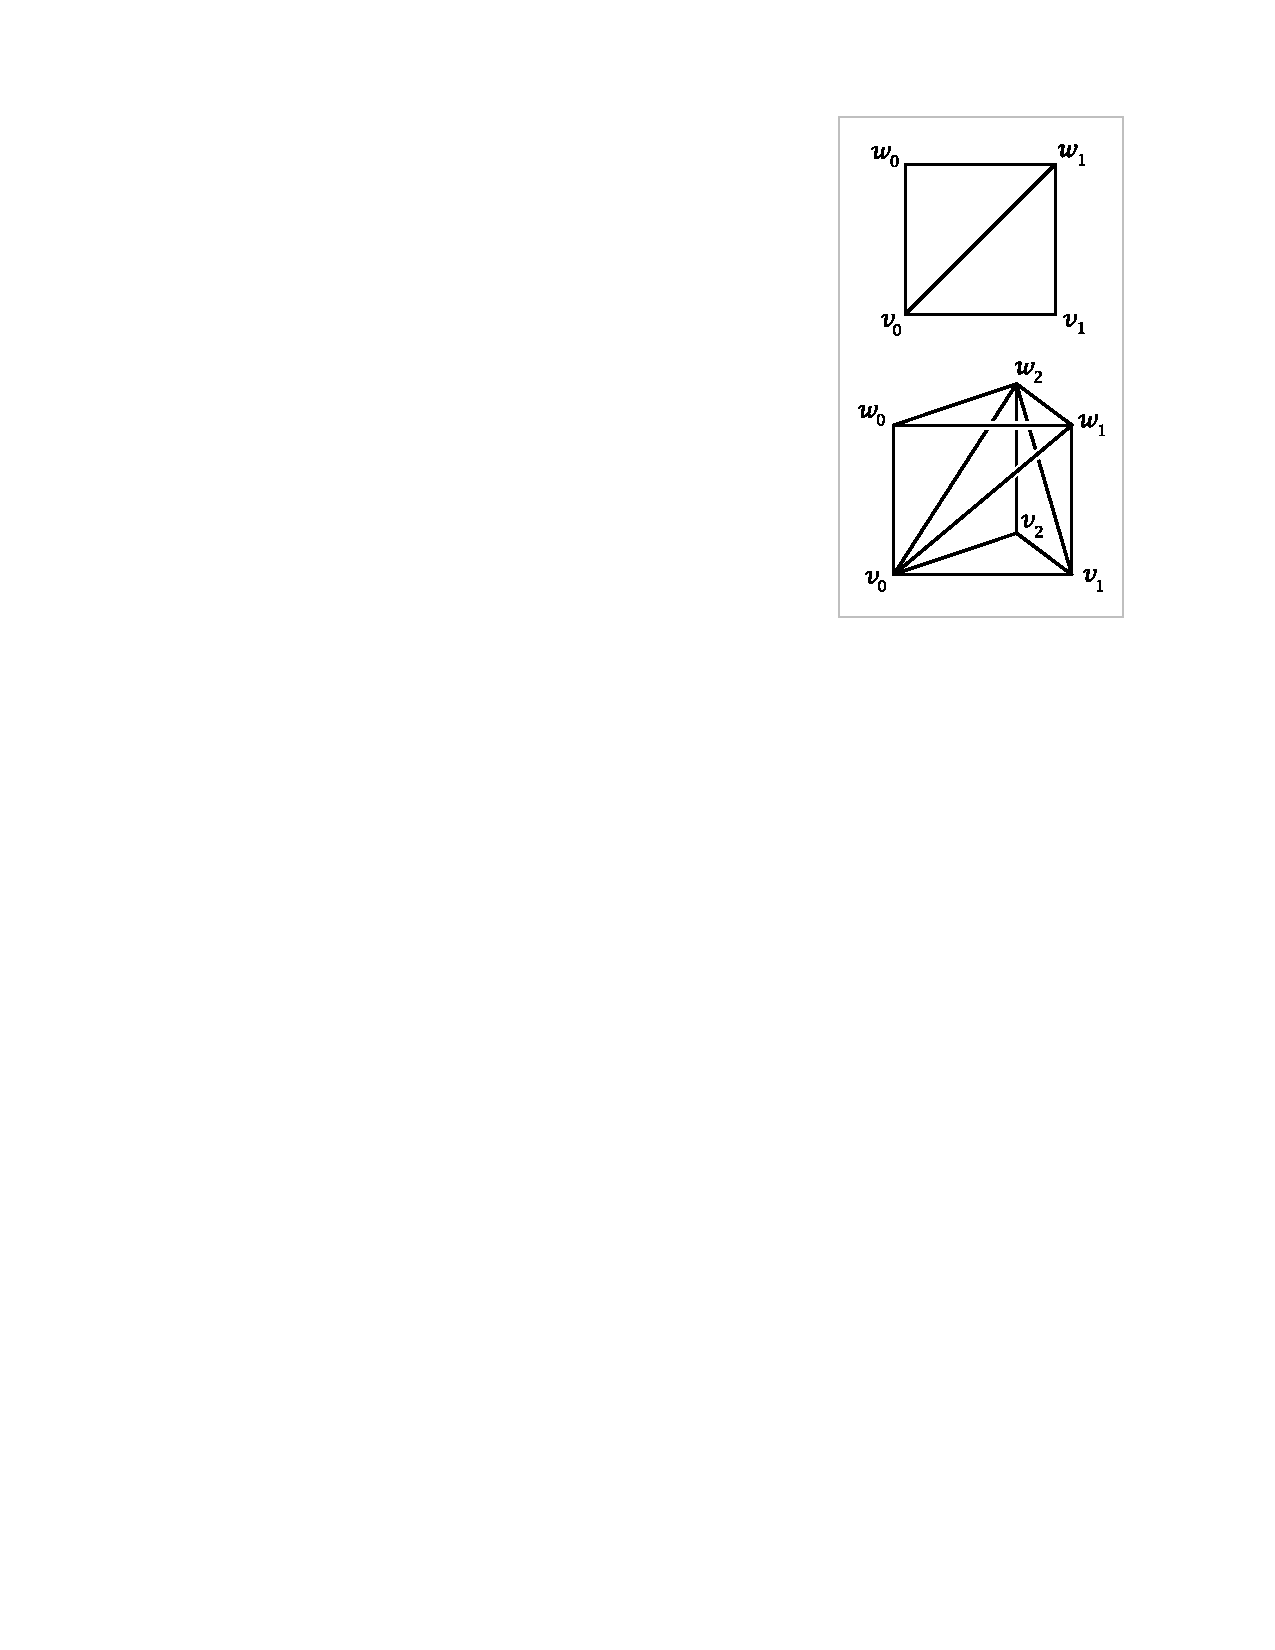
\includegraphics[width=0.2\textwidth]{Images/prism.pdf}
    \end{center}
    \caption{Triangulation of a prism.\label{Prism fig}}
\end{wrapfigure}

\begin{prop}
    If two maps $f,g\in C(X,Y)$ between topological spaces $X,Y$ are homotopic, then they induce the same homomorphism in homology
    \[f_\ast=g_\ast :H_n(X)\to H_n(Y)\]
    for all $n$. In particular, homotopy equivalent spaces have isomorphic homology groups.
\end{prop}

\begin{proof}
     The key is learning to subdivide the prism $\Delta^n\times I$ (where $I=[0,1]$) into simplices. If $\langle v_0,\ldots,v_n\rangle$ is the copy of $\Delta^n$ at the bottom of the prism and $\langle w_0,\ldots,w_n\rangle$ is the one at the top, then it is easy to check that the prism is triangulated by the $(n+1)$-simplices $\langle v_0,\ldots,v_i,w_i,\ldots,w_n\rangle$, each intersecting the next in an $n$-simplex face. The cases $n=1,2$ are shown in figure \ref{Prism fig}.
     
     Given a homotopy $F:X\times I\to Y$ from $f$ to $g$ and a singular simplex $\sigma:\Delta^n\to X$, we form the composition $F\circ(\sigma\times \id):\Delta^n\times I\to X\times I\to Y$. Using this, we define the \emph{prism operators}
     \[P:C_n(X)\to C_{n+1}(Y),\quad P(\sigma)=\sum_i(-1)^i F\circ (\sigma\times\id)\langle x_0,\ldots,v_i,w_i,\ldots,w_n\rangle.\]
     We claim that $P$ is a homotopy operator between these two chain complexes, namely
     \[g_\ast-f_\ast=\partial P+P\partial.\]
     The geometric meaning of $\partial P=g_\ast-f_\ast-P\partial$ is that the boundary of the prism equals its top $\Delta^n\times\{1\}$, minus its bottom $\Delta^n\times\{0\}$, and plus the sides $\partial\Delta^n\times I$ (compare this with Cartan's magic formula and its cohomological meaning, which is nothing but a dual to this geometric statement, see Exercise \ref{Lie derivative homotopy operator}).
     
     The proof of this identity follows easily by direct expansion and definition of the homotopy $F$ and $g\circ\sigma=g_\ast(\sigma)$ (see \cite[Thm.~2.10]{Hatcher} for more details).
\end{proof}
\begin{cor}
    If $X$ is contractible, then $\wt{H}_n(X)=0$ for any $n$.
\end{cor}


Continuous maps induce homomorphisms in reduced homology as well since the augmentation map $\epsilon$ commutes with $f_\ast$. Then the same theorem holds for reduced homologies with the same proof.




\subsection{Relative Homology and the Excision Property}

Relative homology generalizes the idea behind the \gls{mv} sequence in de Rham cohomology. Given a subset $A\subset X$ in a topological space, we ask how similar the groups $H_n(X/A)$ and $H_n(X)/H_n(A)$ are. The difference, in a sense, is measured by the relative homology.

\begin{defn}
    Let $X$ be a topological space and $A\subset X$ a topological subspace (i.e.\ a subset with the induced subset topology). The group of singular chains $C_n(A)$ can be treated as a subgroup of $C_n(X)$. Define the relative singular chain groups as $C_n(X,A)=C_n(X)/C_n(A)$. The boundary operator $\partial$ descends to these groups because $\partial(C_n(A))\subset C_{n-1}(A)$. The homology of the resulting chain complex is called the relative homology of the pair $(X,A)$.
\end{defn}

Relative homology is a covariant functor on the category of topological pairs, $H_n:\mathsf{TopPair}\to \mathsf{Ab}$.

\begin{prop}[Exact sequence of a pair]\label{exact seq of a pair}
    The exact sequence of relative chain groups
    \[0\to C_\bullet(A)\to C_\bullet (X)\to C_\bullet(X,A)\to 0 \]
    induces a long exact sequence in relative homology
    \[\cdots \to H_n(A)\to H_n(X)\to H_n(X,A)\to H_{n-1}(A)\to H_{n-1}(X)\to H_{n-1}(X,A)\to \cdots\]
\end{prop}
\begin{proof}
     The first exact sequence is the definition of relative homology and the second one is an application of the Zig-zag lemma.
\end{proof}

The same sequence exists in reduced homology. This exact sequence has a natural geometric interpretation: elements of $H_n(X,A)$ can be thought of as $n$-chains in $X$ that differ from an actual cycle in $X$ only by a chain in $A$, and the connecting homomorphism maps such a cycle into an $(n-1)$-cycle in $A$ by simply computing the boundary.

\begin{cor}
    \begin{enumerate}
        \item $H_n(X,
        \{x_0\})\cong\wt{H}_n(X)$ for all $n$.
        \item If $A$ is contractible, then $H_n(X,A)\cong \wt{H}_n(X)$ for all $n$;
        \item if $X$ is contractible, then $H_{n+1}(X,A)\cong \wt{H}_n(A)$ for all $n$.
    \end{enumerate}
\end{cor}

\begin{example}[Homology of a bouquet of circles]
    Consider $X=\bbR$ and $A\subset \bbR$ a finite subset of size $(k+1)$. Then $X/A$ is homotopy equivalent to a wedge sum of $k$ circles (a.k.a.\ a bouquet of circles). We will later show that $H_1(X,A)\cong \wt{H}_1(X/A)= H_1(X/A)$, so we have $H_1(\bigvee_{i=1}^{k}S^1)=\wt{H}_0(A)=\bbZ^{k}$. We also see that all higher homologies of the bouquet vanish. Another way to obtain this result will be from the Hurewicz theorem.
\end{example}



\begin{prop}[Exact sequence of a triple]\label{exact sequence of a triple}
    For a triple $(X,A,B)$ where $B\subset A\subset X$, the exact sequence of relative chain complexes
    \[0\to C_\bullet(A,B)\to C_\bullet (X,B)\to C_\bullet(X,A)\to 0 \]
    induces a long exact sequence in relative homology
    \[\cdots \to H_n(A,B)\to H_n(X,B)\to H_n(X,A)\to H_{n-1}(A,B)\to H_{n-1}(X,B)\to H_{n-1}(X,A)\to \cdots\]
\end{prop}
\begin{proof}
     Exercise.
\end{proof}


\begin{prop}[Homotopy property for relative homology]
    If two maps $f,g:(X,A)\to (Y,B)$ in the category of topological pairs are homotopic also through maps of pairs, then they induce the same homomorphism $f_\ast=g_\ast:H_n(X,A)\to H_n(Y,B)$.
\end{prop}
\begin{proof}
     The prism operator constructed in the proof of the homotopy property induces a relative prism operator $P:C_n(X,A)\to C_{n+1}(Y,B)$. Since we are passing to quotient groups, the formula $\partial P+P\partial=g_\ast-f_\ast$ still holds and $f_\ast,g_\ast$ are chain homotopic on relative chain groups. 
\end{proof}


For a space $X$, let $\calU=\{U_\alpha\}_\alpha$ be a collection of subspaces of $X$ whose interiors cover $X$ and let $C_n^\calU(X)$ be the subgroup of $C_n(X)$ generated by simplices whose images lie inside one of the sets in the cover. The boundary operator $\partial$ maps $C^\calU_n(X)$ to $C^\calU_{n-1}(X)$ and therefore we have a chain complex $C_\bullet^\calU(X)$ with homology groups denoted $H^\calU_n(X)$.

\begin{prop}
    With the notation just described, the inclusion $i:C_n^\calU(X)\hookrightarrow C_n(X)$ is a chain homotopy equivalence and hence induces isomorphisms
    \[H_n^\calU(X)\cong H_n(X)\]
    for all $n$.
\end{prop}
\begin{proof}
     The proof is fairly tedious with multiple technical steps and we refer the reader to \cite[Thm. 2.21]{Hatcher} for all the details. The idea is to perform iterated barycentric subdivision of all simplices to construct a quasi-inverse (chain homotopy inverse) to $i$. 
     
     \begin{enumerate}
         \item \emph{Barycenric subdivision of simplices.} Denote the barycenter of an $n$-simplex $\sigma=\langle v_0,\ldots,v_n\rangle$ by  $b=\sum_i v_i/(n+1)$. The barycentric subdivision consists of $n$-simplices $\langle b,w_0,\ldots,w_{n-1}
         \rangle$ where iteratively $\langle w_0,\ldots,w_{n-1}\rangle$ is an $(n-1)$-simplex in the barycentric subdivision of a face $\langle v_0,\ldots,\wh{v}_i,\ldots,v_n\rangle$.
         
         To us it is important that the diameter of any simplex in the barycentric subdivision of $\sigma$ is bounded by $\frac{n}{n+1}\cdot \text{diam}(\sigma)$. Since $\frac{n}{n+1}<1$, iterating the subdivision creates simplices uniformly and arbitrarily small in size.
         
         \item \emph{Barycenric subdivision of linear chains.} For a convex set $Y$ in a Euclidean space, all linear maps $\Delta^n\to Y$ generate a subgroup of $C_n(Y)$ that we denote by $L_n(Y)$, the linear chains. They form a chain complex with the same boundary operator. Each such linear simplex can be identified with a regular simplex in $Y$ itself.  For convenience we augment the complex with $L_{-1}(Y)=\bbZ$ generated by the empty simplex $\langle \varnothing \rangle$ with $\partial \sigma=\langle \varnothing \rangle$ for all $\sigma\in L_1(Y)$.
         
         Each point $b\in Y$ determines a homomorphism $b:L_n(Y)\to L_{n+1}(Y)$ defined on simplices by $b(\langle w_0,\ldots,w_n\rangle)=\langle b,w_0,\ldots,w_n\rangle$ (a ``cone operator''). It is easy to check that $\partial b+b\partial =\id$, so $b$ is a chain homotopy between the identity and zero on the augmented chain complex $L_\bullet(Y)$.
         
         Define the subdivision homomorphism $S:L_n(Y)\to L_n(Y)$ by induction in the degree. Denoting by $b_\lambda$ the image of the barycenter in a linear singular simplex $\lambda:\Delta^n\to Y$. Then the inductive formula for $S$ is $S(\lambda)=b_\lambda(S\partial\lambda)$, where $b_\lambda$ was defined above.
         
         Then one checks that $\partial S=S\partial$ so that $S$ provides a chain map from $L_\bullet(Y)$ to itself. Next we build a chain homotopy $T:L_n(Y)\to L_{n+1}(Y)$ between $S$ and the identity. It is defined inductively by $T_{n=-1}=0$ and $T(\lambda)=b_\lambda(\lambda-T\partial\lambda)$ for $n\geq 0$. The geometric interpretation of this formula is that we inductively subdivide $\Delta^n\times I$ by joining all simplices in the bottom and side faces of the prism to the barycenter of the top face, and $T$ takes the image of this subdivision under the projection $\Delta^n\times I\to \Delta^n$. Finally one verifies that $\partial T+T\partial=\id-S$.
         
         \item \emph{Barycentric subdivision of general chains.} Define $S:C_n(X)\to C_n(X)$ by setting $S\sigma=\sigma_\ast S(\Delta^n)$. It follows easily that it is a chain map, $\partial S=S\partial$. Then in a similar fashion we define $T:C_n(X)\to C_{n+1}(X)$ by $T(\sigma)=\sigma_\ast T(\Delta^n)$, and we also have $\partial T+T\partial =\id -S$.
         
         \item \emph{Iterated barycentric subdivision.} We can construct a chain homotopy between $\id$ and the iterated subdivision $S^m$, given by $D_m=\sum _{0\leq i<m}TS^i$ (easy check that $\partial D_m+D_m\partial=\id -S^m$). 
         
         For any given simplex $\sigma$ there exists a number $m(\sigma)$ such that $S^{m(\sigma)}(\sigma)$ lies in $C^\calU_n(X)$ (because the diameter of the simplices in $S^m(\Delta^n)$ will be less than the strictly positive Lebesgue number of the cover of the compact metric space $\Delta^n$ by the open sets $\sigma^{-1}(\Int U_\alpha)$ for large $m$, and by definition a set of diameter less than the Lebesgue number is contained in one of the sets in the cover). Now we define $D:C_n(X)\to C_{n+1}(X)$ by  $D(\sigma)=D_{m(\sigma)}(\sigma)$. For this operator we need to find a chain map $\rho:C_n(X)\to C_n(X)$ such that $\partial D+D\partial=\id-\rho$. This formula itself hints that $\rho(\sigma)=S^{m(\sigma)}(\sigma)+D_{m(\sigma)}(\partial\sigma)-D(\partial\sigma)$ does the job. Viewing $\rho$ as a map $C_n(X)\to C_n^\calU(X)$, we have $\partial D+D\partial=\id-i\circ\rho$. We also know $\rho\circ i=\id$ since $D$ is identically zero and $m(\sigma)=0$ on $C_n^\calU(X)$. Therefore $\rho$ is a chain homotopy inverse for $i$.
     \end{enumerate}
\end{proof}

\begin{thm}[Excision]\index{Excision}
    Given subspaces $Z\subset A\subset X$ such that $\wb{Z}\subset \Int A$, the inclusion $(X\setminus Z,A\setminus Z)\hookrightarrow (X,A)$ induces isomorphisms 
    \[H_n(X\setminus Z,A\setminus Z)\cong H_n(X,A)\]
    for all $n$. Equivalently, for subspaces $A,B\subset X$ that cover $X$, the inclusion $(B,A\cap B)\hookrightarrow (X,A)$ induces isomorphisms
    \[H_n(B,A\cap B)\cong H_n(X,A)\]
    for all $n$ (by setting $B=X\setminus Z$, $Z=X\setminus B$, in which case $A\cap B=A\setminus Z$ and the condition $\wb{Z}\subset \Int A$ is equivalent to $X=\Int A\cup\Int B$ since $X-\Int B=\wb{Z}$).
\end{thm}
\begin{proof}
     We prove the version with $X=A\cup B$. For the cover $\calU=\{A,B\}$ we have the chain groups $C_n^\calU(X)$ consisting of sums of chains in $A$ and chains in $B$. At the end of the preceding proof we established $\partial D+D\partial=\id-i\circ\rho$ and $\rho\circ i=\id$. All maps here take chains in $A$ to chains in $A$, so they induce  quotient maps when we factor out chains in $A$. These quotient maps automatically satisfy the same formulas, so the inclusion $C^\calU_n(X)/C_n(A)\hookrightarrow C_n(X)/C_n(A)$ induces an isomorphism on homology. The map $C_n(B)/C_n(A\cap B)\to C_n^\calU(X)/C_n(A)$ induced by the inclusion is obviously an isomorphism since both quotient groups are free generated by the singular $n$-simplices in $B$ that do not lie in $A$. Hence we obtain the desired isomorphism $H_n(B,A\cap B)\cong H_n(X,A)$, induced by inclusion.
\end{proof}


\begin{comment}
    \begin{samepage}
        \PRLsep
        \begin{center}
            {\red Lecture 23 on 24 May 2019 ended here}
        \end{center}
    \end{samepage}
\end{comment}


\begin{defn}[Good pair]\index{Good pair}
    $(X,A)$ is called a good pair if $A$ is a deformation retract of an open subset in $X$. That is, there is an open set $U$ such that $A\subset U\subset X$ and a map $F\in C(U\times[0,1],X)$ such that $F(x,0)=x$, $F(x,1)\in A$ for all $x\in U$ and also $F(x,t)=x$ for all $x\in A$ and $t\in [0,1]$.
\end{defn}

\begin{prop}
    For good pairs $(X,A)$ the quotient map $q:(X,A)\to (X/A,A/A)$ induces isomorphisms \[H_n(X,A)\overset{q_\ast}\cong H_n(X/A,A/A)\cong \wt{H}_n(X/A)\]
     for all $n$.
\end{prop}
\begin{proof}
     Let $U$ be a neighborhood of $A$ in $X$ that deformation retracts onto $A$. We have the commutative diagram (the commutativity is easy to check)
      \[\begin{tikzcd}
        H_n(X,A) \arrow[r,"h"]\arrow[d,"q_\ast"] & H_n(X,U)\arrow[d,"q_\ast"]\ar[r,leftarrow,"p"] & H_n(X\setminus A,U\setminus A)\arrow[d,"q_\ast"] \\
        H_n(X/ A,A/A)\arrow[r,"r"] &H_n(X/A,U/A) \ar[r,leftarrow,"k"] &H_n((X/A)\setminus (A/A),(U/A)\setminus(A/A))
    \end{tikzcd}\]
    Here $h$ is an isomorphism since in the long exact sequence of the triple $(X,U,A)$ (Proposition \ref{exact sequence of a triple}) the groups $H_n(U,A)$ are zero for all $n$ because the deformation retraction gives a homotopy equivalence of pairs $(U,A)\simeq (A,A)$ and $H_n(A,A)=0$. The same retraction induces a deformation retraction of $U/A$ onto $A/A$, so the same argument shows that $r$ is an isomorphism as well. The maps $p,k$ are isomorphisms directly by excision. The rightmost map $q_\ast$ is an isomorphism since $q$ restricts to a homeomorphism on $X\setminus A$. From the commutativity of the diagram, the leftmost $q_\ast$ is also an isomorphism.
\end{proof}

\begin{thm}
    If $(X,A)$ is a good pair, then there is an exact sequence
    \[\cdots \wt{H}_n(A)\overset{i_\ast}\to \wt{H}_n(X)\overset{\pi_\ast}\to \wt{H}_n(X/A)\overset\partial\to \wt{H}_{n-1}(A)\to \wt{H}_{n-1}(X)\to \cdots \to \wt{H}_0(X/A)\to 0,\]
    where $i:A\hookrightarrow X$ is the inclusion and $\pi:X\to X/A$ is the quotient map.
\end{thm}
\begin{proof}
     Simply combine the exact sequence of a pair (Proposition \ref{exact seq of a pair}) with the preceding proposition.
\end{proof}

\begin{cor}\label{reduced homology of spheres}
    $\wt{H}_m(S^n)=\wt{H}_{m-1}(S^{n-1})$ and by induction the only nonzero reduced homology of a sphere is $\wt{H}_n(S^n)\cong \bbZ$.
\end{cor}
\begin{proof}
     For $n>0$, take $(X,A)=(D^n,S^{n-1})$ where $D^n$ is the $n$-dimensional disk (ball). Then $X/A=S^n$. The terms $\wt{H}_i(X)=0$ since $D^n$ is contractible. Exactness implies the necessary isomorphism.
\end{proof}
\begin{cor}[Brouwer's fixed point theorem]\index{Brouwer's fixed point theorem}
    $\partial D^n$ is not a retract of $D^n$ (i.e.\ no continuous map $D^n\to \partial D^n$ that restricts to identity on the boundary). Hence every map $f:D^n\to D^n$ has a fixed point.
\end{cor}
\begin{proof}
     If $r:D^n\to \partial D^n$ is a retraction, then $r\circ i=\id$ for $i:\partial D^n\hookrightarrow D^n$ the inclusion map. The composition $\wt{H}_{n-1}(\partial D^n)\overset{i_\ast}\to \wt{H}_{n-1}(D^n)\overset{r_\ast}\to \wt{H}_{n-1}(\partial D^n)$ is then the identity on $\wt{H}_{n-1}(\partial D^n)\cong \bbZ$. But $i_\ast$ and $r_\ast$ are both zero since $\wt{H}_{n-1}(D^n)=0$, which leads to a contradiction.
     
     An existence of a map $f:D^n\to D^n$ with no fixed points would let us construct a retraction by draiwing the straight ray from $f(x)$ to $x$ for all $x$ in the ball and picking its intersection with the boundary as the image of $x$ (this acts as the identity on the boundary).
\end{proof}



\begin{cor}
    For a wedge sum of pointed spaces $\bigvee_{\alpha}X_\alpha$, the inclusions $i_\alpha:X_\alpha\hookrightarrow \bigvee_{\alpha}X_\alpha$ induce an isomorphism 
    \[\bigoplus_\alpha i_{\alpha\ast}:\bigoplus_\alpha\wt{H}_n(X_\alpha)\to \wt{H}_n\left(\bigvee_{\alpha}X_\alpha\right),\]
    provided that the base points $x_\alpha\in X_\alpha$ are such that the pairs $(X_\alpha,\{x_\alpha\})$ are good.
\end{cor}
\begin{proof}
     Reduced homology is the same as homology relative to a base point, so the result follows from the long exact sequence for $(X,A)=\left(\bigsqcup_\alpha X_\alpha, \bigsqcup_\alpha \{x_\alpha\}\right)$.
\end{proof}

\begin{cor}[Invariance of dimension]
    If nonempty open sets $U\subset \bbR^m$ and $V\subset \bbR^n$ are homeomorphic, then $m=n$.
\end{cor}
\begin{proof}
     For $x\in U$, we have $H_k(U,U\setminus \{x\})\cong H_k(\bbR^m,\bbR^m\setminus \{x\})$ by excision. From the long exact sequence for the pair $(\bbR^m,\bbR^m\setminus\{x\})$ we get $H_k(\bbR^m,\bbR^m\setminus\{x\})\cong \wt{H}_{k-1}(\bbR^m\setminus\{x\})$. Since $\bbR^m\setminus\{x\}$ deformation retracts onto the sphere $S^{m-1}$, we have $H_k(U,U\setminus\{x\})$ is $\bbZ$ for $k=m$ and zero otherwise. By the same reasoning $H_k(V,V\setminus\{y\})$ is $\bbZ$ for $k=n$ and zero otherwise. A homeomorphism must induce an isomorphism between these homologies (where $y$ is the image of $x$), therefore $m=n$.
\end{proof}

\begin{defn}[Local homology]\index{Homology!local}
    For a topological space $X$ and a point $x\in X$, the local homology groups of $X$ at $x$ are defined to be $H_n(X,X\setminus\{x\})$, also equal by excision to $H_n(U_x,U_x\setminus\{x\})$ for any open neighborhood $U_x$ of $x$.
\end{defn}

\begin{rem}
    Local homology is one of the ways to detect dimensions by purely topological means. For instance, we might say that $X$ has dimension $n$ at a point $x$ if $H_k(X,X\setminus\{x\})$ is $\bbZ$ for $k=n$ and zero otherwise.
    
    Choosing a generator $\mu_x\in H_n(X,X\setminus\{x\}) $ of local homology of an $n$-dimensional space is equivalent to choosing a local orientation. We might even construct an orientation bundle $\Theta$ whose fiber above $x\in X$ is $\Theta_x\coloneqq H_n(X,X\setminus\{x\})$. The typical fiber for topological manifolds $X$ is $\bbZ$ and a choice of a global section $\mu\in\Gamma(\Theta)$ is equivalent to an orientation. This is the easiest way to circumvent any smoothness requirements in defining orientations.
\end{rem}

\begin{defn}[Degree on spheres]\label{Degree}
    For a map $f:S^n\to S^n$, the induced map $f_\ast:\wt{H}_n(S^n)\to \wt{H}_n(S^n)$ is a homomorphism that must be of the form $f_\ast(\alpha)=d\cdot \alpha$ for some integer $d\in\bbZ$. This number, denoted $\deg f=d$, is called the degree of $f$.
\end{defn}
Here are some properties of the degree:
\begin{enumerate}
    \item $\deg\id=1$;
    \item if $f$ is not surjective, then $\deg f=0$ (because $S^n\setminus\{x_0\}$ is contractible and thus $f$ is homotopic to a constant map);
    \item if $f\sim g$, then $\deg f=\deg g$. In fact, the Hopf theorem states that the converse is also true;
    \item $\deg f\circ g=\deg f\deg g$ since $(f\circ g)_\ast=f_\ast g_\ast $;
    \item a reflection in any coordinate plane has degree $-1$;
    \item the antipodal map ($x\mapsto -x$) on $S^n$ has degree $(-1)^{n+1}$ by virtue of being a composition of $n+1$ reflections;
    \item if $f:S^n\to S^n$ has no fixed points, then $\deg f=(-1)^{n+1}$.
\end{enumerate}


\begin{defn}[Local degree]
    Let $f:M\to N$ be a continuous map between two connected and oriented $n$-dimensional topological manifolds (orientation here means a choice of a generator of the top homology group). It is said to have local degree $d$ at point $x\in M$ (with $y=f(x)$) if the induced map in local homology $f_\ast:H_n(M,M\setminus\{x\})\to H_n(N,N\setminus\{y\})$ is equivalent to multiplication by $d$ (where $d=+1$ is the degree of an orientation-preserving local homeomorphism). We write $\deg_x f$.
\end{defn}

\begin{prop}
    Suppose that for a map $f:S^n\to S^n$, there is a point $y$ such that the preimage $f^{-1}(y)$ is finite, say $\{x_1,\ldots,x_m\}$. Then \[\deg f=\sum_{i=1}^m \deg_{x_i} f.\]
\end{prop}
\begin{proof}
     Exercise.
\end{proof}

\begin{cor}[Fundamental theorem of algebra]
    If $p(z)$ is a complex polynomial of positive degree then $p(z)$ has a zero.
\end{cor}
\begin{proof}
     One can think of $p(z)$ as a map on the Riemann sphere $S^2\to S^2$ with a fixed point at infinity, $p(\infty)=\infty$. The critical points of this map are those where $p'(z)=0$ (because this is equivalent to the Jacobian of a holomorphic function vanishing). Clearly there are only finitely many such points because $p'$ is a polynomial. Thus there are only finitely many points that are not regular values. The image of $p$ is connected and $p$ is not constant, therefore there is a regular value in the image. However, the Jacobian of a holomorphic function is always positive, so the local degree at a point mapping into a regular value must be 1. Hence the degree of $p$ is strictly positive by the last Proposition, and hence $p$ is not homotopic to a constant map, and its image must be all of $S^2$, including zero.
\end{proof}



\subsection{Hurewicz\footnote{Pronounced ``Who-rhe-vich''} Theorem}

We have seen previously that $H_0(X)$ is free and generated by the path-connected components of $X$, just like $\pi_0(X)$. Computing $H_1(X)$ is a more formidable task and is the subject of the Hurewicz theorem.

We assume \gls{wlog} that $X$ is path-connected and fix a base point $x_0$. For any point $x$ we denote by $\gamma_x$ any path from $x_0$ to $x$ (and $\gamma_{x_0}$ is the constant path).

We denote by $\gamma_1\cdot \gamma_2$ the product of paths such that $\gamma_1(1)=\gamma_2(0)$, defined as the path that traverses first $\gamma_1$ and then $\gamma_2$ at double the speed.

\begin{lem}
    If $\gamma_1$ and $\gamma_2$ are paths in $X$ such that $\gamma_1(1)=\gamma_2(0)$, then the 1-chain $\gamma_1\cdot\gamma_2-\gamma_1-\gamma_2$ is a boundary.
\end{lem}
\begin{proof}
     Define a piecewise map on the boundary of the standard 2-simplex $\Delta^2$ by putting $\gamma_2$ on the edge $\{e_0,e_1\}$ and $\gamma_2$ on $\{e_1,e_2\}$. Then define a singular 2-simplex $\sigma$ to be constant on the lines perpendicular to the edge $\{e_0,e_2\}$. This results in the path $\gamma_1\cdot\gamma_2$ being on the edge $\{e_0,e_2\}$. Thus $\partial\sigma=\gamma_2-\gamma_1\cdot\gamma_2+\gamma_1$.
\end{proof}

Thus in homology $[\gamma_1+\gamma_2]=[\gamma_1\cdot\gamma_2]$. Already we notice that when restricted to loops, the product is commutative in homology, unlike in homotopy!

\begin{lem}
    If $\gamma$ is a path in $X$, then $\gamma+\gamma^{-1}$ is a boundary. Also the constant path is a boundary.
\end{lem}
\begin{proof}
     The constant path is the boundary of a constant 2-simplex. The rest follows from the last Lemma.
\end{proof}

\begin{lem}
    If $\gamma_1$ and $\gamma_2$ are paths homotopic relative to $\partial I$ (i.e.\ with fixed ends), then they are homologous.
\end{lem}
\begin{proof}
     If $F:I\times I\to X$ is the homotopy, then since the edge $\{0\}\times I$ maps to a single point, $F$ factors through the map $I\times I\to \Delta^2$ which collapses that edge to the vertex $e_0$. This provides a 2-simplex $\sigma$ which is $\gamma_1$ on $\{e_0,e_1\}$ and $\gamma_2$ on $\{e_0,e_2\}$ and constant on $\{e_1,e_2\}$. Then $\partial\sigma=\gamma_1-\gamma_2+\text{const}$. Since a constant is a boundary, so is $\gamma_1-\gamma_2$.
\end{proof}

\begin{thm}[Hurewicz]
    Denote by $\wt{\pi}_1(X,x_0)$ the abelianized fundamental group of a path-connected space $X$. By the last Lemma, we have a homomorphism
    \[\phi: \wt{\pi}_1(X,x_0)\to H_1(X).\]
    We claim that $\phi $ is an isomorphism.
\end{thm}
\begin{proof}
     For a path $\gamma$, put $\wh{\gamma}=\gamma_{\gamma(0)}\cdot \gamma \cdot \gamma_{\gamma(1)}^{-1}$, which is a loop based at $x_0$. Define $\psi(\gamma)=[\wh{\gamma}]\in \wt{\pi}_1(X)$. This extends to a homomorphism (because $\wt{\pi}_1$ is Abelian)
     \[\psi:C_1(X)\to \wt{\pi}_1(X).\]
     It remains to show that $\psi$ takes $B_1(X)$ into $0\in\wt{\pi}_1(X)$, so that it descends to a homomorphism $\psi_\ast$ on $H_1(X)$, and that $\phi_\ast\circ\psi_\ast=1$.
     
     Let $\sigma$ be a singular 2-simplex. Then one checks by direct computation that $\psi(\partial\sigma)=[\text{const}]=0$ because the product of the paths making up the boundary of $\sigma$ is homotopic to a point. This proves that $\restr{\psi}{B_1(X)}=0$.
     
     Clearly $\psi_\ast \circ \phi_\ast=1$ because for a loop $\gamma$, we have $\psi_\ast \circ \phi_\ast[\gamma]=[\gamma_{x_0}\cdot \gamma\cdot \gamma_{x_0}^{-1}]=[\gamma]$ by commutativity.
     
     Finally, let $\sigma$ be a 1-simplex. Then $\phi_\ast \circ \psi(\sigma)=[\gamma_{\sigma(0)}\cdot \sigma\cdot \gamma_{\sigma(1)^{-1}}]=[\sigma+\gamma_{\sigma(0)}-\gamma_{\sigma(1)}]$, using the previous Lemmas. Therefore if $c$ is a 1-chain, we have $\phi_\ast\circ \psi(c)=[c-\gamma_{\partial c}]\in H_1$ (where $\gamma_{\partial c}$ is the sum of the paths going from $x_0$ to vertices in $\partial_c$, respecting the signs). Lastly, if $c$ is a 1-cycle, then $\phi_\ast \circ\psi(c)=[c]\in H_1$, proving the theorem.
\end{proof}

Similarly we can construct a Hurewicz homomorphism for higher homotopy groups:
\[h_n:\pi_n(X,x_0)\to H_n(X).\]
One can check that this is indeed a homomorphism, and we have the following generalization of the above theorem.

\begin{thm}[Hurewicz]
    Let $X$ be a path-connected space that is also $(n-1)$-connected, $n\geq 2$ (that is, $\pi_k(X)$ is trivial for $k=1,\ldots,n-1$). Then $H_k(X)=0$ for all $k<n$ and the Hurewicz map $h_n$ is an isomorphism:
    \[h_n:\quad \pi_n(X,x_0)\cong H_n(X).\]
\end{thm}
\begin{proof}
     See \cite[Thm.\ VII.10.7]{Bredon}.
\end{proof}




\subsection{Singular vs. Simplicial Homology}

We show now that simplicial and singular homology groups of triangulable spaces are always isomorphic, including the relative case. Let $X$ be a triangulated space with $A\subset X$ a subcomplex, i.e.\ a union of simplices in $X$. Relative groups $H^{\Delta}_n(X,A)$ are defined in the same way as for singular homology, via relative chains $C^\Delta_n(X)=C^\Delta_n(X)/C^\Delta_n(A)$, and we also have the same long exact sequence of the pair $(X,A)$. There is a canonical isomorphism $H^\Delta_n(X,A)\to H_n(X,A)$ induced by the chain map $C_n^\Delta(X,A)\to C_n(X,A)$ given by the triangulation embedding map of every simplex. 

\begin{thm}
    The homomorphisms $H^\Delta_n(X,A)\to H_n(X,A)$ are isomorphisms for all $n$ and all pairs of simplicial complexes $(X,A)$.
\end{thm}
\begin{proof}
     First let $X$ be finite-dimensional and $A$ empty. Denoting by $X^k$ the $k$-skeleton of $X$ (union of all simplices of dimension at most $k$), we have a commutative diagram of exact sequences:
     \[\begin{tikzcd}
        H^\Delta_{n+1}(X^k,X^{k-1})\arrow[r]\arrow[d] & H^\Delta_{n}(X^{k-1})\arrow[r]\arrow[d] & H^\Delta_{n}(X^k) \arrow[r]\arrow[d] & H^\Delta_{n}(X^k,X^{k-1})\arrow[d]\arrow[r] & H^\Delta_{n-1}(X^{k-1})\arrow[d] \\
       H_{n+1}(X^k,X^{k-1})\arrow[r] & H_{n}(X^{k-1})\arrow[r] & H_n(X^k)\arrow[r] &H_n(X^k,X^{k-1}) \arrow[r] &H_{n-1}(X^{k-1}) 
    \end{tikzcd}\]
    Let us show that the first and the fourth vertical maps are isomorphisms for all $n$. The group $C_n^\Delta(X^k,X^{k-1})$ is zero for $n\neq k$ and is free abelian with basis the $k$-simplices of $X$ when $n=k$. Hence $H_n^\Delta(X^k,X^{k-1})$ is exactly the same group. The corresponding singular homology $H_n(X^k,X^{k-1})$ can be computed by considering the map
    \[\Phi:\bigsqcup_\alpha (\Delta_\alpha^k,\partial\Delta_\alpha^k)\to (X^k,X^{k-1})\]
    formed by the embedding maps $\Delta^k\to X$ for all the $k$-simplices $\Delta_\alpha^k$ in $X$. Since $\Phi$ induced a homeomorphism of the quotient spaces $\bigsqcup_\alpha \Delta^k_\alpha/\bigsqcup_\alpha \partial\Delta_\alpha^k\cong X^k/X^{k-1}$, it induces isomorphisms on all singular homology groups. Thus $H_n(X^k,X^{k-1})$ is zero for $k\neq n$ and for $n=k$ it is free abelian with basis represented by the relative cycles given by the embedding maps of all the $k$-simplices of $X$, in view of the fact that $H_k(\Delta^k,\partial\Delta^k)$ is generated by the identity map $\Delta^k\to \Delta^k$ (see Corollary \ref{reduced homology of spheres}).
    
    Thus the map $ H_{n+1}^\Delta(X^k,X^{k-1})\to  H_{n+1}(X^k,X^{k-1})$ is an isomorphism. By induction of this entire proof in $k$, we can also assume that the second and the fifth vertical maps are isomorphisms. Then by the 5-lemma \ref{5-lemma} the middle map is an isomorphism, proving the induction step and the whole theorem for finite-dimensional $X$ and $A=\varnothing$.
    
    This proof is easily extended to the infinite-dimensional case due to the fact that a compact subset of $X$ can intersect only finitely many of its simplices. This is used to show that the map $H^\Delta_n(X)\to H_n(X)$ is surjective. Namely one argues that every singular $n$-cycle is by definition a linear combination of finitely many singular simplices with compact images, which meet finitely many open simplices of $X$, and is thus contained in $X^k$ for some finite $k$, where the isomorphism $H^\Delta_n(X^k)\to H_n(X^k)$ is already established. Thus the singular cycle is homologous (in $X^k$ and thus in $X$) to a simplicial cycle. Injectivity is similar: if a simplicial $n$-cycle $z$ is the boundary of a singular chain (i.e.\ its image under the map in question vanishes), then this singular chain has compact image and thus lies in some $X^k$, in which case by injectivity of the map $H^\Delta_n(X^k)\to H_n(X^k)$, $z$ must be a simplicial boundary in $X^k$ and this in $X$, so $[z]=0$. 
    
    The case $A\neq\varnothing$ follows by combining the result for the absolute homology of $X$ with an application of the 5-lemma to the analogous segment of two long exact sequences of pairs $(X,A)$.
\end{proof}

\begin{cor}
    If a space $X$ can be triangulated by a finite simplicial complex, then all its singular homology groups are finitely generated.
\end{cor}

This Corollary is analogous to the theorem about the finite-dimensionality of de Rham cohomology for manifolds of finite type (with finite good cover). It also means that we have already effectively computed the singular homology groups of examples like the torus, the M\"obius band, and the projective plane, by computing the simplicial homologies of their triangulations.


\begin{comment}
    \begin{samepage}
        \PRLsep
        \begin{center}
            {\red Lecture 24 on 7 June 2019 ended here}
        \end{center}
    \end{samepage}
\end{comment}



\subsection{Axioms for Homology}

Based on the properties of singular homology, one can formulate a reasonable list of ``axioms'' for a more general homology theory of topological spaces. These axioms are known as Eilenberg-Steenrod axioms.

\begin{defn}[Homology theory]
    A homology theory for pairs of spaces consists of a family of covariant functors $h_n:\mathsf{TopPair}\to R\text{-Mod}$, $n\in\bbZ$, and a family of natural transformations $\partial_n:h_n\to h_{n-1}\circ\kappa$, where $\kappa$ is the functor acting on objects as $\kappa(X,A)=(A,\varnothing)$ and on maps $f:(X,A)\to (Y,B)$ as $\kappa(f)=\restr{f}{A}^B:(A,\varnothing)\to (B,\varnothing)$. We also write $h_n(X)$ for $h_n(X,\varnothing)$. These data must satisfy the Eilenberg-Steenrod axioms listed below.
\end{defn}

The first three axioms are always required:
\begin{enumerate}
    \item (Homotopy invariance.) For each homotopy $F_t$ in $\mathsf{TopPair}$ we have $h_n(F_0)=h_n(F_1)$.
    \item (Exact sequence.) For each pair $(X,A)$ there is an exact sequence
    \[\cdots\to h_{n+1}(X,A)\overset{\partial}\to h_n(A,\varnothing)\to h_n(X,\varnothing)\to h_n(X,A)\overset\partial\to\cdots\]
    \item (Excision.) Let $(X,A)$ be a pair and $B\subset A$ such that $\wb{B}\subset \Int A$. Then the inclusion $(X\setminus U,A\setminus U)\to (X,A)$ must induce an excision isomorphism $h_n(X\setminus U,A\setminus U)\cong h_n(X,A)$.
\end{enumerate}

There are further optional axioms that may or may not be satisfied by specific homology theories:
\begin{enumerate}
    \setcounter{enumi}{3}
    \item (Dimension axiom.) $h_n(\text{point})=0$ for $n\neq 0$. Such a theory is called \emph{ordinary} or classical, and otherwise the theory is called \emph{extraordinary} (e.g.\ K-theory and cobordisms). The theory is also called \emph{reduced} if $h_n(\text{point})=0$ for all $n$.
    \item (Additivity.) $h_n$ of a topological sum (disjoint union) of pairs is isomorphic to the direct sum of $h_n$'s of the pairs.
\end{enumerate}
Singular homology has two further properties that one may require:
\begin{enumerate}
    \setcounter{enumi}{5}
     \item (Weak equivalence.) A weak equivalence $f:X\to Y$ (i.e.\ a map that induces isomorphisms on homotopy groups $\pi_n(X)\cong \pi_n(Y)$) induces isomorphisms $f_\ast:h_\bullet(X)\cong h_\bullet(Y)$.
    \item (Compact support.)  For each $c\in h_n(X,A)$ there exists a map $f:(K,L)\to (X,A)$ from a pair $(K,L)$ of compact Hausdorff spaces and $z\in h_n(K,L)$ with $f_\ast(z)=c$.
\end{enumerate}   

The last axiom holds trivially for singular homology because singular simplices are exactly such maps from the compact standard simplices into $X$.


\begin{thm}[Eilenberg-Steenrod]
    If two sequences of covariant functors $H_n,G_n:\mathsf{TopPair}\to \mathsf{Ab}, n\geq 0$ and natural maps $\partial_n,\partial_n '$ satisfy the Eilenberg-Steenrod axioms 1--4, then $G_n\cong H_n$ for all $n\geq 0$ (are naturally isomorphic).
\end{thm}

 This theorem implies, for example, that the singular and simplicial homologies of a simplicial complex coincide.



\section{Homological Algebra II}

\subsection{Injective and Projective Resolutions}


Recall that an  $R$-module $P$ is called projective if the functor $\hom_R(P,_)$ is right-exact (it is always left-exact), i.e.\ if for every surjective map $A\to B$, any map $P\to B$ can be (not uniquely) factored through (lifted to) a map $P\to A$. This is a generalization of the concept of a free $R$-module (for free modules the lift is unique by definition).

\begin{prop}
    A left $R$-module $P$ is projective iff every short exact sequence $0\to A\to B\to P\to 0$ splits, i.e.\ $P\cong B/A$ implies $B\cong A\oplus P$.
\end{prop}

\begin{thm}
    \begin{enumerate}
        \item A left $R$-module is projective iff it is a direct summand of a free left $R$-module.
        \item A finitely generated $R$-module  is projective iff it is a direct summand of $R^n$ for some $n$.
        \item The direct sum of any number of projective $R$-modules is projective.
    \end{enumerate}
\end{thm}

For $R$ a field or a principal ideal domain (say, $\bbZ$), every projective module is free (in the former case all modules are free, and in the latter all submodules of free modules are free).


Similarly, an $R$-module $E$ is called injective if the functor $\hom_R(_,E)$ is right exact (it is always left exact), i.e.\ if every morphism from a submodule $A<B$ into $E$ can always be extended (not uniquely) to a morphism $B\to E$. This is a generalization of the properties of $\bbQ$ as a $\bbZ$-module (abelian group).

\begin{prop}
    If a left $R$-module $E$ is injective, then every short exact sequence $0\to E\to B\to C\to 0$ splits, i.e.\ if $E$ is a submodule of a module, then it is also a direct summand in it.
\end{prop}

\begin{prop}
    \begin{enumerate}
        \item The product of any number of injective modules is injective.
        \item Every direct summand of an injective module is injective.
    \end{enumerate}
\end{prop}

\begin{thm}[Baer criterion]
    An $R$-module $E$ is injective iff every morphism $I\to E$, where $I$ is an ideal in $R$, can be extended to a morphism $R\to E$.
\end{thm}


\begin{defn}[Enough projectives/injectives]
    We say that an abelian category $\calC$ has enough projectives if every object is a quotient-object of a projective one. Similarly, it has enough injectives if every object is a subobject of an injective one.
\end{defn}

\begin{prop}
    $R\text{-}\mathsf{Mod}$ has enough projectives and enough injectives. 
\end{prop}
\begin{proof}
     Indeed, every module $M$ is a factor of the free module generated by all elements of $M$. This proves that there are enough projectives. 
     
     It requires more work to show that there are enough injectives, e.g.\ every module has an ``injective hull'' (see \cite[Thm. 3.38]{Rotman}).
\end{proof}

\begin{defn}[Projective resolution]
    A projective resolution of an object $A$ is an exact sequence
    \[\bm{P}=\cdots \to P_2\to P_1\to P_0\overset\epsilon\to A\to 0,\]
    where all $P_i$ are projective. A special case is a free resolution, and a generalization is a flat resolution, where $P_i$ are free or flat, respectively.
    
    If $\bm{P}$ is a projective resolution of $A$, then its \emph{deleted resolution} is the complex
    \[\bm{P}_A=\cdots\to P_2\to P_1\overset{d_1}\to P_0\to 0.\]
    Note that the operation of deleting is reversible since $A\cong \coker d_1$.
\end{defn}


\begin{prop}
    Every $R$-module $A$ has a projective (in fact, free) resolution. 
\end{prop}
\begin{proof}
     There is a free module $F_0$ with an exact sequence
     \[0\to K_1\to F_0\overset\epsilon\to A\to 0.\]
     Here, $K_1$ is the module of \emph{relations} on $A$. Similarly there is a free $F_1$ with an exact sequence
     \[0\to K_2\to F_1\overset{\epsilon_1}\to K_1\to 0.\]
     These higher $K_n$'s are called \emph{syzygies}\index{Syzygy} of $A$ (relations on relations etc.).
     Define $d_1=i_1\circ\epsilon_1$. Then clearly $\im d_1=K_1=\ker\epsilon$ and $\ker d_1=K_2$, giving a spliced exact sequence
     \[F_1\overset{d_1}\to F_0\overset\epsilon\to A\to 0.\]
     Iterating this construction, we get a free resolution (which is also projective and flat).
\end{proof}
\begin{cor}
    In a category with enough projectives, every object has a projective resolution (by repeating the same proof).
\end{cor}

\begin{defn}[Injective resolution]
    An injective resolution of an object $A$ is an exact sequence
    \[\bm{E}=0\to A\overset\eta\to E^0\to E^1\to E^2\to \cdots\]
    in which all $E^i$ are injective.
    
    We also have the \emph{deleted injective resolution}, which is the complex
    \[\bm{E}^A=0\to E^0\overset{d^0}\to E^1\to E^2\to \cdots\]
    Again, $A\cong\ker d^0$, so a deleted resolution contains the same information as the full one.
\end{defn}

\begin{prop}
    Every $R$-module $A$ has an injective resolution.
\end{prop}
\begin{proof}
     Relying on the fact that there are enough injectives in $R\text{-}\mathsf{Mod}$ (\cite[Thm. 3.38]{Rotman}), we can repeat a dualized version of the same proof as in the last Proposition. The analogs of syzygies here are called \emph{cosyzygies}.
\end{proof}
\begin{cor}
    In a category with enough injectives, every object has an injective resolution.
\end{cor}

\begin{thm}[Comparison theorem for projective resolutions]
    Let $f:A\to A'$ be a morphism in a category with enough projectives and consider a diagram
    \[\begin{tikzcd}
        \cdots\arrow[r] & P_1\arrow[r,"d_1"] & P_0 \arrow[r,"\epsilon"] & A\arrow[d,"f"]\arrow[r] & 0 \\
       \cdots\arrow[r] & X_1\arrow[r,"d_1'"] & X_0\arrow[r,"\epsilon'"] &A' \arrow[r] &0
    \end{tikzcd}\]
    where the top row is a complex with all $P_i$ projective, and the bottom row is exact. Then there exists a chain map between the rows extending $f$, and it is unique up to homotopy:
    \[\begin{tikzcd}
        \cdots\arrow[r] & P_1\arrow[r]\arrow[d,dashed,"f_1"] & P_0 \arrow[r]\arrow[d,dashed,"f_0"] & A\arrow[d,"f"]\arrow[r] & 0 \\
       \cdots\arrow[r] & X_1\arrow[r] & X_0\arrow[r] &A' \arrow[r] &0
    \end{tikzcd}\]
\end{thm}
\begin{proof}
     We prove the existence of $f_n$ by induction in $n$. For the base step consider the diagram
     \[\begin{tikzcd}
        P_0 \ar[d,dashed,swap,"f_0"]\ar[dr,"f\circ\epsilon"] & &\\
        X_0' \ar[r,swap,"\epsilon'"]& A'\ar[r] & 0
     \end{tikzcd}\]
     Since $\epsilon'$ is surjective and $P_0$ is projective, there is a $f_0$.
     
     For the inductive step, we first notice that $\im (f_n\circ d_{n+1})\subset \im d_{n+1}'$ (by exactness of the bottom row this follows from $d_n'f_n d_{n+1}=f_{n-1}d_nd_{n+1}=0$), so that we have the diagram
     \[\begin{tikzcd}
        P_{n+1} \ar[d,dashed,swap,"f_{n+1}"]\ar[dr,"f_n\circ d_{n+1}"] & &\\
        X_{n+1} \ar[r,swap,"d_{n+1}'"]& \im d_{n+1}'\ar[r] & 0
     \end{tikzcd}\]
     and then projectivity of $P_{n+1}$ guarantees a map $f_{n+1}$.
     
     Finally, given another chain map $h:\bm{P}_A\to \bm{P}_{A'}'$ with $\epsilon '\circ h_0=f\circ\epsilon$, one can construct maps $s_n:P_n\to P_{n+1}'$ such that
     \[h_n-f_n=d_{n+1}'s_n+s_{n-1}d_n.\]
     See \cite[Thm. 6.16]{Rotman} for the details of this construction.
\end{proof}


\begin{cor}
    Any two projective resolutions of an object are homotopy equivalent.
\end{cor}
\begin{proof}
     Since now $\bm X$ is also a projective resolution, and $A=A'$ so that $f=\id$ is an isomorphism, we have chain maps $f_\bullet$ and $g_\bullet$ in both directions. Taking compositions, we get chain maps $fg:\bm{X}\to \bm{X}$ and $gf:\bm{P}\to \bm{P}$. However, by the last theorem these are unique up to homotopy, and clearly the identity chain maps also work. Thus both $fg$ and $gf$ are homotopic to identities.
\end{proof}

\begin{cor}
    A dual statement holds for injective resolutions (then the top row is exact and the bottom row is a complex of injectives).
\end{cor}

\begin{defn}[Chain map over a morphism]
    We say that the chain map between two deleted resolutions $f_\bullet:\bm{P}_A\to \bm{P}_{A'}'$ is \emph{over} the morphism $f:A\to A'$ if $f\circ \epsilon=\epsilon '\circ f_0$. We have established that for every $f$ and two given deleted resolutions there is a chain map over $f$, and it is unique up to homotopy.
\end{defn}

We are ready to define the quantities that measure the non-exactness of a given functor (e.g.\ a hom-functor or a tensor product functor).

\subsection{Left derived covariant functors}

\begin{defn}[Left derived functors]
    Let $F:\calC\to \calD$ be an additive covariant functor between abelian categories and let $\calC$ have enough projectives. For an object $A\in \ob(\calC)$ choose an arbitrary deleted projective resolution $\bm{P}_A$:
    \[\cdots \to P_2\to P_1\to P_0 \to 0.\]
    Then $F(\bm{P}_A)$ is a complex in $\calD$. We define the left derived functors $L_nF$ by 
    \[(L_n F) (A)=H_n(F(\bm{P}_A)), \; n\geq 0.\]
    Their actions on morphisms $f:A\to B$ are defined using the chain maps from the comparison theorem, \[(L_n F)(f)=H_n(F(f_n))=F(f)_{n\ast}.\]
\end{defn}

\begin{prop}
    $L_n F$ is indeed a functor for each $n\geq 0$, which is moreover additive and covariant. In addition, alternative choices of resolutions of all objects lead to different but naturally isomorphic functors $L_n F$.
\end{prop}
\begin{proof}
     The first statement is the functoriality of $L_n F$ when a resolution is fixed for each object in the category. For this, we recall that for every morphism $f:A\to A'$, the chain map over it is unique up to homotopy, therefore $H_n(F f)$ is independent of the choice of this chain map. Additivity is a simple exercise.
     
     For the second statement, we need to show that a different choice of resolutions for all objects of the category produces another functor $\wt{L}_n F$ that is naturally isomorphic to the original $L_n F$. The crucial step is the uniqueness of the projective resolution up to homotopy equivalence which guarantees that the homology groups for different choices of resolutions are isomorphic. The rest is checking that the squares formed by these isomorphisms commute, see also \cite[Prop. 6.20]{Rotman}.
\end{proof}


\begin{lem}
    If the additive covariant functor $F$ is right exact, then $L_0 F\cong F$ (naturally isomorphic functors).
\end{lem}
\begin{proof}
     Let $\bm{P}$ be a projective resolution of $A$ which under the action of $F$ maps to a right exact sequence $\cdots\to F(P_1)\overset{d_1}\to F(P_0)\to F(A)\to 0$. Therefore $F(A)\cong F(P_0)/\im F(d_1)$. On the other hand, $(L_0 F)(A)=H_0(F(\bm{P}_A))=\ker F(d_0)/\im F(d_1)=F(P_0)/\im F(d_1)\cong F(A)$. Therefore the objects produced by $F$ and $L_0F$ are isomorphic. It is trivial to check that squares produced by these isomorphisms commute, which means that the two functors are naturally isomorphic.
\end{proof}


\begin{lem}[Horseshoe lemma]
    Given a diagram in an abelian category with enough projectives
    \[\begin{tikzcd}
        & P_1'\ar[d] && P_1''\ar[d]& \\
        & P_0'\ar[d,"\epsilon'"] && P_0''\ar[d,"\epsilon ''"]& \\
       0\arrow[r] & A'\arrow[r,"i"] & A\arrow[r,"q"] & A'' \arrow[r] &0,
    \end{tikzcd}\]
    where the columns are projective resolutions and the bottom row is exact, then there is a projective resolution of $A$ and horizontal chain maps such that the three columns form an exact sequence of complexes.
    
    The dual version with injective resolutions holds as well.
\end{lem}
\begin{proof}
     Define $Q_0=P_0'\oplus P_0''$. It is projective because $P_0'$ and $P_0''$ are. Define $i_0:P_0'\to Q_0$ by $x\mapsto (x',0)$ and $q_0:Q_0\to P_0''$ by $(x',x'')\mapsto x''$. Clearly the sequence
     \[0\to P_0'\overset{i_0}\to Q_0\overset{q_0}\to P_0''\to 0\]
     is exact. Since $P_0''$ is projective, there is a map $\sigma:P_0''\to A$ with $q\sigma=\epsilon''$. Now define $\epsilon:Q_0\to A$ by $(x',x'')\mapsto i\epsilon '(x')+\sigma(x'')$. This ensures that the square 
     \[\begin{tikzcd}
     Q_0\ar[r,"q_0"]\ar[d,"\epsilon"] & P_0'\ar[d,"\epsilon''"]\ar[dl,dashed,"\sigma"] \\
     A\ar[r,"q"]& A''
     \end{tikzcd}\]
     commutes. The surjectivity of $\epsilon$ follows from the 5-lemma. Now we define $V_0=\ker \epsilon$, $K_0'=\ker \epsilon '$ and $K_0''=\ker\epsilon''$, and establish the existence of maps $K_0'\to V_0\to K_0''$ such that the resulting $3\times 3$ diagram commutes:
     \[\begin{tikzcd}
        &0\arrow[d]&0\arrow[d]&0\arrow[d]&\\
        0\arrow[r]& K_0' \arrow[r]\arrow[d,""] & V_0\arrow[r]\arrow[d] & K_0'' \arrow[r]\arrow[d] & 0\\
        0\arrow[r]& P_0' \arrow[r,"i_0"]\arrow[d,"\epsilon'"] & Q_0\arrow[r,"q_0"]\arrow[d,"\epsilon"] & P_0'' \arrow[r]\arrow[d,"\epsilon''"] & 0\\
       0\arrow[r]& A'\arrow[r,"i"]\arrow[d] & A\arrow[r,"q"]\arrow[d] & A''\arrow[r]\arrow[d] &0\\
       &0&0&0&
    \end{tikzcd}\]
    Furthermore, by the $3\times 3$-lemma \ref{3x3-lemma}, the top row is exact. Thus we have constructed the first row $0\to P_0'\to Q_0\to P_0''\to 0$ of the desired diagram.
    
    Now we extend this construction upwards by induction. Assuming the bottom $n$ rows have been constructed (with vertical maps $d_n',\delta_n$ and $d_n''$ respectively), let $V_n=\ker (Q_n\to Q_{n-1})$, $K_n'=\ker d_n'$ and $K_n''=\ker d_n''$. As in the base step, we have a commuting diagram with exact rows and columns
    \[\begin{tikzcd}
        &0\arrow[d]&0\arrow[d]&0\arrow[d]&\\
        0\arrow[r]& K_{n+1}' \arrow[r]\arrow[d,""] & V_{n+1}\arrow[r]\arrow[d] & K_{n+1}'' \arrow[r]\arrow[d] & 0\\
        0\arrow[r]& P_{n+1}' \arrow[r,"i_{n+1}"]\arrow[d,"d_n'"] & Q_{n+1}\arrow[r,"q_{n+1}"]\arrow[d,"\delta_{n+1}"] & P_{n+1}'' \arrow[r]\arrow[d,"d_{n+1}''"] & 0\\
       0\arrow[r]& K_n'\arrow[r]\arrow[d] & V_n\arrow[r]\arrow[d] & K_n''\arrow[r]\arrow[d] &0\\
       &0&0&0&
    \end{tikzcd}\]
    Defining $\delta_{n+1}:Q_{n+1}\to Q_n$ as the composition $Q_{n+1}\to V_n\to Q_n$, we splice this diagram into the existing one to produce the next row.
\end{proof}
\begin{rem}
    Note that while every row of the resulting diagram splits by projectivity of $P_n''$, the splitting maps $P_n''\to P_n$ don't form a chain map, i.e.\ the final sequence of complexes itself does not necessarily split.
\end{rem}

The next theorem finally explains in what sense derived functors of $F$ measure the non-exactness of $F$. Namely, their values is what needs to be put on the left of the image of a short exact sequence under $F$ to make it exact again.

\begin{thm}[Long exact sequence of left derived functors]
    Given a covariant additive functor $F:\calC\to\calD$ as above, for every short exact sequence in $\calC$
    \[0\to A\to B\to C\to 0\]
    there is a long exact sequence of left derived functors
    \[\cdots \to (L_2 F)(C)\overset{\delta_2}\to (L_1 F)(A)\to (L_1 F)(B)\to (L_1 F)(C)\overset{\delta_1}\to (L_0 F)(A)\to (L_0 F)(B)\to (L_0 F)(C)\to 0.\]
\end{thm}
\begin{proof}
     Let $\bm{P}'$ and $\bm{P}''$ be the chosen projective resolutions of $A$ and $C$ (the ones used in defining $L_nF$). By the Horseshoe Lemma, there is a projective resolution $\wt{\bm{P}}$ of $B$ (not necessarily coinciding with the chosen resolution, hence the tilde) giving an exact sequence of complexes
     \[0\to \bm{P}'_{A}\overset j\to \wt{\bm{P}}_B \overset q\to \bm{P}''_{C}\to 0.\]
     Here $j$ is a chain map over $i$ and $q$ over $p$. Applying $F$ gives a sequence of complexes 
     \[0\to F\bm{P}'_{A}\overset {Fj}\to F\wt{\bm{P}}_B \overset {Fq}\to F\bm{P}''_{C}\to 0.\]
     Since each row $0\to P_n' \to \wt{P}_n\to P_n''\to 0$ is a split exact sequence (by projectivity of $P_{n}''$), and additive functors preserve split short exact sequences, the sequence above is also exact. Therefore we have a long exact sequence
     \[\cdots\to H_n(F\bm{P}'_{A})\overset{(Fj)_\ast}\to H_n(F\wt{\bm{P}}_B) \overset {(Fq)_\ast}\to H_n(F\bm{P}''_{C})\overset{\partial_n}\to H_{n-1}(F\bm{P}'_{A})\to \cdots,\]
     which translates to
     \[\cdots\to (L_nF)(A)\overset{(Fj)_\ast}\to (\wt{L}_n F)(B)\overset{(Fq)_\ast}\to (L_nF)(C)\overset{\partial_n}\to (L_{n-1}F)A\to \cdots. \]
     This sequence indeed terminates with $0$ because $L_{-1}F$ is zero by construction.
     
     Using the homotopy invariance property of derived functors, one can replace $\wt{L}_n$ here by $L_n$ without breaking the exactness of the sequence, see \cite[Thm. 6.27]{Rotman} for details.
\end{proof}

\begin{prop}[Naturality of $\delta$]
    The long exact sequence of left derived functors (in particular the connecting homomorphism $\delta$) is natural with respect to morphisms between short exact sequences of objects.
\end{prop}
\begin{proof}
    This is just a version of Theorem \ref{naturality of connecting hom}.
\end{proof}




\subsection{Left derived contravariant functors}

\subsection{Right derived covariant and contravariant functors}

\subsection{Tor and Ext}

\subsection{Homology with Coefficients}

\subsection{Singular Cohomology}







\section{Sheaf Cohomology}
\subsection{Presheaves}

\subsection{Sheaves}

\subsection{Resolutions of Sheaves}

\subsection{Sheaf Cohomology}




\section{Cohomology}
\subsection{Singular Cohomology and de Rham Theorem}

\subsection{Orientability and Cohomology}

\subsection{\v Cech Cohomology and its Applications}

\subsection{\v Cech  vs.\ Sheaf vs.\ de Rham Cohomology}

\subsection{\v Cech vs.\ Singular Cohomology}




\section{Applications}

\subsection{Poincar\'e Duality}

\subsection{Thom Isomorphism}

\subsection{Intersection Theory}

\subsection{Thom Class and Degrees}

\subsection{Euler Class and Lefschetz numbers}



\newpage
\part{Gauge Theory and Index Theorems}\label{Part III}

\section{Lie Groups and Algebras}
\subsection{Lie Groups}
\subsection{Lie Algebras and Invariant Vector Fields}
\subsection{Exponential Map and the Baker-Campbell-Hausdorff formula}
\subsection{Adjoint and Coadjoint Representations, Killing form}
\subsection{Invariant and Lie Algebra-Valued Differential Forms}
\subsection{Lie Subgroups}
\subsection{Homogeneous Spaces, Closed Subgroup Theorem}

\section{Lie Group Actions}
\section{Principal Fiber Bundles}
\section{Associated Vector Bundles}
\section{Connections and Covariant Derivatives}
\section{Classification of Principal Bundles}
\section{Characteristic Classes}
\section{Chern-Weil Theory}
\section{Clifford Algebras and Dirac Operators}
\section{Index Theorems}


\newpage
\phantomsection
\begin{thebibliography}{}
\bibitem{GelMan}S.I.~Gelfand and Y.I.~Manin, ``Homological algebra'', 2nd Ed., Springer, 2003.
\bibitem{CTCS} B.~Milewski, ``\href{https://github.com/hmemcpy/milewski-ctfp-pdf/}{Category Theory for Programmers}''.
\bibitem{JetNest} Jet Nestruev, ``Smooth Manifolds and Observables'', Springer, 2003.
\bibitem{Connes} Connes and Marcolli, ``Noncommutative Geometry, Quantum Fields and Motives''.
\bibitem{compact.proof} \url{https://proofwiki.org/wiki/Topological_Product_of_Compact_Spaces}.
\bibitem{Schuller} \href{https://www.youtube.com/playlist?list=PLPH7f_7ZlzxTi6kS4vCmv4ZKm9u8g5yic}{F. Schuller's video lectures on Differential Geometry and Physics}.

\bibitem{Lee}J.M.~Lee, ``Introduction to Smooth Manifolds'', Springer, 2nd Ed., 2013.

\bibitem{LeeTop}J.M.~Lee, ``Introduction to Topological Manifolds'', Springer, 2nd Ed., 2011. 

\bibitem{Gadea} P.M.~Gadea et al., ``Analysis and Algebra on Differentiable Manifolds: A Workbook for Students and Teachers'', Springer, 2nd Ed., 2013.

\bibitem{LieRiem}J.M.~Lie, ``Riemannian manifolds'', Springer, 1st Ed., 1997.

\bibitem{Jost} J.~Jost, ``Riemannian Geometry and Geometric Analysis'', Springer, 6th Ed., 2011.


\bibitem{smooth.structures} \url{https://mathoverflow.net/questions/47569/what-makes-four-dimensions-special}.

\bibitem{Aguilar} Marcelo A.~Aguilar and Carlos Prieto, \href{https://paginas.matem.unam.mx/cprieto/phocadownloadpap/Libros/fiber\%20bundles.pdf}{``Fiber Bundles''}, 2010.
\bibitem{Dundas} Bj{\o}rn Ian Dundas, \href{https://folk.uib.no/nmabd/dt/080627dt.pdf}{``Differential Topology''}, 2013.
\bibitem{hopf} Hopf fibration visualization, \url{https://www.youtube.com/watch?v=AKotMPGFJYk}.
\bibitem{RS2} G.~Rudolph and M.~Schmidt, ``Differential Geometry and Mathematical Physics, Part II'', Springer, 2017.
\bibitem{Atiyah} M.F.~Atiyah, ``Vector Bundles over an Elliptic Curve'', Proc.London Math. Soc. \textbf{3} 7, 1957, 414-452.
\bibitem{Bredon} Glen E.~Bredon, ``Topology and Geometry'', 1993.


\bibitem{Milnor}J.~Milnor, ``Morse Theory'', Princeton University Press, 1973.

\bibitem{Munk}J. R.~Munkres, ``Topology''.

\bibitem{Hatcher} A.~Hatcher, ``Algebraic Topology'', 2002.
\bibitem{HatcherVB} A.~Hatcher, \href{https://pi.math.cornell.edu/~hatcher/VBKT/VB.pdf}{``Vector Bundles and K-Theory''}, draft.
\bibitem{Huybrechts} D.~Huybrechts, ``Complex Geometry: An Introduction'', Springer, 2005.
\bibitem{BottTu} R.~Bott and L.W.~Tu, ``Differential Forms in Algebraic Topology'', Springer, 1982.
\bibitem{tomDieck} T.~tom Dieck, ``Algebraic Topology'', AMS, 2008.
\bibitem{Rotman} J.J.~Rotman, ``An introduction to Homological Algebra'', 2nd Ed., Springer, 2009.


\end{thebibliography}
\printindex

\end{document}
